\documentclass[12pt,a4paper,oneside]{book}

% Base limpia y sustituible por una futura plantilla institucional UC.
% Los capítulos y anexos están desacoplados de la clase documental.
\newcommand{\ThesisTitleES}{Desarrollo de un modelo automático de inundación estocástica}
\newcommand{\ThesisTitleEN}{Development of an automatic stochastic flood model}
\newcommand{\ThesisAuthor}{Salvador Navas Fernández}
\newcommand{\ThesisDirector}{Manuel del Jesús Peñil}
\newcommand{\ThesisTutor}{César Álvarez Díaz}
\newcommand{\ThesisProgramme}{Programa de Doctorado en Ingeniería de Costas, Hidrobiología y Gestión de Sistemas Acuáticos (IH2O)}
\newcommand{\ThesisResearchLine}{Clima, energía e infraestructuras marinas}
\newcommand{\ThesisInstitution}{Universidad de Cantabria}
\newcommand{\ThesisIndustrialContext}{IH Cantabria}
\newcommand{\ThesisDate}{2026}


\usepackage[english,spanish,es-tabla]{babel}
\usepackage[utf8]{inputenc}
\usepackage[T1]{fontenc}
\usepackage{lmodern}
\usepackage{microtype}
\usepackage{geometry}
\usepackage{setspace}
\usepackage{graphicx}
\usepackage{amsmath}
\usepackage{booktabs}
\usepackage{longtable}
\usepackage{array}
\usepackage{multirow}
\usepackage{pdflscape}
\usepackage{enumitem}
\usepackage{seqsplit}
\usepackage{csquotes}
\usepackage{xspace}
\usepackage{xcolor}
\usepackage{fvextra}
% Named grays (reemplaza la sintaxis gray!XX que babel-spanish rompe)
\definecolor{plhbg}{gray}{0.93}   % placeholder background (was gray!10 approx)
\definecolor{plhtxt}{gray}{0.42}  % placeholder text      (was gray!60 approx)
\definecolor{tg5}{gray}{0.975}    % gray!5
\definecolor{tg7}{gray}{0.965}    % gray!7
\definecolor{tg40}{gray}{0.80}    % gray!40
\definecolor{tg50}{gray}{0.75}    % gray!50
\definecolor{tg55}{gray}{0.725}   % gray!55
% Named colors for tikz nodes — avoids chained ! mixing when babel-spanish is active
\colorlet{blueblock}{blue!80}
\colorlet{tealblock}{teal!80}
\colorlet{orangeblock}{orange!85!red}
\colorlet{bluestep}{blue!70}
\colorlet{tealstep}{teal!70}
\colorlet{orangestep}{orange!80}
\colorlet{redstep}{red!60}
% UC Cantabria brand colors
\definecolor{ucprimary}{HTML}{035D66}
\definecolor{ucsecondary}{HTML}{518792}
\definecolor{codebg}{HTML}{F4F6F7}
\usepackage{tikz}
\usetikzlibrary{shapes.geometric,arrows.meta,positioning,calc,fit,backgrounds}
\usepackage{subcaption}
\usepackage[colorlinks=true,
            linkcolor=ucprimary,
            citecolor=ucprimary,
            urlcolor=ucsecondary,
            filecolor=ucsecondary]{hyperref}
\usepackage[capitalise,noabbrev,nameinlink]{cleveref}
% Nombres en español para cleveref (override del inglés por defecto)
\crefname{figure}{figura}{figuras}
\Crefname{figure}{Figura}{Figuras}
\crefname{table}{tabla}{tablas}
\Crefname{table}{Tabla}{Tablas}
\crefname{chapter}{capítulo}{capítulos}
\Crefname{chapter}{Capítulo}{Capítulos}
\crefname{section}{sección}{secciones}
\Crefname{section}{Sección}{Secciones}
\crefname{appendix}{apéndice}{apéndices}
\Crefname{appendix}{Apéndice}{Apéndices}
\crefname{equation}{ecuación}{ecuaciones}
\Crefname{equation}{Ecuación}{Ecuaciones}
\usepackage[
  backend=biber,
  style=authoryear,
  maxcitenames=2,
  maxbibnames=99,
  giveninits=true,
  uniquename=init,
  doi=true,
  url=true
]{biblatex}

\addbibresource{references.bib}

\geometry{
  left=3.0cm,
  right=2.5cm,
  top=2.8cm,
  bottom=2.8cm,
  headheight=15pt
}
\onehalfspacing
\setlist{itemsep=0.25em, topsep=0.4em}
\setlength{\emergencystretch}{3em}

\newcommand{\hydra}{HYDRA\xspace}
\newcommand{\pyhydra}{\texttt{pyhydra}\xspace}

% book.cls omite el prefijo de capítulo en figuras/tablas/ecuaciones cuando el
% contador de capítulo es 0 (caso del Chapter 0, English Summary). Se redefine
% de forma incondicional: los capítulos 1-9 y apéndices no cambian.
\renewcommand{\thefigure}{\thechapter.\arabic{figure}}
\renewcommand{\thetable}{\thechapter.\arabic{table}}
\renewcommand{\theequation}{\thechapter.\arabic{equation}}

\DefineVerbatimEnvironment{codeblock}{Verbatim}{
  fontsize=\small,
  breaklines=true,
  breakanywhere=true,
  bgcolor=codebg,
  frame=single,
  framesep=3mm,
  rulecolor=\color{tg40}
}

% Placeholder for figures not yet available
\newcommand{\placeholder}[2][8cm]{%
  \begin{center}
    \fboxsep=0pt
    \colorbox{plhbg}{\parbox[c][#1]{\linewidth}{%
      \centering\color{plhtxt}\itshape\small #2
    }}
  \end{center}
}

\begin{document}

\frontmatter
% Portada oficial UC — Escuela de Doctorado
% Recreada en LaTeX puro a partir del pliego de marca PortadasTesis_A4_V4
% (cara derecha del pliego: cabecera con regla y año, bloques de autor/director,
%  títulos ES/EN, rectángulo decorativo, logo EDUC y regla inferior).
\begin{titlepage}
\newgeometry{top=1.2cm, bottom=1.1cm, left=2.4cm, right=2.4cm}
\setlength{\parindent}{0pt}
\sffamily

% ── 1. CABECERA: regla superior + caja del año ──────────────────────────────
\noindent
{\color{ucprimary}\rule[0.42cm]{\dimexpr\textwidth-2.15cm\relax}{0.7pt}}%
\hfill
\colorbox{ucprimary}{\parbox[c][0.95cm]{1.85cm}{%
  \centering\color{white}\fontsize{16}{18}\selectfont\textbf{\ThesisDate}}}

\vspace{-0.15cm}
{\color{ucprimary}\fontsize{19}{23}\selectfont Universidad de\par}
\vspace{1pt}
{\color{ucprimary}\fontsize{19}{23}\selectfont\textbf{Cantabria}\par}

\vspace{10pt}

{\color{ucprimary}\fontsize{11.5}{15}\selectfont\textbf{Programa de Doctorado en}
 Ingeniería de Costas, Hidrobiología y Gestión de Sistemas Acuáticos (IH2O)\par}

\vspace{1.7cm}

% ── 2. BLOQUE DE TÍTULO ESPAÑOL ──────────────────────────────────────────────
{\color{ucsecondary}\fontsize{21}{25}\selectfont\bfseries Tesis Doctoral\par}

\vspace{0.35cm}

{\color{ucprimary}\raggedright\fontsize{21}{26}\selectfont\bfseries
  \MakeUppercase{\ThesisTitleES}\par}

\vspace{0.75cm}

% ── 3. BLOQUE DE TÍTULO INGLÉS ───────────────────────────────────────────────
{\color{ucsecondary}\fontsize{16}{20}\selectfont\bfseries PhD Thesis\par}

\vspace{0.3cm}

{\color{ucprimary}\raggedright\fontsize{15}{19}\selectfont\bfseries
  \MakeUppercase{\ThesisTitleEN}\par}

\vspace{0.7cm}

% Rectángulo decorativo
{\color{ucprimary}\rule{2.2cm}{0.35cm}\par}

\vspace{1.4cm}

% ── 4. AUTOR, DIRECTOR Y TUTOR (debajo de los títulos) ──────────────────────
{\color{ucprimary}\fontsize{11.5}{15}\selectfont\textbf{Autor:}\par}
{\color{ucsecondary}\fontsize{11.5}{15}\selectfont\ThesisAuthor\par}

\vspace{0.45cm}

{\color{ucprimary}\fontsize{11.5}{15}\selectfont\textbf{Director:}\par}
{\color{ucsecondary}\fontsize{11.5}{15}\selectfont\ThesisDirector\par}

\vspace{0.45cm}

{\color{ucprimary}\fontsize{11.5}{15}\selectfont\textbf{Tutor:}\par}
{\color{ucsecondary}\fontsize{11.5}{15}\selectfont\ThesisTutor\par}

\vfill

% ── 5. NOTA INDUSTRIAL, LOGO Y REGLA INFERIOR ───────────────────────────────
{\color{ucprimary}\footnotesize\itshape Tesis Doctoral de carácter industrial ---
\ThesisIndustrialContext\par}

\vspace{0.55cm}


\includegraphics[width=6.8cm]{figures/logo_uc_escuela_doctorado_crop}

\vspace{0.5cm}
{\color{ucprimary}\rule{\textwidth}{0.7pt}\par}

\end{titlepage}

\restoregeometry
\input{frontmatter/portadilla}
\chapter*{Resumen}
\addcontentsline{toc}{chapter}{Resumen}

Las metodologías probabilísticas avanzadas para el análisis del riesgo de inundación ---generación estocástica de eventos, análisis multivariante de extremos, corrección de sesgo climático, downscaling híbrido--- permiten representar de forma más completa la variabilidad y la incertidumbre asociadas al riesgo de inundación que los enfoques deterministas clásicos basados en escenarios únicos de diseño. Sin embargo, su adopción operativa en proyectos reales de ingeniería hidrológica sigue siendo limitada. La hipótesis central de esta tesis es que esa barrera no es fundamentalmente científica, sino operativa: la fragmentación entre fuentes de datos, métodos estadísticos y modelos físicos impide integrarlos en flujos de trabajo reproducibles y transferibles.

Esta tesis desarrolla \pyhydra como núcleo metodológico y librería Python modular para integrar y operacionalizar metodologías avanzadas de análisis probabilístico del riesgo de inundación bajo incertidumbre hidrológica y climática. Ese núcleo se despliega y documenta dentro de \hydra, la plataforma de integración que agrupa la interfaz web, los notebooks, el entorno Docker y los servicios auxiliares de ejecución. En conjunto, \pyhydra y \hydra organizan el flujo completo ---desde la adquisición automática de datos y la generación estocástica de escenarios hasta la ejecución masiva de modelos hidrológicos e hidráulicos y la obtención de mapas de período de retorno basados en impacto--- de forma reproducible y transferible. Las metodologías operacionalizadas incluyen la generación estocástica de precipitación mediante NEOPRENE, librería que contiene el proceso NSRP puntual y su extensión multisitio STNSRP, la generación general de series mediante CoSMoS, el análisis multivariante de extremos con cópulas y métodos bayesianos, la corrección de sesgo de proyecciones CMIP6, el downscaling híbrido basado en MaxDiss y k-NN, y la automatización de modelos externos HEC-HMS, SWAT, SFINCS y HEC-RAS.

El caso del río Besaya en Los Corrales de Buelna constituye el origen conceptual de la línea de investigación: en ese trabajo se evidenció, para el caso analizado, que el período de retorno del forzamiento meteorológico no coincide necesariamente con el del impacto hidráulico simulado, principio que fundamenta la filosofía metodológica de \hydra y justifica la necesidad de evaluar la frecuencia directamente sobre los impactos. La validación del marco se realiza mediante casos que cubren tres dimensiones complementarias: inundación estocástica basada en impactos (Besaya, Sant Llorenç des Cardassar y Calle 30), análisis de extremos bajo incertidumbre (DANA de Valencia de octubre de 2024) e integración de cambio climático y datos globales (IAHR 2022, Lago Tanganica, países andinos, SIMPCCe y Atlas de Riesgo Climático de Panamá). En conjunto, estos casos ejercitan subconjuntos distintos de \pyhydra y validan \hydra como marco de transferencia.

La contribución de la tesis es la demostración de que es posible operacionalizar de forma reproducible y transferible la cadena completa del análisis probabilístico del riesgo de inundación bajo incertidumbre hidrológica y climática. \pyhydra no sustituye las metodologías existentes, sino que las integra en un núcleo común que facilita su aplicación sistemática en problemas reales de ingeniería, mientras que \hydra demuestra su transferencia como producto técnico navegable, ejecutable y documentado.

\textbf{Palabras clave:} HYDRA; análisis probabilístico de inundación; incertidumbre hidrológica; incertidumbre climática; marco reproducible; modelización estocástica; período de retorno basado en impacto.


\chapter*{Abstract}
\addcontentsline{toc}{chapter}{Abstract}

Advanced probabilistic methodologies for flood risk assessment --- stochastic event generation, multivariate extreme-value analysis, climate bias correction, hybrid downscaling --- allow a more complete representation of the variability and uncertainty associated with flood risk than classical deterministic approaches based on single design scenarios. Yet their operational adoption in real hydraulic engineering projects remains limited. The central hypothesis of this thesis is that this barrier is not fundamentally scientific but operational: the fragmentation among data sources, statistical methods and physical models prevents their integration within reproducible and transferable workflows.

This thesis develops \pyhydra as the methodological core and modular Python library for integrating and operationalising advanced probabilistic flood risk analysis methodologies under hydrological and climatic uncertainty. This core is deployed and documented within \hydra, the integration platform that brings together the web interface, notebooks, Docker environment and auxiliary execution services. Together, \pyhydra and \hydra organise the complete analysis workflow --- from automated data acquisition and stochastic scenario generation to large-scale hydrological and hydraulic model execution and the production of impact-based return period maps --- in a reproducible and transferable manner. The operationalised methodologies include stochastic precipitation generation through NEOPRENE, the library that contains the point NSRP process and its multi-site STNSRP extension, general stochastic series generation through CoSMoS, multivariate extreme-value analysis with copulas and Bayesian inference, CMIP6 projection bias correction, hybrid downscaling based on MaxDiss and k-NN, and the automation of external models HEC-HMS, SWAT, SFINCS and HEC-RAS.

The Besaya river case study in Los Corrales de Buelna constitutes the conceptual origin of the research line: that work evidenced, for the case analysed, that the return period of meteorological forcing does not necessarily coincide with that of the simulated hydraulic impact, a principle that underpins the methodological philosophy of \hydra and justifies the need to evaluate frequency directly on impacts rather than on the forcing variable. The validation of the framework is carried out through cases covering three complementary dimensions: impact-based stochastic flood assessment (Besaya, Sant Llorenç des Cardassar and Calle 30), uncertainty-aware extreme-value analysis (the October 2024 Valencia DANA), and the integration of climate change and global data (IAHR 2022, Lake Tanganyika, the Andean countries, SIMPCCe and the Panama Climate Risk Atlas). Together, these cases exercise different subsets of \pyhydra and validate \hydra as a transfer framework.

The contribution of the thesis is the demonstration that the complete chain of probabilistic flood risk analysis under hydrological and climatic uncertainty can be operationalised in a reproducible and transferable manner. \pyhydra does not replace existing methodologies; it integrates them within a common core that facilitates their systematic application to real engineering problems, while \hydra demonstrates its transfer as a navigable, executable and documented technical product.

\textbf{Keywords:} HYDRA; probabilistic flood analysis; hydrological uncertainty; climatic uncertainty; reproducible framework; stochastic modelling; impact-based return period.


\tableofcontents
\listoffigures
\listoftables
\chapter*{Glosario de acrónimos}
\addcontentsline{toc}{chapter}{Glosario de acrónimos}

\begin{longtable}{@{}>{\raggedright\arraybackslash}p{0.18\textwidth}>{\raggedright\arraybackslash}p{0.76\textwidth}@{}}
  \toprule
  \textbf{Acrónimo} & \textbf{Significado} \\
  \midrule
  \endfirsthead
  \toprule
  \textbf{Acrónimo} & \textbf{Significado} \\
  \midrule
  \endhead
  \bottomrule
  \endfoot
  \bottomrule
  \endlastfoot
  
  AEMET & Agencia Estatal de Meteorología \\
  AFR & Análisis de Frecuencia Regional \\
  AIC & Akaike Information Criterion (Criterio de Información de Akaike) \\
  AMS & Annual Maximum Series (Serie de Máximos Anuales) \\
  ANN & Artificial Neural Network (Red Neuronal Artificial) \\
  API & Application Programming Interface (Interfaz de Programación de Aplicaciones) \\
  AVAMET & Associació Valenciana de Meteorologia \\
  BID & Banco Interamericano de Desarrollo \\
  CDS & Climate Data Store (Copernicus) \\
  CHJ & Confederación Hidrográfica del Júcar \\
  CMIP6 & Coupled Model Intercomparison Project Phase 6 \\
  CoSMoS & Complete Stochastic Multisite Generation (Marco estocástico CoSMoS) \\
  CRS & Coordinate Reference System (Sistema de Referencia de Coordenadas) \\
  CSV & Comma-Separated Values (Valores Separados por Comas) \\
  DANA & Depresión Aislada en Niveles Altos \\
  DEM & Digital Elevation Model (Modelo Digital de Elevaciones) \\
  DQM & Detrended Quantile Mapping \\
  DSS & Data Storage System (formato de datos de HEC) \\
  ECMWF & European Centre for Medium-Range Weather Forecasts \\
  EGU & European Geosciences Union \\
  EQM & Empirical Quantile Mapping \\
  ERA5 & Reanálisis de quinta generación del ECMWF \\
  ESGF & Earth System Grid Federation \\
  EURO-CORDEX & Coordinated Regional Climate Downscaling Experiment - European Domain \\
  GEV & Generalized Extreme Value (Valor Extremo Generalizado) \\
  GloFAS & Global Flood Awareness System \\
  GPD & Generalized Pareto Distribution (Distribución de Pareto Generalizada) \\
  GPM & Global Precipitation Measurement \\
  GPR & Gaussian Process Regression (Regresión por Procesos Gaussianos) \\
  GRDC & Global Runoff Data Centre \\
  HEC-HMS & Hydrologic Engineering Center's Hydrologic Modeling System \\
  HEC-RAS & Hydrologic Engineering Center's River Analysis System \\
  HMC & Hamiltonian Monte Carlo \\
  HPC & High-Performance Computing (Computación de Alto Rendimiento) \\
  IAHR & International Association for Hydro-Environment Engineering and Research \\
  IGN & Instituto Geográfico Nacional \\
  IMERG & Integrated Multi-satellitE Retrievals for GPM \\
  JIA & Jornadas de Ingeniería del Agua \\
  k-NN & k-Nearest Neighbors (k-vecinos más próximos) \\
  LiDAR & Light Detection and Ranging (Detección por Luz y Distancia) \\
  MAP & Maximum A Posteriori \\
  MaxDiss & Maximum Dissimilarity (Máxima Disimilitud) \\
  MCMC & Markov Chain Monte Carlo (Monte Carlo por Cadenas de Markov) \\
  MDT & Modelo Digital del Terreno \\
  MITECO & Ministerio para la Transición Ecológica y el Reto Demográfico \\
  MLE & Maximum Likelihood Estimation (Estimación por Máxima Verosimilitud) \\
  MMM & Modelo de Mezcla Multivaríante \\
  Mylar & Formato de proyecto SFINCS \\
  NEOPRENE & Neyman-Scott Rectangular Pulses for Precipitation Generation (librería NEOPRENE) \\
  NetCDF & Network Common Data Form \\
  NSRP & Neyman-Scott Rectangular Pulses (Pulsos Rectangulares de Neyman-Scott) \\
  PCA & Principal Component Analysis (Análisis de Componentes Principales) \\
  PNOA & Plan Nacional de Ortofotografía Aérea \\
  POT & Peak Over Threshold (Picos sobre el Umbral) \\
  RFA & Regional Frequency Analysis (Análisis de Frecuencia Regional) \\
  RMSE & Root Mean Square Error (Error Cuadrático Medio) \\
  RTIN & Regularized Triangulated Irregular Network \\
  SDM & Scaled Distribution Mapping \\
  SFINCS & Super-Fast Inundation of CoastS \\
  SIAR & Sistema de Información Agroclimática para el Regadío \\
  SSP & Shared Socioeconomic Pathways (Trayectorias Socioeconómicas Compartidas) \\
  SVR & Support Vector Regression \\
  SWAT & Soil and Water Assessment Tool \\
  VIC & Variable Infiltration Capacity \\
  YAML & YAML Ain't Markup Language \\
\end{longtable}


\mainmatter
% Capítulo 0: English Summary (versión extendida del abstract)
\setcounter{chapter}{-1}
\input{chapters/00_english_summary}
\chapter{Introducción}
\label{ch:introduccion}

\section{Motivación}

Las inundaciones constituyen el riesgo natural con mayor impacto social, económico y territorial a escala global. La exposición acumulada en llanuras de inundación, la aceleración del ciclo hidrológico bajo el cambio climático y el aumento de la impermeabilización urbana configuran un escenario de riesgo creciente en el que los estudios convencionales basados en un único escenario de diseño resultan insuficientes \parencite{najibi2018global,hirabayashi2013climate}. En el contexto español, la guía metodológica nacional para la cartografía de zonas inundables \parencite{marm2011guia} establece la necesidad de trabajar con períodos de retorno de referencia que solo pueden estimarse correctamente cuando se dispone de metodologías estadísticas robustas y cadenas de cálculo reproducibles.

La práctica profesional ha avanzado hacia enfoques estocásticos y probabilísticos, pero su aplicación sigue exigiendo una elevada carga técnica: descarga de datos, homogeneización, análisis estadístico, generación de eventos, preparación de modelos, ejecución masiva de simulaciones y postprocesado espacial. La generación de escenarios compuestos, donde precipitación, caudal, nivel del mar y condiciones antecedentes interactúan de forma dependiente, introduce una dimensión adicional que los flujos manuales no pueden gestionar eficientemente \parencite{zscheischler2020compound}. Esta tesis parte de la idea de que gran parte de ese flujo puede automatizarse si se define una arquitectura modular, reproducible y orientada al usuario.

La motivación central no es sustituir el criterio experto del ingeniero, sino liberar ese criterio de tareas repetitivas y frágiles. En muchos estudios aplicados, una parte significativa del tiempo se consume en adaptar formatos, reconstruir cadenas de cálculo, preparar escenarios equivalentes o repetir configuraciones con pequeñas variaciones. Esta situación dificulta la trazabilidad y hace que dos estudios técnicamente parecidos puedan depender en exceso de decisiones manuales no documentadas.

En estudios de inundación bajo incertidumbre, este problema se amplifica. La evaluación estocástica no requiere una única simulación representativa, sino centenares o miles de combinaciones plausibles de lluvia, caudal, condiciones iniciales, parámetros y escenarios climáticos. Sin una herramienta que organice ese proceso, la metodología resulta difícil de transferir fuera de equipos altamente especializados.

En esta memoria, el \textit{modelo automático de inundación estocástica} que recoge el título se entiende en sentido amplio: no como un único motor hidráulico o algoritmo aislado, sino como una arquitectura reproducible de cálculo. Su núcleo central es \pyhydra, la librería Python donde se implementan los módulos científicos y técnicos; \hydra\footnote{El nombre evoca a la hidra de la mitología griega: una criatura de múltiples cabezas que actúan de forma coordinada como un único organismo. La analogía refleja la arquitectura modular de la herramienta, cuyos módulos operan de manera autónoma pero integrada dentro de un flujo de cálculo unificado.} designa la plataforma que integra ese núcleo con web, notebooks, Docker y servicios de apoyo. La arquitectura resultante integra adquisición automática de datos, análisis estadístico de extremos, generación probabilística de escenarios, automatización de modelos hidrológicos e hidráulicos, y postprocesado de impactos. Es la automatización de esa cadena completa, y no de un componente particular, lo que constituye el objeto central de la investigación.

\section{Punto de partida}

El punto de partida de esta tesis se encuentra en trabajos previos de modelado estocástico de inundaciones desarrollados en IHCantabria. En ellos se han explorado metodologías basadas en generación sintética de caudales y precipitaciones, selección de eventos representativos, simulación hidrológica e hidráulica, y reconstrucción probabilística de impactos. El caso fundacional de esta línea es el estudio del río Besaya en Los Corrales de Buelna \parencite{navas2018besaya}, en el que se evidenció, para el caso analizado, que el período de retorno del forzamiento meteorológico no coincide necesariamente con el del impacto hidráulico simulado. Esta observación ---el principio $T_{\mathrm{forzante}} \neq T_{\mathrm{impacto}}$--- justifica que la frecuencia de inundación deba estimarse directamente sobre los impactos y no sobre la variable forzante, y constituye el fundamento metodológico de \hydra. Estas experiencias han demostrado el potencial del enfoque, pero también han puesto de manifiesto la necesidad de automatizarlo y documentarlo de forma sistemática.

La evolución natural de esa línea de trabajo es pasar de metodologías implementadas para casos concretos a una librería modular que pueda reutilizarse en distintos ámbitos. Este cambio es relevante para una tesis de carácter industrial: el conocimiento no se materializa solo en publicaciones o resultados de caso, sino en una herramienta que puede instalarse, ejecutarse, auditarse y ampliarse.

\section{Pregunta de investigación}

La pregunta de investigación que articula esta tesis es:

\begin{quote}
\textit{¿Es posible automatizar de forma reproducible la cadena completa del análisis probabilístico del riesgo de inundación bajo incertidumbre hidrológica y climática, integrando metodologías avanzadas previamente desarrolladas en un marco operativo transferible a proyectos reales de ingeniería?}
\end{quote}

Esta pregunta se descompone en dos elementos. El primero es si las metodologías existentes ---generación estocástica de eventos, análisis multivariante de extremos, corrección de sesgo climático, downscaling híbrido, automatización de modelos físicos--- pueden integrarse en una arquitectura común sin sacrificar su solidez individual. El segundo es si esa integración puede articularse de forma suficientemente modular y documentada para ser transferida a nuevos casos, equipos o territorios sin reconstruir toda la cadena.

\section{Hipótesis de partida}

La hipótesis central de la tesis es que la principal barrera para la adopción operativa de metodologías avanzadas de análisis del riesgo de inundación no reside en la ausencia de conocimiento científico, sino en la dificultad para integrarlas dentro de flujos de trabajo reproducibles. Las metodologías existen, están publicadas y permiten representar de forma más completa la variabilidad e incertidumbre asociadas al riesgo de inundación que los enfoques clásicos; lo que limita su adopción es la infraestructura que las conecte, documente y haga transferibles a equipos técnicos en proyectos reales de ingeniería.

Esta hipótesis se articula en tres enunciados complementarios:

\begin{description}
  \item[Hipótesis 1.] La automatización del flujo completo para estudios de inundación, desde la adquisición de datos y la generación de eventos estocásticos hasta la ejecución de modelos hidrológicos e hidráulicos, mejora la eficiencia, reproducibilidad y aplicabilidad práctica del análisis del riesgo.
  \item[Hipótesis 2.] La integración de análisis estocástico, procesamiento climático y simulación hidrofísica en una librería modular reduce barreras técnicas y facilita la incorporación sistemática del cambio climático y la incertidumbre.
  \item[Hipótesis 3.] La integración coordinada de metodologías avanzadas dentro de un flujo reproducible permite representar de forma más consistente la incertidumbre hidrológica y climática que los enfoques convencionales basados en escenarios únicos de diseño, facilitando además su aplicación sistemática en contextos reales de ingeniería.
\end{description}

\section{Objetivos}

El objetivo general es desarrollar y validar \pyhydra como núcleo modular para operacionalizar el análisis probabilístico de inundaciones bajo incertidumbre climática e hidrológica, y demostrar su transferencia mediante la plataforma \hydra.

\pyhydra no pretende ser un modelo hidrológico o hidráulico nuevo, ni propone técnicas estadísticas originales de forma aislada. Su novedad reside en la integración, la automatización y la documentación reproducible de un flujo completo que conecta fuentes de datos globales, metodologías estadísticas avanzadas, generadores estocásticos y motores físicos de simulación. \hydra aporta la capa industrial de acceso, ejecución y documentación de ese núcleo.

Los objetivos específicos son:

\begin{enumerate}
  \item Integrar datos y modelos de cambio climático en flujos estocásticos de evaluación de inundaciones.
  \item Implementar y conectar herramientas para la generación estocástica de eventos de precipitación y caudal.
  \item Automatizar la configuración, ejecución y postprocesado de modelos hidrológicos e hidráulicos.
  \item Consolidar, documentar y validar el núcleo \pyhydra y su despliegue en \hydra mediante casos de estudio reproducibles.
\end{enumerate}

\section{Contribuciones de la tesis}

Las contribuciones de esta tesis se articulan en tres niveles diferenciados: metodologías incorporadas (con base científica preexistente), desarrollos implementados (integración y automatización realizada en el marco de la tesis) y contribución original (la arquitectura \pyhydra como núcleo reutilizable, desplegada en la plataforma \hydra). Esta distinción es necesaria en una memoria de doctorado industrial donde la novedad reside en la integración y no en la creación aislada de métodos. El detalle completo de cada nivel, con referencias explícitas y delimitación precisa, se presenta en la \cref{sec:contribuciones_originales}.

\section{Carácter industrial de la memoria}

El resultado principal de la tesis es doble y jerárquico: \pyhydra, como paquete Python que constituye el núcleo central de la investigación, y \hydra, como repositorio de integración que reúne web, notebooks, Docker y servicios auxiliares para convertir ese núcleo en un producto técnico utilizable. Por ello, esta memoria no se plantea solo como un documento académico clásico, sino también como la documentación técnica de la herramienta. Cada bloque metodológico se documenta con su propósito, sus entradas, sus salidas, su posición dentro del flujo completo y sus criterios de validación.

Este planteamiento permite que la memoria funcione simultáneamente como:

\begin{itemize}
  \item justificación científica del marco de análisis probabilístico de inundación estocástica;
  \item documentación técnica de una herramienta transferible;
  \item guía de uso para investigadores, ingenieros y gestores del riesgo;
  \item base reproducible para casos de estudio y futuras extensiones.
\end{itemize}

La decisión de redactar la memoria como documento híbrido condiciona su estructura. Los capítulos teóricos se orientan a justificar decisiones de diseño y no a construir una revisión bibliográfica desconectada de la herramienta. Los capítulos técnicos describen la arquitectura de \hydra y sus módulos con un nivel de detalle suficiente para que otro usuario pueda reproducir la metodología o adaptar partes de ella a un nuevo caso.

\section{Organización de la memoria}

La memoria se estructura en capítulos académicos y capítulos de documentación técnica. El estado del arte y la metodología justifican las decisiones científicas; los capítulos centrales describen la arquitectura de \hydra y sus módulos; el manual de uso y los anexos convierten la tesis en una referencia práctica para aplicar la herramienta en estudios reales.

El documento puede leerse de dos formas. Una primera lectura, académica, sigue la secuencia problema, pregunta de investigación, estado del arte, metodología, validación y conclusiones. Una segunda lectura, técnica, permite consultar directamente los capítulos de arquitectura, fuentes de datos, módulos climáticos, modelización y manual de uso. Esta doble lectura es coherente con el objetivo de que la tesis sea defendible como investigación doctoral y utilizable como documentación avanzada de \hydra.

\chapter{Estado del arte}
\label{ch:estado_arte}

\section{Riesgo de inundación en un contexto cambiante}

Las inundaciones constituyen el desastre natural con mayor frecuencia, mayor extensión geográfica y mayor impacto económico a nivel global \parencite{najibi2018global}. En África y otras regiones en desarrollo, su impacto social es especialmente severo y con frecuencia subestimado \parencite{dibaldassarre2010}. En un contexto marcado por el cambio climático, el crecimiento urbano y la expansión de la exposición, los sistemas de análisis tradicionales, basados en escenarios deterministas y períodos de retorno de la variable forzante, resultan insuficientes para representar la variabilidad natural y la incertidumbre que caracterizan los eventos extremos.

Los enfoques probabilísticos y estocásticos ofrecen una representación más completa, pero su adopción práctica sigue siendo limitada. La curva de aprendizaje técnica, la falta de herramientas integradas y la complejidad operativa de las cadenas de cálculo impiden que muchos equipos profesionales los utilicen de forma sistemática \parencite{dibaldassarre2010}. La guía metodológica española para cartografía de zonas inundables reconoce esta tensión entre rigor metodológico y aplicabilidad práctica \parencite{marm2011guia}, lo que refuerza la pertinencia de una herramienta como \hydra.

\section{Modelado estocástico de inundaciones}
\label{sec:modelado_estocastico}

El modelado de inundaciones ha estado dominado históricamente por enfoques deterministas centrados en escenarios de diseño con un único evento representativo. Sin embargo, dos eventos con el mismo período de retorno en términos de precipitación o caudal pueden producir impactos hidráulicos muy diferentes en función de la distribución temporal de la lluvia, la humedad antecedente, la respuesta de la cuenca o la geometría hidráulica local. El período de retorno del forzamiento no es el período de retorno del daño.

Los enfoques estocásticos amplían el espacio de simulación generando múltiples eventos plausibles y calculando la distribución de impactos resultante. Esta distinción conceptual, del período de retorno de la precipitación o el caudal al período de retorno del impacto hidráulico, es uno de los pilares metodológicos de esta tesis \parencite{navas2017jia,navas2018besaya,navas2024calle30}. Para lograrlo de forma operativa, la metodología combina generación sintética de eventos, modelos hidrológicos e hidráulicos, selección de escenarios representativos y técnicas de reconstrucción o emulación para cubrir el espacio de impactos.

En la práctica, el reto consiste en mantener un equilibrio entre realismo físico y coste computacional. Las metodologías modernas suelen estructurarse en tres etapas: generación masiva de forzamientos sintéticos, selección mediante algoritmos como la máxima disimilitud, y simulación completa del subconjunto seleccionado seguida de reconstrucción estadística del resto \parencite{ihcantabria2020foresee,ihcantabria2021m30}. Este esquema ha sido aplicado en contextos reales de inundación fluvial urbana y en estudios de resiliencia de infraestructuras críticas.

\section{Análisis estadístico de extremos e inferencia bayesiana}
\label{sec:extremos}

El análisis de extremos proporciona el marco estadístico para estimar cuantiles raros y períodos de retorno. Las formulaciones clásicas, basadas en distribuciones GEV y modelos POT con máxima verosimilitud, han sido extendidas con métodos bayesianos que incorporan incertidumbre paramétrica, conocimiento a priori e incertidumbre estructural \parencite{martins2000generalized,coles2001extremes}.

Los modelos bayesianos jerárquicos permiten aprovechar simultáneamente información de múltiples estaciones o períodos, mejorando la estimación en cuencas con registros cortos \parencite{cooley2007bayesian}. Herramientas como Stan \parencite{carpenter2017stan}, PyMC \parencite{salvatier2016pymc}, R-INLA \parencite{rue2009inla} y OpenTURNS \parencite{baudin2016openturns} proporcionan soporte computacional robusto para estos análisis. El paquete extRemes en R implementa metodologías clásicas de análisis de extremos en un entorno accesible \parencite{gilleland2016extremes}. Sin embargo, su adopción en entornos aplicados exige encapsular complejidad y estandarizar flujos, lo que constituye uno de los objetivos de \hydra.

El desplazamiento del foco desde los extremos de la variable forzante hacia los extremos del impacto hidráulico es una idea central de esta tesis. La incertidumbre en parámetros de distribuciones de extremos, especialmente en series cortas o eventos raros, puede ser tan relevante como la estimación central. El episodio de precipitación extrema de Valencia de octubre de 2024 ilustra la importancia de este enfoque: la estimación de niveles de retorno de un evento sin precedente histórico exige tanto un marco estadístico bayesiano robusto como series de referencia adecuadas \parencite{deljesus2025valencia}.

\section{Análisis de frecuencia regional y geoestadística}
\label{sec:rfa}

Cuando las series locales son cortas o los cuantiles de interés corresponden a períodos de retorno superiores a la longitud del registro, el análisis de frecuencia regional (RFA) permite combinar información de múltiples estaciones bajo la hipótesis de homogeneidad regional. El enfoque basado en L-momentos de \textcite{hosking1997rfa} es el más extendido: permite identificar regiones homogéneas, seleccionar distribuciones regionales y estimar cuantiles con mayor precisión que los métodos locales cuando el número de años de registro es limitado.

La interpolación espacial de parámetros de distribución y de cuantiles extremos es una extensión natural del RFA. Las técnicas de kriging y los modelos geoestadísticos permiten mapear incertidumbre y aprovechar estructuras de correlación espacial que los enfoques puramente locales ignoran \parencite{cooley2007bayesian}. En \hydra, el módulo de análisis espacial implementa estas capacidades, permitiendo tanto el análisis regional de frecuencias como la generación de campos espaciales de extremos consistentes con la estructura de dependencia observada.

\section{Análisis multivariante y cópulas}
\label{sec:cópulas}

Los extremos hidrológicos y sus impactos tienen carácter multivariante. La intensidad de precipitación, la duración del evento, la humedad antecedente del suelo, la forma del hidrograma y la altura de la llanura de inundación son variables que interactúan y cuya dependencia condicionada determina el impacto final. Tratar estas variables como independientes conduce a estimaciones sesgadas del riesgo.

Las cópulas proporcionan un marco matemático flexible para modelar estructuras de dependencia entre variables aleatorias sin imponer restricciones sobre sus distribuciones marginales \parencite{genest2007copulas,salvadori2004copulas,salvadori2007extremes}. En el contexto de la generación de eventos sintéticos para estudios de inundación, las cópulas gaussianas permiten generar conjuntos de eventos que preservan la correlación multivariante observada en los registros históricos, manteniendo al mismo tiempo la estructura de márgenes individuales ajustada mediante análisis de extremos. Esta combinación, cópulas para la dependencia y distribuciones GEV o POT para las márgenes, es la base del generador de eventos de caudal empleado en Besaya y del generador de eventos de precipitación multisitio empleado en Calle 30 \parencite{navas2018besaya,navas2024calle30}.

El análisis multivariante basado en cópulas constituye uno de los componentes metodológicos relevantes incorporados en \pyhydra frente a los enfoques tradicionales univariantes. La comparación entre ambas aproximaciones, realizada en el caso de Calle 30, demuestra que los enfoques univariantes tienden a subestimar la frecuencia de eventos extremos al ignorar la dependencia entre variables \parencite{navas2024calle30}.

Una limitación de las cópulas elípticas es su incapacidad para representar dependencias asimétricas o de cola pesada, frecuentes en precipitación extrema multisitio. Las vine cópulas \parencite{aas2009vines} superan esta restricción descomponiendo la densidad multivariante en un producto de cópulas bivariantes condicionadas organizadas en una estructura jerárquica de árboles. Este enfoque, aplicado por \textcite{urrea2026vine} al río Besaya, demuestra que las vine cópulas flexibles superan sistemáticamente a la cópula gaussiana en la reproducción de la dependencia conjunta en la cola superior de la distribución, y que el cálculo de períodos de retorno multivariantes puede acelerarse en un orden de magnitud mediante la aproximación de la función de distribución conjunta con procesos gaussianos (GPR).

\section{Generación estocástica de precipitación}
\label{sec:generacion_estocastica}

La generación sintética de series de precipitación tiene una larga historia teórica que arranca en los modelos de puntos de Poisson y sus extensiones con estructura de cluster. Los procesos de Neyman-Scott de pulsos rectangulares (NSRP), formulados originalmente por \textcite{rodriguezituribe1987,rodriguezituribe1988}, describen la precipitación como una superposición de tormentas, cada una asociada a un evento de Poisson con un número aleatorio de celdas que producen pulsos de intensidad y duración constantes. Estos modelos, calibrables a partir de estadísticos de primer y segundo orden de series observadas, reproducen propiedades esenciales como la distribución de intensidades, la proporcion de períodos secos, la autocorrelacion temporal y la distribución de acumulados a distintas escalas. La extensión espacial STNSRP añade dependencia entre estaciones y permite generar campos multisitio coherentes.

NEOPRENE no es un proceso estocástico adicional, sino la librería Python que contiene la implementación NSRP puntual y STNSRP multisitio, con soporte para generación espacial de lluvia y desagregación temporal de acumulados diarios a resoluciones subhorarias \parencite{diezsierra2023neoprene}. Su diseño como paquete independiente, documentado y distribuido en GitHub y Zenodo, establece un precedente directo para la arquitectura modular de \pyhydra. La integración de NEOPRENE como backend de \path{NSRPModel} y \path{STNSRPModel} en el submódulo \path{climate.stochastic_generation} es una de las conexiones más directas entre publicaciones previas y los módulos del bloque de análisis climático-estadístico.

Además de la ruta NEOPRENE (NSRP/STNSRP), \pyhydra incorpora dos rutas complementarias. La primera es un generador puntual de eventos de precipitación basado en separación de eventos y modelado con cópulas gaussianas, útil para construir escenarios discretos de simulación hidrológica directa \parencite{navas2018besaya,navas2024calle30}. La segunda es la integración de CoSMoS como librería de generación de series hidroclimáticas generales, orientada a preservar distribución marginal, dependencia temporal y estacionalidad. La distinción es importante: NSRP/STNSRP, implementados en NEOPRENE, representan explícitamente tormentas y células de lluvia; CoSMoS proporciona un marco estocástico general para series temporales; y el generador por cópulas se orienta a eventos discretos.

\section{Cambio climático: datos, proyecciones y corrección de sesgo}
\label{sec:cambio_climatico}

La evaluación del riesgo de inundación bajo escenarios futuros exige integrar proyecciones climáticas de modelos de circulación general o regional. El programa CMIP6 \parencite{eyring2016cmip6}, junto con los escenarios SSP \parencite{oneill2016ssp}, proporciona el marco de referencia actual para explorar la incertidumbre intermodelo y multiescenario. El acceso a estos datos se realiza a través de plataformas como la ESGF y el Copernicus Climate Data Store, que \hydra utiliza mediante sus módulos de fuentes de datos.

Los modelos climáticos presentan sesgos sistemáticos respecto a las observaciones locales que deben corregirse antes de emplear sus salidas en estudios hidrológicos. Los métodos de corrección de sesgo incluyen el escalado delta, el mapeo cuantil y sus variantes que preservan la señal de cambio climático \parencite{gudmundsson2012downscaling,teutschbein2012biascorrection}. La combinación de proyecciones de múltiples modelos y escenarios permite caracterizar la incertidumbre intermodelo, que en estudios de inundación puede ser comparable o superior a la incertidumbre estadística de los extremos \parencite{cloke2013modelling,smith2014comparing}.

El trabajo sobre los efectos del cambio climático en los recursos hídricos de los países andinos \parencite{deljesus2020andinos}, realizado con el modelo VIC y proyecciones CMIP5, y el posterior informe para el Banco Interamericano de Desarrollo \parencite{paz2019idb} son los antecedentes directos del bloque de cambio climático de \pyhydra. La herramienta SIMPCCe, que implementa flujos automatizados de descarga, corrección de sesgo y análisis de aportaciones a embalses para cuencas españolas, es el precedente más reciente de este enfoque transferido a una herramienta Python utilizable \parencite{navas2025simpce}.

\section{Fuentes de datos: reanálisis, teledetección y proyecciones}
\label{sec:fuentes_datos_arte}

El reanálisis ERA5 de ECMWF \parencite{hersbach2020era5} proporciona series horarias de precipitación, temperatura, viento y otras variables atmosféricas con cobertura global y resolución espacial de 0.25 grados desde 1940. Es la referencia principal para estudios climáticos e hidrológicos cuando no existen observaciones locales suficientes. Su acceso a través del Copernicus Climate Data Store permite descargas programaticas que \hydra automatiza en su módulo COPERNICUS.

Para precipitación de alta resolución espacial, los productos satelitales GPM-IMERG \parencite{huffman2020gpm} y PERSIANN-CCS \parencite{hong2004persiannccs} ofrecen estimaciones subdiarias con cobertura semiglobal. Otros productos de la misma familia, como PERSIANN-CDR \parencite{ashouri2015persiann}, aportan registros diarios de mayor longitud temporal para análisis climatológicos. Estos productos son especialmente útiles en regiones sin red densa de pluviómetros y en el análisis de eventos convectivos de alta intensidad. Su sesgo sistemático respecto a observaciones in situ exige aplicar técnicas de corrección antes de emplearlos en análisis de extremos o calibración hidrológica.

Los caudales observados a escala global se encuentran disponibles en productos como GloFAS \parencite{alfieri2013glofas} y la base GRDC. GloFAS combina el modelo hidrológico LISFLOOD con el sistema de predicción de conjunto de ECMWF para producir series de caudal en puntos de la red fluvial global, lo que lo convierte en una fuente especialmente útil en cuencas sin aforos o para validación de largo plazo.

Para la parametrización de modelos hidrológicos, la información edafológica de SoilGrids \parencite{poggio2021soilgrids} proporciona texturas, clases texturales y propiedades físico-hidrológicas a 250 metros de resolución con estimación de incertidumbre, lo que permite una parametrización más robusta que los productos de suelos tradicionales en regiones con coberturas edafológicas incompletas.

\section{Automatización de modelos hidrológicos e hidráulicos}
\label{sec:automatización}

Los modelos HEC-HMS \parencite{scharffenberg2016hechms}, SWAT \parencite{arnold1998swat,gassman2007swat}, SFINCS \parencite{leijnse2021sfincs} y HEC-RAS \parencite{brunner2016hecras} constituyen el núcleo de la simulación física en \hydra. Cada uno cuenta con una larga trayectoria técnica y una comunidad de usuarios consolidada, pero su uso combinado en simulaciones estocásticas masivas sigue requiriendo una carga operativa elevada.

HEC-HMS y HEC-RAS disponen de interfaces gráficas potentes pero sus versiones automatizables requieren el uso de scripting en HEC-DSS, RAS Controller o el API JSON de HEC-RAS, que no están integrados entre sí. SWAT dispone de herramientas como SWAT+ Editor y SWAT-CUP, pero sigue dependiendo de archivos de texto y procesos secuenciales difíciles de escalar. SFINCS, aunque eficiente para simulaciones masivas bidimensionales, requiere conocimiento de estructuras de malla, formatos NetCDF y control de parámetros a través de scripts específicos.

La experiencia con HydroMT \parencite{eilander2023hydromt} ha demostrado el valor de construir modelos reproducibles mediante interfaces programaticas. Inspirado en este precedente, \hydra adopta una arquitectura de adaptadores: cada modelo se encapsula en un módulo que traduce datos internos de la librería a los formatos esperados, lanza la ejecución y recupera y homogeniza las salidas. Esto permite organizar flujos de simulación masiva sin alterar los motores físicos ni su aceptacion técnica por parte de administraciones y consultoría.

Los casos de aplicación del proyecto FORESEE \parencite{ihcantabria2020foresee,ihcantabria2021m30} y los estudios realizados para el Besaya, Mallorca y Calle 30 \parencite{navas2018besaya,navas2019mallorca,navas2024calle30} han puesto de manifiesto los puntos exactos de friccion en la automatización de cada modelo y han informado las decisiones de diseño de los adaptadores implementados en \pyhydra.

\section{Downscaling híbrido y reconstrucción de manchas de inundación}
\label{sec:downscaling}

El downscaling híbrido combina información de modelos dinámicos con métodos estadísticos y de aprendizaje automático para reconstruir variables de alta resolución a partir de simulaciones de escala gruesa. En el contexto de inundaciones, esta estrategia permite estimar manchas de inundación para eventos no simulados directamente, aprovechando relaciones estadísticas aprendidas a partir de un subconjunto representativo de simulaciones completas.

La estrategia implementada en \hydra se basa en dos componentes. El primero es la selección de casos a simular mediante el algoritmo de máxima disimilitud, que garantiza que el subconjunto seleccionado cubre de forma uniforme el espacio de variabilidad de los eventos generados. El segundo es la reconstrucción de manchas de inundación para el resto de eventos mediante técnicas de k-vecinos más próximos (k-NN) o modelos estadísticos que interpolan en el espacio de características del evento \parencite{ihcantabria2020foresee,ihcantabria2021m30,navas2024calle30}. Esta combinación, denominada downscaling híbrido en la literatura más reciente \parencite{deljesus2024downscaling}, permite reducir el coste computacional del análisis estocástico sin sacrificar la cobertura del espacio de posibles impactos.

El enfoque conecta con desarrollos recientes que combinan generadores estocásticos de precipitación basados en el proceso de Neyman-Scott con técnicas de aprendizaje automático para mejorar la resolución espacial y temporal de los forzamientos hidrológicos \parencite{deljesus2024downscaling}. La integración de estos desarrollos en un flujo automatizado reproducible es uno de los objetivos específicos de la Tarea 2 del plan de investigación.

\section{Brecha identificada}
\label{sec:brecha}

La revisión del estado del conocimiento pone de manifiesto que el modelado estocástico de inundaciones, el análisis de extremos con incertidumbre y la integración de escenarios de cambio climático han avanzado de forma significativa en el plano metodológico. Herramientas como Stan, PyMC o OpenTURNS permiten realizar análisis probabilísticos complejos; modelos como HEC-HMS, SWAT, SFINCS o HEC-RAS ofrecen simulaciones detalladas del ciclo hidrológico y la dinámica de inundaciones; y productos globales como ERA5, GPM o CMIP6 proporcionan datos de entrada con cobertura universal.

Sin embargo, persisten importantes limitaciones que impiden la aplicación generalizada de estas metodologías en entornos operativos. La brecha principal no es la ausencia de métodos aislados, sino la falta de integración operativa entre datos climáticos, análisis estadístico, generación estocástica, modelos físicos y documentación utilizable. Cada uno de estos componentes requiere conocimientos técnicos específicos y consume tiempo en adaptación de formatos, conversión de unidades, organización de ficheros y comprobación de resultados.

En estudios estocásticos de inundación, donde el número de simulaciones puede ser de cientos o miles, la gestión manual de este flujo es inviable. La automatización no solo reduce errores, sino que mejora la trazabilidad, facilita la auditoría de resultados y permite transferir la metodología a nuevos equipos o territorios sin reconstruir toda la cadena de cálculo. Esta es la brecha que \hydra busca cerrar.

\section{Línea de investigación propia}
\label{sec:linea_propia}

Una parte sustancial del estado del arte empleado en esta tesis procede de una línea de trabajo desarrollada de forma ininterrumpida desde 2017 en IHCantabria. Esta trayectoria combina investigación aplicada, transferencia a proyectos reales y publicación de herramientas o metodologías reproducibles. En conjunto, las publicaciones de esta línea no solo justifican las decisiones de diseño de \hydra, sino que constituyen los antecedentes directos de sus módulos y flujos de trabajo.

\paragraph{Primera presentación de la metodología (2017).}
La presentación inicial de la metodología estocástica para estudios de inundación tuvo lugar en las V Jornadas de Ingeniería del Agua \parencite{navas2017jia}. En ese trabajo se describió la cadena metodológica basada en generación sintética de precipitación mediante técnicas geoestadísticas, simulación hidrológica e hidráulica y análisis estadístico de los impactos resultantes mediante minería de datos y regresión probabilística. Ese esquema conceptual prefigura directamente la arquitectura de \hydra.

\paragraph{Primera aplicación metodológica completa: río Besaya, Los Corrales de Buelna (2018).}
El artículo en la Revista de Obras Públicas representa la primera aplicación metodológica completa de la cadena estocástica a un caso real, tomando como objeto el río Besaya a su paso por Los Corrales de Buelna, Cantabria \parencite{navas2018besaya}. El trabajo fue distinguido con el Premio Nacional al mejor Trabajo de Fin de Master del Colegio de Ingenieros de Caminos. La contribución conceptual clave es el desplazamiento del foco desde el período de retorno del caudal hacia la distribución de los impactos hidráulicos como calados y extensiones.

En esta primera formulación, el flujo parte de registros de caudal observados: se separan eventos, se caracterizan mediante variables como pico, volumen y duración, se ajusta una estructura de dependencia multivariante y se generan hidrogramas sintéticos plausibles. Solo un subconjunto representativo se simula hidráulicamente, en aquel momento con Iber y con un modelo digital del terreno derivado de datos LiDAR, para reconstruir posteriormente la distribución espacial de impactos. La automatización de HEC-RAS se incorporó en trabajos posteriores; por tanto, el caso de Corrales no debe interpretarse como una aplicación inicial de NEOPRENE ni de HEC-RAS, sino como el origen del enfoque estocástico de impacto que después se generaliza en \hydra. El esquema metodológico se recupera y formaliza en la \cref{fig:besaya_esquema_caudal}.

\paragraph{Extensión a Sant Llorenç des Cardassar (2019).}
La aplicación en Mallorca evaluó la metodología en un contexto mediterráneo con cuencas pequeñas, alta intensidad convectiva y respuesta hidrológica rápida \parencite{navas2019mallorca}. Fue el primer trabajo de la línea en el que se aplicó la metodología de downscaling híbrido partiendo de lluvia: generación estocástica de eventos de precipitación, selección de escenarios representativos, simulación física del subconjunto seleccionado y reconstrucción estadística de las manchas no simuladas. El trabajo incorporó pluviómetros horarios del SIAR y productos satelitales de precipitación, en particular PERSIANN \parencite{ashouri2015persiann}, para analizar la coherencia espacial de la lluvia en una zona con información observacional limitada. También se evaluó TRMM/TMPA \parencite{huffman2007trmm} como fuente alternativa, pero la reconstrucción final se apoyó en kriging de los registros pluviométricos porque proporcionaba mayor control local sobre la estructura espacial del evento que los productos satelitales o de reanálisis. Esta extensión validó la portabilidad del enfoque y expuso necesidades de adaptación en la generación de eventos, la reconstrucción espacial de precipitación y la parametrización hidrológica que han influido en el diseño modular de \hydra.

\paragraph{Impactos del cambio climático en sistemas hidroeléctricos andinos (2019--2020).}
La participacion en el informe del Banco Interamericano de Desarrollo \parencite{paz2019idb} y el artículo derivado \parencite{deljesus2020andinos} aportaron una perspectiva complementaria sobre el cambio climático, con el modelo hidrológico distribuido VIC, proyecciones CMIP5 bajo RCP4.5/8.5 y reconstrucción espacial por kriging. El estudio requirió la calibración automática del modelo hidrológico sobre múltiples cuencas andinas, lo que llevo al uso de \texttt{spotpy} \parencite{houska2015spotpy} como librería de optimización (algoritmos PSO, DREAM y SCE-UA). La experiencia acumulada en ese proceso informo directamente el desarrollo del módulo de calibración automática incorporado en la clase \texttt{HMSModel} de \hydra, que expone la misma interfaz \texttt{spotpy} para calibración de modelos HEC-HMS. Las lecciones sobre manejo de escenarios múltiples, incertidumbre intermodelo y transferencia de resultados a usuarios técnicos informan asimismo el bloque de cambio climático de \hydra.

\paragraph{NEOPRENE: generación espacial de lluvia en Python (2021--2023).}
La necesidad de un generador estocástico de precipitación espacial, mantenible y distribuido como paquete Python, condujo al desarrollo de NEOPRENE \parencite{diezsierra2023neoprene}. NEOPRENE contiene tanto la implementación NSRP puntual como la extensión STNSRP multisitio, con soporte para desagregación temporal y diagnósticos estadísticos. Su publicación en Geoscientific Model Development establece un precedente de software científico reproducible que \hydra adopta como modelo de referencia. La integración de NEOPRENE como librería de generación estocástica dentro del bloque de análisis climático-estadístico de \pyhydra es una de las conexiones más directas entre publicaciones previas y la arquitectura de la librería.

\paragraph{Calle 30, Madrid: validación en una infraestructura crítica (2024).}
La aplicación al sistema de túneles M-30 en Madrid \parencite{navas2024calle30} es el caso de mayor exigencia técnica e industrial de esta línea. A diferencia del Besaya, el flujo metodológico parte de precipitación multisitio, no de caudales observados. Los eventos de lluvia se separan por pluviómetro, se caracterizan estadísticamente, se generan eventos sintéticos mediante cópulas gaussianas y se reconstruye su distribución espacial antes de transformarlos en caudales mediante modelado hidrológico. La cadena se completa con selección de escenarios representativos, simulación hidráulica con HEC-RAS 1D en el sistema de túneles y reconstrucción de los resultados no simulados mediante k-NN.

Este caso consolida el salto desde una metodología estocástica fluvial basada en caudal hacia una metodología urbana basada en precipitación, hidrología e hidráulica acopladas. La comparación con enfoques clásicos univariantes demuestra que estos subestiman la frecuencia de eventos extremos al ignorar la dependencia entre variables de la lluvia y de la respuesta hidrológica. Desarrollado en colaboración con Ferrovial y en el marco del proyecto FORESEE \parencite{ihcantabria2020foresee,ihcantabria2021m30}, Calle 30 es la referencia industrial más directa que justifica la transferencia de \hydra a entornos profesionales. Su esquema metodológico se presenta en la \cref{fig:m30_esquema_precipitacion}.

La comparación entre ambos trabajos define dos entradas metodológicas complementarias que atraviesan toda la tesis. En cuencas con información hidrométrica suficiente, la cadena puede arrancar en la generación estocástica de caudales y estimar directamente la frecuencia de impactos hidráulicos. En sistemas urbanos o infraestructuras donde la lluvia espacialmente distribuida controla la respuesta, la cadena debe arrancar en la precipitación, incorporar reconstrucción espacial, modelado hidrológico y selección de escenarios antes de la simulación hidráulica. \hydra se diseña precisamente para alojar ambas rutas bajo una arquitectura común: datos, eventos, generación estocástica, modelos físicos, selección representativa y reconstrucción de impactos.

\paragraph{SIMPCCe: aportaciones a embalses bajo cambio climático (2025).}
SIMPCCe es una herramienta Python para el análisis de aportaciones a embalses bajo escenarios de cambio climático, integrada con fuentes de datos oficiales españolas \parencite{navas2025simpce}. Su desarrollo es una nueva iteración del ciclo publicación-herramienta que esta tesis generaliza, y sirve como precedente de integración de fuentes de datos meteorológicos e hidrológicos nacionales en flujos automatizados. La dimensión de transferencia del trabajo fue reconocida en el ámbito de la Fundación Botín, lo que refuerza su valor como antecedente industrial; al no existir una publicación científica específica para ese reconocimiento, la evidencia principal se mantiene en el artículo técnico de SIMPCCe.

\paragraph{Valencia 2024: comparación de métodos de ajuste de extremos (2025).}
La comunicación presentada en las VIII Jornadas de Ingeniería del Agua \parencite{deljesus2025jia} compara métodos de ajuste de la distribución GEV (MLE, L-momentos e inferencia bayesiana) y análisis de frecuencia regional a distintas escalas espaciales, tomando como caso de estudio el evento de precipitación extrema del 29 de octubre de 2024 en la Comunidad Valenciana; un artículo con los resultados completos ha sido enviado a \textit{Ingeniería del Agua} \parencite{navas2025valenciaIA}. Los resultados cuantifican la sensibilidad de cada método a la inclusión o exclusión del evento extremo y concluyen que la inferencia bayesiana proporciona estimaciones más estables y con incertidumbre explícitamente comunicable. Paralelamente, el resumen publicado en la EGU General Assembly 2025 \parencite{deljesus2025valencia} presenta los niveles de retorno en el marco internacional.

\paragraph{Lago Tanganica: niveles de diseño bajo cambio climático (2025).}
La comunicación sobre el Lago Tanganica \parencite{navas2025tanganika} desarrolla una metodología integrada para estimar niveles de diseño de infraestructuras portuarias en ausencia de datos instrumentales continuos. La cadena combina reanálisis ERA5, reconstrucción hidrológica de la cuenca del Congo, altimetría satelital Hydroweb, regresión multivariante con AdaBoost para estimar caudales, K-means para capturar la no linealidad de la respuesta del lago, y downscaling estadístico de 19 modelos CMIP6 bajo SSP2-4.5 y SSP5-8.5. Los incrementos proyectados de nivel para distintos horizontes temporales y períodos de retorno proporcionan una base cuantitativa para el rediseño del puerto de Kalundu (Burundi). Este caso extiende la arquitectura de \hydra a sistemas lacustres en contextos de escasa instrumentación. Un artículo con los resultados completos ha sido enviado a \textit{Ingeniería del Agua} \parencite{navas2025tanganicaIA}.

\paragraph{Besaya: incertidumbre de rugosidad y efectos de estructura de modelo (2025).}
El artículo enviado a \textit{Environmental Modelling \& Software} \parencite{navas2025roughness} compara SFINCS y HEC-RAS mediante un ensemble emparejado de 995 realizaciones de rugosidad de Manning, generado por Monte Carlo sobre nueve clases de uso del suelo en la llanura de inundación del río Besaya para un evento de $T = 500$ años. Los valores medios de Manning explican menos del 2\% de la varianza de las salidas en ambos modelos, pero los dos motores producen estructuras de incertidumbre marcadamente distintas: HEC-RAS genera una distribución bimodal del área inundada, ausente en SFINCS, atribuible al rebase de un umbral topográfico de 60,1~m que abre una llanura secundaria de 7,4~ha. La persistencia de la bimodalidad bajo métricas alternativas y verificaciones de robustez indica que la configuración completa del modelo ---no solo las ecuaciones de gobierno--- determina la forma de la distribución de riesgo hidráulico. Este trabajo motiva el módulo \texttt{modeling.hydraulic.sensitivity} de \hydra y establece que la automatización masiva no es solo una mejora operativa, sino una condición necesaria para detectar efectos de estructura de modelo no visibles en simulaciones individuales.


\paragraph{Síntesis.}
La \cref{tab:publicaciones_modulos} resume la correspondencia entre cada publicación de la línea propia y los módulos de \hydra a los que contribuye metodológica o instrumentalmente.

\begin{longtable}{p{0.36\textwidth}p{0.07\textwidth}p{0.21\textwidth}p{0.24\textwidth}}
  \caption{Correspondencia entre publicaciones de la línea de investigación propia y módulos de \hydra. Los artículos propios de la tesis se indican en la primera sección.}
  \label{tab:publicaciones_modulos} \\
  \toprule
  Título & Año & Publicación & Módulos de \hydra \\
  \midrule
  \endfirsthead
  \toprule
  Título & Año & Publicación & Módulos de \hydra \\
  \midrule
  \endhead
  \multicolumn{4}{l}{\textit{Artículos propios de la tesis doctoral}} \\
  \midrule
  \textit{Application of a new methodology to improve the estimation of flood frequencies in Calle 30, Madrid} \parencite{navas2024calle30} & 2024 & \textit{Ingeniería del Agua} (publicado) & Flujo completo, HEC-HMS, HEC-RAS 1D, cópulas, k-NN \\[4pt]
  \textit{SIMPCCe: A tool for the analysis of reservoir inflows under climate change scenarios} \parencite{navas2025simpce} & 2025 & \textit{Ingeniería del Agua} (publicado) & Climate Change, Bias Correction, SWAT \\[4pt]
  \textit{Comparación de métodos de ajuste para la distribución de precipitaciones extremas: Análisis del evento de octubre 2024 en Valencia} \parencite{navas2025valenciaIA} & 2025 & \textit{Ingeniería del Agua} (enviado) & Extremos (GEV, MLE, MCMC), RFA, incertidumbre \\[4pt]
  \textit{Metodología innovadora para modelar el impacto del cambio climático en el Lago Tanganica con datos globales y regionales} \parencite{navas2025tanganicaIA} & 2025 & \textit{Ingeniería del Agua} (enviado) & ERA5, CMIP6, Bias Correction, ML, extremos lacustres \\[4pt]
  \textit{From roughness uncertainty to model-structure effects in 2D flood inundation models: a Monte Carlo comparison of SFINCS and HEC-RAS} \parencite{navas2025roughness} & 2025 & \textit{Environ. Model. Softw.} (enviado) & SFINCS, HEC-RAS, Monte Carlo, incertidumbre hidráulica, Besaya \\[4pt]
  \midrule
  \multicolumn{4}{l}{\textit{Otras publicaciones de la línea de investigación}} \\
  \midrule
  \textit{Análisis del riesgo de inundación mediante técnicas estadísticas avanzadas} \parencite{navas2017jia} & 2017 & Jornadas IA & Arquitectura general, flujo completo \\[4pt]
  \textit{Evaluación y análisis del riesgo de inundación del Río Besaya a su paso por Los Corrales de Buelna, Cantabria} \parencite{navas2018besaya} & 2018 & Jornadas IA & Eventos de caudal, cópulas, impactos hidráulicos \\[4pt]
  \textit{Evaluación de una metodología para estudios de inundación basada en técnicas estadísticas avanzadas. Aplicación en Sant Llorenç des Cardassar (Mallorca)} \parencite{navas2019mallorca} & 2019 & Jornadas IA & SIAR, PERSIANN/TRMM, kriging, cópulas, MaxDiss, k-NN \\[4pt]
  \textit{Vulnerabilidad al cambio climático y medidas de adaptación de los sistemas hidroeléctricos en los países andinos} \parencite{paz2019idb} & 2019 & Informe BID & Climate Change, Bias Correction, SWAT \\[4pt]
  \textit{Efectos del cambio climático en el recurso hídrico de los países andinos} \parencite{deljesus2020andinos} & 2020 & \textit{Ingeniería del Agua} & Climate Change, Bias Correction, SWAT \\[4pt]
  \textit{NEOPRENE v1.0.1: A Python library for generating spatial rainfall based on the Neyman-Scott process} \parencite{diezsierra2023neoprene} & 2023 & \textit{Geosci. Model Dev.} & Stochastic Generation, NSRP y STNSRP \\[4pt]
  \textit{Rainfall downscaling using stochastic generators and machine learning} \parencite{deljesus2024downscaling} & 2024 & EGU 2024 & Hybrid Downscaling \\
  \bottomrule
\end{longtable}

Por tanto, esta memoria no revisa el estado del arte desde una posición externa: organiza, formaliza e integra una trayectoria previa de investigación aplicada. \hydra se plantea como la consolidación industrial de esa experiencia en una herramienta modular para estudios de inundación bajo incertidumbre.

\section{Posicionamiento de la tesis frente al estado del arte}
\label{sec:posicionamiento}

La revisión presentada en este capítulo describe un campo metodológicamente maduro. Las distribuciones GEV y GPD, los estimadores L-momentos y bayesianos, los procesos NSRP/STNSRP, las librerías NEOPRENE y CoSMoS, las cópulas multivariantes y las vine cópulas, las técnicas de corrección de sesgo, el downscaling híbrido y los motores de simulación hidrológica e hidráulica son metodologías o herramientas con fundamento teórico sólido y validación extensa en la literatura. Las plataformas de datos ERA5, GPM, CMIP6 y SoilGrids proporcionan acceso sin precedentes a variables atmosféricas e hidrológicas a escala global.

Esta tesis no propone nuevos métodos en ninguno de estos ámbitos individuales. Su posicionamiento es distinto: demuestra que es posible integrar y operacionalizar este conjunto de metodologías dentro de un marco reproducible común. \hydra actúa como capa de orquestación que conecta fuentes de datos, análisis estadístico, generación estocástica y modelos físicos en una cadena auditable y transferible. La contribución original no reside en el desarrollo de nuevas técnicas aisladas, sino en la demostración de que la principal barrera para la adopción operativa de estas metodologías es superable mediante una arquitectura modular bien diseñada.

Este posicionamiento es coherente con la naturaleza industrial de la memoria y con la brecha identificada en la \cref{sec:brecha}: la fragmentación entre componentes impide la adopción generalizada de estas metodologías en entornos profesionales, y \hydra cierra esa brecha sin sustituir ni competir con los desarrollos existentes que integra.

\chapter{Arquitectura de HYDRA}
\label{ch:arquitectura}

\section{Visión general}

\hydra es la plataforma de integración para la automatización de estudios hidrológicos y climáticos orientados al riesgo de inundación. Su núcleo central es \pyhydra, la librería Python instalable que concentra la lógica metodológica y constituye el principal desarrollo técnico de la tesis. Sobre ese núcleo, el repositorio \hydra agrupa la interfaz web, los notebooks, el entorno Docker y los servicios auxiliares que permiten ejecutar y documentar los flujos de trabajo. La arquitectura organiza el cálculo en tres bloques funcionales: fuentes de datos, análisis climático-estadístico y modelización hidrológica e hidráulica.

La \cref{fig:arquitectura_hydra} ilustra la organización en bloques de la herramienta y el flujo de datos entre ellos. La herramienta no parte de cero. Sintetiza una línea de trabajos previos sobre análisis estocástico de impactos hidráulicos, generación sintética de precipitación y caudal, cambio climático y transferencia a herramientas técnicas. El artículo de la \textit{Revista de Obras Públicas} sobre el Besaya \parencite{navas2018besaya} constituye el antecedente fundacional de la metodología basada en impactos; NEOPRENE \parencite{diezsierra2023neoprene}, Calle 30 \parencite{navas2024calle30}, SIMPCCe \parencite{navas2025simpce} y los trabajos recientes de extremos y cambio climático completan la línea que se integra en \pyhydra \parencite{navas2025valenciaIA,navas2025tanganicaIA}. En este sentido, \pyhydra actúa como núcleo de integración metodológica, mientras que \hydra actúa como infraestructura de transferencia que hace esos desarrollos reproducibles, auditables y accesibles a nuevos usuarios o territorios.

\begin{figure}[p]
\centering
\resizebox{0.98\textwidth}{!}{%
\begin{tikzpicture}[
  font=\scriptsize,
  layer/.style={
    rectangle, rounded corners=6pt,
    minimum width=13.2cm, minimum height=0.82cm,
    text width=12.7cm, align=center,
    draw=#1!60!black, fill=#1!9,
    line width=0.75pt
  },
  module/.style={
    rectangle, rounded corners=4pt,
    minimum width=3.0cm, minimum height=1.04cm,
    text width=2.78cm, align=center,
    draw=#1!60!black, fill=#1!12,
    line width=0.65pt
  },
  smallmod/.style={
    rectangle, rounded corners=3pt,
    minimum width=2.42cm, minimum height=0.70cm,
    text width=2.18cm, align=center,
    draw=#1!55!black, fill=#1!8,
    line width=0.55pt, font=\scriptsize
  },
  arr/.style={-Stealth, line width=0.75pt, color=tg55},
  softarr/.style={-Stealth, line width=0.6pt, color=tg40},
  bus/.style={line width=0.55pt, color=tg40}
]
\path[use as bounding box] (-7.0,-3.35) rectangle (7.0,4.95);
\node[layer=gray] (users) at (0,4.25)
  {\textbf{Acceso}: notebooks, ejecución local y Docker};

\node[module=blueblock] (rain) at (-5.0,2.35) {\textbf{Meteorología}\\ERA5, GPM, PERSIANN\\AEMET, Meteostat\\OGIMET};
\node[module=blueblock] (river) at (-1.65,2.35) {\textbf{Caudal}\\GloFAS, GRDC\\USGS};
\node[module=blueblock] (clim) at (1.65,2.35) {\textbf{Clima futuro}\\CMIP6\\CDS/ESGF};
\node[module=blueblock] (soil) at (5.0,2.35) {\textbf{Territorio}\\DEM, suelos\\usos};

\node[layer=tealblock] (core) at (0,0.65)
  {\textbf{Núcleo \pyhydra}: extremos, cópulas, RFA, NEOPRENE, CoSMoS, sesgo, MaxDiss y k-NN};

\node[smallmod=orangeblock] (hms) at (-4.20,-1.05) {HEC-HMS\\lluvia--caudal};
\node[smallmod=orangeblock] (swat) at (-1.40,-1.05) {SWAT\\simulación continua};
\node[smallmod=orangeblock] (ras) at (1.40,-1.05) {HEC-RAS\\1D/2D};
\node[smallmod=orangeblock] (sfincs) at (4.20,-1.05) {SFINCS\\ejecución masiva};

\node[layer=redstep] (impact) at (0,-2.65)
  {\textbf{Productos}: calado, velocidad, extensión, retorno por impacto, incertidumbre y trazabilidad};

\foreach \n/\x in {rain/-5.0,river/-1.65,clim/1.65,soil/5.0} {
  \draw[softarr] (\n.south) -- ([xshift=\x cm]core.north);
}
\foreach \n/\x in {hms/-4.20,swat/-1.40,ras/1.40,sfincs/4.20} {
  \draw[arr] ([xshift=\x cm]core.south) -- (\n.north);
  \draw[softarr] (\n.south) -- ([xshift=\x cm]impact.north);
}
\draw[arr, dashed, color=tg40] (impact.east) -- ++(0.55,0) |- (users.east)
  node[pos=0.25, right, font=\tiny, align=left, color=tg55] {validación\\y revisión};
\end{tikzpicture}
}
\caption{Arquitectura de tres bloques de \pyhydra dentro de la plataforma \hydra y flujo de información entre módulos. Cada bloque se comunica a través de estructuras de datos estandarizadas (\texttt{pandas.DataFrame}, \texttt{xarray.Dataset}, GeoTIFF) y el conjunto produce métricas de impacto para el análisis de riesgo. Elaboración propia.}
\label{fig:arquitectura_hydra}
\end{figure}

\section{Estructura del paquete}

El paquete \pyhydra está disponible como repositorio propio en \href{https://github.com/navass11/pyhydra}{GitHub: \texttt{navass11/pyhydra}} e instalable mediante \texttt{pip install -e .} desde su raíz. La versión 0.1.0 se ha archivado como software en Zenodo \parencite{navas2026pyhydra}, que constituye la referencia durable del núcleo Python. Su estructura sigue el patrón estándar de paquetes Python modernos: módulos temáticos con \texttt{\_\_init\_\_.py} que exponen la API pública de cada subpaquete, y un fichero \texttt{utils.py} en la raíz con funciones transversales. El repositorio de integración \hydra, disponible en \href{https://github.com/navass11/HYDRA}{GitHub: \texttt{navass11/HYDRA}} y también archivado en Zenodo en su versión 0.1.0 \parencite{navas2026hydrarepo}, consume ese paquete como núcleo y añade las capas de ejecución, web y documentación reproducible. Durante la tesis se mantuvo además una instancia de demostración desplegada en la nube, documentada en el \texttt{README.md} del repositorio; se trata de un endpoint efímero de validación operativa y no se referencia aquí como fuente durable.

La \cref{tab:estructura_modulos} describe los 14 módulos sustantivos agrupados en los tres bloques de la herramienta:

\begin{longtable}{p{0.42\textwidth}p{0.12\textwidth}p{0.32\textwidth}}
  \caption{Módulos de \pyhydra organizados por bloque funcional.}
  \label{tab:estructura_modulos} \\
  \toprule
  Módulo & Bloque & Función principal \\
  \midrule
  \endfirsthead
  \toprule
  Módulo & Bloque & Función principal \\
  \midrule
  \endhead
  \texttt{data\_sources.rainfall} & Datos & ERA5, GPM, PERSIANN-CCS, AEMET, OGIMET, Meteostat \\[2pt]
  \texttt{data\_sources.river\_discharge} & Datos & GloFAS, GRDC, USGS \\[2pt]
  \texttt{data\_sources.climate\_change} & Datos & CMIP6 vía CDS y ESGF \\[2pt]
  \texttt{data\_sources.soils} & Datos & SoilGrids \\[2pt]
  \texttt{climate.time\_series} & Clima & Extremos GEV/GPD, detección de eventos \\[2pt]
  \texttt{climate.spatial\_analysis} & Clima & RFA, cópulas, modelos bayesianos, interpolación \\[2pt]
  \texttt{climate.stochastic\_generation} & Clima & NEOPRENE (NSRP puntual y STNSRP espacial), CoSMoS \\[2pt]
  \texttt{climate.bias\_correction} & Clima & Delta method, quantile mapping (EQM, QDM, SDM) \\[2pt]
  \texttt{climate.hybrid\_downscaling} & Clima & MaxDiss, k-NN, mapas de período de retorno \\[2pt]
  \texttt{modeling.hydrology.hec\_hms} & Modelos & Interfaz HEC-HMS + calibración automática (spotpy) \\[2pt]
  \texttt{modeling.hydrology.swat} & Modelos & Interfaz SWAT, preparación de entradas CMIP6 \\[2pt]
  \texttt{modeling.hydraulic.sfincs} & Modelos & Configuración y ejecución de SFINCS \\[2pt]
  \texttt{modeling.hydraulic.hec\_ras} & Modelos & Automatización de HEC-RAS 1D/2D \\[2pt]
  \texttt{modeling.hydraulic.sensitivity} & Modelos & Análisis de sensibilidad de modelos hidráulicos \\[2pt]
  \bottomrule
\end{longtable}

La librería \pyhydra se organiza en 14 submódulos temáticos agrupados en los tres bloques funcionales. La plataforma \hydra incorpora un conjunto de notebooks generales de ejemplo que ilustran esas funcionalidades reutilizables con datos reales, sintéticos controlados y modelos de referencia. La interfaz web cataloga 26 notebooks generales y añade 23 entradas de casos piloto para recorrer flujos completos. Los notebooks internos empleados para preparar artículos en desarrollo no forman parte del catálogo general de ejemplos de uso. \hydra incluye además la configuración del entorno Docker con todas las dependencias instaladas, de modo que los notebooks pueden ejecutarse sin configuración adicional del entorno de usuario.

\begin{figure}[p]
\centering
\resizebox{0.96\textwidth}{!}{%
\begin{tikzpicture}[
  font=\scriptsize,
  root/.style={
    rectangle, rounded corners=5pt,
    minimum width=11.9cm, minimum height=0.85cm,
    text width=11.4cm, align=center,
    draw=tg55, fill=tg5,
    line width=0.7pt
  },
  block/.style={
    rectangle, rounded corners=5pt,
    minimum width=3.9cm, minimum height=4.55cm,
    text width=3.28cm, align=left,
    draw=#1!65!black, fill=#1!7,
    line width=0.7pt
  },
  head/.style={font=\bfseries\footnotesize, align=center},
  arr/.style={-Stealth, line width=0.85pt, color=tg55}
]
\node[block=blueblock] (data) at (-4.35,0)
  {{\centering\textbf{Fuentes de datos}\par}
   \vspace{0.15cm}
   Lluvia: ERA5, GPM, PERSIANN-CCS\\
   Estaciones: AEMET, OGIMET, Meteostat\\[3pt]
   Caudal: GloFAS, GRDC, USGS\\[3pt]
   Cambio climático: CMIP6 vía CDS/ESGF\\[3pt]
   Suelos: SoilGrids};

\node[block=tealblock] (climate) at (0,0)
  {{\centering\textbf{Clima y estadística}\par}
   \vspace{0.15cm}
   Series temporales: eventos, GEV/GPD\\[3pt]
   Análisis espacial: RFA, cópulas, interpolación\\[3pt]
   Generación: \mbox{NEOPRENE}, CoSMoS\\[3pt]
   Corrección de sesgo y downscaling: delta, cuantiles, MaxDiss, k-NN};

\node[block=orangeblock] (modeling) at (4.35,0)
  {{\centering\textbf{Modelización}\par}
   \vspace{0.15cm}
   HEC-HMS: lluvia--caudal y calibración\\[3pt]
   SWAT: simulación continua\\[3pt]
   SFINCS: ejecución masiva\\[3pt]
   HEC-RAS: automatización 1D/2D\\[3pt]
   Sensibilidad hidráulica: ensembles y rugosidad};
\end{tikzpicture}
}
\caption{Esquema funcional simplificado de los módulos de \pyhydra. La figura resume la organización funcional en tres bloques legibles para la memoria: fuentes de datos, análisis climático-estadístico y modelización hidrológica e hidráulica. Los conectores de caudal y suelos se recogen ya como módulos estables dentro de \texttt{pyhydra.data\_sources}.}
\label{fig:organizacion_modulos_presentacion}
\end{figure}

\subsection{Organización del repositorio}
\label{subsec:estructura_repo}

La separación entre repositorios evita confundir el núcleo metodológico con su capa de despliegue. El repositorio \texttt{navass11/pyhydra} contiene el paquete Python instalable; el repositorio \href{https://github.com/navass11/HYDRA}{\texttt{navass11/HYDRA}} contiene la web, notebooks, Docker, API y material de demostración. En entornos de desarrollo o despliegue, \pyhydra puede instalarse en modo editable dentro de \hydra para que los notebooks y servicios ejecuten siempre la versión activa del núcleo.

La estructura conceptual de ambos repositorios es:

\begin{codeblock}
pyhydra/
+-- pyhydra/                     # paquete Python instalable
|   +-- data_sources/            # fuentes hidroclimáticas
|   +-- climate/                 # estadística y clima
|   `-- modeling/                # adaptadores de modelos
+-- pyproject.toml               # metadatos y dependencias del paquete

HYDRA/
+-- notebooks/                   # ejemplos y casos piloto
+-- docker/                      # imágenes y compose
|   +-- Dockerfile.jupyter       # entorno JupyterLab con pyhydra
|   +-- Dockerfile.web           # web Astro + nginx
|   +-- docker-compose.yml       # orquestación de los tres servicios
|   `-- requirements.txt        # dependencias extendidas del entorno
+-- web/                         # interfaz web (Astro)
+-- api/                         # backend de herramientas (FastAPI)
`-- docs/                        # documentación y material auxiliar
\end{codeblock}

Cada submódulo de \pyhydra expone su API pública a través de su \texttt{\_\_init\_\_.py}, de modo que el patrón de importación es siempre \texttt{from pyhydra.\allowbreak<bloque>.\allowbreak<módulo> import <clase>}. El fichero \texttt{utils.py} en la raíz del paquete agrupa funciones de visualización y utilidades compartidas entre bloques (mapas interactivos Leaflet, escritura de GeoTIFFs con plantilla, etc.).

\subsection{Dependencias del paquete}
\label{subsec:dependencias}

La \cref{tab:dependencias} distingue tres niveles de dependencias: el núcleo instalable con \texttt{pip}, las dependencias extendidas que activa el entorno Docker con la suite completa de funcionalidades, y los motores de simulación externos que se instalan en el sistema operativo del host.

\begin{table}[htbp]
  \centering
  \small
  \caption{Dependencias de \pyhydra según nivel de instalación.}
  \label{tab:dependencias}
  \begin{tabular}{p{0.21\textwidth}p{0.36\textwidth}p{0.31\textwidth}}
    \toprule
    Nivel & Paquetes principales & Función \\
    \midrule
    Núcleo (\texttt{pip install}) & NumPy, pandas, xarray, dask, SciPy, statsmodels, scikit-learn, matplotlib, openturns, requests & Stack científico base; suficiente para análisis estadístico sin modelización \\[4pt]
    Extendido (Docker) & PyMC, pyvinecopulib, NEOPRENE, CoSMoS\_py, pykrige, lmoments3, GeoPandas, rasterio, earthaccess, hydromt\_sfincs, hecdss, pySWATPlus, spotpy & Inferencia bayesiana, vine cópulas, generación estocástica espacial, datos geoespaciales y adaptadores de modelización \\[4pt]
    Motores externos & HEC-HMS, HEC-RAS, SFINCS, SWAT+ & Simulación física; se instalan en el host o se montan como volumen desde el entorno de datos \\
    \bottomrule
  \end{tabular}
\end{table}

Esta separación tiene una consecuencia práctica directa: un usuario que solo necesita análisis de extremos o corrección de sesgo puede instalar \pyhydra con \texttt{pip} y acceder al bloque \texttt{climate} sin instalar GeoPandas, PyMC ni ningún motor hidráulico. Las importaciones opcionales se evalúan de forma diferida dentro de cada función, de modo que los módulos se cargan sin error incluso si la dependencia extendida no está presente, y solo lanzan una excepción en el momento de uso efectivo.

\section{Principios de diseño}

La arquitectura de \hydra se apoya en cuatro principios que han guiado todas las decisiones de implementación:

\begin{description}
  \item[Modularidad.] Cada componente puede utilizarse de forma independiente. Un usuario que solo necesita análisis de extremos puede importar \texttt{climate.time\_series} sin cargar dependencias de modelización. Esta separación facilita la adopción parcial de la herramienta y su integración en flujos ya existentes.

  \item[Reproducibilidad.] Los notebooks, los formatos estandarizados y las convenciones de nomenclatura permiten regenerar los resultados que no dependen de credenciales, servicios externos o motores con instalación específica a partir de los mismos datos de entrada. La trazabilidad es especialmente crítica en estudios de riesgo, donde los resultados pueden ser objeto de auditoría técnica o validación regulatoria.

  \item[Interoperabilidad.] Los módulos utilizan formatos ampliamente adoptados: NetCDF y \texttt{xarray.Dataset} para datos multidimensionales, GeoTIFF para rasters, \texttt{pandas.DataFrame} para series temporales y tablas, y GeoJSON o \texttt{geopandas.GeoDataFrame} para geometrías. Esta elección permite conectar directamente con herramientas de análisis como QGIS, Python científico (NumPy, SciPy, scikit-learn) y motores de modelización externos.

  \item[Transferencia industrial.] La herramienta se ha concebido desde el principio como un producto transferible a equipos no necesariamente especializados en su desarrollo. La documentación, los notebooks y el entorno Docker reproducible son parte del valor entregable, no accesorios opcionales. Esta orientación diferencia \hydra de otros paquetes de investigación que exponen código sin acompañarlo de una capa de usabilidad.
\end{description}

\section{Flujo conceptual del análisis de inundación}
\label{sec:flujo_conceptual}

El flujo conceptual de un estudio de inundación con \hydra parte de la definición del caso: dominio espacial, variables de interés, período histórico de referencia, escenarios futuros y modelos hidrofísicos disponibles. A partir de esa definición, la herramienta organiza cuatro etapas sucesivas:

\begin{enumerate}
  \item \textbf{Adquisición y homogeneización de datos.} Descarga de precipitación, caudal, proyecciones climáticas y propiedades del suelo desde las fuentes disponibles. Transformación a formatos internos estandarizados con metadatos de trazabilidad.

  \item \textbf{Análisis estadístico y generación de escenarios.} Ajuste de distribuciones de extremos, construcción de dependencias espaciales mediante cópulas, generación de eventos sintéticos o selección de escenarios representativos, y corrección de sesgo de modelos climáticos.

  \item \textbf{Simulación hidrofísica.} Preparación automática de entradas, ejecución por lotes de modelos hidrológicos e hidráulicos, y extracción sistemática de resultados.

  \item \textbf{Análisis de impactos y períodos de retorno.} Transformación de resultados de simulación en indicadores de riesgo: hidrogramas, calados máximos, velocidades, extensión de inundación y mapas de período de retorno sobre impactos.
\end{enumerate}

La \cref{fig:flujo_completo} resume este proceso de forma esquemática.

\begin{figure}[!htbp]
\centering
\resizebox{\textwidth}{!}{%
\begin{tikzpicture}[
  font=\footnotesize,
  proc/.style={
    rectangle, rounded corners=4pt,
    minimum width=2.6cm, minimum height=1.0cm,
    text width=2.35cm, align=center,
    draw=#1!60!black, fill=#1!11,
    line width=0.65pt
  },
  note/.style={
    rectangle, rounded corners=3pt,
    minimum width=2.55cm, minimum height=0.8cm,
    text width=2.35cm, align=center,
    draw=tg40, fill=tg5,
    line width=0.5pt, font=\scriptsize
  },
  arr/.style={-Stealth, line width=0.8pt, color=tg55},
  ret/.style={-Stealth, line width=0.65pt, color=tg40, dashed}
]
\node[proc=bluestep] (p1) at (0,0) {\textbf{1}\\Datos y dominio};
\node[proc=tealstep] (p2) at (3.05,0) {\textbf{2}\\Eventos y escenarios};
\node[proc=tealstep] (p3) at (6.1,0) {\textbf{3}\\Selección estadística};
\node[proc=orangeblock] (p4) at (9.15,0) {\textbf{4}\\Simulación física};
\node[proc=redstep] (p5) at (12.2,0) {\textbf{5}\\Impacto y retorno};

\node[note] (n1) at (0,-1.45) {observación, reanálisis, CMIP6, DEM};
\node[note] (n2) at (3.05,-1.45) {GEV/GPD, cópulas, generadores};
\node[note] (n3) at (6.1,-1.45) {MaxDiss, k-NN};
\node[note] (n4) at (9.15,-1.45) {HEC-HMS, SWAT, HEC-RAS, SFINCS};
\node[note] (n5) at (12.2,-1.45) {calado, velocidad, retorno};

\foreach \a/\b in {p1/p2,p2/p3,p3/p4,p4/p5} {
  \draw[arr] (\a) -- (\b);
}
\foreach \a/\b in {p1/n1,p2/n2,p3/n3,p4/n4,p5/n5} {
  \draw[arr, dashed] (\a.south) -- (\b.north);
}
\draw[ret] (p5.north) to[out=105,in=75, looseness=1.28]
  node[above, font=\scriptsize, color=tg55] {diagnóstico y recalibración} (p2.north);
\end{tikzpicture}
}
\caption{Flujo conceptual de un estudio de inundación con \hydra. El esquema separa la adquisición de datos, el análisis probabilístico, la simulación con motores externos y la traducción de resultados a indicadores de impacto. Elaboración propia.}
\label{fig:flujo_completo}
\end{figure}

Este flujo no es rígidamente secuencial. Dependiendo del caso de estudio, el punto de entrada puede ser la precipitación, el caudal o directamente proyecciones climáticas. La modularidad de \hydra permite iniciar el análisis en cualquier etapa y combinar componentes según las necesidades y los datos disponibles.

\section{Entorno de ejecución reproducible}
\label{sec:entorno_despliegue}

La reproducibilidad del entorno de cálculo es un requisito operativo en estudios de riesgo donde los resultados son auditables o transferibles a terceros. \hydra se distribuye con una configuración Docker que incluye \pyhydra con todas sus dependencias científicas instaladas. La imagen de JupyterLab arranca con los notebooks de ejemplo directamente accesibles y el directorio de datos montado desde el almacenamiento del host, sin necesidad de configuración manual del entorno de usuario.

\subsection{Arquitectura de despliegue}

El repositorio incluye un fichero \texttt{docker-compose.yml} que orquesta tres servicios complementarios:

\begin{description}
  \item[jupyter.] Contenedor basado en Python~3.12 con \pyhydra instalado en modo editable, JupyterLab y todas las dependencias extendidas (PyMC, NEOPRENE, CoSMoS, HydroMT, hecdss, pySWATPlus, etc.). Arranca en el puerto~8888 y monta el directorio de datos del host, lo que permite que los notebooks accedan a proyectos HEC-HMS, HEC-RAS, SFINCS y SWAT ubicados en el almacenamiento local o en un recurso compartido de red.

  \item[api.] Backend FastAPI que expone herramientas de utilidad (gestión de proyectos, estadísticas de uso, estado de los notebooks) al frontend web. Se comunica internamente con el servicio \texttt{jupyter} a través de la red Docker y monta el directorio de datos del mismo volumen, lo que garantiza acceso coherente a los ficheros sin duplicación.

  \item[web.] Servidor nginx con el frontend estático compilado con el \emph{framework} Astro. Actúa como proxy inverso que expone el acceso a JupyterLab y al backend bajo un único dominio y puerto~80, y sirve la interfaz web de \hydra con el catálogo de notebooks navegable.
\end{description}

La misma separación se mantiene en el despliegue cloud. En el flujo usado para la plataforma \hydra, el repositorio de GitHub actúa como fuente versionada de código, notebooks, web, API y configuración Docker; GitHub Actions construye las imágenes Linux/amd64; el registro de contenedores almacena las imágenes \texttt{hydra-web}, \texttt{hydra-api} y \texttt{hydra-jupyter}; y Azure Container Apps ejecuta los tres servicios coordinados en una red interna. Los datos persistentes no viajan dentro de las imágenes, sino que se montan desde Azure Files bajo \texttt{/workspace/data}. Esta decisión separa claramente tres planos: código versionado, imágenes desplegables y datos de proyecto.

\begin{figure}[p]
\centering
\resizebox{0.98\textwidth}{!}{%
\begin{tikzpicture}[
  font=\scriptsize,
  box/.style={
    rectangle, rounded corners=4pt,
    minimum width=2.7cm, minimum height=0.78cm,
    text width=2.45cm, align=center,
    draw=#1!65!black, fill=#1!9,
    line width=0.6pt
  },
  wide/.style={
    rectangle, rounded corners=5pt,
    minimum width=4.8cm, minimum height=0.86cm,
    text width=4.45cm, align=center,
    draw=#1!65!black, fill=#1!9,
    line width=0.65pt
  },
  service/.style={
    rectangle, rounded corners=5pt,
    minimum width=3.55cm, minimum height=0.86cm,
    text width=3.2cm, align=center,
    draw=#1!65!black, fill=#1!9,
    line width=0.65pt
  },
  arr/.style={-Stealth, line width=0.75pt, color=tg55},
  soft/.style={-Stealth, line width=0.55pt, color=tg40},
  bus/.style={line width=0.55pt, color=tg40}
]
\node[box=blueblock] (github) at (-5.2,2.25) {\textbf{GitHub}\\código, notebooks\\web, API, Docker};
\node[box=tealblock] (actions) at (-1.75,2.25) {\textbf{GitHub Actions}\\construcción\\de imágenes};
\node[box=tealblock] (registry) at (1.75,2.25) {\textbf{Registro ACR}\\web, api\\y jupyter};
\node[box=orangeblock] (aca) at (5.2,2.25) {\textbf{Azure}\\Container Apps\\red interna};

\node[service=orangeblock] (web) at (-4.5,0.30) {\textbf{web}\\Astro + nginx\\catálogo y proxy};
\node[service=orangeblock] (api) at (0,0.30) {\textbf{api}\\FastAPI\\sesiones y utilidades};
\node[service=orangeblock] (jupyter) at (4.5,0.30) {\textbf{jupyter}\\JupyterLab\\\pyhydra editable};
\node[wide=blueblock] (files) at (0,-1.55) {\textbf{Azure Files}\\volumen persistente\\notebooks, proyectos y resultados};

\node[box=redstep] (user) at (-4.6,-3.15) {\textbf{Usuario}\\abre notebook};
\node[box=redstep] (copy) at (0,-3.15) {\textbf{Sesión}\\copia aislada\\del notebook};
\node[box=redstep] (run) at (4.6,-3.15) {\textbf{Ejecución}\\\pyhydra sobre\\datos compartidos};

\draw[arr] (github) -- (actions);
\draw[arr] (actions) -- (registry);
\draw[arr] (registry) -- (aca);
\coordinate (serviceBus) at (0,1.35);
\draw[soft] (aca.south) -- (5.2,1.35);
\draw[bus] (-4.5,1.35) -- (4.5,1.35);
\foreach \n in {web,api,jupyter} {
  \draw[soft] (\n |- serviceBus) -- (\n.north);
}
\draw[arr] (api) -- (files);
\draw[arr] (jupyter) -- (files);
\draw[arr] (user) -- (copy);
\draw[arr] (copy) -- (run);
\draw[soft] (copy.north) -- (files.south);
\draw[soft] (run.north) -- (jupyter.south);
\end{tikzpicture}
}
\caption{Infraestructura implementada para la plataforma \hydra. El flujo superior resume la construcción y despliegue de imágenes; el bloque central separa los tres servicios desplegados; y el flujo inferior muestra cómo cada sesión de usuario trabaja sobre una copia aislada del notebook, ejecutada por JupyterLab con \pyhydra sobre datos persistentes compartidos. Elaboración propia.}
\label{fig:despliegue_azure_hydra}
\end{figure}

La gestión de sesiones de notebooks sigue el mismo criterio de preservación de datos. Cuando un usuario abre un notebook desde la web, la API crea o reutiliza una cookie anónima \texttt{hydra\_jupyter\_session}, copia el notebook base a \path{/workspace/data/jupyter_sessions/<session_id>/notebooks/} y redirige JupyterLab hacia esa copia. Así, cada navegador trabaja sobre su propio espacio editable y los notebooks originales incluidos en la imagen permanecen inalterados.

Desde el punto de vista arquitectónico, el entorno Docker fija las versiones principales del entorno Python y reduce la variabilidad asociada al sistema operativo o a las dependencias del usuario, mientras que la instalación directa de \pyhydra como paquete editable cubre el desarrollo de módulos propios y la iteración rápida sobre el código fuente. Los resultados que dependen de servicios externos, credenciales, datos actualizados o motores hidráulicos instalados en el host siguen requiriendo registrar la versión y la configuración empleadas. Las instrucciones operativas de instalación, arranque del entorno y configuración del volumen de datos se detallan en el manual práctico (\cref{ch:manual}); este capítulo se limita a justificar las decisiones de arquitectura que las hacen posibles.

\section{Trazabilidad con el plan de investigación}

La arquitectura de \hydra no se define de forma abstracta, sino como respuesta directa a las tareas del plan de investigación. Por eso este apartado se sitúa al final del capítulo de arquitectura: una vez descritos el paquete, los módulos, el flujo conceptual y el entorno reproducible, la trazabilidad con el plan permite justificar que la estructura software responde a objetivos de investigación concretos y no a una agregación oportunista de funciones. Cada tarea genera un conjunto de capacidades software y un conjunto de evidencias en la memoria: módulos implementados, notebooks de ejemplo, casos de estudio y publicaciones asociadas. Esta trazabilidad es importante porque evita presentar \hydra como una colección de funciones independientes; la herramienta es la formalización software de una línea metodológica que comienza con la evaluación estocástica de impactos hidráulicos y se extiende hacia datos climáticos, modelización, corrección de sesgo y despliegue operativo.

La \cref{tab:pi_hidra_cap} resume esta correspondencia. Las tareas T1 y T2 contienen el núcleo científico de la tesis: generación estocástica, análisis multivariante, selección de escenarios y estimación de períodos de retorno sobre impactos. Las tareas T3 y T4 incorporan las capacidades necesarias para aplicar ese núcleo en proyectos reales, donde la obtención de datos, la corrección de sesgo y la automatización de modelos suelen consumir la mayor parte del esfuerzo técnico. La tarea T5 agrupa la integración, documentación, validación y transferencia industrial del sistema.

\begin{table}[p]
  \centering
  \small
  \caption{Correspondencia entre tareas del plan de investigación, módulos de \hydra y capítulos de la memoria.}
  \label{tab:pi_hidra_cap}
  \begin{tabular}{>{\raggedright\arraybackslash}p{0.09\textwidth}>{\raggedright\arraybackslash}p{0.39\textwidth}>{\raggedright\arraybackslash}p{0.38\textwidth}}
  \toprule
  Tarea & Resultado & Módulos y capítulos \\
  \midrule
  T1 & Generación estocástica de precipitaciones y análisis de extremos & \path{climate.time_series}, \path{climate.stochastic_generation} --- Caps.~5 y 7 \\[4pt]
  T2 & Eventos de caudal, downscaling híbrido y reconstrucción de inundación & \path{climate.hybrid_downscaling} --- Caps.~5, 6 y 7 \\[4pt]
  T3 & Descarga y corrección de sesgo de datos climáticos & \path{data_sources}, \path{climate.bias_correction} --- Caps.~4 y 5 y Apéndice~A \\[4pt]
  T4 & Configuración y ejecución automática de modelos hidrológicos e hidráulicos & \path{modeling.hydrology}, \path{modeling.hydraulic} --- Cap.~6 y Apéndice~A \\[4pt]
  T5 & Integración, validación, documentación y transferencia & todos los módulos --- Caps.~3, 7 y 8 y Apéndice~A \\
  \bottomrule
  \end{tabular}
\end{table}

\chapter{Fuentes de datos}
\label{ch:fuentes_datos}

\section{Papel del bloque dentro de HYDRA}

El bloque de fuentes de datos agrupa los módulos responsables de la adquisición, lectura y estandarización de información necesaria para estudios hidrológicos, climáticos e hidráulicos. En \pyhydra, estos componentes se organizan bajo \texttt{pyhydra.data\_sources}, con cuatro submódulos: \texttt{rainfall}, \texttt{river\_discharge}, \texttt{climate\_change} y \texttt{soils}.

El principio de diseño de este bloque es la interoperabilidad hacia el interior del paquete. Cada descargador devuelve estructuras \texttt{pandas.DataFrame}, \texttt{xarray.Dataset} o rutas a ficheros NetCDF y GeoTIFF, según corresponda, con índices temporales en UTC y coordenadas en WGS84. Esta convención permite que las salidas del bloque de datos se pasen directamente a los módulos de análisis climático sin transformaciones intermedias.

La selección de fuentes responde a dos criterios técnicos. El primero es la trazabilidad: se priorizan productos con documentación científica o institucional estable, como ERA5 \parencite{hersbach2020era5}, GPM-IMERG \parencite{huffman2020gpm}, PERSIANN-CCS \parencite{hong2004persiannccs}, GloFAS \parencite{alfieri2013glofas}, CMIP6 \parencite{eyring2016cmip6,oneill2016ssp} y SoilGrids \parencite{poggio2021soilgrids}. El segundo es la utilidad operativa: se incluyen portales y librerías de observación como AEMET, OGIMET, Meteostat \parencite{zippenfenig2023meteostat}, GRDC y USGS porque permiten contrastar o sustituir productos de reanálisis y satélite cuando existen registros locales de calidad. La \cref{tab:fuentes} resume las fuentes implementadas, su cobertura y el formato de salida.

El bloque no decide por sí solo qué fuente es ``mejor'' para un caso; proporciona una interfaz homogénea para comparar fuentes. Esta distinción es importante porque la elección de dato de entrada depende del objetivo técnico. En una cuenca instrumentada, una estación AEMET o Meteostat puede ser la referencia para ajustar extremos; en una cuenca internacional sin red local, ERA5 o GPM-IMERG pueden ser la única base continua; en un estudio de cambio climático, CMIP6 solo es utilizable tras seleccionar modelos, escenarios y aplicar una corrección de sesgo trazable. Por ello, cada descargador conserva metadatos de origen, fecha de descarga, coordenadas, período y parámetros de consulta.

La salida del capítulo 4 alimenta tres tipos de procesos posteriores. Las series de estación pasan al análisis de extremos, RFA, cópulas y generadores estocásticos; los campos de reanálisis y satélite sirven para reconstrucción espacial, validación y forzamiento hidrológico; y los productos de suelo y territorio se transforman en parámetros de modelos físicos. La responsabilidad del bloque de datos termina cuando la información queda normalizada y auditable; las decisiones estadísticas se documentan en el capítulo 5 y la transformación a entradas de modelo en el capítulo 6.

\begin{figure}[!htbp]
\centering
\resizebox{\textwidth}{!}{%
\begin{tikzpicture}[
  font=\scriptsize,
  source/.style={
    rectangle, rounded corners=4pt,
    minimum width=3.05cm, minimum height=0.95cm,
    text width=2.82cm, align=center,
    draw=#1!60!black, fill=#1!10,
    line width=0.55pt
  },
  process/.style={
    rectangle, rounded corners=5pt,
    minimum width=3.25cm, minimum height=1.00cm,
    text width=3.00cm, align=center,
    draw=#1!60!black, fill=#1!12,
    line width=0.65pt
  },
  product/.style={
    rectangle, rounded corners=5pt,
    minimum width=3.05cm, minimum height=0.95cm,
    text width=2.78cm, align=center,
    draw=#1!65!black, fill=#1!12,
    line width=0.65pt
  },
  arr/.style={-Stealth, line width=0.8pt, color=tg55}
]
\node[source=blueblock] (meteo) at (0,2.35) {\textbf{Precipitación y estación}\\ERA5, GPM, PERSIANN\\AEMET, OGIMET, Meteostat};
\node[source=blueblock] (flow) at (0,0.80) {\textbf{Caudal}\\GloFAS, GRDC\\USGS};
\node[source=blueblock] (cmip) at (0,-0.75) {\textbf{Clima futuro}\\CMIP6 CDS/ESGF\\SSP};
\node[source=blueblock] (phys) at (0,-2.30) {\textbf{Territorio}\\DEM, SoilGrids\\usos};

\node[process=tealblock] (std) at (4.0,0.0) {\textbf{Estandarización}\\UTC, WGS84\\metadatos y control de calidad};
\node[process=tealblock] (analysis) at (8.0,1.45) {\textbf{Análisis climático}\\extremos, cópulas\\RFA y generación};
\node[process=orangeblock] (models) at (8.0,-1.45) {\textbf{Modelización}\\HEC-HMS, SWAT\\HEC-RAS, SFINCS};

\node[product=redstep] (out1) at (12.2,1.45) {Escenarios corregidos\\y eventos sintéticos};
\node[product=redstep] (out2) at (12.2,-1.45) {Mapas de impacto\\y períodos de retorno};

\coordinate (sourceBus) at (2.55,0);
\draw[tg40, line width=0.55pt] (2.55,-2.30) -- (2.55,2.35);
\foreach \n in {meteo,flow,cmip,phys} {
  \draw[tg40, line width=0.55pt] (\n.east) -- (sourceBus |- \n.east);
}
\draw[arr] (sourceBus) -- (std.west);
\draw[arr] (std.east) -- (analysis.west);
\draw[arr] (std.east) -- (models.west);
\draw[arr] (analysis.east) -- (out1.west);
\draw[arr] (analysis.south) -- (models.north);
\draw[arr] (models.east) -- (out2.west);
\draw[arr, dashed, color=tg40] (out2.south) -- ++(0,-0.55) -| node[pos=0.25, below, font=\scriptsize, color=tg55] {revisión de datos y supuestos} (std.south);
\end{tikzpicture}
}
\caption{Papel de las fuentes de datos dentro del flujo de \hydra. Las descargas no se tratan como un paso auxiliar: se homogeneizan, documentan y conectan directamente con el análisis climático y con la preparación de modelos hidrológicos e hidráulicos. Elaboración propia.}
\label{fig:fuentes_datos_flujo}
\end{figure}

{\small
\begin{longtable}{p{0.16\textwidth}p{0.20\textwidth}p{0.18\textwidth}p{0.12\textwidth}p{0.20\textwidth}}
  \caption{Fuentes de datos implementadas en \texttt{pyhydra.data\_sources}.}
  \label{tab:fuentes} \\
  \toprule
  Fuente & Cobertura & Variable principal & Resolución & Formato salida \\
  \midrule
  \endfirsthead
  \toprule
  Fuente & Cobertura & Variable principal & Resolución & Formato salida \\
  \midrule
  \endhead
  ERA5 & Global, 1940--hoy & Precipitación, temperatura, viento & 0.25\textdegree{}, 1 h & NetCDF \\[2pt]
  GPM-IMERG & 60\textdegree N/S, 2000--hoy & Precipitación & 0.1\textdegree{}, 30 min & NetCDF \\[2pt]
  PERSIANN-CCS & 60\textdegree N/S, 2003--hoy & Precipitación & $\sim$0.04\textdegree{}, 1 h & NetCDF \\[2pt]
  AEMET & España, red completa & Precipitación, temperatura & estación & DataFrame \\[2pt]
  OGIMET & Europa, sinópticos & Datos horarios SYNOP & estación & DataFrame \\[2pt]
  Meteostat & Global, $\sim$70\,000 estaciones & Precipitación, temperatura, viento, humedad & diaria y horaria & DataFrame \\[2pt]
  GloFAS-ERA5 & Global, 1979--hoy & Caudal simulado & 0.1\textdegree{} & DataFrame \\[2pt]
  GRDC & Global, red histórica & Caudal aforado & estación & DataFrame \\[2pt]
  USGS & EEUU, red completa & Caudal aforado & estación & DataFrame \\[2pt]
  CMIP6 (CDS) & Global, hasta 2100 & Precipitación, temperatura & variable & NetCDF \\[2pt]
  CMIP6 (ESGF) & Global, hasta 2100 & Multivariable & variable & NetCDF \\[2pt]
  SoilGrids & Global & Textura, carbono orgánico, bulk density & 250 m & GeoTIFF \\[2pt]
  \bottomrule
\end{longtable}
}

\section{Precipitación}

\subsection{ERA5}

ERA5 \parencite{hersbach2020era5} es el reanálisis atmosférico de referencia del Centro Europeo de Previsiones Meteorológicas a Medio Plazo (ECMWF). Con cobertura global desde 1940, resolución horizontal de 0.25\textdegree{} y temporal de una hora, proporciona la base de precipitación para estudios en regiones con escasa red de observación y para la corrección de sesgo de proyecciones climáticas. El módulo \texttt{era5.py} encapsula la descarga mediante la API CDS (\texttt{cdsapi}), acepta una caja bounding-box, un rango temporal y una lista de variables CDS, y devuelve el fichero NetCDF descargado junto con el \texttt{Dataset} xarray listo para análisis.

Su uso principal en esta tesis es como referencia observacional para calibrar generadores estocásticos, como dato de entrada para modelos hidrológicos en cuencas sin aforos, y como campo observado de referencia para la corrección de sesgo de CMIP6. En el caso del lago Tanganica \parencite{navas2025tanganicaIA}, ERA5 fue la única fuente de precipitación disponible para una reconstrucción hidrológica de la cuenca del Congo desde 1979.

La principal limitación de ERA5 en estudios de inundación es su resolución espacial y la suavización de extremos convectivos locales. Por esa razón, en \pyhydra se trata como fuente robusta de continuidad temporal, no como sustituto automático de estaciones. Cuando existen observaciones locales, el flujo recomendado es comparar ERA5 frente a estaciones, cuantificar sesgo y decidir si se usa como campo espacial, como referencia climática o como dato auxiliar para completar huecos.

\subsection{GPM-IMERG}

La constelación GPM (Global Precipitation Measurement) y su producto IMERG \parencite{huffman2020gpm} ofrecen precipitación semiglobal a 0.1\textdegree{} y 30 minutos desde 2000. Su resolución espacial y temporal superior a ERA5 lo convierte en la fuente satelital preferente para análisis de tormentas convectivas y eventos de corta duración en cuencas medias y pequeñas. El módulo \texttt{gpm.py} implementa la descarga desde el sistema Earthdata de la NASA mediante autenticación con usuario y contraseña, acepta coordenadas y rango temporal, y guarda los ficheros HDF5 originales con conversión automática a NetCDF.

GPM-IMERG se utiliza principalmente como fuente de diagnóstico espacial: permite comprobar si el patrón de lluvia de un episodio es compatible con la red de estaciones disponible, identificar máximos no capturados por pluviómetros aislados y construir campos iniciales para interpolación o validación. En eventos locales extremos debe usarse con cautela, porque el sesgo puede variar con la intensidad, la orografía y el tipo de precipitación.

\subsection{PERSIANN-CCS}

PERSIANN-CCS \parencite{hong2004persiannccs} proporciona estimaciones de precipitación a partir de imágenes infrarrojas de satélite con resolución espacial fina y frecuencia subdiaria. Su ventaja principal es la disponibilidad operativa de campos horarios con cobertura semiglobal, útiles para diagnóstico de episodios convectivos y comparación con otras fuentes satelitales como GPM-IMERG. El módulo \texttt{persiann.py} implementa el descargador \texttt{PERSSIANDownloader}, que accede al servidor FTP de la Universidad de California, Irvine, y exporta los campos seleccionados a NetCDF. En los casos históricos de la línea se citan también productos de la familia PERSIANN-CDR \parencite{ashouri2015persiann}, pero el conector actual de \pyhydra y el notebook de la web documentan PERSIANN-CCS.

En el flujo de la tesis, PERSIANN no se interpreta como una verdad observacional independiente, sino como una fuente remota de apoyo. Su valor aparece especialmente cuando la red pluviométrica es escasa o cuando interesa contrastar la localización de núcleos convectivos. La metodología mantiene separada la descarga del producto, su validación frente a estaciones y su eventual uso como covariable o campo de referencia.

\subsection{AEMET, OGIMET y Meteostat}

Para estudios en España, el módulo \texttt{aemet.py} utiliza la API REST pública de AEMET OpenData para descargar observaciones diarias de cualquier estación de la red oficial, retornando un \texttt{DataFrame} con índice de fechas y columnas por variable. La autenticación requiere una clave de API gratuita del portal AEMET.

El módulo \texttt{ogimet.py} accede a los mensajes SYNOP horarios del portal Ogimet, que agrega información de la red meteorológica internacional bajo el convenio WMO. Permite recuperar datos horarios de estaciones europeas con registros en ocasiones superiores a 50 años, y es especialmente útil cuando se necesita frecuencia subdiaria o los mensajes SYNOP en bruto, por ejemplo para desagregación temporal.

El módulo \texttt{meteostat.py} \parencite{zippenfenig2023meteostat} integra la librería Meteostat, que agrega datos históricos de estaciones meteorológicas procedentes de múltiples fuentes institucionales (NOAA ISD, DWD CDC, AEMET, Environment Canada, entre otras) en una única API Python oficial. Cubre cerca de 70\,000 estaciones a escala global con resolución diaria y horaria, e incluye variables de temperatura (media, mínima y máxima), precipitación, humedad relativa, presión y velocidad del viento. Las estaciones se identifican mediante códigos WMO, coincidentes con los de OGIMET, lo que facilita la validación cruzada entre fuentes. Meteostat es la fuente preferente para descargas largas de datos diarios y horarios de estación por su API estable, sin limitaciones de tasa y sin acceso por \textit{scraping}; OGIMET se reserva para casos en que se requieren mensajes SYNOP subhorarios en bruto. El módulo incluye un widget interactivo (\texttt{MeteostatDownloader}) que permite explorar y descargar estaciones cercanas a un punto mediante un mapa Leaflet en JupyterLab, y funciones de selección automática de la mejor estación para un punto y período dados (\texttt{download\_best\_meteostat\_series}).

La convivencia de AEMET, OGIMET y Meteostat responde a una necesidad práctica: no todos los estudios requieren el mismo equilibrio entre oficialidad, longitud de registro, resolución temporal y facilidad de descarga. AEMET es la referencia administrativa en España; OGIMET facilita acceso a mensajes horarios y subdiarios cuando se necesita trabajar con SYNOP; Meteostat ofrece una API estable y global para exploración rápida y series largas. \pyhydra no fusiona automáticamente estas fuentes, pero conserva identificadores y coordenadas para que el usuario pueda cruzarlas y documentar la selección final.

\section{Caudales fluviales}

\subsection{GloFAS-ERA5}

GloFAS \parencite{alfieri2013glofas} es el sistema global de previsión de caudales del Copernicus Emergency Management Service. Su reanálisis GloFAS-ERA5, generado con el modelo hidrológico de routing H-TESSEL sobre precipitación ERA5, proporciona series de caudal simulado en cualquier punto de la red fluvial global desde 1979. El módulo \texttt{glofas.py} descarga la serie correspondiente al punto de la malla más próximo a las coordenadas indicadas. Aunque no sustituye a mediciones de aforo, es la única fuente de longitud temporal suficiente en cuencas sin instrumentación.

En aplicaciones de riesgo, GloFAS se trata como una fuente de contexto hidrológico o como referencia preliminar. Su resolución y naturaleza modelada impiden usarlo directamente como aforo local calibrado, pero resulta útil para estimar estacionalidad, detectar años húmedos o secos y proporcionar una primera aproximación en regiones sin datos.

\subsection{GRDC y USGS}

El módulo \texttt{grdc.py} lee ficheros de texto descargados del Global Runoff Data Centre, homogeneizando el formato de cabecera y generando \texttt{DataFrame} con índice temporal. El módulo \texttt{usgs.py} descarga datos de caudal del sistema NWIS de la USGS mediante la API REST, con el parámetro estándar 00060 para caudal en ft$^3$/s. Ambas fuentes son la referencia para estudios de calibración y validación de modelos en cuencas con red de aforos.

\section{Datos climáticos y proyecciones}

\subsection{CMIP6 vía Copernicus CDS}

El submódulo \texttt{climate\_change.copernicus} utiliza la API CDS para descargar proyecciones del conjunto CMIP6 \parencite{eyring2016cmip6} bajo los escenarios SSP \parencite{oneill2016ssp}. Acepta variable, modelo, experimento, resolución temporal, rango de años y bounding-box, y descarga los ficheros NetCDF directamente al directorio de salida indicado. Esta vía es la recomendada para variables de superficie (precipitación y temperatura en 2 m) de los modelos más utilizados en estudios europeos.

\subsection{CMIP6 vía ESGF}

Para variables o modelos no disponibles en CDS, el submódulo \path{climate_change.esgf} accede al Earth System Grid Federation mediante \texttt{pyesgf}. Esta vía requiere cuenta en un nodo ESGF y permite acceder a la colección completa de CMIP6, incluyendo variables atmosféricas de nivel superior o modelos de menor difusión. El módulo gestiona la autenticación, la búsqueda de ficheros por facetas (variable, modelo, experimento, frecuencia) y la descarga ordenada.

La elección del escenario (SSP2-4.5 para trayectoria intermedia, SSP5-8.5 para alta emisión), el número de modelos y el período de análisis son decisiones metodológicas que \hydra no impone, pero sí registra en los metadatos del Dataset para garantizar la trazabilidad de los resultados.

La salida CMIP6 no se usa directamente en modelos hidrológicos o hidráulicos. Antes debe recortarse al dominio, armonizar calendarios y unidades, comparar período histórico frente a observaciones y corregir sesgo. Esta cadena se implementa entre \texttt{data\_sources.climate\_change} y \texttt{climate.bias\_correction}; separar ambas responsabilidades evita mezclar descarga de datos con decisión estadística.

\section{Suelos}

El módulo \texttt{soils.soilgrids} descarga mapas globales de propiedades del suelo de la base SoilGrids v2.0 \parencite{poggio2021soilgrids} en formato GeoTIFF. Las propiedades disponibles incluyen densidad aparente (\texttt{bdod}), contenido de arcilla (\texttt{clay}), limo (\texttt{silt}), arena (\texttt{sand}), carbono organico (\texttt{soc}), pH (\texttt{phh2o}) y capacidad de campo (\texttt{awcts}). La descarga se realiza a través de la API REST de ISRIC, especificando una bounding-box y la lista de variables deseadas.

La información edafológica es un dato de entrada necesario para SWAT (clasificación de usos y suelos) y para la estimación del número de curva en HEC-HMS. El valor industrial de este módulo no reside solo en la automatización de la descarga, sino en la cadena de transformación desde el raster de propiedad continua hasta el mapa de parámetros hidrológicos, que requiere reclasificaciones, proyecciones y agregaciones específicas del modelo de destino.

\section{Convenciones generales}

Todos los módulos de \texttt{data\_sources} siguen las convenciones siguientes:
\begin{itemize}
  \item coordenadas en sistema WGS84 (EPSG:4326), salvo que el producto nativo utilice una proyección específica que sea relevante conservar para el módulo de modelización destino;
  \item índices temporales en UTC;
  \item datos multidimensionales devueltos como \texttt{xarray.Dataset} con atributos de fuente, fecha de descarga y parámetros de peticion;
  \item series temporales de estación devueltas como \texttt{pandas.DataFrame} con columna de fecha como índice;
  \item productos raster guardados como GeoTIFF con \texttt{rasterio}.
\end{itemize}

\chapter{Análisis climático y estadístico}
\label{ch:clima_estadistica}

\section{Papel del bloque dentro de HYDRA}

El bloque climático-estadístico constituye el núcleo metodológico de \hydra. Transforma datos históricos y proyecciones climáticas en información directamente útil para simulación, selección de eventos, evaluación probabilística y generación de escenarios. Esta capa actúa como puente entre los datos adquiridos por el bloque de fuentes y los modelos físicos del bloque de modelización.

El bloque se divide en cinco submódulos: \texttt{climate.time\_series} para análisis de extremos y detección de eventos, \texttt{climate.spatial\_analysis} para dependencia espacial y análisis regional, \texttt{climate.stochastic\_generation} para generación sintética de precipitación y caudal, \texttt{climate.bias\_correction} para ajuste de modelos climáticos, y \texttt{climate.hybrid\_downscaling} para reconstrucción masiva de impactos hidráulicos. En conjunto, estos cinco submódulos dan soporte a las cuatro primeras tareas del plan de investigación.

La función de este capítulo es separar tres niveles que a menudo se mezclan en aplicaciones prácticas. El primero es estadístico: estimar distribuciones, dependencias e incertidumbre a partir de series limitadas. El segundo es generativo: producir eventos o series sintéticas que amplían el espacio de escenarios plausibles. El tercero es operacional: reducir el número de simulaciones físicas sin perder cobertura del espacio de impactos. \pyhydra organiza estos niveles en submódulos separados para que cada decisión sea auditable: qué datos entran, qué hipótesis se ajustan, qué escenarios se generan y qué parte se simula explícitamente.

Las salidas del bloque no son resultados finales por sí mismas. Un cuantil de precipitación, una muestra de cópula o una serie CMIP6 corregida solo adquieren significado dentro de una cadena completa que incluye modelización hidrológica/hidráulica y métricas de impacto. Esta es la razón por la que el capítulo insiste en la trazabilidad de parámetros, semillas, tasas de ocurrencia y metadatos de origen.

\section{Análisis temporal y extremos}

\subsection{Detección de eventos}

El módulo \texttt{time\_series.events} implementa dos estrategias complementarias para identificar eventos hidrológicos extremos en series temporales:

\begin{description}
  \item[\texttt{extract\_block\_maxima}] Extrae el máximo de cada bloque temporal definido por una frecuencia (\texttt{YE} para máximos anuales, \texttt{ME} para mensuales). Produce la muestra para el análisis GEV clásico.

  \item[\texttt{extract\_pot}] Extrae picos independientes sobre un umbral con separación mínima entre eventos configurable. La separación mínima es el parámetro crítico para garantizar la independencia de los eventos, y debe ajustarse al tiempo de concentración de la cuenca o al tiempo de decaimiento de la variable analizada.

  \item[\texttt{extract\_discharge\_events}] Detecta eventos de crecida completos por cruce de umbral, con refinamiento en los puntos de inflexión del hidrograma, y extrae para cada uno el valor pico, la duración y el volumen. Esta función es el punto de entrada para el análisis multivariante mediante cópulas. El módulo ofrece variantes equivalentes para precipitación (\texttt{extract\_precipitation\_events}, por rachas húmedas; \texttt{extract\_precipitation\_events\_pot}, por picos sobre umbral; \texttt{extract\_precipitation\_events\_nday}, por acumulación en ventana de $N$ días) y una función unificada de entrada, \texttt{extract\_events}, que selecciona el método según el tipo de variable.
\end{description}

La detección de eventos es una decisión metodológica, no una operación neutra. La duración mínima entre picos, el umbral POT o la definición de volumen condicionan la muestra que después se ajusta con GEV/GPD o se utiliza en una cópula. Por eso las funciones devuelven no solo valores máximos, sino también fechas, duración, volumen y metadatos de extracción. En estudios de impacto, conservar el evento completo es esencial porque el mismo caudal punta puede producir impactos distintos si cambia la duración o la forma del hidrograma.

\subsection{Ajuste de distribuciones de extremos}

El módulo \texttt{time\_series.extremes} implementa el ajuste de distribuciones GEV (Generalized Extreme Value) y GPD (Generalized Pareto Distribution) \parencite{coles2001extremes} con tres métodos:

\begin{description}
  \item[Máxima verosimilitud (MLE)] Estimación clásica por máxima verosimilitud con ajuste de los tres parámetros GEV ($\mu$, $\sigma$, $\xi$). Se calcula mediante \texttt{scipy.stats.genextreme}. Es el método más rápido pero sensible a muestras pequeñas.

  \item[L-momentos] Estimación por L-momentos de primer a cuarto orden \parencite{hosking1997rfa}. Los L-momentos son más robustos que los momentos clásicos ante la presencia de valores extremos, lo que los hace recomendables cuando la muestra es inferior a 30 años. Se usa como método por defecto cuando no se especifica ningún otro.

  \item[Inferencia bayesiana por MCMC] La función \texttt{fit\_gev\_mcmc} ajusta el modelo GEV mediante muestreo MCMC con PyMC \parencite{salvatier2016pymc} y el muestreador NUTS, con una parametrización no centrada. La configuración por defecto usa 4 cadenas con 2000 muestras, lo que produce estimaciones de la distribución posterior de los tres parámetros y, por tanto, intervalos de credibilidad completos para cualquier nivel de retorno. Este método es el más costoso computacionalmente, pero produce las estimaciones más informativas sobre incertidumbre. Para el análisis regional jerárquico (véase más adelante en este capítulo), la clase \texttt{HierarchicalGEV} ofrece además un respaldo alternativo con PyStan \parencite{carpenter2017stan} cuando PyMC no está disponible.

  \item[Aproximación de Fisher] La función \texttt{fit\_gev\_fisher} estima la incertidumbre paramétrica mediante la matriz de información de Fisher, produciendo muestras de la distribución asintóticamente gaussiana de los parámetros sin recurrir a MCMC. Es un intermedio entre MLE y la inferencia bayesiana completa.
\end{description}

La \cref{fig:gev_comparacion} muestra una salida real del notebook general \path{climate/extreme_value_analysis.ipynb}: una comparación entre niveles de retorno estimados con GEV sobre máximos anuales y GPD sobre excedencias POT. La figura permite comprobar visualmente si ambas formulaciones son coherentes en el rango observado y cómo divergen al extrapolar hacia períodos de retorno altos.

La comparación sistemática sobre datos reales se realiza en el caso de la precipitación extrema del 29 de octubre de 2024 en la Comunidad Valenciana (\cref{sec:caso_valencia}), que permite contrastar MLE, L-momentos y MCMC sobre las mismas series observadas, con y sin incluir el evento extraordinario, y documentar el cambio en los niveles de retorno y la incertidumbre de cada método \parencite{navas2025valenciaIA}.

\begin{figure}[htbp]
  \centering
  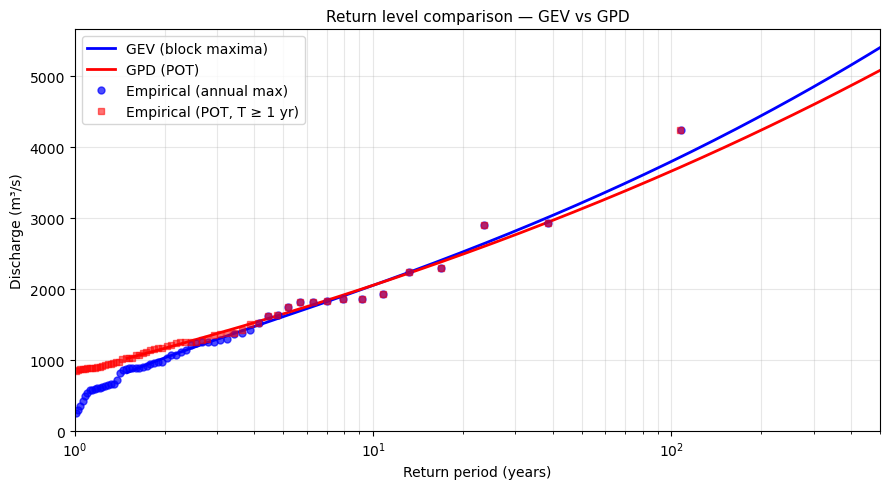
\includegraphics[width=0.88\linewidth]{figures/fig_gev_comparacion_notebook.png}
  \caption{Comparación de niveles de retorno obtenida en el notebook \texttt{climate/extreme\_value\_analysis.ipynb}. La curva azul corresponde al ajuste GEV sobre máximos anuales; la roja, al ajuste GPD sobre excedencias POT. Los puntos muestran posiciones empíricas de máximos anuales y excedencias POT con período de retorno anual o superior. Salida computada del notebook de análisis de extremos de \pyhydra.}
  \label{fig:gev_comparacion}
\end{figure}

Esta comparación no selecciona automáticamente un modelo; sirve como diagnóstico de coherencia entre enfoques de bloques máximos y umbrales. La elección final depende del tamaño muestral, la independencia de las excedencias, la estabilidad del umbral y el comportamiento de cola. Esta distinción es relevante para el diseño de \hydra: el módulo ofrece varios estimadores para facilitar el diagnóstico y la comparación, no para seleccionar uno de ellos sin evaluar los datos y los supuestos del caso.

La función \texttt{return\_levels} calcula los cuantiles para una lista de períodos de retorno a partir de los parámetros ajustados, con intervalos de confianza calculados por bootstrap o por la distribución posterior según el método empleado.

El diseño del módulo evita presentar un único estimador como solución universal. MLE es útil para diagnóstico rápido y muestras largas; L-momentos suele ser más estable en muestras cortas; MCMC permite comunicar incertidumbre paramétrica de forma explícita, pero exige revisar convergencia y sensibilidad a priors. La comparación entre métodos, más que la elección automática de uno, es el valor operativo de \pyhydra en episodios extremos como Valencia 2024.

\section{Análisis espacial}

\subsection{Análisis de frecuencia regional}

El módulo \texttt{spatial\_analysis.rfa} implementa el análisis de frecuencia regional (AFR) mediante el método del índice de avenida (\emph{index-flood}) \parencite{hosking1997rfa} basado en L-momentos. El procedimiento sigue las etapas estándar:
\begin{enumerate}
  \item Ajuste de GEV en cada estación, por máxima verosimilitud (\texttt{fit\_gev\_mle}), L-momentos (\texttt{fit\_gev\_lmom}, requiere \texttt{lmoments3}) o inferencia bayesiana (\texttt{fit\_gev\_bayes}).
  \item Diagnóstico regional mediante el estadístico de discordancia de Hosking--Wallis (\texttt{regional\_discordancy}) y el estadístico de heterogeneidad $H_1$ (\texttt{regional\_heterogeneity}), cuando el número y longitud de las estaciones permiten interpretarlos.
  \item Normalización de cada serie por su índice de avenida —la media de sus máximos anuales— mediante \texttt{regional\_index\_flood}.
  \item Ajuste de la distribución regional sobre los datos normalizados agrupados (\texttt{fit\_regional\_gev}).
  \item Reconversión a cuantiles locales por estación mediante el índice de avenida (\texttt{regional\_return\_levels}).
\end{enumerate}

La función \texttt{fit\_regional\_gev} acepta un diccionario de series de estación y devuelve los parámetros regionales junto con la serie de índices de avenida; \texttt{regional\_return\_levels} aplica el reescalado a cada estación para una lista de períodos de retorno. Además de los ajustes MLE y por L-momentos, la API admite \texttt{method=\textquotesingle{}bayes\textquotesingle{}}, que devuelve medianas e intervalos creíbles de cuantiles regionales escalados por estación. Los diagnósticos de discordancia y heterogeneidad ayudan a detectar estaciones incompatibles o regiones no homogéneas, pero no sustituyen el criterio hidrológico: la delimitación regional debe justificarse por coherencia climática, topográfica y pluviométrica antes de interpretar el ajuste. Su aplicación al caso Valencia 2024 \parencite{navas2025valenciaIA} con tres escalas espaciales (individual, regional local con 9 estaciones, regional global para toda la Comunidad Valenciana) ilustra cómo la elección de la escala de pooling modifica sustancialmente los períodos de retorno estimados del evento.

La implementación conserva explícitamente la relación entre estación, región homogénea y factor local de escala. Esta información es necesaria para auditar si una estación se está beneficiando legítimamente de información regional o si se está mezclando con estaciones de régimen pluviométrico distinto. En regiones mediterráneas o de fuerte gradiente orográfico, esta comprobación es tan importante como el ajuste de la distribución final.

\subsection{Cópulas}

El módulo \texttt{spatial\_analysis.copulas} implementa la clase \texttt{FloodEventCopula} para modelización multivariante de eventos de crecida \parencite{genest2007copulas,salvadori2007extremes}. La arquitectura separa el ajuste de marginales del ajuste de la estructura de dependencia:
\begin{enumerate}
  \item Las marginales se ajustan de forma independiente para cada variable (pico, duración, volumen) mediante GEV o GPD.
  \item La estructura de dependencia se representa mediante una cópula gaussiana ajustada sobre los rangos de los datos transformados a escala uniforme.
  \item El método \texttt{.sample(n)} genera $n$ realizaciones sintéticas del vector multivariante respetando las marginales y la dependencia observada.
\end{enumerate}

Este generador de eventos multivariantes es el núcleo del flujo estocástico para inundaciones \parencite{navas2018besaya,navas2019mallorca,navas2024calle30}. Su ventaja respecto a generadores univariantes es que conserva la estructura de dependencia entre pico, duración y volumen del hidrograma, lo que es determinante para la evaluación de obras de regulación y sistemas complejos.

La arquitectura de \texttt{FloodEventCopula} está concebida para admitir distintas familias de cópulas como estructura de dependencia. Las vine cópulas \parencite{aas2009vines} extienden el modelo gaussiano descomponiendo la densidad multivariante en un producto de cópulas bivariantes condicionadas que siguen una estructura jerárquica de árboles (R-vine o C-vine). Esta descomposición permite incluir familias asimétricas como la Gumbel o Joe, capaces de representar dependencias de cola superior que las cópulas elípticas no pueden capturar. La aplicación al río Besaya con cinco estaciones y 70 años de registros diarios \parencite{urrea2026vine} confirma esta superioridad de forma cuantitativa: la vine flexible obtiene un AIC mediano de $-5{,}04$ frente a $3{,}91$ de la vine gaussiana y $3{,}94$ de la cópula gaussiana con agrupación, con un RMSE de reproducción de la dependencia de cola superior de 0,11 frente a 0,30 de los enfoques gaussianos. El nivel crítico de Kendall para el JRP de 100 años es $t = 0{,}993$ para vine flexible frente a $t = 0{,}778$ para la cópula gaussiana sin agrupación, diferencia que se traduce en una tormenta de diseño multivariante un 36\% más intensa (63,45~mm frente a 46,49~mm de precipitación media areal). Para hacer viable el cálculo de la JCDF en cinco dimensiones, ese trabajo introduce además un emulador GPR con núcleo Racional Cuadrático que reduce el coste computacional en un 94\% respecto al cálculo directo por Monte Carlo, con MAE de $9{,}25 \times 10^{-4}$ y una incertidumbre propagada a las tormentas de diseño de $\pm 1{,}44$~mm. Estos avances representan la línea de extensión natural del módulo \texttt{spatial\_analysis.copulas} de \hydra para análisis multivariante en alta dimensión. Debe quedar claro el estado de implementación: la versión actual de \pyhydra incluye la cópula gaussiana multivariante de \texttt{FloodEventCopula} y las familias bivariantes de \texttt{BivariateCopula}; las vine cópulas y el emulador GPR proceden de un trabajo del grupo validado externamente \parencite{urrea2026vine} y no forman todavía parte del paquete.

\paragraph{Análisis de eventos compuestos bivariantes.}
El módulo implementa además la clase \texttt{BivariateCopula} para el análisis de eventos compuestos formados por dos variables de naturaleza distinta ---por ejemplo, caudal máximo y nivel del mar, precipitación y oleaje, o caudal y precipitación en cuencas con régimen mixto---. A diferencia de \texttt{FloodEventCopula}, que caracteriza un evento de crecida en sus dimensiones de pico, duración y volumen, \texttt{BivariateCopula} está diseñada para cuantificar la dependencia entre dos \emph{drivers} de peligrosidad independientes que pueden concurrir y amplificar mutuamente el impacto, el caso típico de la inundación costera compuesta \parencite{zscheischler2020compound}.

La clase admite tres familias paramétricas: \emph{Gumbel} (dependencia de cola superior, apropiada cuando los extremos conjuntos son más frecuentes de lo que implicaría la independencia), \emph{Clayton} (dependencia de cola inferior) y \emph{Frank} (simétrica). El ajuste comprende la estimación de las marginales paramétricas de cada variable y la estimación del parámetro de la cópula por máxima verosimilitud. El grado de dependencia se cuantifica mediante la $\tau$ de Kendall, que es función del parámetro de cópula y permite comparar familias entre sí.

El producto principal del análisis es el diagrama de períodos de retorno conjuntos, que distingue dos definiciones complementarias:
\begin{description}
  \item[$T_{\mathrm{OR}}$] Período de retorno de un evento que supera los umbrales de $X$ \emph{o} $Y$. Define la región de excedencia más amplia y es el criterio relevante cuando el impacto se produce si \emph{cualquiera} de las dos variables es extrema.
  \item[$T_{\mathrm{AND}}$] Período de retorno de un evento que supera los umbrales de $X$ \emph{y} $Y$ simultáneamente. Produce isolíneas más conservadoras y corresponde al criterio de diseño cuando ambos \emph{drivers} deben actuar de forma conjunta para generar un impacto.
\end{description}

Sobre cada isolínea de período de retorno se calcula el \emph{Evento de Diseño de Máxima Probabilidad} (\textsc{mpde}, \emph{Maximum Probability Design Event}): el punto de la isolínea con mayor densidad de probabilidad conjunta, estimado como el máximo del producto de la densidad de la cópula por las densidades marginales \parencite{salvadori2007extremes}. El \textsc{mpde} es el escenario de diseño más probable entre todos los que comparten un mismo período de retorno conjunto y constituye el candidato natural cuando se necesita un único vector de variables de entrada para el modelo hidráulico. La herramienta web de \hydra expone este análisis de forma interactiva mediante la aplicación \emph{Eventos Compuestos} disponible en el módulo \texttt{/tools/compound}.

\begin{figure}[htbp]
  \centering
  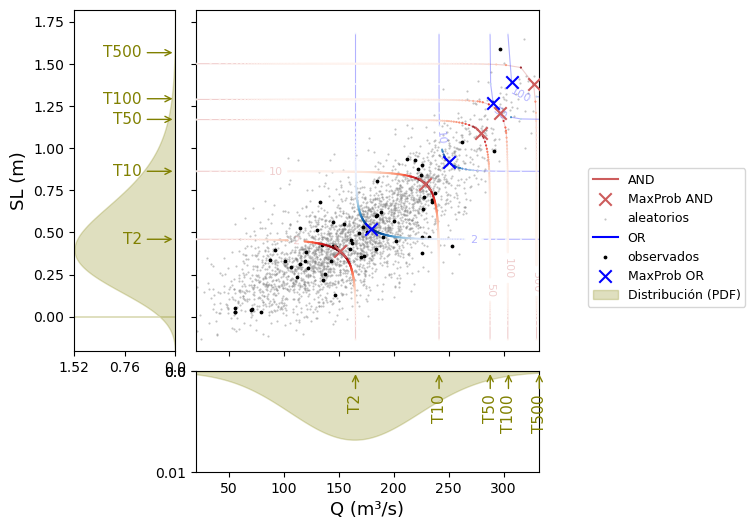
\includegraphics[width=\linewidth]{figures/fig_copula_joint_ret}
  \caption{Diagrama de períodos de retorno conjuntos AND y OR para un dataset sintético de caudal máximo ($Q_{\max}$, m$^3$/s) y nivel del mar (m) con cópula de Gumbel ajustada ($\tau_K \approx 0{,}52$). Las isolíneas AND (rojo) representan la condición de excedencia simultánea de ambas variables; las isolíneas OR (azul) la excedencia de al menos una de ellas. Los marcadores $\times$ señalan el \textsc{mpde} para cada período de retorno. Las distribuciones marginales ajustadas se muestran en los ejes superior y derecho. Elaboración propia a partir del notebook \texttt{compound\_flooding.ipynb}.}
  \label{fig:copula_joint_ret}
\end{figure}

\begin{figure}[htbp]
  \centering
  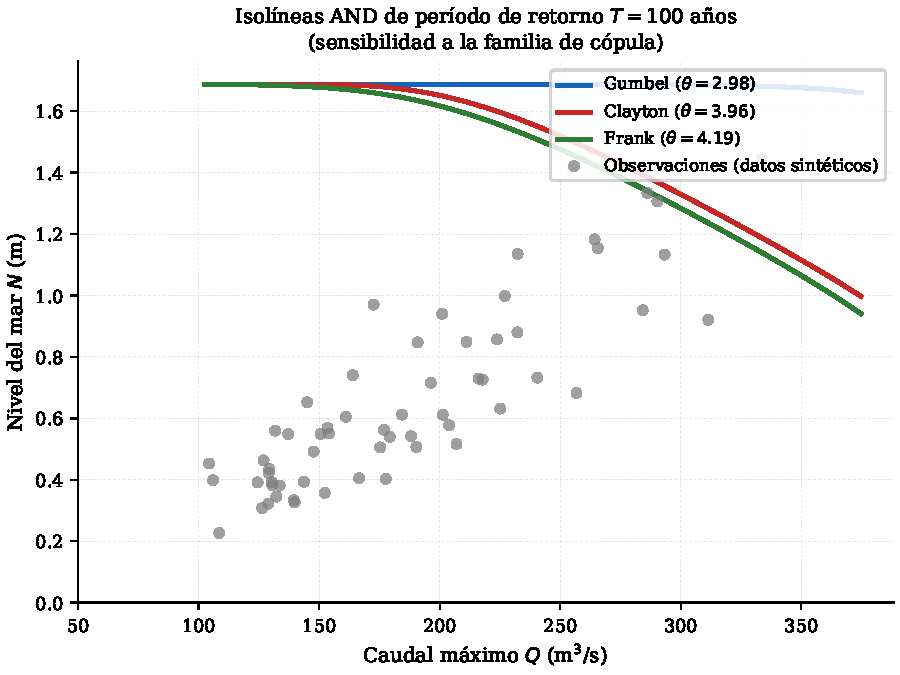
\includegraphics[width=\linewidth]{figures/fig_copula_familias}
  \caption{Comparación de las isolíneas AND de período de retorno $T=100$ años para tres familias de cópulas (Gumbel, Clayton y Frank) ajustadas sobre el mismo dataset. La familia Gumbel concentra la probabilidad conjunta en la cola superior (dependencia extrema simultánea), Clayton en la cola inferior y Frank produce isolíneas simétricas. La elección de familia modifica significativamente la región de diseño para el mismo período de retorno. Elaboración propia a partir del notebook \texttt{compound\_flooding.ipynb}.}
  \label{fig:copula_familias}
\end{figure}

\subsection{Interpolación geoestadística}

El módulo de interpolación espacial, \path{spatial_analysis.interpolation}, proporciona las clases \texttt{IDWInterpolator} y \texttt{KrigingInterpolator} para interpolar campos de estaciones a malla regular, además de \texttt{GaussianProcessInterpolator} para regresión por proceso gaussiano con covariables. Soporta así dos familias de métodos: inverso de la distancia ponderado (IDW) y kriging ordinario o universal con deriva externa (elevación, coordenadas u otra covariable). El kriging universal con elevación como variable auxiliar fue el método utilizado en el caso de Mallorca \parencite{navas2019mallorca} para la asignación de precipitación a subcuencas desde los pluviómetros disponibles.

La interpolación se trata como un módulo de análisis espacial, no como un mero preprocesado gráfico. La elección entre IDW, kriging ordinario y kriging universal depende de la densidad de estaciones, la relación con covariables topográficas y la escala del fenómeno. Cuando se usa elevación o precipitación media satelital como deriva externa, el módulo conserva esa covariable junto al campo interpolado para que el resultado pueda reproducirse.

\subsection{Modelos jerárquicos bayesianos}

El módulo \path{spatial_analysis.bayes_hierarchical} implementa la clase \texttt{HierarchicalGEV} para análisis regional con estructura jerárquica. El modelo asume que los parámetros de la distribución de extremos en cada localización son realizaciones de una distribución común de nivel superior (hiperpriors poblacionales), lo que permite transferir información entre estaciones y estimar cuantiles en puntos con muestras cortas. La inferencia se realiza mediante MCMC completo, con PyMC como motor por defecto y PyStan \parencite{carpenter2017stan} como alternativa. La clase expone \texttt{.fit(data\_dict)} para calibrar el modelo, \texttt{.posterior\_summary()} para resumir la posterior de los parámetros poblacionales y por estación, y \texttt{.return\_levels(credible=0.95)} para los cuantiles de período de retorno con su intervalo de credibilidad. A diferencia de enfoques basados en aproximaciones de Laplace anidadas (INLA) \parencite{rue2009inla}, la implementación actual no aproxima la posterior: la calcula por muestreo completo, lo que es más costoso computacionalmente pero evita las hipótesis de regularidad que exige INLA.

\section{Generación estocástica}

\subsection{Precipitación estocástica: NEOPRENE y CoSMoS}

El submódulo \texttt{stochastic\_generation} integra NEOPRENE como librería backend para generación estocástica de precipitación \parencite{diezsierra2023neoprene}. La clase \texttt{NSRPModel} envuelve la implementación puntual del proceso de Neyman-Scott de pulsos rectangulares \parencite{rodriguezituribe1987,rodriguezituribe1988}. El proceso NSRP es un modelo de eventos clusterizados donde cada tormenta madre genera un número aleatorio de células de lluvia con inicio, intensidad y duración extraídas de distribuciones paramétricas. La calibración ajusta los parámetros del proceso para reproducir estadísticos observados de la serie horaria o diaria: media, varianza, probabilidad de precipitación nula, correlación lag-1 y coeficiente de variación. La clase \texttt{STNSRPModel} envuelve la implementación multisitio de NEOPRENE, que extiende NSRP a estaciones correlacionadas y permite la generación de campos de precipitación espacialmente coherentes.

La diferencia entre \texttt{NSRPModel} y \texttt{STNSRPModel} es operativa. El primero es adecuado cuando se necesita una serie sintética representativa de un punto o estación; el segundo se utiliza cuando la coherencia espacial entre estaciones es parte del problema, por ejemplo para alimentar subcuencas simultáneamente o reconstruir campos multisitio. En ambos casos, \pyhydra actúa como envoltorio de NEOPRENE y estandariza entradas, salidas y configuración, pero no modifica la formulación estadística del modelo.

La serie temporal de caudal se puede también generar estocásticamente mediante el conjunto de funciones que el submódulo \texttt{stochastic\_generation.point} expone como envoltorio de la librería externa CoSMoS (\emph{Complete Stochastic Modelling Solution}) \parencite{papalexiou2018storm}: \texttt{fit\_distribution} y \texttt{fit\_acs} calibran, respectivamente, la marginal y la estructura de autocorrelación estacional; \texttt{analyze\_ts} encadena ambos ajustes sobre una serie diaria; y \texttt{simulate\_ts}/\texttt{generate\_ts} producen las realizaciones sintéticas. Este enfoque genera series preservando simultáneamente la distribución marginal, la dependencia temporal y la estacionalidad de la variable simulada. En \pyhydra se utiliza como generador general de series hidrológicas cuando el objetivo es producir realizaciones temporales largas de caudal o precipitación a partir de una estructura estadística calibrada, en contraste con NEOPRENE, que contiene NSRP y STNSRP y representa explícitamente la estructura física de la precipitación mediante tormentas y células.

La elección entre NEOPRENE y CoSMoS depende del objeto del estudio. NEOPRENE es preferible cuando interesa representar precipitación como proceso de tormentas y células, especialmente en aplicaciones espaciales de lluvia. CoSMoS es más general cuando la variable puede tratarse como serie temporal con una marginal y una estructura de dependencia temporal objetivo, por ejemplo caudal o variables hidroclimáticas agregadas. Mantener ambos enfoques permite cubrir problemas de inundación por eventos y problemas de recurso hídrico o clima de largo plazo.

\subsection{Campos espaciales}

El módulo \texttt{stochastic\_generation.fields} genera campos de precipitación en malla a partir de campos analíticos parametrizados o por interpolación de realizaciones puntuales del STNSRP. Sus salidas son \texttt{DataArray} con dimensiones \texttt{(realización, tiempo, lat, lon)}, compatibles directamente con los módulos de downscaling híbrido y de modelización hidrológica.

Estos campos no sustituyen a un modelo atmosférico regional; son escenarios estadísticos espacialmente coherentes para alimentar modelos hidrológicos o explorar sensibilidad. Por ello, el módulo registra la semilla, la malla, los parámetros de variograma o interpolación y las estaciones de origen. Sin esos metadatos, un campo sintético sería difícilmente auditable.

\section{Corrección de sesgo}

El submódulo \texttt{climate.bias\_correction} proporciona cuatro variantes para corregir las diferencias sistemáticas entre modelos climáticos y observaciones de referencia \parencite{teutschbein2012biascorrection}, accesibles mediante la función \texttt{delta\_method} y la clase \texttt{BiasCorrection}:

\begin{description}
  \item[\texttt{delta\_method}] Corrección aditiva (para temperatura) o multiplicativa (para precipitación) que aplica el cambio relativo del modelo climático mes a mes entre el período histórico de control y el período futuro, preservando el valor medio observado. Es el método más conservador y el preferido cuando se quiere minimizar la interferencia sobre la señal de cambio climático.

  \item[\texttt{BiasCorrection.quantile\_mapping}] Mapeo cuantil empírico aditivo (EQM): mapea la distribución empírica del modelo en el período histórico sobre la distribución observada y aplica la corrección resultante al período de proyección.

  \item[\texttt{BiasCorrection.quantile\_deltamapping}] Variante multiplicativa del mapeo cuantil empírico (QDM), más adecuada para precipitación.

  \item[\texttt{BiasCorrection.scaled\_distribution\_mapping}] SDM paramétrico \parencite{switanek2017sdm}: ajusta distribuciones gamma (precipitación) o normal (temperatura) a las tres series y preserva explícitamente los cambios de frecuencia e intensidad proyectados por el modelo climático. Es la variante recomendada cuando la magnitud del cambio en extremos es relevante.
\end{description}

El método \texttt{BiasCorrection.fit\_transform(obs, hist, future, var, method=\text{\textquotesingle}delta\text{\textquotesingle})} ofrece un punto de entrada único a las cuatro variantes sin necesidad de instanciar la clase explícitamente.

Ambos métodos fueron aplicados en los estudios de los países andinos \parencite{paz2019idb,deljesus2020andinos} y en SIMPCCe \parencite{navas2025simpce}, con proyecciones CMIP5 y CMIP6 respectivamente.

En \pyhydra, la corrección de sesgo se implementa como transformación explícita entre una serie o campo del modelo climático y una referencia observacional. El módulo conserva el período de calibración, la fuente observada, el modelo, el escenario y la variante de corrección. Esta trazabilidad es crítica porque dos estudios con el mismo modelo CMIP6 pueden producir resultados distintos si cambian el período histórico, la fuente observacional o la variante de mapeo cuantil.

\section{Downscaling híbrido}

El submódulo \texttt{climate.hybrid\_downscaling} implementa la cadena metodológica que conecta eventos sintéticos o escenarios seleccionados con mapas de inundación a escala de cuadrícula \parencite{navas2019mallorca,navas2024calle30}. La cadena consta de cuatro pasos:

\begin{enumerate}
  \item \textbf{Selección de eventos representativos (MaxDiss).} La función \path{maxdiss}, situada en \path{hybrid_downscaling.reconstruction}, selecciona un subconjunto de $n$ escenarios representativos del espacio total de eventos mediante el algoritmo de máxima disimilitud \parencite{camus2011maxdiss}. El algoritmo construye iterativamente un conjunto que maximiza la distancia mínima entre cualquier par de escenarios, cubriendo el espacio de variabilidad con el mínimo número de simulaciones. El submódulo \path{hybrid_downscaling.classification} complementa esta selección con \texttt{HydrographClassifier}, que agrupa formas de hidrograma por PCA y \emph{k}-means para organizar espacialmente los tipos representativos.

  \item \textbf{Simulación hidráulica del subconjunto.} Los $n$ eventos seleccionados se simulan con el modelo hidráulico (HEC-RAS, SFINCS) para obtener mapas de calado y velocidad.

  \item \textbf{Reconstrucción por vecinos próximos (k-NN).}\par
  La clase \path{FloodMapInterpolator} forma parte del submódulo de interpolación del downscaling híbrido. Entrena un modelo k-NN sobre los descriptores de evento y los mapas simulados. Una vez entrenado, reconstruye el mapa de inundación de cualquier evento del conjunto completo a partir de la interpolación ponderada de sus $k$ vecinos más próximos en el espacio de descriptores. En el caso de Calle 30 \parencite{navas2024calle30}, este enfoque permitió reconstruir miles de escenarios de inundación a partir de un conjunto de simulaciones explícitas mucho menor.

  \item \textbf{Mapas de período de retorno.} La función \texttt{pixel\_return\_period} en \texttt{hybrid\_downscaling.return\_period} calcula, para cada pixel de la malla, la distribución de calado máximo sobre el conjunto de escenarios y sus tasas de ocurrencia anuales, produciendo un mapa de nivel de retorno para cada período de retorno solicitado. La función \texttt{save\_return\_period\_geotiffs} exporta estos mapas en formato GeoTIFF georreferenciado.
\end{enumerate}

La \cref{fig:maxdiss_downscaling} resume la lógica operativa del método. El bloque superior representa la cadena estadística: datos históricos, extracción y descripción de eventos, generación sintética de $N$ realizaciones y selección MaxDiss del subconjunto representativo $n$. El bloque inferior representa la cadena física: preparación del dominio hidráulico, simulación explícita de los $n$ eventos seleccionados, construcción de una biblioteca de mapas de calado y reconstrucción k-NN de los mapas del conjunto completo. Las salidas de auditoría intermedias (tabla de eventos, listado de casos a simular, GeoTIFF intermedios) garantizan la trazabilidad de cada resultado.

\begin{figure}[!htbp]
\centering
\resizebox{\textwidth}{!}{%
\begin{tikzpicture}[
  font=\scriptsize,
  node distance=0.78cm and 0.78cm,
  arr/.style={-Stealth, line width=0.8pt, color=tg55},
  data/.style={rectangle, rounded corners=3pt, draw=blue!55!black, fill=blue!8,
	               text width=2.48cm, minimum height=0.78cm, align=center},
  stat/.style={rectangle, rounded corners=3pt, draw=orange!70!black, fill=orange!12,
	               text width=2.48cm, minimum height=0.78cm, align=center},
  model/.style={rectangle, rounded corners=3pt, draw=teal!65!black, fill=teal!10,
	                text width=2.48cm, minimum height=0.78cm, align=center},
  outputbox/.style={rectangle, rounded corners=3pt, draw=red!55!black, fill=red!8,
	              text width=2.48cm, minimum height=0.78cm, align=center},
  group/.style={rectangle, rounded corners=5pt, draw=tg40, dashed, inner sep=0.18cm},
  dot/.style={circle, fill=#1, minimum size=0.16cm, inner sep=0}
]

% Main methodological chain
\node[data] (obs) {Datos históricos\\caudal o lluvia};
\node[stat, right=of obs] (events) {Extracción y\\descripción de eventos};
\node[stat, right=of events] (synthetic) {Generación sintética\\$N$ eventos};
\node[stat, right=of synthetic] (maxdiss) {MaxDiss\\$n \ll N$ eventos};

\node[model, below=1.05cm of maxdiss] (hydraulic) {Simulación hidráulica\\eventos $n$};
\node[model, left=of hydraulic] (maps) {Biblioteca\\calado/velocidad};
\node[model, left=of maps] (knn) {Reconstrucción k-NN\\resto de eventos};
\node[outputbox, left=of knn] (risk) {Mapas finales\\período de retorno};

\draw[arr] (obs) -- (events);
\draw[arr] (events) -- (synthetic);
\draw[arr] (synthetic) -- (maxdiss);
\draw[arr] (maxdiss.south) -- (hydraulic.north);
\draw[arr] (hydraulic) -- (maps);
\draw[arr] (maps) -- (knn);
\draw[arr] (knn) -- (risk);

% Inputs from hydraulic domain
\node[data, below=0.85cm of hydraulic] (terrain) {MDE, rugosidad,\\malla y contornos};
\draw[arr] (terrain.north) -- (hydraulic.south);

% Audit products
\node[outputbox, above=0.75cm of events] (audit1) {Tabla de eventos\\y descriptores};
\node[outputbox, above=0.75cm of maxdiss] (audit2) {Listado de casos\\a simular};
\node[outputbox, below=0.75cm of maps] (audit3) {GeoTIFF/NetCDF\\intermedios};
\draw[arr] (events.north) -- (audit1.south);
\draw[arr] (maxdiss.north) -- (audit2.south);
\draw[arr] (maps.south) -- (audit3.north);

\end{tikzpicture}
}
\caption{Esquema operativo del downscaling híbrido implementado en \hydra. La metodología separa la generación estadística masiva de eventos ($N$ escenarios) de la simulación hidráulica completa: MaxDiss selecciona un subconjunto representativo $n \ll N$ que cubre el espacio de variabilidad, ese subconjunto se simula con el modelo físico, y los mapas del conjunto restante se reconstruyen por k-NN. Las salidas de auditoría intermedias permiten trazar cada resultado hasta su configuración de datos y simulación. Elaboración propia.}
\label{fig:maxdiss_downscaling}
\end{figure}

Este flujo, denominado \emph{downscaling híbrido} porque combina selección estadística con reconstrucción por aprendizaje automático, reduce el coste computacional de la metodología estocástica en varios órdenes de magnitud respecto a simular todos los eventos \parencite{deljesus2024downscaling}. Su validez exige descriptores hidráulicamente informativos y un subconjunto MaxDiss representativo del espacio de variabilidad.

\subsection{Validación de la reconstrucción k-NN}
\label{sec:validacion_knn}

La reconstrucción k-NN es la pieza que hace viable la metodología estocástica, y por tanto su error debe cuantificarse en cada aplicación en lugar de asumirse. El protocolo de validación integrado en el flujo es la validación cruzada sobre el propio subconjunto simulado: se excluye una simulación (o un pliegue de ellas), se reconstruye su mapa a partir de las restantes mediante \texttt{FloodMapInterpolator} y se compara la reconstrucción con la simulación física excluida. Sobre cada par reconstruido--simulado se calculan tres familias de métricas complementarias: error de calado por píxel (RMSE y sesgo medio, restringidos a la zona inundada); acierto en extensión sobre un umbral de calado, resumido mediante el índice de acierto crítico (CSI) y las tasas de sobrepredicción e infrapredicción; y error en los cuantiles altos de la distribución de calados, que son los que gobiernan los mapas de período de retorno.

Este análisis cumple tres funciones operativas. Primero, dimensionar el subconjunto MaxDiss: si el error de validación cruzada no se estabiliza al aumentar $n$, el subconjunto no cubre suficientemente el espacio de variabilidad. Segundo, diagnosticar los descriptores: errores concentrados en un tipo de evento indican que el espacio de características no captura alguna dimensión hidráulicamente relevante (forma del hidrograma, simultaneidad entre subcuencas). Tercero, acotar la incertidumbre de reconstrucción que se propaga a los mapas de período de retorno, de modo que pueda declararse junto al resto de fuentes de incertidumbre del estudio. En las aplicaciones de la línea (Mallorca, Calle 30, Panamá) la verificación se realizó mediante la comparación de mapas reconstruidos frente a simulados durante el desarrollo de cada estudio; la sistematización de estas métricas como salida estándar del módulo, con informe automático de validación cruzada por caso, forma parte de los criterios de aceptación recogidos en el \cref{ch:casos_estudio}.

\chapter{Modelización hidrológica e hidráulica}
\label{ch:modelización}

\section{Rol de \hydra en la cadena metodológica}
\label{sec:rol_hydra}

\hydra no sustituye las metodologías hidrológicas, hidráulicas, climáticas o estadísticas existentes. Actúa como marco de integración capaz de coordinar estas metodologías dentro de una cadena de cálculo reproducible. Los motores de simulación conservan exactamente su comportamiento; los métodos estadísticos se invocan con las mismas formulaciones que en la literatura de referencia; los datos se obtienen de las mismas fuentes institucionales. La aportación de \hydra es la capa de orquestación que conecta cada uno de estos componentes, estandariza sus interfaces y los hace operables de forma conjunta.

La \cref{tab:componentes_hydra} resume los componentes de la cadena y las herramientas o metodologías que \hydra incorpora en cada bloque.

Este capítulo se centra en la parte física de la cadena: la transformación de escenarios climáticos, hidrológicos o sintéticos en respuestas de caudal, calado, velocidad y extensión inundada. En una metodología estocástica, esta transformación no puede hacerse manualmente caso a caso. Cada escenario debe generar entradas de modelo, ejecutarse con una configuración controlada y producir salidas comparables. El bloque de modelización existe precisamente para convertir modelos profesionales ya aceptados en piezas de una cadena repetible.

\begin{table}[htbp]
  \centering
  \caption{Componentes de la cadena metodológica de \hydra y herramientas o metodologías incorporadas.}
  \label{tab:componentes_hydra}
  \begin{tabular}{p{0.30\textwidth}p{0.60\textwidth}}
    \toprule
    Componente & Herramienta o metodología \\
    \midrule
    Fuentes de datos & ERA5, GPM/IMERG, PERSIANN, AEMET, OGIMET, Meteostat, GloFAS, GRDC, USGS, SoilGrids \\[3pt]
    Análisis de extremos & GEV/GPD · L-momentos · Inferencia bayesiana (PyMC, PyStan opcional) \\[3pt]
    Análisis multivariante & Cópulas gaussianas · Vine cópulas \\[3pt]
    Generación estocástica & NEOPRENE (NSRP puntual y STNSRP multisitio) · CoSMoS \\[3pt]
    Cambio climático & CMIP6 (CDS/ESGF) bajo escenarios SSP \\[3pt]
    Corrección de sesgo & Delta method · Quantile mapping \\[3pt]
    Downscaling híbrido & MaxDiss · k-NN \\[3pt]
    Emulación & Gaussian Process Regression (GPR) \\[3pt]
    Modelización hidrológica & HEC-HMS · SWAT \\[3pt]
    Modelización hidráulica & SFINCS · HEC-RAS · Iber \\[3pt]
    \bottomrule
  \end{tabular}
\end{table}

En ningún caso \hydra propone estas metodologías como contribuciones nuevas: las implementa, las conecta y las hace operables de forma conjunta. Su contribución reside en que esa integración, antes inexistente o dependiente de flujos manuales frágiles, es ahora reproducible, auditable y transferible a nuevos casos sin reconstruir la cadena desde cero.

\section{Objetivo del bloque}

El bloque de modelización conecta los datos y escenarios generados por \hydra con modelos físicos ampliamente utilizados en ingeniería hidrológica e hidráulica. Su objetivo es reducir la carga manual asociada a la configuración, ejecución por lotes y postprocesado de resultados, sin reemplazar los motores físicos ni modificar su comportamiento.

La arquitectura del bloque sigue el patrón de adaptador. Cada módulo traduce estructuras de datos internas de \hydra al formato esperado por el modelo externo, lanza la ejecución y transforma las salidas a productos comunes: hidrogramas como \texttt{pandas.Series}, mapas de calado como \texttt{xarray.DataArray}, y tablas de resultados como \texttt{pandas.DataFrame}. Esta estrategia mantiene la independencia entre \hydra y los motores físicos: cuando aparece una nueva versión del modelo o un nuevo motor alternativo, solo es necesario actualizar el adaptador correspondiente.

El patrón de adaptador tiene cuatro responsabilidades concretas. Primero, preparar entradas: escribir ficheros de precipitación, caudal, condiciones de contorno o parámetros en el formato nativo de cada motor. Segundo, ejecutar: lanzar el motor mediante API, controlador externo o subproceso, registrando versión, ruta de ejecutable y código de salida. Tercero, leer resultados: convertir DSS, HDF, NetCDF, GeoTIFF o ficheros de texto en estructuras comunes. Cuarto, validar: comprobar que la simulación terminó, que existen salidas esperadas y que los valores tienen unidades y rangos plausibles. Esta separación evita que el análisis estadístico dependa de formatos propietarios.

La integración tiene también límites explícitos. HYDRA no calibra automáticamente cualquier modelo por el hecho de ejecutarlo; solo automatiza las operaciones implementadas y documentadas en cada adaptador. Tampoco sustituye la revisión hidráulica experta: la estabilidad numérica, la calidad del MDT, la rugosidad, las condiciones de contorno y la representación de estructuras siguen siendo decisiones técnicas del modelo físico.

\section{Modelos hidrológicos}

\subsection{HEC-HMS}

HEC-HMS \parencite{scharffenberg2016hechms} es el modelo de simulación hidrológica del Cuerpo de Ingenieros del Ejército de los Estados Unidos. Simula procesos de precipitación-escorrentía a escala de cuenca, integrando métodos de pérdidas, transformación precipitación-caudal y propagación en cauces. Su uso está muy extendido en administraciones hidráulicas españolas, lo que lo convierte en el motor hidrológico preferente para estudios integrados con planes de zona inundable.

En la cadena de \pyhydra, HEC-HMS ocupa el papel de traductor entre lluvia y caudal. Es especialmente útil en casos como Calle 30, donde el forzamiento estocástico se genera como precipitación multisitio y debe convertirse en hidrogramas de entrada para el modelo hidráulico. Esta separación permite mantener el análisis estadístico de lluvia en el bloque climático y la respuesta de cuenca en un motor hidrológico reconocido.

El módulo \texttt{modeling.hydrology.hec\_hms} encapsula el acceso a HEC-HMS a través de tres funcionalidades:

\begin{description}
  \item[Preparación de entradas.] Las funciones \texttt{generate\_gage} y \texttt{fill\_gage\_series} escriben las series de precipitación o caudal en formato DSS mediante \texttt{hecdss} (independiente de la versión de \texttt{numpy}, a diferencia de \texttt{pydsstools}); \texttt{generate\_met} y \texttt{generate\_hms} actualizan respectivamente el modelo meteorológico y la estructura principal del proyecto para enlazar pluviómetros, cuenca, control y ejecución.

  \item[Ejecución.] La función \texttt{run\_hms\_script} lanza HEC-HMS en modo batch mediante un script generado automáticamente (API Jython en Windows, \texttt{xvfb-run} en Linux) y espera a su finalización; \texttt{read\_hms\_dss\_timeseries} lee después las series de salida del DSS resultante. La clase \texttt{HMSModel} envuelve este ciclo completo: su método \texttt{.run\_hms(*params)} ejecuta el modelo con un vector de parámetros y devuelve el caudal simulado como \texttt{ndarray}, delegando en \texttt{run\_hms\_script} y en la lectura DSS. Este patrón admite la ejecución de múltiples simulaciones en bucle, lo que permite la simulación sistemática del conjunto de eventos estocásticos.

  \item[Calibración automática con spotpy.] \texttt{HMSModel} por sí sola no calibra: expone la interfaz de ejecución (\texttt{.run\_hms(*params)}, punto de extensión \texttt{.\_write\_params(params)}) que hace de ella una \emph{setup class} compatible con \texttt{spotpy} \parencite{houska2015spotpy}. Su subclase \texttt{TextBasinHMSCalibrationModel} implementa esa escritura de parámetros editando directamente el fichero \texttt{.basin} como factores multiplicativos sobre valores base. La función \texttt{calibrate\_hms\_sceua} invoca internamente el algoritmo SCE-UA (\emph{shuffled complex evolution}) de \texttt{spotpy} sobre un \texttt{TextBasinHMSCalibrationModel}, con la función objetivo (NSE, PBIAS o RMSE) configurable. La integración actual cubre SCE-UA; otros algoritmos de \texttt{spotpy} (PSO, DREAM, etc.) son utilizables sobre la misma \emph{setup class} pero no están envueltos en una función dedicada de \pyhydra.
\end{description}

La calibración automática fue especialmente relevante en el estudio de los países andinos \parencite{paz2019idb,deljesus2020andinos}, donde la escala territorial y el número de cuencas hizo inviable la calibración manual de los modelos hidrológicos. La integración de esa experiencia en \hydra generaliza la capacidad a cualquier proyecto que use HEC-HMS como motor hidrológico.

\subsection{SWAT}

SWAT \parencite{arnold1998swat,gassman2007swat} es un modelo hidrológico semidistribuido de simulación continua, desarrollado por el USDA-ARS. A diferencia de HEC-HMS, que opera a escala de evento, SWAT simula el ciclo hidrológico completo con paso diario durante períodos de años o décadas, lo que lo hace adecuado para evaluación de recursos hídricos, análisis de tendencias y escenarios de cambio climático a largo plazo.

Por esa razón, SWAT se conecta principalmente con el bloque de cambio climático. Las series históricas y futuras corregidas por sesgo se transforman en entradas meteorológicas continuas, se ejecutan por escenario y se comparan salidas agregadas como aportaciones mensuales, caudal medio o indicadores de sequía. El interés industrial no está solo en ejecutar SWAT, sino en repetir el mismo flujo sobre decenas de combinaciones modelo--escenario--horizonte sin perder trazabilidad.

El módulo \texttt{modeling.hydrology.swat} gestiona la integración mediante un conjunto de funciones, no una clase orientada a objetos:

\begin{description}
  \item[Preparación de entradas climáticas.] Las funciones \texttt{write\_precipitation\_file} y \texttt{write\_temperature\_file} convierten series de precipitación y temperatura (históricas o proyecciones CMIP6 corregidas) al formato clásico de ficheros \texttt{.pcp}/\texttt{.tmp} de SWAT a partir de coordenadas de estación y series diarias; \texttt{write\_swatplus\_precipitation\_files} y \texttt{write\_swatplus\_temperature\_files} generan el equivalente para SWAT+ (ficheros individuales por estación más el índice \texttt{pcp.cli}/\texttt{tmp.cli}); \texttt{edit\_file\_cio} ajusta el período de simulación en \texttt{file.cio}.

  \item[Ejecución por escenarios.] La función \texttt{run\_swat} lanza el ejecutable de SWAT+ en el directorio \texttt{TxtInOut} del proyecto y devuelve el código de salida del proceso.
\end{description}

La lectura de las salidas de SWAT (\texttt{output.rch}, \texttt{output.sub}) no está actualmente automatizada dentro de \pyhydra: se realiza de forma ad-hoc en cada caso de estudio, fuera del paquete. Completar un lector genérico de estos ficheros es trabajo pendiente (\cref{ch:conclusiones}).

SIMPCCe \parencite{navas2025simpce} es el ejemplo más directo de uso de SWAT dentro del ecosistema \hydra para análisis de aportaciones a embalses españoles bajo proyecciones CMIP6.

\section{Modelos hidráulicos}

\subsection{SFINCS}

SFINCS \parencite{leijnse2021sfincs} (Super-Fast INundation of CoastS) es un modelo hidráulico bidimensional de física reducida desarrollado por Deltares. Su formulación simplificada de las ecuaciones de Saint-Venant reduce drasticamente el tiempo de computo manteniendo una precisión aceptable para inundación urbana y costera, lo que lo convierte en el motor preferente para flujos estocásticos con alto número de escenarios.

La ventaja de SFINCS dentro de \hydra es su escalabilidad. Al usar mallas regulares o cuasi-regulares y ficheros de configuración simples, se presta bien a la generación automática de proyectos y a la ejecución masiva. Esto lo convierte en una opción adecuada para atlas nacionales, análisis de sensibilidad o cribados iniciales donde el número de escenarios pesa más que el detalle hidráulico local.

El módulo \texttt{modeling.hydraulic.sfincs} proporciona:
\begin{description}
  \item[\texttt{setup\_sfincs\_model}] Configura la malla de cálculo a partir de geometría de cuenca, modelo digital de elevaciones, puntos de entrada y series de caudal. Devuelve un objeto \texttt{SfincsModel} que se persiste en disco mediante \texttt{mod.write()}.

  \item[\texttt{run\_sfincs}] Ejecuta SFINCS para el proyecto configurado en un directorio de trabajo.

  \item[\texttt{write\_manning\_wl\_boundary}] Escribe una condición de contorno de nivel aguas abajo calculada mediante Manning y actualiza los ficheros \texttt{sfincs.bnd}, \texttt{sfincs.bzs} y \texttt{sfincs.inp}.
\end{description}

La lectura de resultados SFINCS se concentra actualmente en \path{modeling.hydraulic.sensitivity}, mediante \path{load_sfincs_ensemble}. Esta función lee la variable \path{hmax} de los ficheros \path{sfincs_map.nc} producidos por ejecuciones en lote, georreferencia las coordenadas del modelo y devuelve un \path{xarray.DataArray} con una dimensión de simulación. Esta separación refleja el uso operativo del módulo: \path{sfincs.py} prepara y ejecuta proyectos, mientras que \path{sensitivity.py} agrega y analiza ensembles de resultados.

\subsection{HEC-RAS}

HEC-RAS \parencite{brunner2016hecras} es la referencia profesional más extendida para modelización hidráulica 1D/2D en administraciones y consultoría española. La memoria del MITECO para cartografía de zonas inundables \parencite{marm2011guia} referencia HEC-RAS como herramienta principal, lo que hace que una fracción significativa de los modelos hidráulicos calibrados en España estén en este formato.

En \hydra, HEC-RAS cubre dos necesidades distintas. En modelos 1D, como Calle 30, permite representar redes de conducción, tramos canalizados o sistemas lineales donde la geometría hidráulica está definida por secciones y conectividad. En modelos 2D, como los análisis posteriores del Besaya, permite obtener campos espaciales de calado y velocidad comparables con SFINCS. El adaptador actual se centra en preparar escenarios, modificar ficheros de proyecto y lanzar ejecuciones; la extracción espacial de resultados 2D se realiza en los flujos de postproceso de los casos, pero no está expuesta como función pública independiente en \texttt{pyhydra.modeling.hydraulic.hec\_ras}.

El módulo \texttt{modeling.hydraulic.hec\_ras} automatiza cuatro operaciones:
\begin{description}
  \item[\texttt{modify\_unsteady\_file}] Actualiza el fichero de flujo no permanente de HEC-RAS con una nueva serie de caudal, permitiendo simular diferentes escenarios sin modificar manualmente el proyecto.

  \item[\texttt{modify\_plan\_file} y \texttt{modify\_project\_file}] Actualizan el plan y el proyecto para activar el nuevo fichero de flujo no permanente.

  \item[\texttt{create\_flow\_series}] Suaviza series de caudal mediante máximo móvil centrado antes de escribirlas como condición de contorno.

  \item[\texttt{run\_hec\_ras}] Lanza el plan activo de HEC-RAS mediante \texttt{rascontrol}, condicionado a disponer de una instalación local compatible.
\end{description}

Su uso en Calle 30 \parencite{navas2024calle30} y en desarrollos posteriores sobre el entorno del Besaya demuestra la viabilidad de la automatización incluso en proyectos de complejidad industrial. La limitación principal es que HEC-RAS no dispone de una API pública documentada y estable para todos los modos de control externo, por lo que la integración se basa en la modificación de ficheros de texto, la ejecución del ejecutable vía subproceso o controlador disponible y la lectura sistemática de salidas.

\subsection{Iber}

Iber \parencite{blade2014iber} es un modelo hidráulico bidimensional de superficie libre desarrollado por el CEDEX y la Universidad de A Coruña. Su integración en el flujo de trabajo de \hydra se limita en la versión actual a la preparación de entradas (hidrogramas de entrada en el formato de ficheros de texto de Iber) y a la lectura de resultados exportados a GeoTIFF desde la interfaz gráfica. No se ha implementado un adaptador de automatización completo porque Iber no dispone de una API de línea de comandos documentada que permita la ejecución en modo \textit{batch} sin interacción con la interfaz gráfica, lo que hace inviable su uso en flujos estocásticos con cientos o miles de simulaciones. Esta limitación es la razón técnica por la que HEC-RAS y SFINCS, que sí admiten ejecución automatizada mediante subproceso o controlador externo, sustituyeron progresivamente a Iber en los desarrollos posteriores. La integración parcial es coherente con su papel en los trabajos iniciales de la línea, especialmente el Besaya \parencite{navas2018besaya} y Mallorca \parencite{navas2019mallorca}, donde se empleó para las simulaciones individuales del subconjunto representativo antes de que los adaptadores de HEC-RAS y SFINCS estuvieran disponibles.

\section{Análisis de sensibilidad}
\label{sec:sensibilidad}

El módulo \texttt{modeling.hydraulic.sensitivity} proporciona herramientas para análisis de sensibilidad de parámetros hidráulicos (rugosidad de Manning, condiciones de contorno) mediante ejecuciones sistemáticas del modelo con variaciones paramétricas. Su desarrollo recoge funciones generales surgidas durante el análisis del río Besaya \parencite{navas2025roughness}, pero los notebooks empleados para preparar ese artículo constituyen material interno de investigación y no forman parte de los ejemplos de uso de \hydra.

El objetivo del módulo no es sustituir un estudio de incertidumbre completo, sino facilitar el muestreo y la comparación sistemática de respuestas hidráulicas. En el caso del Besaya, el parámetro analizado fue la rugosidad de Manning por clases de uso del suelo; en otros dominios podrían analizarse condiciones de contorno, niveles aguas abajo o parámetros de infiltración. La estructura común es siempre la misma: generar un ensemble de configuraciones, ejecutar el modelo, cargar resultados y resumir la variabilidad de las métricas de impacto.

Las \cref{fig:manning_distributions,fig:sensibilidad_manning} ilustran los resultados obtenidos en el análisis de sensibilidad de Manning sobre el caso del río Besaya. La \cref{fig:manning_distributions} contrasta los valores bibliográficos, las distribuciones ajustadas y las muestras Monte Carlo para nueve clases de uso del suelo. La \cref{fig:sensibilidad_manning} resume primero el ensemble de entradas y después la respuesta intramodelo de SFINCS y HEC-RAS.

\begin{figure}[htbp]
  \centering
  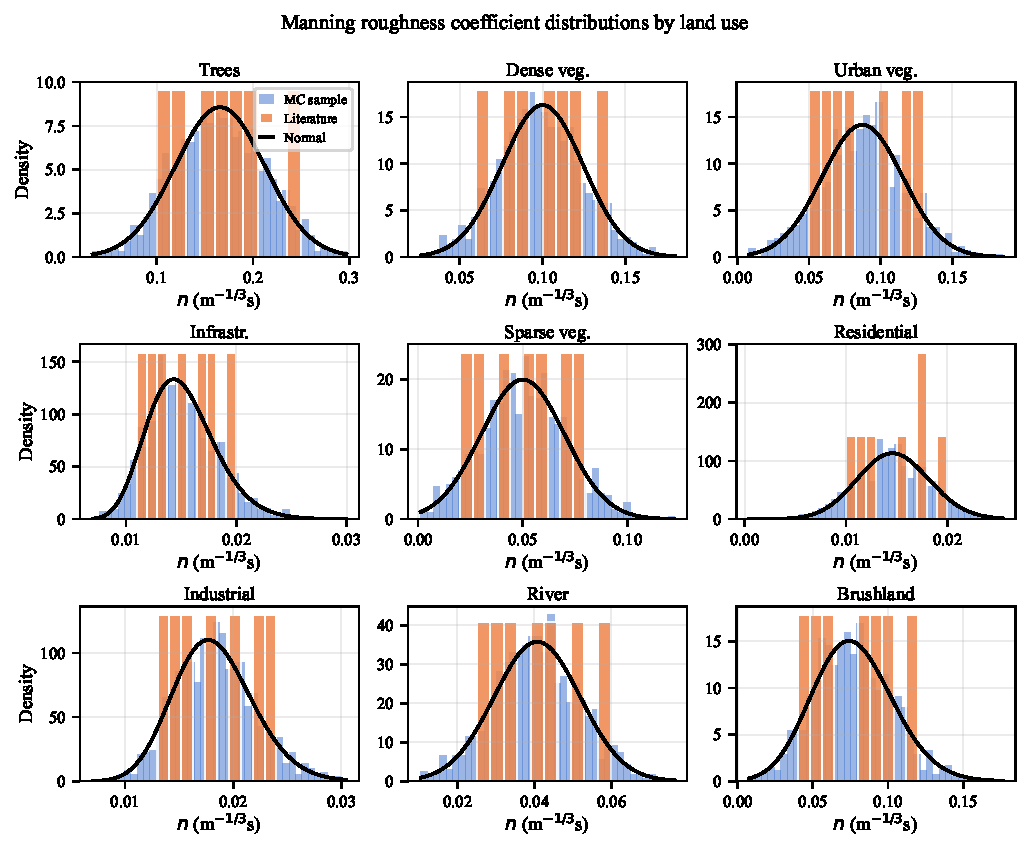
\includegraphics[width=0.75\textwidth]{figures/besaya_fig01_manning_distributions.pdf}
  \caption{Distribuciones ajustadas del coeficiente de Manning para nueve clases de uso del suelo en Los Corrales de Buelna. Los histogramas azules representan las 1.000 muestras Monte Carlo; las barras naranjas, los valores bibliográficos de referencia; y las curvas negras, la distribución seleccionada mediante el contraste de Kolmogorov--Smirnov. Fuente: \parencite{navas2025roughness}.}
  \label{fig:manning_distributions}
\end{figure}

\begin{figure}[htbp]
  \centering
  \begin{subfigure}[b]{0.48\textwidth}
    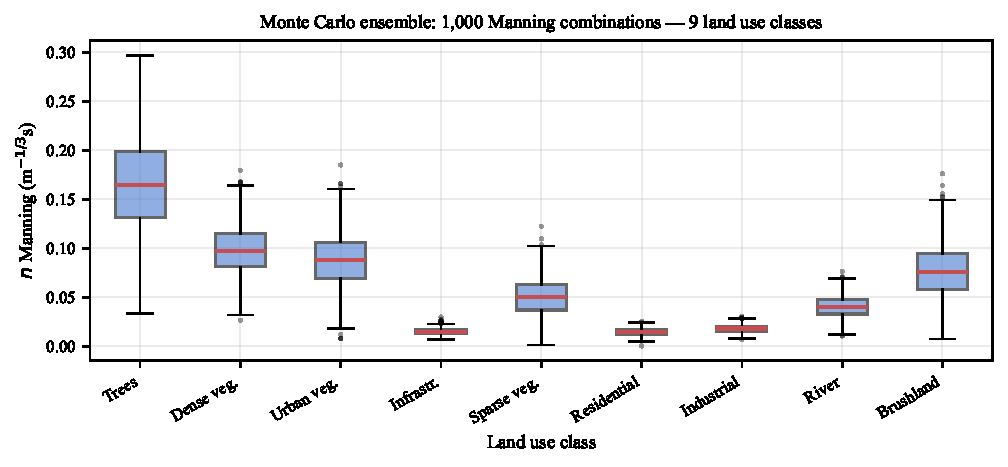
\includegraphics[width=\textwidth]{figures/besaya_fig02_mc_boxplots.pdf}
    \caption{Distribución de Manning del ensemble por clase de uso.}
    \label{fig:mc_boxplots}
  \end{subfigure}
  \hfill
  \begin{subfigure}[b]{0.48\textwidth}
    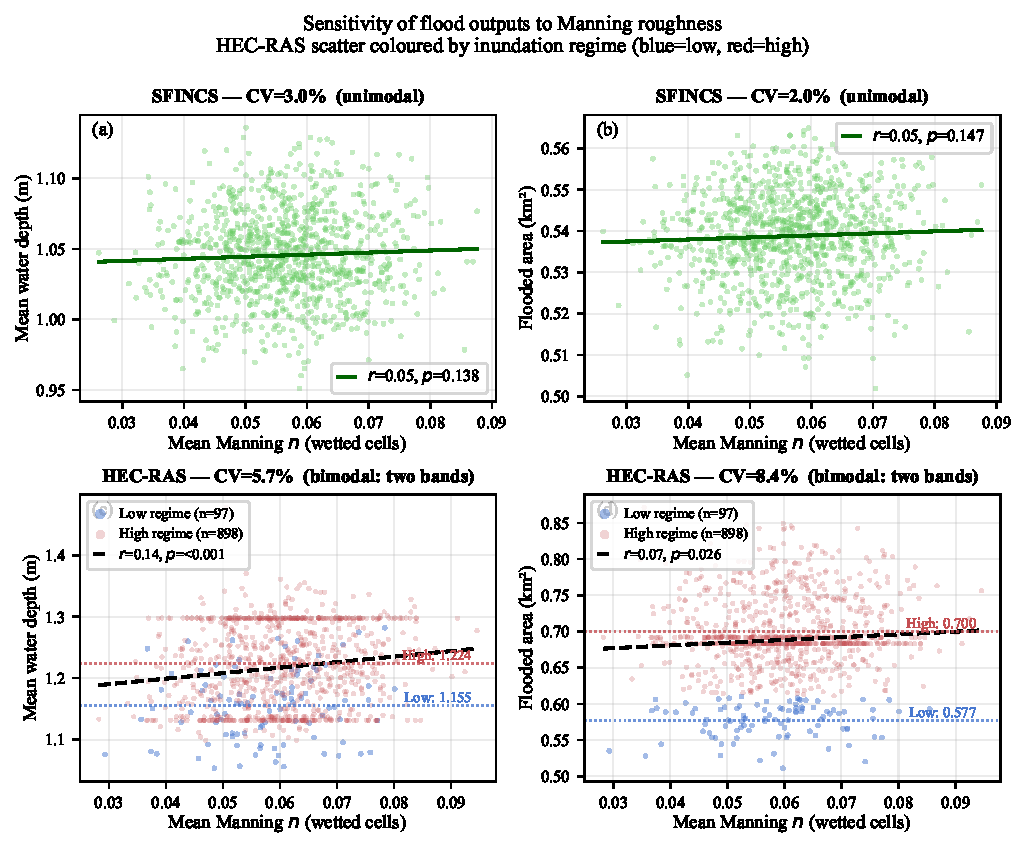
\includegraphics[width=\textwidth]{figures/besaya_fig03_intramodel_sensitivity.pdf}
    \caption{Manning medio frente a calado y área inundada.}
    \label{fig:intramodel}
  \end{subfigure}
  \caption{Ensemble y respuesta hidráulica del análisis de sensibilidad en Los Corrales de Buelna. Izquierda: boxplots de las 1.000 combinaciones de Manning para las nueve clases de uso. Derecha: relación entre Manning medio, calado medio y área inundada para SFINCS y HEC-RAS; las dos bandas de HEC-RAS corresponden a dos regímenes de inundación identificados mediante un modelo de mezcla gaussiana. Fuente: \parencite{navas2025roughness}.}
  \label{fig:sensibilidad_manning}
\end{figure}

\section{Postprocesado y métricas de impacto}

Una vez ejecutados los modelos hidrológicos e hidráulicos, \hydra transforma sus resultados en métricas de impacto comparables entre escenarios. Esta fase es conceptualmente la más importante del flujo: el objetivo final no es producir hidrogramas o mapas de calado, sino cuantificar la probabilidad de superar umbrales de impacto relevantes.

Las métricas disponibles incluyen:
\begin{itemize}
  \item calado máximo por pixel para cada evento o escenario;
  \item velocidad máxima y producto calado-velocidad como indicador de peligrosidad;
  \item extensión inundada sobre un umbral de calado definido por el usuario;
  \item período de retorno por pixel calculado sobre el conjunto de escenarios mediante \texttt{pixel\_return\_period};
  \item hidrograma de caudal punta y volumen de evento en puntos de control.
\end{itemize}

La combinación de estas métricas con los mapas de exposición y vulnerabilidad del territorio permite construir indicadores de riesgo específicos del caso de estudio, cerrando el flujo desde datos climáticos hasta información útil para la toma de decisiones.

El postprocesado mantiene separadas tres capas: salida física del modelo, métrica de impacto y producto de decisión. Un GeoTIFF de calado máximo es una salida física; el período de retorno por pixel es una métrica probabilística; y un mapa clasificado por umbrales de afección es un producto de decisión. Separar estas capas evita confundir el resultado numérico del modelo con la interpretación de riesgo que se realiza posteriormente.

\chapter{Manual práctico de HYDRA}
\label{ch:manual}

\section{Instalación}

El objetivo de este capítulo es proporcionar una ruta práctica para ejecutar los flujos principales con el menor número posible de decisiones ambiguas. El usuario puede trabajar de dos formas complementarias: instalando \pyhydra como librería Python, recomendado para desarrollo y uso desde scripts propios; o mediante la plataforma \hydra con Docker, recomendada para reproducir los notebooks, navegar la web y ejecutar los servicios sin configurar manualmente el entorno.

\begin{table}[htbp]
  \centering
  \caption{Formas recomendadas de uso de \pyhydra y \hydra.}
  \label{tab:manual_modos_uso}
  \begin{tabular}{p{0.28\textwidth}p{0.28\textwidth}p{0.32\textwidth}}
    \toprule
    Modo & Uso recomendado & Ventaja principal \\
    \midrule
    Instalación editable de \pyhydra & Desarrollo de módulos y uso desde scripts propios & Iteración rápida sobre el código fuente del núcleo \\
    \hydra + Docker + JupyterLab & Reproducir notebooks, revisar ejemplos completos y usar la web & Entorno cerrado con dependencias controladas \\
    \bottomrule
  \end{tabular}
\end{table}

Para instalación directa del núcleo \pyhydra en el entorno Python del usuario:

\begin{codeblock}
git clone https://github.com/navass11/pyhydra.git
cd pyhydra
pip install -e .
\end{codeblock}

La versión instalada puede comprobarse desde Python:

\begin{codeblock}
import pyhydra
print(pyhydra.__version__)
\end{codeblock}

\subsection{Despliegue del entorno Docker}

El entorno Docker pertenece al repositorio \hydra y es la vía recomendada cuando se quieren ejecutar los notebooks de ejemplo sin gestionar manualmente las dependencias. La imagen JupyterLab incluye \pyhydra con todas las dependencias extendidas ya instaladas (PyMC, NEOPRENE, HydroMT, hecdss, GeoPandas, etc.) y arranca JupyterLab en el puerto 8888. Para iniciar el entorno completo:

\begin{codeblock}
git clone https://github.com/navass11/HYDRA.git
cd HYDRA
docker compose -f docker/docker-compose.yml up -d
\end{codeblock}

Por defecto los datos se montan desde el subdirectorio \texttt{data/} del repositorio. Para apuntar a un directorio distinto (por ejemplo, un recurso compartido con proyectos de modelización ya existentes):

\begin{codeblock}
HYDRA_DATA_PATH="/ruta/a/datos" \
  docker compose -f docker/docker-compose.yml up -d
\end{codeblock}

El servicio \texttt{web} expone una interfaz de navegación de notebooks en el puerto 80. El acceso a JupyterLab se realiza en \texttt{http://localhost/jupyter/} y el backend de herramientas en \texttt{http://localhost/api/}.

\begin{figure}[p]
  \centering
  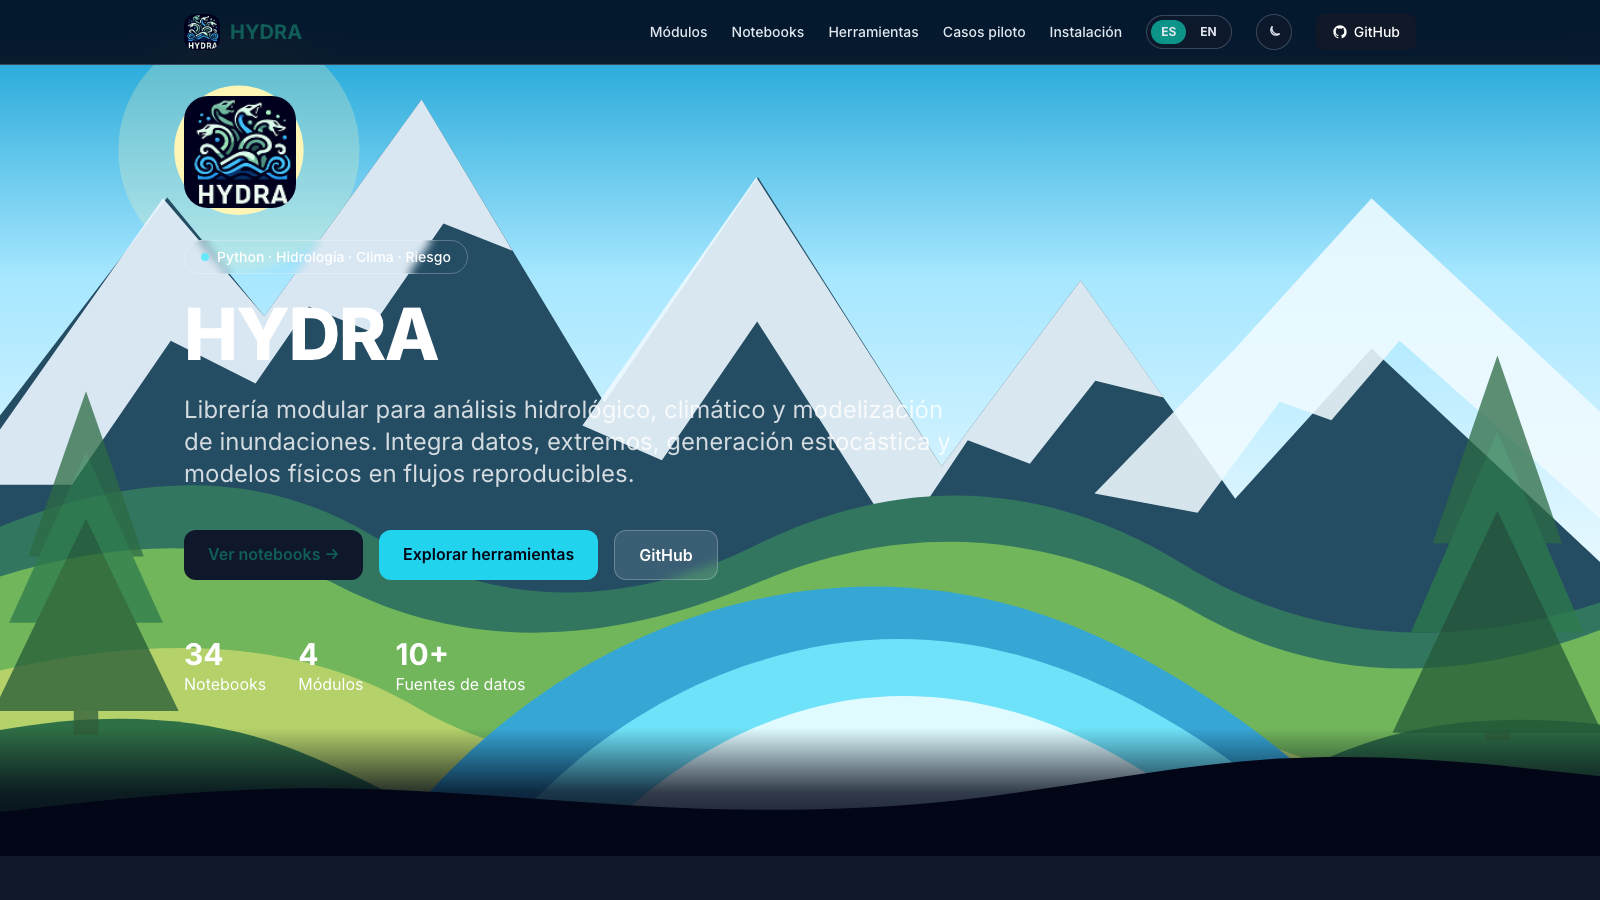
\includegraphics[width=0.96\textwidth]{figures/fig_hydra_web_home.png}
  \caption{Pantalla principal de la web de \hydra exportada desde el material de presentación de la tesis. La interfaz actúa como punto de entrada a los módulos, notebooks, herramientas, casos piloto e instalación, y traduce el núcleo \pyhydra a una experiencia navegable para usuarios técnicos.}
  \label{fig:hydra_web_home}
\end{figure}

\section{Criterios de uso como producto industrial}

\hydra se documenta en esta memoria como un \emph{framework} operativo ---no solo como un conjunto de scripts de investigación---. Por ello, cada flujo debe poder evaluarse con cuatro criterios: entrada trazable, transformación reproducible, salida estándar y registro suficiente para auditar el resultado. La \cref{tab:manual_contratos} resume estos contratos de uso.

\begin{table}[htbp]
  \centering
  \caption{Contratos operativos que debe cumplir un flujo reproducible con \hydra.}
  \label{tab:manual_contratos}
  \begin{tabular}{p{0.21\textwidth}p{0.25\textwidth}p{0.36\textwidth}}
    \toprule
    Elemento & Ejemplos & Requisito práctico \\
    \midrule
    Entradas & CSV, NetCDF, GeoTIFF, GeoJSON, DSS, ficheros HEC-RAS/HEC-HMS & Conservar fuente, fecha de descarga, versión del producto y sistema de referencia. \\
    Configuración & JSON/YAML, argumentos Python, parámetros de modelo & Separar parámetros del código y registrar umbrales, períodos, escenarios y semillas aleatorias. \\
    Salidas intermedias & Eventos, parámetros, hidrogramas, mapas simulados & Guardar productos que sean costosos de regenerar o necesarios para auditar decisiones. \\
    Salidas finales & Tablas, GeoTIFF, figuras, mapas de período de retorno & Exportar en formatos interoperables y acompañados de metadatos espaciales y temporales. \\
    \bottomrule
  \end{tabular}
\end{table}

La librería sigue una convención de datos sencilla: las series temporales se representan como \texttt{pandas.Series} o \texttt{pandas.DataFrame} con \texttt{DatetimeIndex}; los campos espaciales como \texttt{xarray.DataArray}, \texttt{xarray.Dataset} o raster GeoTIFF; y los modelos externos se tratan como proyectos versionables en disco. Esta decisión evita formatos propietarios dentro del núcleo de \pyhydra y facilita la integración con herramientas de consultoría, administración y visualización.

\section{Estructura del paquete}

\pyhydra se organiza en tres bloques principales que reflejan directamente la arquitectura descrita en el \cref{ch:arquitectura}:

\begin{itemize}
  \item \texttt{pyhydra.data\_sources} --- descarga, lectura y estandarización de fuentes de datos;
  \item \texttt{pyhydra.climate} --- análisis estadístico, generación estocástica, corrección de sesgo y downscaling;
  \item \texttt{pyhydra.modeling} --- automatización de modelos hidrológicos e hidráulicos.
\end{itemize}

Cada bloque expone sus funciones y clases principales directamente desde su \texttt{\_\_init\_\_.py}, de modo que el patrón de importación es siempre del tipo:

\begin{codeblock}
from pyhydra.climate.time_series import fit_gev, extract_block_maxima
from pyhydra.modeling.hydrology.hec_hms import HMSModel
from pyhydra.modeling.hydraulic.sfincs import setup_sfincs_model
\end{codeblock}

Los 26 notebooks generales de ejemplo catalogados por la web, excluyendo casos piloto y material interno de preparación de artículos, funcionan como guías ejecutables de las funcionalidades del paquete. La \cref{tab:notebooks} lista su correspondencia con los módulos. El catálogo fuente de la interfaz web contiene además 23 entradas de casos piloto, usadas para recorrer flujos completos de Besaya, M-30, Manning y Valencia desde el navegador.

\begin{figure}[htbp]
  \centering
  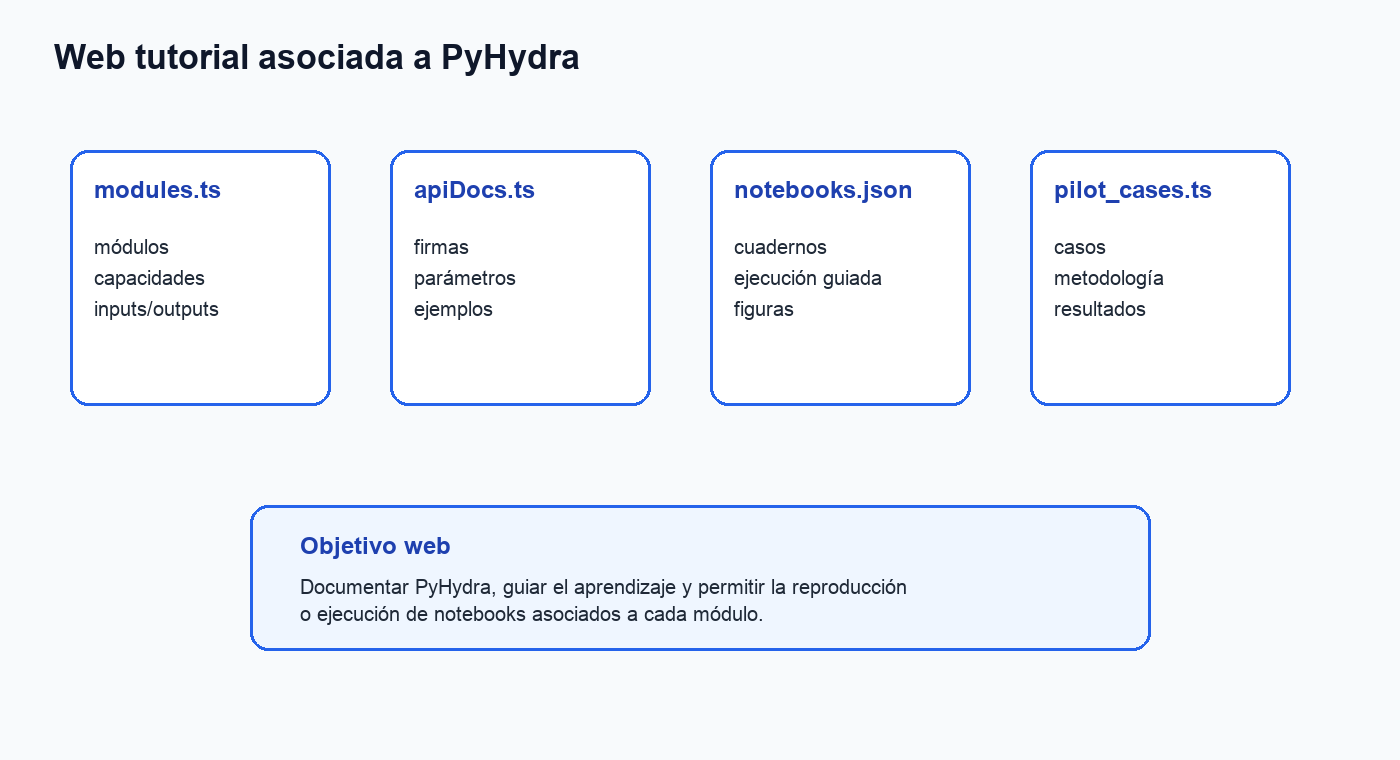
\includegraphics[width=0.94\textwidth]{figures/fig_hydra_web_tutorial.png}
  \caption{Estructura tutorial de la web asociada a \pyhydra. Los ficheros de catálogo conectan módulos, referencia de API, notebooks reproducibles y casos piloto, de modo que la documentación no queda separada del código ni de las evidencias computacionales usadas en la tesis.}
  \label{fig:hydra_web_tutorial}
\end{figure}

\begin{table}[htbp]
  \centering
  \caption{Responsabilidad técnica de cada bloque principal de \pyhydra.}
  \label{tab:manual_responsabilidades}
  \begin{tabular}{p{0.26\textwidth}p{0.31\textwidth}p{0.31\textwidth}}
    \toprule
    Bloque & Responsabilidad & Salida típica \\
    \midrule
    \texttt{data\_sources} & Obtener y normalizar datos externos sin alterar el dato bruto original. & NetCDF, CSV estandarizado, GeoTIFF, metadatos de descarga. \\
    \texttt{climate} & Transformar series y campos en eventos, distribuciones, escenarios sintéticos y productos estadísticos. & Tablas de eventos, parámetros, series sintéticas, mapas de retorno. \\
    \texttt{modeling} & Traducir datos internos de \hydra a los formatos de modelos físicos y recuperar resultados. & Proyectos HEC-HMS/HEC-RAS/SFINCS/SWAT, hidrogramas, rasters de calado. \\
    \bottomrule
  \end{tabular}
\end{table}

\small
\begin{longtable}{>{\raggedright\arraybackslash}p{0.55\textwidth}>{\raggedright\arraybackslash}p{0.33\textwidth}}
  \caption{Correspondencia entre notebooks y módulos de \pyhydra.}
  \label{tab:notebooks} \\
  \toprule
  Notebook & Módulo \pyhydra \\
  \midrule
  \endfirsthead
  \toprule
  Notebook & Módulo \pyhydra \\
  \midrule
  \endhead
  \path{data_sources/climate_change/CDS_download} & \path{data_sources.climate_change} \\
  \path{data_sources/climate_change/ESGF_download} & \path{data_sources.climate_change} \\
  \path{data_sources/rainfall/ERA5_download} & \path{data_sources.rainfall} \\
  \path{data_sources/rainfall/GPM_download} & \path{data_sources.rainfall} \\
  \path{data_sources/rainfall/PERSSIAN_download} & \path{data_sources.rainfall} \\
  \path{data_sources/rainfall/AEMET_download} & \path{data_sources.rainfall} \\
  \path{data_sources/rainfall/OGIMET_download} & \path{data_sources.rainfall} \\
  \path{data_sources/rainfall/Meteostat_download} & \path{data_sources.rainfall} \\
  \path{data_sources/river_discharge/GloFAS_download} & \path{data_sources.river_discharge} \\
  \path{data_sources/river_discharge/GRDC_download} & \path{data_sources.river_discharge} \\
  \path{data_sources/river_discharge/USGS_download} & \path{data_sources.river_discharge} \\
  \path{data_sources/soils/SoilGrids_download} & \path{data_sources.soils} \\
  \path{climate/event_extraction} & \path{climate.time_series} \\
  \path{climate/extreme_value_analysis} & \path{climate.time_series} \\
  \path{climate/spatial_analysis/regional_frequency_analysis} & \path{climate.spatial_analysis} \\
  \path{climate/spatial_analysis/bayes_hierarchical} & \path{climate.spatial_analysis} \\
  \path{climate/spatial_analysis/copulas} & \path{climate.spatial_analysis} \\
  \path{climate/spatial_analysis/compound_flooding} & \path{climate.spatial_analysis} \\
  \path{climate/spatial_analysis/interpolation} & \path{climate.spatial_analysis} \\
  \path{climate/stochastic_generation} & \path{climate.stochastic_generation} \\
  \path{climate/spatial_field_generation} & \path{climate.stochastic_generation} \\
  \path{climate/bias_correction} & \path{climate.bias_correction} \\
  \path{modeling/hydrology/HEC_HMS} & \path{modeling} \\
  \path{modeling/hydrology/SWAT} & \path{modeling} \\
  \path{modeling/hydraulic/SFINCS} & \path{modeling} \\
  \path{modeling/hydraulic/HEC_RAS} & \path{modeling} \\
  \bottomrule
\end{longtable}
\normalsize

\subsection{Notebooks como especificación ejecutable}

La documentación del producto no se apoya solo en la lectura del código fuente. Cada bloque de la librería se valida mediante notebooks que actúan como ejemplos reproducibles: contienen una descripción metodológica, datos sintéticos o de referencia, llamadas a la API y productos de salida. Esta estructura es especialmente importante en una tesis industrial, porque permite demostrar que \hydra no es un prototipo aislado, sino una herramienta con flujos de uso comprobables.

Además de los notebooks funcionales generales, el directorio del caso piloto de Los Corrales de Buelna, situado en \texttt{notebooks/pilot\_cases/}, documenta el origen de la línea metodológica. Este material complementa el capítulo de casos de estudio porque muestra el encadenamiento completo de la librería desde adquisición de datos hasta mapas de período de retorno.

\begin{table}[htbp]
  \centering
  \small
  \caption{Flujo del caso piloto de Los Corrales de Buelna documentado en notebooks.}
  \label{tab:manual_corrales_notebooks}
  \begin{tabular}{>{\raggedright\arraybackslash}p{0.34\textwidth}>{\raggedright\arraybackslash}p{0.25\textwidth}>{\raggedright\arraybackslash}p{0.29\textwidth}}
    \toprule
    Notebook & Módulos implicados & Función en el flujo \\
    \midrule
    \texttt{01\_data\_acquisition} & datos externos & Recopilación y organización inicial de series y cartografía. \\
    \texttt{02\_spatial\_interpolation} & \texttt{spatial\_analysis} & Reconstrucción espacial mediante IDW y kriging. \\
    \texttt{03\_extreme\_value\_analysis} & \path{time_series.extremes} & Ajuste GEV/GPD y curvas de período de retorno. \\
    \texttt{04\_design\_storm\_hms} & \texttt{modeling.hydrology} & Preparación de tormentas de diseño y entradas HEC-HMS. \\
    \texttt{05\_continuous\_simulation} & modelos externos & Simulación continua y gestión de hidrogramas. \\
    \shortstack[l]{\texttt{06\_hybrid\_event\_}\\\texttt{reconstruction}} & \texttt{hybrid\_downscaling} & Selección de eventos, MaxDiss y reconstrucción de hidrogramas. \\
    \texttt{07\_hec\_ras\_hydraulics} & \texttt{modeling.hydraulic} & Automatización de HEC-RAS para casos representativos. \\
    \texttt{08\_hybrid\_return\_periods} & \texttt{hybrid\_downscaling} & Reconstrucción de mapas y períodos de retorno por pixel. \\
    \bottomrule
  \end{tabular}
\end{table}

\subsection{Qué puede ejecutar un tercero}
\label{sec:reproducibilidad_tercero}

La reproducibilidad de \hydra se entiende en términos concretos: qué puede ejecutar un tercero mañana, con qué datos y en qué tiempo. La siguiente tabla clasifica los elementos reproducibles por tipo de dependencia y resultado esperado.

\begin{table}[htbp]
  \centering
  \small
  \caption{Elementos reproducibles de \hydra clasificados por disponibilidad, datos y tiempo estimado de ejecución.}
  \label{tab:reproducibilidad}
  \begin{tabular}{p{0.23\textwidth}p{0.09\textwidth}p{0.13\textwidth}p{0.13\textwidth}p{0.28\textwidth}}
    \toprule
    Elemento & Disp. & Datos & Tiempo & Resultado esperado \\
    \midrule
    Ajuste GEV sintético (MLE, L-mom., bayesiano) & Sí & Sintéticos & $<$5 min & Curvas de período de retorno con bandas de incertidumbre (fig.~5.1) \\[3pt]
    Análisis de inundación compuesta (cópulas) & Sí & Sintéticos & $<$5 min & Isolíneas AND/OR, MPDE (fig.~5.2) \\[3pt]
    Generación estocástica NEOPRENE (NSRP/STNSRP) & Sí & Sintéticos & $<$15 min & Series de lluvia sintéticas puntuales y multisitio \\[3pt]
    Corrección de sesgo delta/EQM & Sí & Sintéticos o ERA5, CMIP6 & $<$10 min & NetCDF corregido con señal de cambio preservada \\[3pt]
    Interpolación espacial y AFR & Sí & Sintéticos o AEMET & $<$10 min & GeoTIFF interpolado, cuantiles regionales \\[3pt]
    Descarga ERA5 (requiere cuenta CDS) & Sí & API abierta & Horas & NetCDF ERA5 horario/mensual \\[3pt]
    Descarga CMIP6 (requiere cuenta CDS) & Sí & API abierta & Horas & NetCDF de proyecciones por modelo y escenario \\[3pt]
    Simulación HEC-HMS (requiere HEC-HMS) & Sí & Modelos de referencia & 10--60 min & Hidrogramas DSS para 200 eventos sintéticos \\[3pt]
    Flujo hidráulico completo con SFINCS & Parcial & DEM + hidrogramas & Horas--días & Mapas de calado por evento, períodos de retorno por pixel \\[3pt]
    Caso piloto completo (Corrales de Buelna) & Parcial & Datos abiertos + modelo & Días & Distribución de calados, mapa de período de retorno \\
    \bottomrule
  \end{tabular}
\end{table}

Los elementos marcados como ``Parcial'' requieren adicionalmente un modelo calibrado o una licencia de software específica. Los primeros seis ítems pueden ejecutarse sin más requisito que tener instalado \pyhydra o el entorno Docker; son los más adecuados para una primera evaluación del marco.

\section{Referencia de la API}
\label{sec:manual_wiki_api}

La referencia completa de la API de \pyhydra ---incluyendo la firma de cada función, sus parámetros y el tipo de objeto devuelto--- se recoge en el \cref{app:api}. Las secciones siguientes ilustran el uso de cada bloque funcional mediante ejemplos representativos orientados a la aplicación práctica.

% ============================================================
\section{Bloque de datos (\texttt{pyhydra.data\_sources})}
% ============================================================

El bloque de datos agrupa cuatro módulos de acceso a fuentes externas con interfaces homogéneas: \texttt{rainfall} (ERA5, GPM, PERSIANN-CCS, AEMET, OGIMET), \texttt{river\_discharge} (GloFAS, GRDC, USGS), \texttt{climate\_change} (CMIP6 vía Copernicus CDS y ESGF) y \texttt{soils} (SoilGrids). Todos los módulos devuelven \texttt{pandas.DataFrame} o \texttt{xarray.Dataset} con metadatos de trazabilidad, y pueden ejecutarse desde los notebooks de ejemplo que documentan el proceso completo con datos reales para cada caso de estudio. La referencia de parámetros para cada función se recoge en el \cref{app:api}.

El criterio de diseño es minimizar la configuración manual: credenciales, dominios espaciales y períodos temporales se declaran explícitamente en el notebook de cada caso, de modo que la ejecución sea repetible sin intervención adicional. Cuando una fuente requiere registro (CDS, NASA Earthdata, ESGF, AEMET OpenData), los notebooks incluyen instrucciones paso a paso para obtener las credenciales necesarias.

El siguiente ejemplo ilustra la descarga de precipitación ERA5 y la lectura posterior del fichero resultante:

\begin{codeblock}
from pyhydra.data_sources.rainfall import download_era5
import xarray as xr

# Descarga precipitación horaria sobre la Península Ibérica (1979-2023)
download_era5(
    folder_out="data/era5/",
    api_key="UID:API_KEY",          # credenciales ~/.cdsapirc
    url="https://cds.climate.copernicus.eu/api",
    area=[44, -10, 35, 5],          # [N, W, S, E]
    variables_list=["total_precipitation"],
    years=range(1979, 2024),
)

# Lectura del NetCDF descargado como xarray.Dataset
ds = xr.open_mfdataset("data/era5/*.nc", combine="by_coords")
precip = ds["tp"] * 1000           # conversión m → mm
\end{codeblock}

Para descarga de caudales de una estación GRDC, el módulo devuelve directamente un \texttt{DataFrame} con índice de fechas:

\begin{codeblock}
from pyhydra.data_sources.river_discharge.grdc import read_grdc

# Lectura de fichero GRDC descargado del portal GRDC
Q = read_grdc("data/grdc/6335060_Q_Day.Cmd.txt")
# Q: pd.DataFrame con columnas ["date", "discharge"] (m3/s, NaN si falta/marcado)
\end{codeblock}

% ============================================================
\section{Bloque climático y estadístico}
% ============================================================

El bloque \path{pyhydra.climate} opera sobre las series y campos producidos por el bloque de datos. Se organiza en cinco submódulos con responsabilidades bien delimitadas:

\begin{description}
  \item[\texttt{time\_series}.] Detección de eventos (\texttt{extract\_events}) y análisis de extremos: ajuste GEV y GPD con cinco métodos de estimación (MLE, L-momentos, MAP, Fisher e MCMC), cálculo de niveles de retorno con incertidumbre y diagnóstico gráfico.

  \item[\texttt{spatial\_analysis}.] Interpolación espacial (kriging, IDW), análisis de frecuencia regional por el método de inundación índice, modelo GEV jerárquico bayesiano, cópulas gaussianas para eventos multivariantes (\texttt{FloodEventCopula}) y cópulas bivariantes con períodos de retorno conjuntos AND/OR y evento de diseño de máxima probabilidad para análisis de inundación compuesta (\texttt{BivariateCopula}).

  \item[\texttt{stochastic\_generation}.] Generación estocástica de precipitación con NEOPRENE, tanto puntual (\texttt{NSRPModel}) como multisitio (\texttt{STNSRPModel}), y generación de series hidro-climáticas generales con CoSMoS. Incluye además la generación de campos aleatorios espacialmente coherentes basados en variogramas.

  \item[\texttt{bias\_correction}.] Corrección de sesgo de proyecciones CMIP6: método delta (\texttt{delta\_method}) y mapeo cuantil (EQM, QDM, SDM) implementados en la clase \texttt{BiasCorrection}, con un único punto de entrada \texttt{BiasCorrection.fit\_transform} para las cuatro variantes.

  \item[\texttt{hybrid\_downscaling}.] Selección de eventos representativos por máxima disimilitud, reconstrucción de hidrogramas, interpolación de manchas de inundación y estimación del período de retorno por pixel. Las clases principales son \path{FloodEventSelector}, \path{HydrographReconstructor}, \path{FloodMapInterpolator} y \path{pixel_return_period}.
\end{description}

El flujo habitual combina los submódulos en secuencia: los extremos calibran los generadores estocásticos, la corrección de sesgo ajusta las proyecciones climáticas, y el downscaling híbrido convierte la serie sintética en mapas de impacto. Cada submódulo puede utilizarse de forma independiente cuando el caso de estudio no requiere la cadena completa. Los notebooks de ejemplo ilustran configuraciones representativas para cada bloque; la referencia de parámetros se recoge en el \cref{app:api}.

El siguiente ejemplo muestra el ajuste de una distribución GEV sobre máximos anuales, la estimación del nivel de retorno a T\,=\,100 años con intervalo de confianza bootstrap, y la representación gráfica del diagnóstico:

\begin{codeblock}
from pyhydra.climate.time_series import (
    extract_block_maxima, fit_gev, return_levels, return_level_ci,
    plot_return_levels,
)

# 1. Máximos anuales de precipitación diaria
ams = extract_block_maxima(precip_series, freq="YE")

# 2. Ajuste GEV por máxima verosimilitud
params = fit_gev(ams.values, method="mle")
# params: {"mu": ..., "sigma": ..., "xi": ...}

# 3. Niveles de retorno para T = [10, 25, 50, 100, 200, 500] años
rl = return_levels(params, T_values=[10, 25, 50, 100, 200, 500])

# 4. Intervalo de confianza al 90% por bootstrap (MLE + remuestreo)
point, lower, upper = return_level_ci(
    ams.values, T=100, method="mle",
    n_bootstrap=500, ci=0.90,
)

# 5. Figura de diagnóstico (QQ, PP y curva de retorno)
plot_return_levels(ams.values, params, T_range=(1.5, 500))
\end{codeblock}

Para la corrección de sesgo de proyecciones CMIP6 con el método delta sobre precipitación:

{\footnotesize
\begin{codeblock}
from pyhydra.climate.bias_correction import BiasCorrection

precip_corrected = BiasCorrection.fit_transform(
    obs=precip_obs_monthly,        # pd.Series observada (período histórico)
    hist=precip_cmip6_hist,        # pd.Series modelo histórico
    future=precip_cmip6_ssp585,    # pd.Series modelo futuro
    var="pr",                      # variable ("pr" o "tas")
    method="delta",                # "delta" | "eqm" | "qdm" | "sdm"
)
\end{codeblock}
}

% ============================================================
\section{Bloque de modelización (\texttt{pyhydra.modeling})}
% ============================================================

El bloque de modelización expone interfaces de automatización para cuatro motores de simulación externos organizados en dos familias:

\begin{description}
  \item[Hidrología.] \texttt{modeling.hydrology.hec\_hms} envuelve HEC-HMS con funciones de preparación de entradas meteorológicas, escritura en formato DSS, parametrización automática a partir de datos geoespaciales (curva número, tiempo de concentración, Muskingum) y lectura de resultados. \texttt{modeling.hydrology.swat} prepara ficheros de forzamiento para SWAT+ y lanza el ejecutable con control del período de simulación.

  \item[Hidráulica.] \texttt{modeling.hydraulic.sfincs} configura proyectos SFINCS desde geometría, DEM y series de caudal, calcula la condición de contorno aguas abajo con Manning y lanza el ejecutable. La lectura de resultados SFINCS en ensemble se realiza actualmente desde \texttt{modeling.hydraulic.sensitivity} mediante \texttt{load\_sfincs\_ensemble}, que extrae \texttt{hmax} de los ficheros \texttt{sfincs\_map.nc}. \texttt{modeling.hydraulic.hec\_ras} modifica ficheros de proyecto no estacionario e inserta hidrogramas de contorno sin salir de Python.
\end{description}

El patrón de uso es consistente en todos los módulos: preparar los datos en formatos internos de \pyhydra, llamar a las funciones de configuración, ejecutar el motor y leer los resultados mediante funciones de postprocesado. Los adaptadores aislan al usuario del formato propietario de cada motor, de modo que puede sustituirse un modelo hidráulico por otro sin modificar el código de análisis estadístico. Los notebooks de ejemplo documentan configuraciones completas para los casos del Besaya (HEC-HMS + SFINCS), Calle 30 (HEC-HMS + HEC-RAS) y SIMPCCe (SWAT); la referencia de parámetros se recoge en el \cref{app:api}.

El siguiente ejemplo ilustra la configuración y ejecución de SFINCS para un conjunto de hidrogramas representativos:

{\footnotesize
\begin{codeblock}
from pyhydra.modeling.hydraulic.sfincs import setup_sfincs_model, run_sfincs
from pyhydra.modeling.hydraulic.sensitivity import load_sfincs_ensemble

# 1. Crear proyecto SFINCS a partir de DEM e hidrograma de diseño
mod = setup_sfincs_model(
    basin_geom=basin_gdf,
    dem_path="data/dem/basin_5m.tif",
    output_dir="sfincs/event_0/",
    discharge_series=q_df,
    src_points=src_gdf,
    resolution=5.0,
    manning=0.04,
)
mod.write()

# 2. Ejecutar SFINCS
run_sfincs(
    model_dir="sfincs/event_0/",
    sfincs_exe="/opt/sfincs/sfincs",
)

# 3. Ejecución en bucle para todos los representativos
for i in range(200):
    mod = setup_sfincs_model(
        basin_geom=basin_gdf,
        dem_path="data/dem/basin_5m.tif",
        output_dir=f"sfincs/event_{i}/",
        discharge_series=hydrographs[i],
        src_points=src_gdf,
        resolution=5.0,
        manning=0.04,
    )
    mod.write()
    run_sfincs(
        model_dir=f"sfincs/event_{i}/",
        sfincs_exe="/opt/sfincs/sfincs",
    )

# 4. Lectura del ensemble SFINCS
ensemble = load_sfincs_ensemble(
    results_dir="sfincs/",
    subdir_pattern="event_{n}",
    nc_filename="sfincs_map.nc",
)
\end{codeblock}
}

% ============================================================
\section{Interfaz web de \hydra}
\label{sec:interfaz_web}
% ============================================================

Además de los notebooks de JupyterLab, \hydra incluye una interfaz web ligera que expone el catálogo de notebooks de forma navegable desde cualquier navegador, sin necesidad de acceder directamente al servidor de JupyterLab. La interfaz se sirve desde el contenedor \texttt{web} del entorno Docker y está construida con el \emph{framework} Astro compilado en estático, lo que la hace muy rápida. El catálogo canónico de la web se define en \path{web/src/data/notebooks.json}, con 49 entradas: 26 notebooks generales y 23 notebooks de casos piloto.

Las funcionalidades principales de la interfaz son:

\begin{itemize}
  \item Catálogo de notebooks generales y casos piloto, organizado por bloque funcional, con descripción de cada entrada y enlace directo al entorno JupyterLab para su ejecución.
  \item Visualización del estado del servidor JupyterLab (activo / inactivo) y resumen de kernels en ejecución, consultado al backend FastAPI.
  \item Acceso a la referencia de la API de \pyhydra organizada por módulo.
\end{itemize}

La interfaz web no sustituye a JupyterLab para la ejecución de código, sino que actúa como punto de entrada orientado a usuarios que necesitan explorar las capacidades de \hydra sin familiaridad previa con el entorno de notebooks. En un despliegue corporativo o en un entorno de proyecto compartido, esta interfaz es el primer punto de contacto para equipos técnicos no especializados en Python.

% ============================================================
\section{Flujo de trabajo completo}
\label{sec:flujo_completo}
% ============================================================

El flujo de trabajo típico de un estudio de inundación estocástica con \hydra encadena los módulos en seis etapas que corresponden a los pasos descritos en el \cref{ch:manual}:

\begin{enumerate}
  \item \textbf{Datos}: descargar precipitación (ERA5, AEMET), caudales (GRDC, GloFAS), suelos (SoilGrids) y proyecciones climáticas (CDS-CMIP6) para el dominio de estudio.
  \item \textbf{Eventos históricos}: extraer eventos independientes con \texttt{extract\_events} y ajustar distribuciones de extremos con \texttt{fit\_gev} o \texttt{fit\_gpd} para obtener los estadísticos de calibración de los generadores.
  \item \textbf{Generación estocástica}: calibrar y simular con \texttt{NSRPModel} (precipitación puntual), \texttt{STNSRPModel} (campo espacial) o \texttt{FloodEventCopula} (eventos multivariantes de caudal).
  \item \textbf{Escenarios climáticos}: corregir el sesgo de las proyecciones CMIP6 con \texttt{BiasCorrection} y combinar con los generadores estocásticos para obtener eventos bajo escenarios futuros.
  \item \textbf{Simulación}: seleccionar eventos representativos con \texttt{maxdiss}, ejecutar HEC-HMS o SWAT para obtener hidrogramas, y lanzar SFINCS o HEC-RAS para los mapas de calado.
  \item \textbf{Postprocesado}: reconstruir todos los mapas con \texttt{FloodMapInterpolator}, calcular períodos de retorno por pixel con \texttt{pixel\_return\_period} y exportar los productos finales con \texttt{save\_return\_period\_geotiffs}.
\end{enumerate}


La \cref{app:flujo_completo} recoge el esquema Python completo de este flujo, con las llamadas principales desde la descarga de datos hasta la generación de mapas de período de retorno.

\section{Control de calidad y entrega de resultados}

En una aplicación industrial, el resultado de \hydra no debe limitarse al mapa final. El entregable debe permitir reconstruir cómo se ha pasado del dato bruto a la decisión técnica. La \cref{tab:manual_qa} propone una lista mínima de comprobaciónes para proyectos de inundación, sequía o cambio climático.

\begin{table}[htbp]
  \centering
  \caption{Controles de calidad recomendados en flujos de trabajo con \hydra.}
  \label{tab:manual_qa}
  \begin{tabular}{p{0.20\textwidth}p{0.35\textwidth}p{0.33\textwidth}}
    \toprule
    Fase & Control & Evidencia que debe conservarse \\
    \midrule
    Datos & Huecos, unidades, huso horario, CRS, duplicados y cambios de versión del producto. & Informe de calidad, metadatos de descarga y serie o raster bruto. \\
    Eventos & Independencia, sensibilidad al umbral, duración mínima y coherencia física del evento. & Tabla de eventos, parámetros usados y figura diagnostica. \\
    Estadística & Ajuste de marginales, dependencia, incertidumbre y extrapolacion a períodos de retorno altos. & Parámetros, intervalos de confianza, gráficos QQ/PP y semilla aleatoria. \\
    Modelos & Balance de masa, condición de contorno, ejecuciones fallidas y estabilidad numérica. & Ficheros de proyecto, logs, lista de simulaciones válidas y descartadas. \\
    Mapas & NoData, alineacion espacial, resolución, unidades, plantilla GeoTIFF y consistencia entre escenarios. & GeoTIFF final, plantilla usada, resumen de calados y mapas de control. \\
    \bottomrule
  \end{tabular}
\end{table}

La entrega recomendada incluye siempre un fichero de configuración del estudio, un registro de ejecución y una carpeta de productos intermedios. Esta estructura permite repetir solo una parte del flujo cuando cambia una hipótesis, sin volver a descargar datos ni relanzar simulaciones hidráulicas costosas.

\section{Buenas prácticas}

Para mantener reproducibilidad se recomienda fijar las versiones de las dependencias principales, conservar los metadatos de descarga (escenario, modelo, fechas, versión de API), separar datos brutos de productos procesados y registrar los parámetros de cada simulación junto a sus resultados.

La estructura de directorios recomendada para un proyecto \hydra es:

\begin{codeblock}
proyecto/
  config/         # parámetros del estudio (JSON/YAML)
  data/
    raw/          # datos originales sin modificar
    processed/    # datos transformados, corregidos
  models/
    hms/          # proyecto HEC-HMS
    sfincs/       # mallas y configuración SFINCS
    hecras/       # proyecto HEC-RAS
  results/
    events/       # hidrogramas sintéticos
    flood_maps/   # mapas de calado simulados
    return_periods/ # mapas finales de períodos de retorno
  notebooks/      # análisis y visualización
\end{codeblock}

Esta convención ayuda a identificar rápidamente qué puede regenerarse y qué constituye información original o costosa de obtener, y facilita que otro usuario pueda reproducir el flujo partiendo de los datos brutos.

\chapter{Casos de estudio y validación}
\label{ch:casos_estudio}

\section{Rol de los casos de estudio en la tesis}

La validación de \hydra requiere demostrar que los módulos implementados producen resultados coherentes con datos observados y con estudios previos, y que el flujo integrado reduce la carga manual sin comprometer la calidad técnica del análisis. Los casos de estudio que se presentan en este capítulo no son aplicaciones paralelas a la tesis, sino el sustrato empírico sobre el que se han construido los módulos y desde el que se han tomado las decisiones de diseño.

Cada caso cubre una combinación distinta de escalas espaciales, regímenes hidrológicos, modelos físicos y técnicas estadísticas. Esta diversidad es deliberada: permite comprobar que los módulos son suficientemente generales y que las convenciones de datos y las interfaces entre bloques funcionan en contextos reales. La existencia de publicaciones asociadas a cada caso proporciona una referencia externa independiente para verificar resultados.

La validación se estructura en dos niveles de naturaleza distinta. A nivel de módulo, la comprobación se apoya en los notebooks de ejemplo, que reproducen resultados de referencia (ajustes publicados, datos sintéticos con solución conocida, modelos oficiales de prueba de cada motor) y actúan como tests ejecutables de cada funcionalidad; la consolidación de estas comprobaciones en una suite de tests automáticos con cobertura de integración entre bloques es una tarea en curso que se recoge en el trabajo futuro (\cref{ch:conclusiones}). A nivel de flujo, que es el que este capítulo documenta con detalle, se verifica que la cadena completa, desde la obtención de datos hasta la generación de productos de riesgo, produce resultados interpretables, reproducibles y comparables con estudios previos publicados.

Los nueve casos no son una colección heterogénea de trabajos: cada uno valida dimensiones específicas de \hydra y en conjunto cubren la totalidad de los módulos principales. Para clarificar qué valida cada caso y evitar que la amplitud de la selección se interprete como dispersión metodológica, la \cref{tab:grupos_validacion} los clasifica en tres grupos de validación.

\begin{table}[htbp]
  \centering
  \caption{Clasificación de los nueve casos de estudio por grupo de validación y dimensión que cubren.}
  \label{tab:grupos_validacion}
  \small
  \begin{tabular}{p{0.25\textwidth}p{0.28\textwidth}p{0.35\textwidth}}
    \toprule
    Grupo & Casos & Qué validan \\
    \midrule
    \textbf{Núcleo de inundación estocástica basada en impacto} & Besaya, Sant Llorenç des Cardassar, Calle 30 & Cópulas multivariantes, generación de escenarios, selección MaxDiss, adaptadores de modelos hidráulicos integrados en \pyhydra (HEC-HMS, HEC-RAS, SFINCS) --- con Iber como motor hidráulico usado manualmente en las aplicaciones iniciales, sin adaptador de automatización ---, reconstrucción k-NN, período de retorno sobre impacto \\[6pt]
    \textbf{Incertidumbre estadística y extremos} & Valencia DANA 2024 & Comparación de estimadores GEV (MLE, L-momentos, bayesiano), análisis de frecuencia regional, comportamiento ante eventos sin precedente histórico \\[6pt]
    \textbf{Cambio climático, datos globales y escalabilidad} & Lago Tanganica, vulnerabilidad hidroeléctrica andina, cuenca atlántica--IAHR 2022, SIMPCCe, Atlas de Panamá & Descarga automática de ERA5/CMIP6, corrección de sesgo, proyecciones multi-modelo, escalabilidad a dominios nacionales y contextos con datos escasos \\
    \bottomrule
  \end{tabular}
\end{table}

La selección evita duplicar el contenido completo de los artículos ya publicados en revistas. En esos casos se sintetiza únicamente la aplicación y su relación con \hydra. Las comunicaciones presentadas en congresos y los proyectos técnicos se documentan con mayor detalle porque muestran etapas intermedias de desarrollo, decisiones de implementación y productos gráficos que no siempre quedaron recogidos en las publicaciones posteriores. La \cref{tab:casos_fuentes} identifica la procedencia principal de las aplicaciones documentadas con material de congresos o proyectos.

\begin{longtable}{p{0.20\textwidth}p{0.32\textwidth}p{0.33\textwidth}}
  \caption{Procedencia documental de los casos de estudio empleados para validar \hydra. Cada fila incluye la referencia bibliográfica o técnica empleada como fuente principal.}
  \label{tab:casos_fuentes} \\
  \toprule
  Caso & Difusión principal & Papel en el capítulo \\
  \midrule
  \endfirsthead
  \toprule
  Caso & Difusión principal & Papel en el capítulo \\
  \midrule
  \endhead
  Besaya--Los Corrales de Buelna & Aplicación fundacional de 2018 \parencite{navas2018besaya}; análisis de sensibilidad hidráulica Monte Carlo \parencite{navas2025roughness}; Iber como motor hidráulico inicial \parencite{blade2014iber} & Origen de la cadena estocástica basada en impactos y banco de pruebas para automatización y sensibilidad hidráulica. \\
  Sant Llorenç des Cardassar, Mallorca & VI Jornadas de Ingeniería del Agua, 2019 \parencite{navas2019mallorca}; productos satelitales de apoyo PERSIANN/TRMM \parencite{ashouri2015persiann,huffman2007trmm}; referencia hidráulica Iber \parencite{blade2014iber} & Primer downscaling híbrido desde lluvia: satélite como diagnóstico, kriging pluviométrico, selección MaxDiss, simulación y reconstrucción k-NN. \\
  Calle 30, Madrid & VII Jornadas de Ingeniería del Agua, 2023 \parencite{deljesus2023calle30}; artículo de caso \parencite{navas2024calle30}; formulación de downscaling híbrido \parencite{deljesus2024downscaling} & Aplicación urbana integrada de la metodología estocástica basada en precipitación multisitio, HEC-HMS y HEC-RAS 1D. \\
  Valencia: episodio DANA octubre 2024 & VIII Jornadas de Ingeniería del Agua, 2025 \parencite{deljesus2025jia}; EGU General Assembly 2025 \parencite{deljesus2025valencia}; artículo enviado \parencite{navas2025valenciaIA} & Comparación de métodos GEV (MLE, L-momentos, MCMC) y análisis de frecuencia regional sobre un evento sin precedente histórico. \\
  Lago Tanganica & VIII Jornadas de Ingeniería del Agua, 2025 \parencite{navas2025tanganika}; artículo enviado \parencite{navas2025tanganicaIA}; base climática ERA5/CMIP6 \parencite{hersbach2020era5,eyring2016cmip6} & Estimación de niveles de diseño bajo cambio climático combinando ERA5, CMIP6, altimetría satelital y aprendizaje automático. \\
  Vulnerabilidad hidroeléctrica en los Andes & VI Jornadas de Ingeniería del Agua, 2019 \parencite{deljesus2019andean}; escenarios regionales de cambio climático derivados de CORDEX/CMIP & Procesamiento climático regional, interpolación espacial y modelización hidrológica distribuida. \\
  Cuenca atlántica -- decisiones metodológicas (IAHR 2022) & 39th IAHR World Congress \parencite{deljesus2022iahr}; base metodológica de corrección de sesgo \parencite{teutschbein2012biascorrection}; Iber \parencite{blade2014iber} & Cuantificación sistemática del error de la metodología estándar frente a la estocástica bajo escenarios de cambio climático. \\
  SIMPCCe & VII Jornadas de Ingeniería del Agua, 2023 \parencite{navas2023simpce}; IAHR Europe, 2024 \parencite{navas2024iahrsimpcce}; artículo posterior \parencite{navas2025simpce} & Transferencia de los módulos climáticos a una aplicación operativa de recursos hídricos y planificación. \\
  Atlas de Riesgo Climático de Panamá & Proyecto Ministerio de Ambiente--BID \parencite{ihcantabria2023panama}; base climática global ERA5/CMIP6 \parencite{hersbach2020era5,eyring2016cmip6}; SFINCS \parencite{leijnse2021sfincs} & Descarga e interpolación climática nacional, corrección de sesgo masiva y ejecución sistemática de SFINCS a escala de país. \\
  \bottomrule
\end{longtable}

\begin{landscape}
\begingroup
\footnotesize
\setlength{\tabcolsep}{4pt}
\begin{longtable}{>{\raggedright\arraybackslash\hspace{0pt}}p{0.11\linewidth}>{\raggedright\arraybackslash\hspace{0pt}}p{0.19\linewidth}>{\raggedright\arraybackslash\hspace{0pt}}p{0.23\linewidth}>{\raggedright\arraybackslash\hspace{0pt}}p{0.25\linewidth}>{\raggedright\arraybackslash\hspace{0pt}}p{0.11\linewidth}}
  \caption{Matriz de validación de \hydra por caso de estudio, módulo, evidencia reproducible y criterio de aceptación.}
  \label{tab:matriz_validacion_hydra} \\
  \toprule
  Caso & Módulos de \hydra ejercitados & Evidencia de validación & Criterio de aceptación & Limitación principal \\
  \midrule
  \endfirsthead
  \toprule
  Caso & Módulos de \hydra ejercitados & Evidencia de validación & Criterio de aceptación & Limitación principal \\
  \midrule
  \endhead
  Besaya--Los Corrales de Buelna &
  Extracción de eventos, cópulas, adaptadores hidráulicos, postprocesado espacial, sensibilidad de Manning &
  Publicación fundacional \parencite{navas2018besaya}, artículo de sensibilidad hidráulica \parencite{navas2025roughness} y notebooks internos de análisis del ensemble &
  Reproducción de la lógica de período de retorno sobre impacto; comparación emparejada de 995 simulaciones SFINCS--HEC-RAS; identificación trazable de bifurcación hidráulica y variabilidad intermodelo &
  Parte del material es interno y depende de modelos hidráulicos externos \\[5pt]

  Sant Llorenç des Cardassar &
  Reconstrucción espacial de precipitación, cópulas multisitio, MaxDiss, Iber, reconstrucción k-NN &
  Comunicación JIA \parencite{navas2019mallorca}, mancha Copernicus del episodio histórico y notebook interno de reconstrucción de precipitación &
  Coherencia espacial de la lluvia reconstruida; reproducción razonable de la mancha observada; reducción del número de simulaciones mediante selección representativa sin perder cobertura del espacio de eventos &
  Series cortas y ausencia de aforos locales \\[5pt]

  Calle 30--M-30 &
  ERA5/AEMET, extremos de precipitación, cópulas multivariantes, HEC-HMS, HEC-RAS 1D, MaxDiss, k-NN, período de retorno por píxel &
  Comunicación JIA \parencite{deljesus2023calle30}, artículos asociados \parencite{navas2024calle30,deljesus2024downscaling} y notebooks de flujo hidrológico-hidráulico &
  Obtención de mapas de calado por período de retorno; diferencia cuantificada entre frecuencia del forzamiento y frecuencia del impacto; ejecución encadenada de lluvia, hidrología, hidráulica y reconstrucción &
  Geometría urbana y configuración HEC-RAS \\[5pt]

  Valencia DANA 2024 &
  Descarga de observaciones, GEV por MLE/L-momentos/MCMC, análisis de frecuencia regional, cuantificación de incertidumbre &
  Comunicación JIA \parencite{deljesus2025jia}, resumen EGU \parencite{deljesus2025valencia}, artículo enviado \parencite{navas2025valenciaIA} y notebook de extremos del caso Valencia &
  Comparación reproducible de estimadores con y sin el evento; sensibilidad explícita de los períodos de retorno; intervalos bayesianos y contraste regional frente a estaciones próximas &
  Evento reciente y series con cola distribucional poco informada \\[5pt]

  Lago Tanganica &
  ERA5/CMIP6, corrección de sesgo delta, regresión ML, bootstrap de residuos, extremos no paramétricos &
  Comunicación JIA \parencite{navas2025tanganika}, artículo enviado \parencite{navas2025tanganicaIA}, altimetría Hydroweb y notebooks de cambio climático &
  Reconstrucción de niveles con ajuste histórico verificable; propagación de incertidumbre intermodelo; estimación de cotas de diseño bajo SSP2-4.5 y SSP5-8.5 &
  Escasez de observaciones instrumentales continuas \\[5pt]

  Andes hidroeléctricos &
  Interpolación climática, corrección de sesgo, procesamiento regional y modelización hidrológica distribuida &
  Comunicación JIA \parencite{deljesus2019andean}, calibración hidrológica y validación cruzada de campos climáticos &
  Correlación y sesgo documentados en interpolación; calibración VIC con NSE y PBIAS; ejecución regional sobre cuatro países y múltiples modelos climáticos &
  Redes nacionales heterogéneas y cobertura amazónica limitada \\[5pt]

  Cuenca atlántica--IAHR 2022 &
  Corrección de sesgo EURO-CORDEX, cópulas, MaxDiss, Iber, reconstrucción k-NN, comparación de metodologías &
  Comunicación IAHR \parencite{deljesus2022iahr} y comparación sistemática estándar--estocástica &
  Diferencias de caudal de diseño del 30--37\% entre metodología estándar y estocástica; demostración de que la discrepancia espacial no se corrige con un factor uniforme &
  Caso centrado en una cuenca y motores concretos \\[5pt]

  SIMPCCe &
  Descarga climática nacional, corrección de sesgo SDM, ANN, análisis de sequía e informes automáticos &
  Guía metodológica de Fundación Canal \parencite{fundacioncanal2022guiaembalses}, comunicaciones JIA/IAHR Europe \parencite{navas2023simpce,navas2024iahrsimpcce}, artículo \parencite{navas2025simpce} y Premio al Talento Joven ``M.R. Llamas'' del Observatorio del Agua de la Fundación Botín &
  Reutilización de módulos climáticos en una aplicación industrial; generación sistemática de 60 series corregidas por variable y síntesis automática para toma de decisiones &
  Orientado a recursos hídricos, no a inundación hidráulica directa \\[5pt]

  Atlas de Panamá &
  ERA5, TRMM y CMIP6; NEOPRENE (NSRP/STNSRP); kriging nacional; SDM/QDM; GEV; SFINCS; productos web &
  Memoria técnica del Atlas \parencite{ihcantabria2023panama}, visor web institucional y ejecución nacional de capas de amenaza &
  Escalado a 52 cuencas, 23 modelos CMIP6, 414 correcciones de sesgo y miles de simulaciones SFINCS; publicación de capas en un producto operativo para administración pública &
  Datos nacionales heterogéneos y dependencia de infraestructura de cálculo \\[5pt]

  Web y notebooks de \hydra &
  Todos los bloques funcionales: datos, clima, análisis espacial, generación estocástica, modelos y postprocesado &
  Interfaz web descrita en la \cref{sec:interfaz_web}, 26 notebooks generales inventariados en el \cref{app:notebooks}, 23 entradas de casos piloto en el catálogo web y entorno Docker/JupyterLab &
  Los notebooks documentan llamadas a la API, entradas, salidas y contratos funcionales de módulo; la web permite recorrer y lanzar los flujos desde un catálogo único, separando ejemplos generales de casos piloto &
  Validación funcional complementaria, no sustituto de la validación territorial \\
  \bottomrule
\end{longtable}
\endgroup
\end{landscape}

La \cref{tab:matriz_validacion_hydra} separa tres tipos de evidencia. Las publicaciones y comunicaciones proporcionan contraste científico externo; los proyectos industriales demuestran transferencia a contextos reales de ingeniería; y la web de \hydra, junto con los notebooks reproducibles, muestra que los módulos no solo existen en el código, sino que pueden ejecutarse siguiendo flujos documentados. Esta última capa es especialmente relevante en una tesis industrial: la validación no se limita al resultado científico de cada caso, sino que incluye la capacidad de convertir esos métodos en un producto técnico navegable, ejecutable y mantenible.

\section{Río Besaya, Los Corrales de Buelna}
\label{sec:caso_besaya}

\subsection{Contexto y problema}

El río Besaya, en Cantabria, discurre por Los Corrales de Buelna en una llanura de inundación con actividad industrial y residencial significativa. El régimen hidrológico atlántico de la cuenca genera episodios de crecida asociados a frentes de larga duración con intensidades moderadas pero elevados volúmenes acumulados. En estas condiciones, la caracterización del riesgo de inundación requiere representar adecuadamente la distribución conjunta de pico, volumen y duración de la avenida, que no pueden tratarse como variables independientes \parencite{navas2018besaya}.

\begin{figure}[htbp]
  \centering
  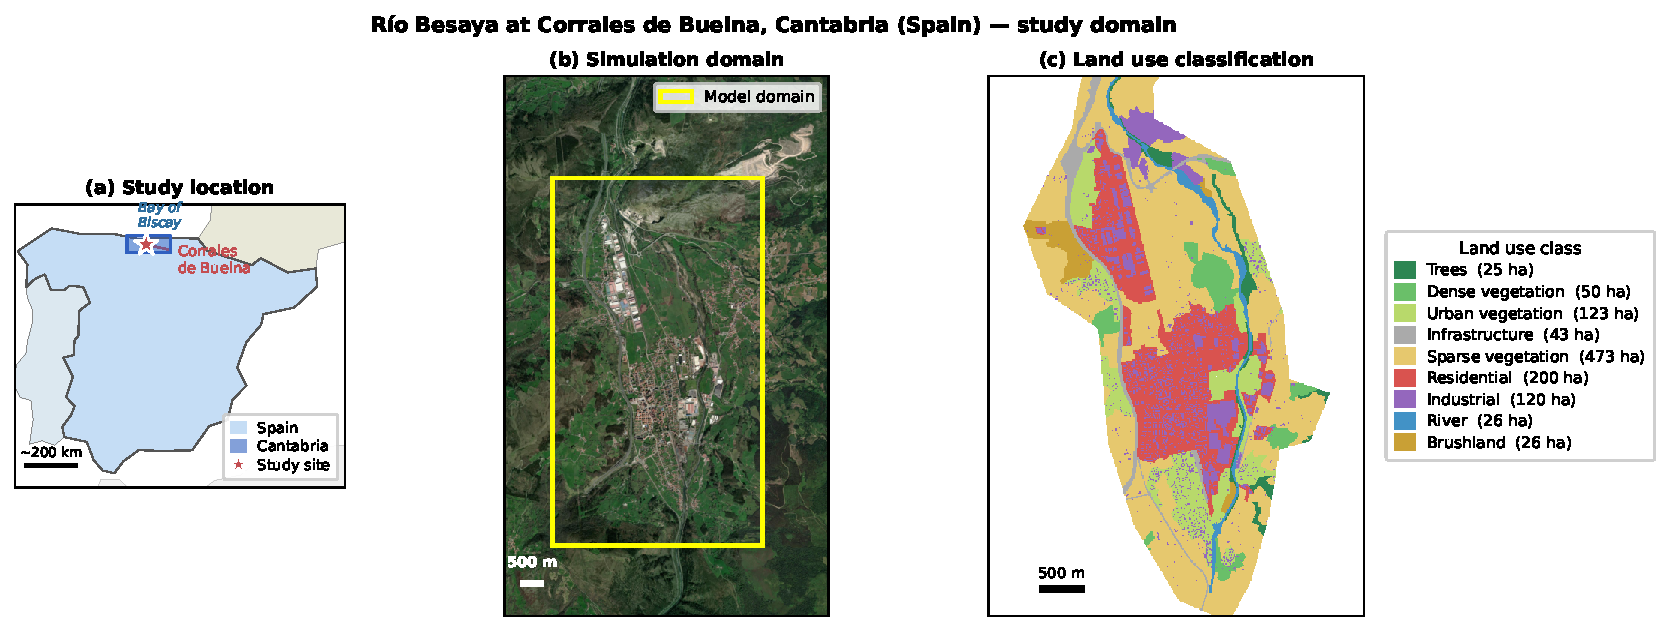
\includegraphics[width=\textwidth]{figures/besaya_fig00_location_map.pdf}
  \caption{Localización del área de estudio del río Besaya en Los Corrales de Buelna (Cantabria). Se muestran el tramo de análisis en la llanura de inundación, las secciones de aforo empleadas y el dominio de la malla hidráulica. Fuente: \parencite{navas2025roughness}.}
  \label{fig:besaya_localizacion}
\end{figure}

Este fue el caso inicial de la línea de investigación y el origen conceptual de \hydra. El trabajo de 2018 planteó, en el contexto de la línea de investigación, la cadena completa que desplaza el período de retorno desde el forzamiento hacia el impacto: generar muchos eventos hidrológicamente plausibles, propagarlos por modelos hidrológicos e hidráulicos y estimar la frecuencia sobre los calados y extensiones resultantes. La necesidad de repetir de forma consistente la preparación de entradas, las ejecuciones y el postprocesado reveló desde el inicio que el principal obstáculo no era un algoritmo aislado, sino la ausencia de una infraestructura reproducible que conectase todas las etapas.

\subsection{Metodología aplicada}

A diferencia del caso Mallorca, la aplicación inicial del Besaya parte de series de aforo. A partir de los registros de caudal se extraen eventos independientes y se caracterizan mediante caudal pico ($Q_p$), duración y volumen. Esta representación multivariante se eligió porque dos avenidas con el mismo pico pueden producir impactos distintos si difieren en volumen o persistencia; asignar toda la frecuencia al pico ocultaría esa diferencia.

La dependencia entre las tres variables se modela con una cópula gaussiana, con marginales ajustadas individualmente. El muestreo amplía el registro observado con eventos sintéticos que conservan combinaciones plausibles de pico, duración y volumen. En el trabajo de 2018, los hidrogramas de diseño se transformaron en manchas y calados mediante Iber, que fue el motor hidráulico empleado en la publicación de la \textit{Revista de Obras Públicas} \parencite{navas2018besaya}. La automatización de HEC-RAS aparece en trabajos posteriores, especialmente en Calle 30 y en el análisis de sensibilidad hidráulica desarrollado posteriormente sobre el mismo dominio.

Cada bloque responde a una limitación concreta y después se generaliza en \hydra: \texttt{climate.time\_series} estandariza la extracción de eventos; \texttt{spatial\_analysis.copulas} evita combinaciones multivariantes incoherentes; los adaptadores de modelos reducen la edición manual entre ejecuciones; y \texttt{hybrid\_downscaling} reduce el coste mediante selección por máxima disimilitud y reconstrucción k-NN. El producto final no es un único mapa determinista, sino una distribución de calado por celda a partir de la que se calculan niveles de retorno.

\begin{figure}[!htbp]
\centering
\resizebox{\textwidth}{!}{%
\begin{tikzpicture}[
  font=\scriptsize,
  proc/.style={
    rectangle, rounded corners=5pt,
    minimum width=2.9cm, minimum height=0.92cm,
    text width=2.65cm, align=center,
    draw=#1!60!black, fill=#1!11,
    line width=0.65pt
  },
  data/.style={
    rectangle, rounded corners=5pt,
    minimum width=2.75cm, minimum height=0.78cm,
    text width=2.5cm, align=center,
    draw=blueblock!65!black, fill=blueblock!10,
    line width=0.6pt
  },
  terrain/.style={
    rectangle, rounded corners=5pt,
    minimum width=2.75cm, minimum height=0.78cm,
    text width=2.5cm, align=center,
    draw=orangeblock!70!black, fill=orangeblock!14,
    line width=0.6pt
  },
  result/.style={
    rectangle, rounded corners=5pt,
    minimum width=3.05cm, minimum height=0.92cm,
    text width=2.8cm, align=center,
    draw=redstep!65!black, fill=redstep!11,
    line width=0.65pt
  },
  arr/.style={-Stealth, line width=0.8pt, color=tg55}
]
\node[data] (qobs) at (0,2.55) {\textbf{Aforos}\\caudal observado};
\node[proc=tealblock] (events) at (3.45,2.55) {\textbf{Eventos}\\pico, volumen, duración};
\node[proc=tealblock] (cop) at (6.9,2.55) {\textbf{Cópula}\\dependencia multivariante};
\node[proc=tealblock] (syntq) at (10.35,2.55) {\textbf{Hidrogramas}\\ensemble sintético};

\node[terrain] (lidar) at (0,0.25) {\textbf{Terreno}\\LiDAR, MDT, usos};
\node[terrain] (mesh) at (3.45,0.25) {\textbf{Iber}\\geometría y rugosidad};
\node[proc=orangeblock] (select) at (6.9,0.25) {\textbf{MaxDiss}\\casos simulados};
\node[proc=orangeblock] (hyd) at (10.35,0.25) {\textbf{Hidráulica}\\calado y velocidad};

\node[result] (impact) at (6.9,-1.95) {\textbf{Impacto}\\distribución por celda};
\node[result] (rp) at (10.35,-1.95) {\textbf{Riesgo}\\retorno del impacto};

\draw[arr] (qobs) -- (events);
\draw[arr] (events) -- (cop);
\draw[arr] (cop) -- (syntq);
\draw[arr] (syntq.south) -- (hyd.north);
\draw[arr] (lidar) -- (mesh);
\draw[arr] (mesh) -- (select);
\draw[arr] (select) -- (hyd);
\coordinate (besayaHydOut) at (10.35,-0.95);
\coordinate (besayaImpactIn) at (6.9,-0.95);
\draw[arr] (hyd.south) -- (besayaHydOut) -- (besayaImpactIn) -- (impact.north);
\draw[arr] (impact) -- (rp);
\end{tikzpicture}
}
\caption{Esquema metodológico de la aplicación fundacional del Besaya--Los Corrales de Buelna \parencite{navas2018besaya}. El flujo parte de eventos de caudal observados, genera hidrogramas sintéticos multivariantes y calcula la frecuencia sobre los impactos hidráulicos simulados con Iber. Esta lógica es el antecedente directo de los módulos de eventos, cópulas, selección de escenarios y postprocesado de impacto de \hydra.}
\label{fig:besaya_esquema_caudal}
\end{figure}

\subsection{Evolución del caso y evidencia reproducible}

El caso ha seguido siendo objeto de investigación tras la aplicación fundacional. Un análisis posterior sobre el mismo dominio \parencite{navas2025roughness} estudia 1.000 combinaciones de rugosidad de Manning con SFINCS y HEC-RAS. Los notebooks empleados en ese trabajo se conservan como material interno para elaborar el artículo y sus figuras; no forman parte del catálogo de ejemplos de uso de \hydra. De las 1.000 combinaciones, 995 simulaciones emparejadas se emplean en la comparación final.

\begin{figure}[htbp]
  \centering
  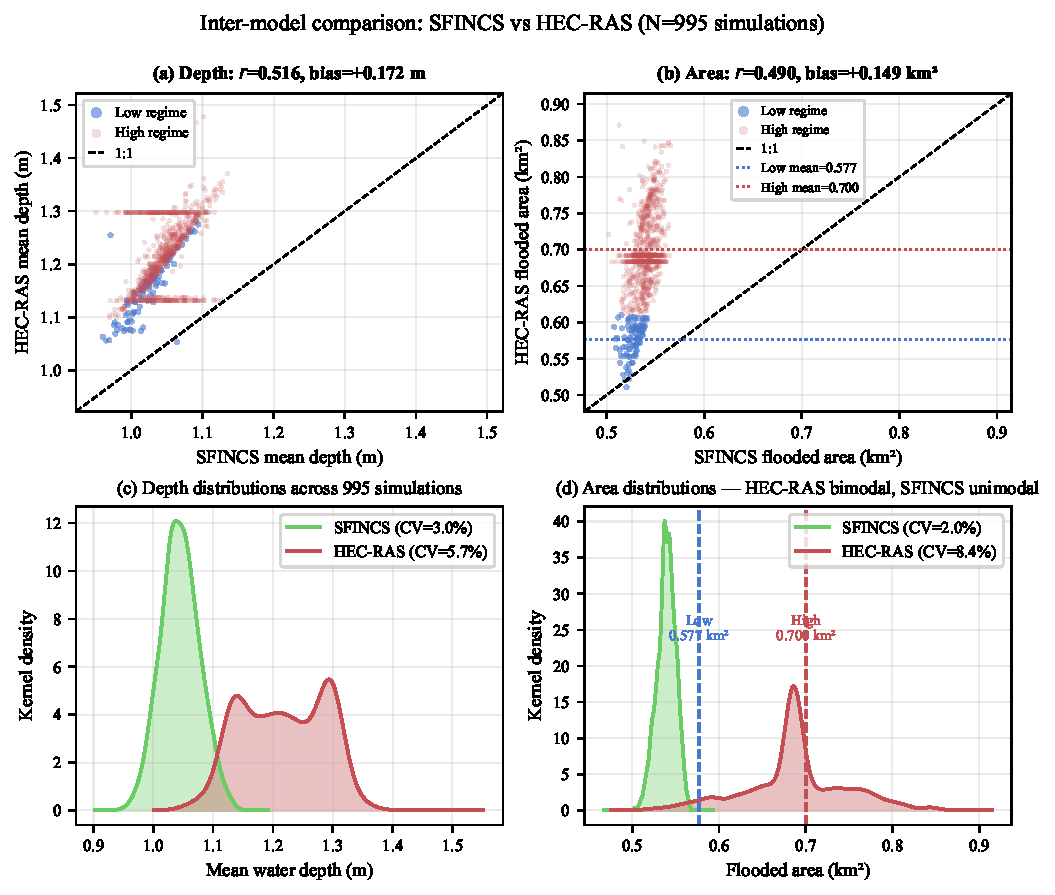
\includegraphics[width=\textwidth]{figures/besaya_fig04_intermodel_comparison.pdf}
  \caption{Comparación de 995 simulaciones emparejadas de SFINCS y HEC-RAS en Los Corrales de Buelna. HEC-RAS produce mayor calado medio y área inundada y presenta una respuesta bimodal que no aparece en SFINCS. Fuente: \parencite{navas2025roughness}.}
  \label{fig:besaya_intermodel}
\end{figure}

La \cref{fig:besaya_intermodel} muestra por qué la automatización masiva no es solo una mejora operativa. La variabilidad entre formulaciones hidráulicas supera la variabilidad atribuible a Manning: HEC-RAS presenta un sesgo medio de $+0{,}172$~m en calado y $+0{,}149$~km\textsuperscript{2} en área respecto a SFINCS, mientras que la correlación entre simulaciones emparejadas es moderada ($r=0{,}52$ para calado y $r=0{,}49$ para área). Una única ejecución no habría permitido identificar esa estructura.

\begin{figure}[htbp]
  \centering
  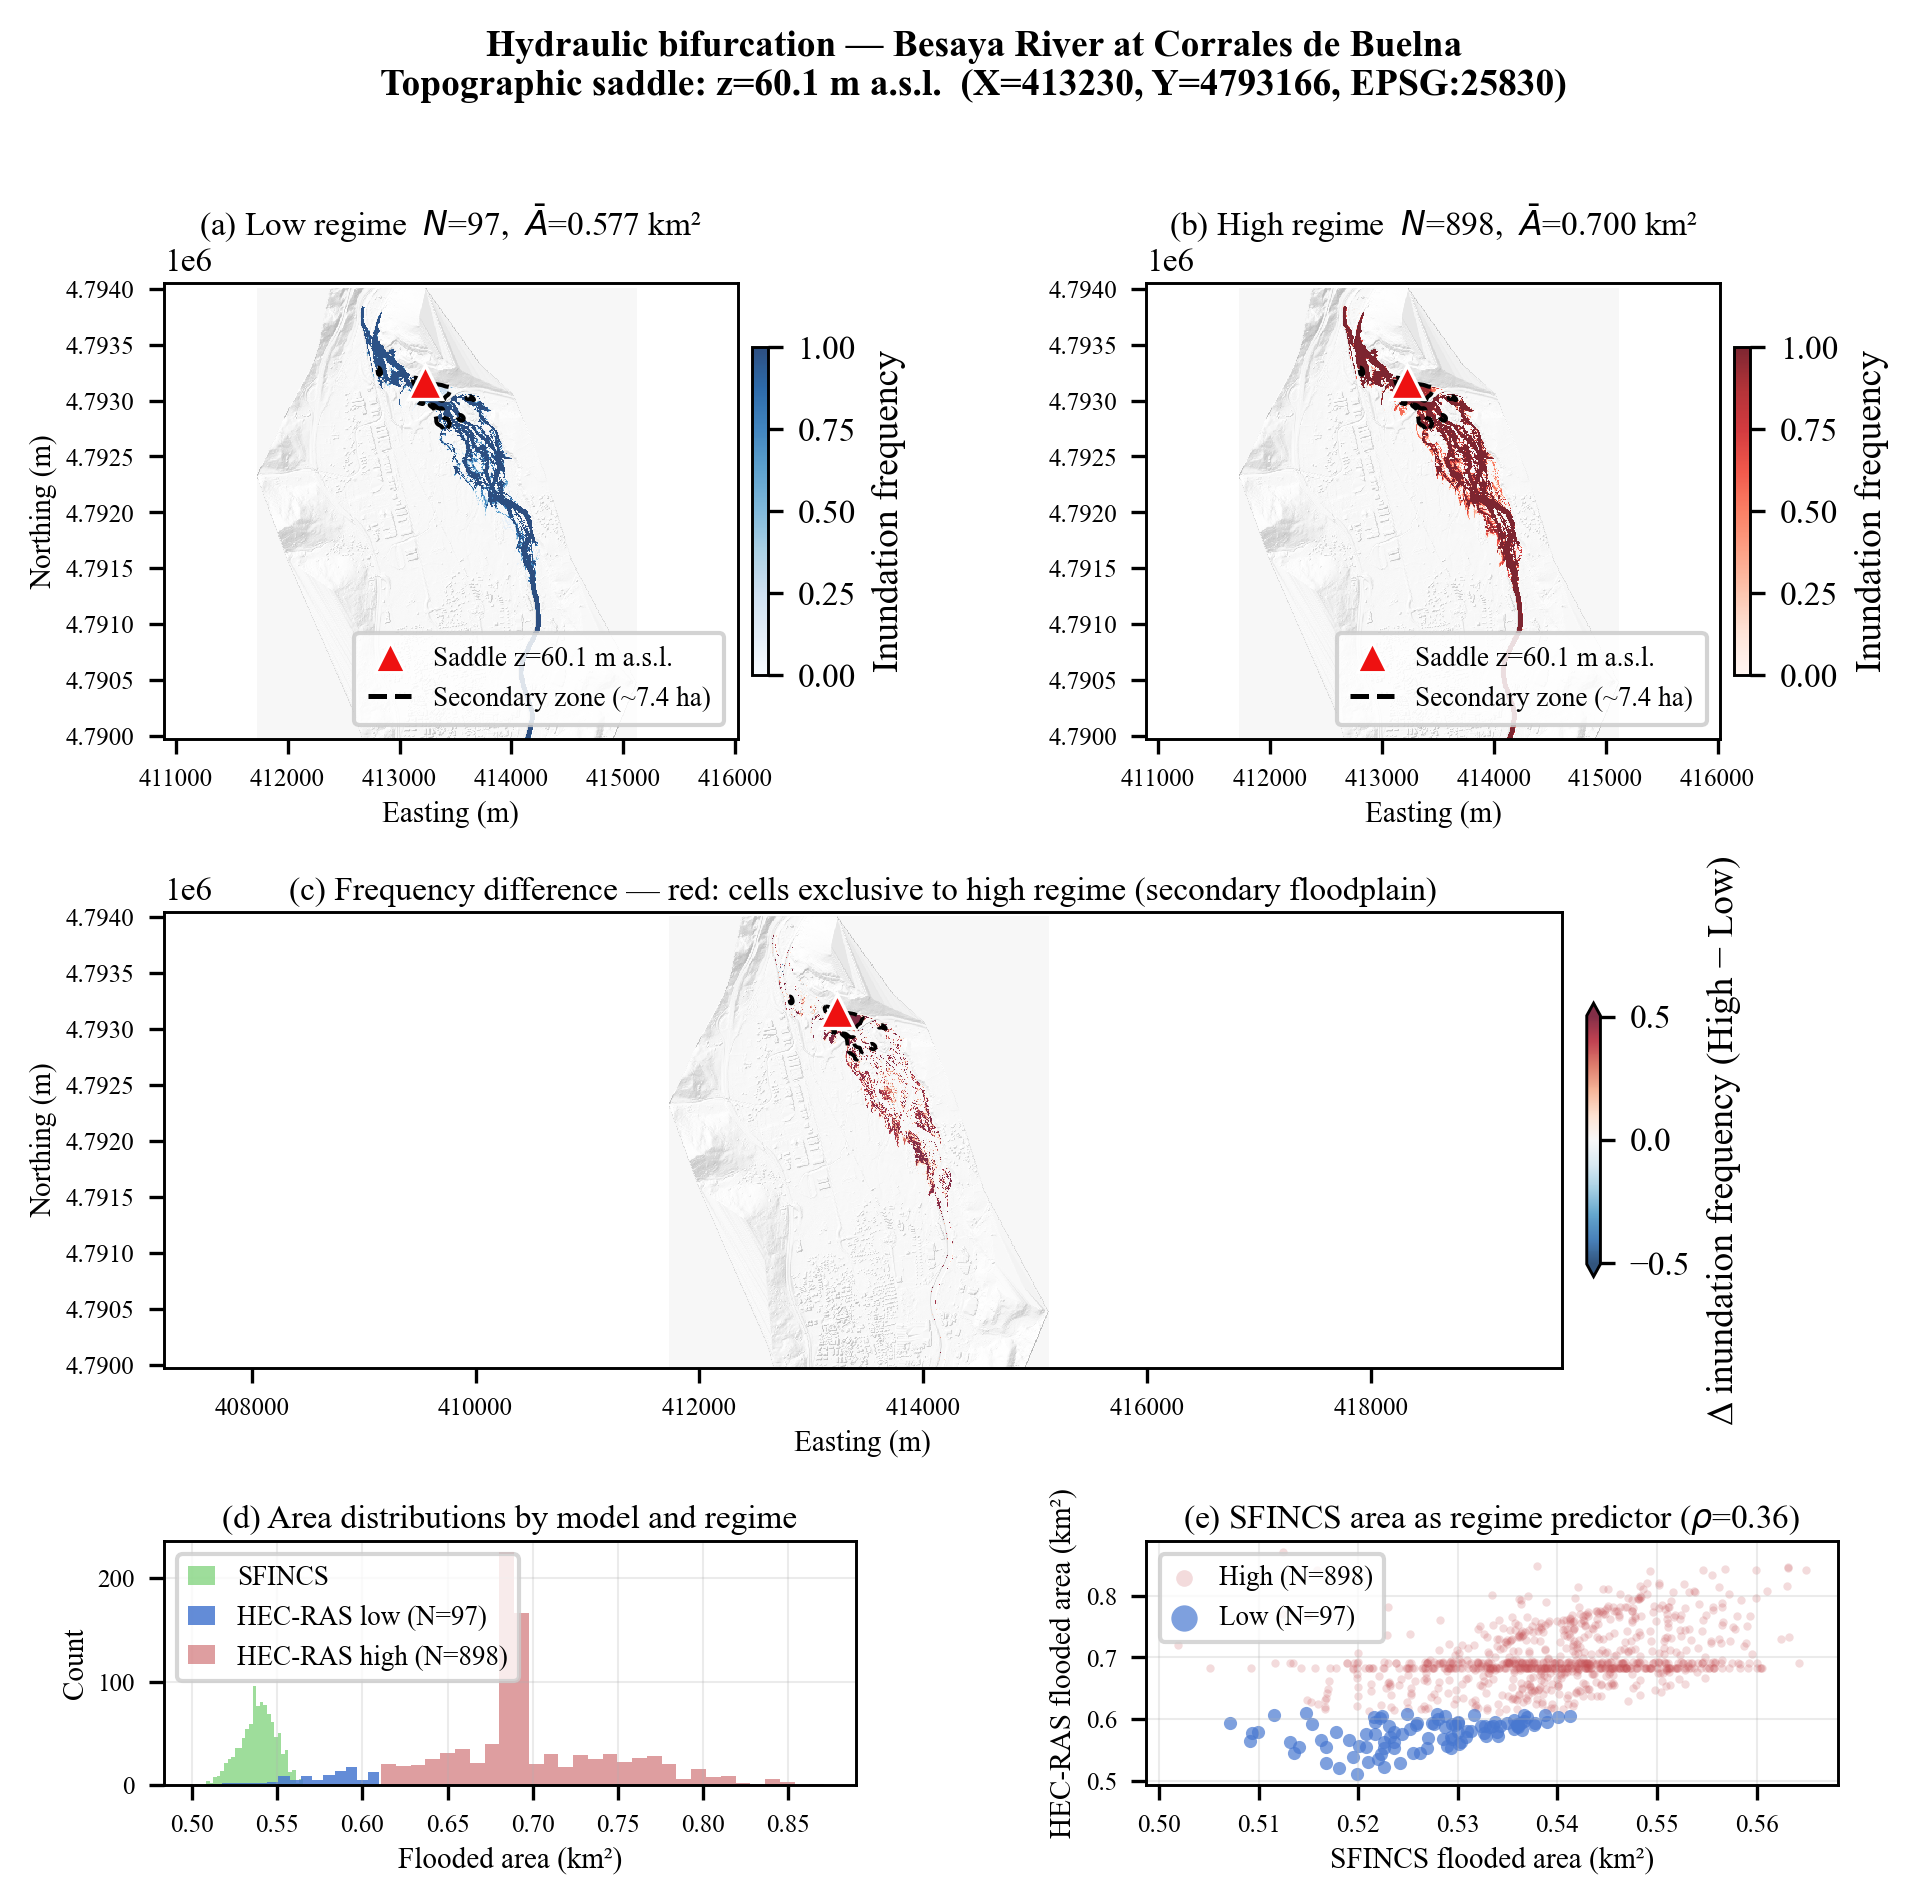
\includegraphics[width=0.95\textwidth]{figures/besaya_fig05_hydraulic_bifurcation.png}
  \caption{Bifurcación hidráulica identificada mediante el ensemble de HEC-RAS. El rebase de un umbral topográfico de aproximadamente 60,1~m activa una llanura secundaria de unas 7,4~ha y separa dos regímenes de área inundada. Fuente: \parencite{navas2025roughness}.}
  \label{fig:besaya_bifurcacion}
\end{figure}

La bifurcación de la \cref{fig:besaya_bifurcacion} evidencia otra aportación de \hydra: conservar salidas espaciales y metadatos de cada ejecución permite pasar de observar una dispersión estadística a explicar su mecanismo físico. Ninguna clase individual de Manning predice el régimen; la transición aparece cuando la dinámica resuelta por HEC-RAS supera un umbral topográfico y conecta una llanura secundaria. Por tanto, el caso valida simultáneamente la cadena estocástica inicial, la ejecución masiva de modelos alternativos y el postprocesado espacial necesario para diagnosticar incertidumbre estructural.

\begin{figure}[htbp]
  \centering
  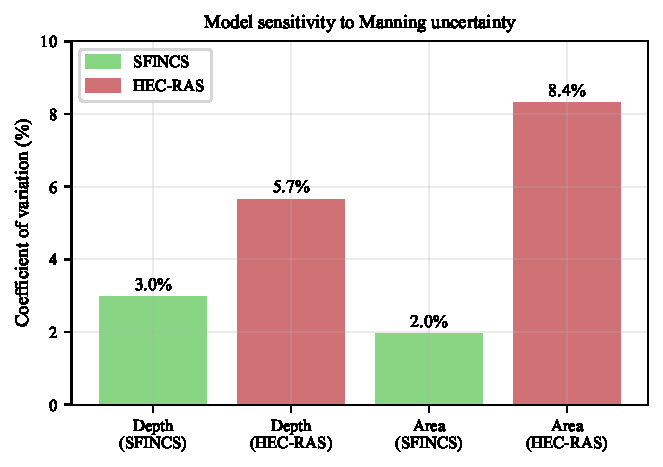
\includegraphics[width=\textwidth]{figures/besaya_fig06_cv_comparison.pdf}
  \caption{Comparación de la variabilidad de calado y área inundada entre SFINCS y HEC-RAS mediante validación cruzada en Los Corrales de Buelna. Los paneles muestran la distribución de los coeficientes de variación para ambas métricas de impacto, desagregados por clase de rugosidad de Manning. La variabilidad intermodelo supera sistemáticamente la variabilidad intramodelo atribuible a Manning. Fuente: \parencite{navas2025roughness}.}
  \label{fig:besaya_cv_comparison}
\end{figure}

\begin{figure}[htbp]
  \centering
  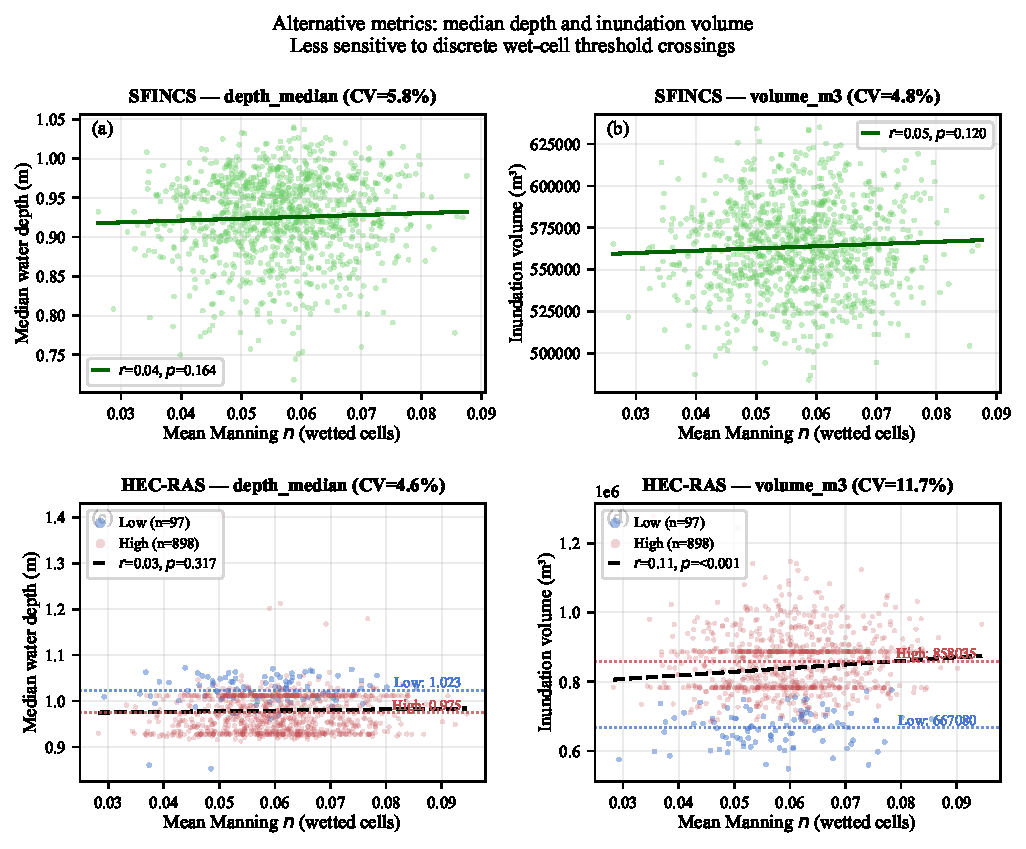
\includegraphics[width=\textwidth]{figures/besaya_fig07_alternative_metrics.pdf}
  \caption{Métricas alternativas de sensibilidad hidráulica en el ensemble de 995 simulaciones emparejadas SFINCS--HEC-RAS. Los paneles muestran índices de concordancia, errores porcentuales y métricas de superposición espacial entre los resultados de ambos modelos. La independencia de las conclusiones respecto a la métrica empleada refuerza la robustez del análisis. Fuente: \parencite{navas2025roughness}.}
  \label{fig:besaya_alternative_metrics}
\end{figure}


\clearpage
\section{Sant Llorenç des Cardassar, Mallorca}
\label{sec:caso_mallorca}

\subsection{Contexto y problema}

El 9 de octubre de 2018 una intensa precipitación convectiva causó el desbordamiento del torrente Ses Planes en la localidad de Sant Llorenç des Cardassar (Mallorca). El episodio acumuló alrededor de 220 litros por metro cuadrado en pocas horas, generando una avenida rápida que provocó pérdidas humanas y daños materiales de gran magnitud. La cuenca del torrente Ses Planes es un ejemplo representativo de régimen hidrológico torrencial mediterráneo: tiempos de concentración inferiores a una hora, pendientes pronunciadas y ausencia de registros de aforo en la sección de interés.

El reto metodológico de este caso es doble. Primero, la generación de escenarios de precipitación plausibles a partir de series pluviométricas cortas y escasas estaciones. Segundo, la obtención de mapas de inundación asociados a períodos de retorno en una cuenca sin calibración de caudal, utilizando como única referencia la mancha de inundación del evento histórico registrada por el servicio Copernicus \parencite{navas2019mallorca}.

\subsection{Metodología aplicada}

La cadena metodológica de este caso arranca desde los pluviómetros horarios del SIAR disponibles en la zona y se complementa con productos satelitales de precipitación. En particular, se utilizó PERSIANN como fuente independiente para contrastar la representatividad espacial de los registros puntuales y para analizar la estructura de la lluvia en el entorno de la cuenca \parencite{ashouri2015persiann}. El notebook interno \texttt{Reconstrucción Precipitación.ipynb} documenta esta fase de trabajo: lectura de SIAR, extracción de celdas PERSIANN, comparación estación-satélite, contraste con TRMM y reconstrucción espacial de la lluvia mediante interpolación geoestadística.

Aunque PERSIANN y TRMM aportaron una referencia espacial externa, no se adoptaron como forzamiento final del modelo hidrológico. La resolución espacial, los sesgos respecto a los pluviómetros horarios y la dificultad para reproducir la estructura local de un episodio convectivo rápido hicieron preferible reconstruir la lluvia con kriging a partir de la red observada. Esta decisión es metodológicamente importante: el caso Mallorca no valida simplemente el uso de datos satelitales, sino la primera formulación de un downscaling híbrido desde precipitación en la línea de investigación, donde los productos remotos sirven para diagnóstico y contraste, mientras que el campo final de lluvia se genera mediante reconstrucción geoestadística controlada por observaciones.

Los eventos de precipitación se detectan y caracterizan mediante cuatro parámetros: precipitación máxima horaria ($P_{max}$), precipitación media del evento ($P_{med}$), duración total y forma del hietograma. Para la clasificación de formas de hietograma se aplica un análisis de componentes principales seguido de K-means, que agrupa los hietogramas históricos en 25 tipos representativos.

A partir de los eventos históricos clasificados se construye un modelo de cópulas gaussianas en \texttt{pyhydra.climate.spatial\_analysis} que preserva la dependencia entre $P_{max}$, $P_{med}$, duración y tipo de hietograma en cada pluviómetro, y la dependencia espacial entre estaciones. Mediante muestreo de la cópula se generan miles de eventos sintéticos que amplían el espacio de escenarios plausibles más allá de los registros históricos disponibles.

De este conjunto se seleccionan los escenarios más representativos mediante el algoritmo de máxima disimilitud en \texttt{pyhydra.climate.hybrid\_downscaling}, reduciendo el número de simulaciones completas a ejecutar. Para cada evento seleccionado se reconstruye el campo de precipitación distribuida sobre la cuenca mediante kriging universal con la elevación como variable de tendencia, produciendo rasters horarios a 25 metros de resolución que se introducen en el módulo hidrológico del modelo Iber. La \cref{fig:mallorca_reconstruccion_lluvia} muestra un ejemplo de reconstrucción horaria del episodio del 9 de octubre de 2018 empleado como referencia para comprobar la coherencia espacio-temporal de los campos de lluvia.

\begin{figure}[htbp]
  \centering
  \begin{tikzpicture}
    \node[inner sep=0] (img) {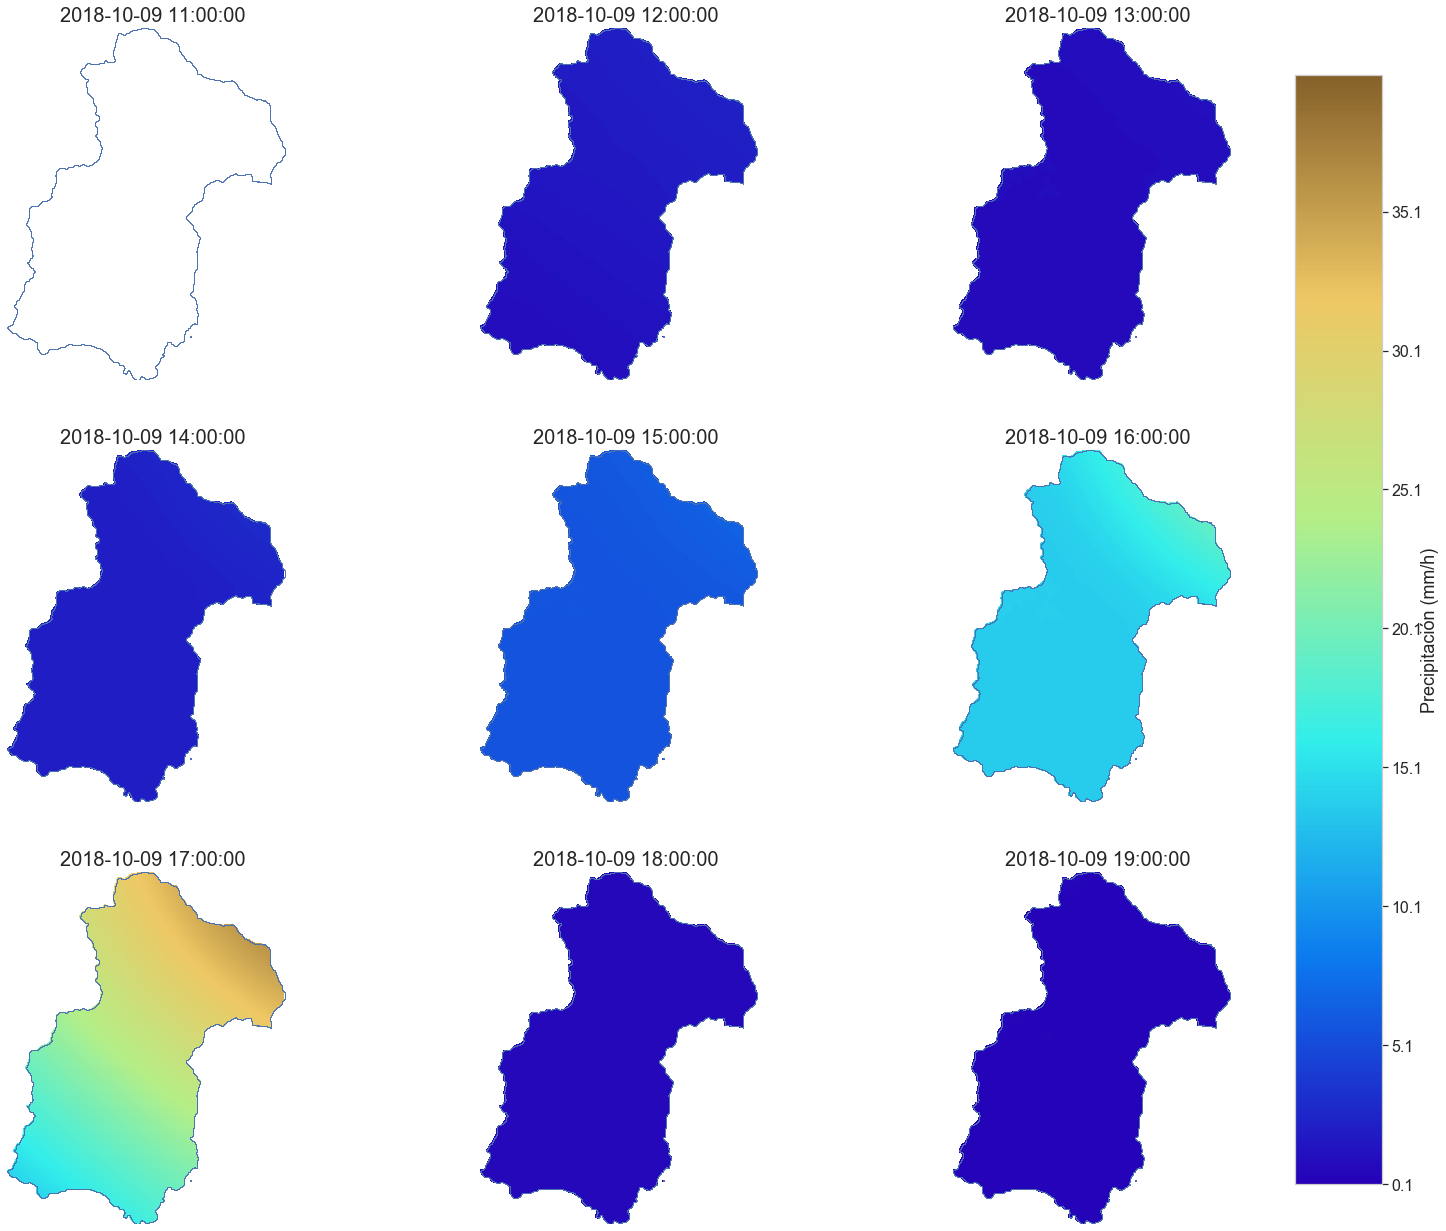
\includegraphics[width=0.94\textwidth]{figures/fig_mallorca_reconstruccion_lluvia.png}};
    \node[font=\small, align=center] at ([yshift=-0.45cm]img.south) {Coordenada horizontal aproximada / longitud};
    \node[font=\small, rotate=90, align=center] at ([xshift=-0.35cm]img.west) {Coordenada vertical aproximada / latitud};
    \node[font=\small, align=center] at ([yshift=0.35cm]img.north) {Campo horario reconstruido mediante kriging};
  \end{tikzpicture}
  \caption{Reconstrucción horaria de la precipitación sobre la cuenca de Sant Llorenç des Cardassar durante el episodio del 9 de octubre de 2018. La figura procede del notebook interno de reconstrucción de precipitación utilizado en el trabajo de Mallorca; se han añadido rótulos editoriales sobre la imagen exportada para mejorar su lectura. Resume la fase de interpolación espacial previa a la simulación hidrológica distribuida.}
  \label{fig:mallorca_reconstruccion_lluvia}
\end{figure}

La simulación hidrológica e hidráulica se realiza en dos fases. La fase hidrológica utiliza la malla de la cuenca completa (MDT 25 m) para transformar la precipitación distribuida en caudales en la sección de entrada a la localidad. La fase hidráulica emplea una malla de mayor resolución (triángulos de 8 m) construida a partir del LiDAR-PNOA del IGN, con los hidrogramas obtenidos de la fase anterior como condición de contorno. La calibración iterativa ajusta los parámetros de infiltración hasta reproducir la mancha de inundación Copernicus del 9 de octubre de 2018, obteniendo calados máximos simulados de hasta 5,85 m en el casco urbano.

Para el conjunto de eventos sintéticos no simulados completamente, los calados y velocidades se reconstruyen mediante k-NN con 6 vecinos, valor óptimo determinado minimizando el error acumulado sobre los 10 últimos eventos simulados de la base de referencia. El resultado final es la distribución empírica de calados en cada celda de la malla hidráulica, con la que se calculan los mapas de período de retorno basados en impacto hidráulico.

\subsection{Resultados y conexión con HYDRA}

El caso Mallorca valida la primera implementación de la cadena de downscaling híbrido basada en precipitación: integración de registros horarios, análisis diagnóstico de precipitación satelital PERSIANN y TRMM, generación de eventos multivariantes con cópulas gaussianas, selección por máxima disimilitud, reconstrucción espacial de campos de lluvia mediante kriging, simulación hidrológica e hidráulica, y reconstrucción de manchas de inundación por k-NN. Es el primer caso en el que la estadística de extremos se aplica sobre variables hidráulicas en lugar de sobre la precipitación forzante, lo que constituye una diferencia metodológica central con los enfoques convencionales.

La comparación entre la mancha simulada para el evento del 9 de octubre de 2018 y la cartografía Copernicus confirma la coherencia del modelo calibrado. La disponibilidad de esa referencia externa independiente es lo que hace de este caso un banco de pruebas válido para la metodología estocástica. Debe precisarse el alcance de esa comparación: la delineación rápida de Copernicus EMS es una referencia de extensión, no de calado, y presenta limitaciones conocidas en zona urbana (sombras de edificación, momento de adquisición posterior al pico de la avenida), por lo que la calibración se evaluó como coherencia de extensión y de niveles máximos en puntos con marcas de avenida documentadas, y no mediante índices de acierto celda a celda. La sistematización de métricas cuantitativas de contraste (índice de acierto crítico sobre la extensión, error de calado en marcas de avenida) sobre este tipo de referencias post-evento forma parte del protocolo de validación descrito en la \cref{sec:validacion_knn} y es directamente aplicable cuando se disponga de levantamientos de campo con calidad suficiente.

\begin{figure}[htbp]
  \centering
  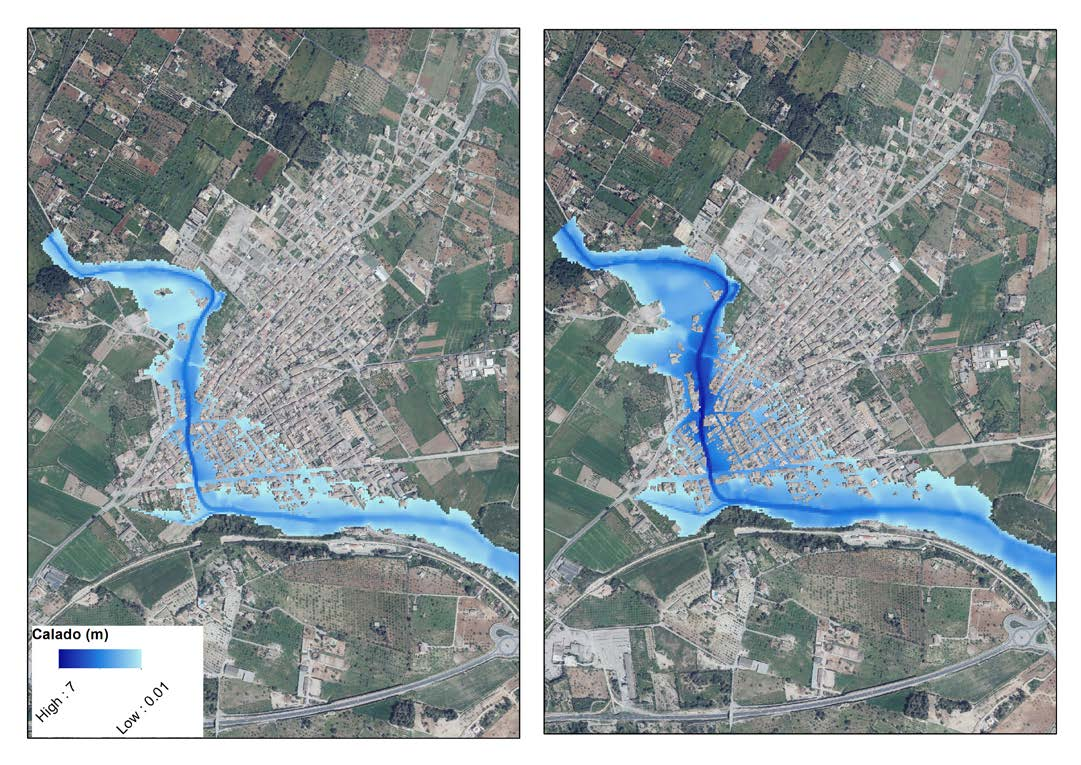
\includegraphics[width=\textwidth]{figures/fig_mallorca_comparativa.png}
  \caption{Comparación de las manchas y calados obtenidos para Sant Llorenç des Cardassar mediante dos formas de caracterizar los eventos de diseño. La aplicación estocástica (derecha) explora una extensión y una distribución de calados diferentes de la obtenida con la metodología habitual (izquierda), ilustrando la importancia de calcular la frecuencia sobre la variable hidráulica final. Fuente: comunicación presentada en las VI Jornadas de Ingeniería del Agua \parencite{navas2019mallorca}.}
  \label{fig:mallorca_calado}
\end{figure}

\clearpage
\section{Calle 30, Madrid}
\label{sec:caso_madrid}

\subsection{Contexto y problema}

La Calle 30 agrupa las infraestructuras soterradas y elevadas de la M-30 en el entorno del río Manzanares en Madrid. Su exposición al riesgo de inundación combina la escorrentía de cuencas externas de mediano tamaño, la precipitación directa y la posibilidad de interacciones con el nivel freático. La complejidad del sistema hidrológico y la importancia de la infraestructura como eje de movilidad metropolitana exigen metodologías capaces de explorar un espacio amplio de escenarios de forzamiento. El caso se presentó inicialmente en las VII Jornadas de Ingeniería del Agua \parencite{deljesus2023calle30} y fue desarrollado posteriormente como artículo \parencite{navas2024calle30,deljesus2024downscaling}.

\begin{figure}[htbp]
  \centering
  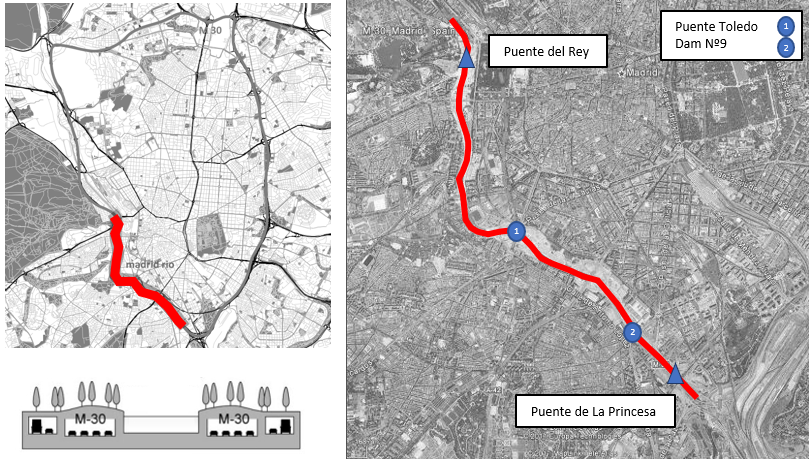
\includegraphics[width=\textwidth]{figures/fig_m30_localizacion}
  \caption{Localización del área de estudio del sistema de infraestructuras Calle 30 -- M-30 en Madrid. El recuadro superior muestra la situación en la Comunidad de Madrid; el inferior delimita el tramo soterrado y las cuencas contribuyentes instrumentadas. Elaboración propia, publicada en \parencite{navas2024calle30}.}
  \label{fig:m30_localizacion}
\end{figure}

\subsection{Metodología aplicada}

La cadena metodológica de Calle 30 es la más completa de los casos aplicados hasta la fecha. Comienza con la descarga y procesamiento de precipitación ERA5 \parencite{hersbach2020era5} y datos pluviométricos de AEMET mediante \texttt{pyhydra.data\_sources.rainfall}. El análisis estadístico de extremos de precipitación multiduracion con GEV en \texttt{pyhydra.climate.time\_series} proporciona las distribuciones de referencia para los forzamientos de diseño.

Los eventos sintéticos se generan mediante cópulas gaussianas multivariantes que modelizan la dependencia entre duraciones y volúmenes de precipitación en las subcuencas contribuyentes. La simulación hidrológica con HEC-HMS produce series de caudales en las secciones de entrada al sistema de drenaje de la M-30. Sobre estas series se aplica la selección de escenarios representativos por máxima disimilitud, seguida de simulación hidráulica completa con HEC-RAS 1D para los escenarios seleccionados. Para el resto, los calados se reconstruyen mediante downscaling híbrido con k-NN \parencite{deljesus2024downscaling}.

El resultado final son mapas de período de retorno basados en calado hidráulico obtenidos con \texttt{pixel\_return\_period} de \texttt{pyhydra.climate.hybrid\_downscaling}, que expresan para cada celda del dominio hidráulico la probabilidad de excedencia anual del calado calculado.

\begin{figure}[!htbp]
\centering
\resizebox{0.98\textwidth}{!}{%
\begin{tikzpicture}[
  font=\scriptsize,
  stat/.style={
    rectangle, rounded corners=5pt,
    minimum width=3.35cm, minimum height=1.15cm,
    text width=3.0cm, align=center,
    draw=tealblock!60!black, fill=tealblock!11,
    line width=0.65pt
  },
  dyn/.style={
    rectangle, rounded corners=5pt,
    minimum width=3.35cm, minimum height=1.15cm,
    text width=3.0cm, align=center,
    draw=orangeblock!70!black, fill=orangeblock!14,
    line width=0.65pt
  },
  hyd/.style={
    rectangle, rounded corners=5pt,
    minimum width=3.35cm, minimum height=1.15cm,
    text width=3.0cm, align=center,
    draw=redstep!60!black, fill=redstep!12,
    line width=0.65pt
  },
  data/.style={
    rectangle, rounded corners=5pt,
    minimum width=3.35cm, minimum height=0.95cm,
    text width=3.0cm, align=center,
    draw=blueblock!65!black, fill=blueblock!10,
    line width=0.6pt
  },
  note/.style={
    rectangle, rounded corners=4pt,
    minimum width=2.9cm, minimum height=0.65cm,
    text width=2.65cm, align=center,
    draw=tg40, fill=tg5,
    line width=0.5pt, font=\scriptsize
  },
  arr/.style={-Stealth, line width=0.8pt, color=tg55}
]
\node[data] (rain) at (0,3.2) {\textbf{Precipitación}\\ERA5 + pluviómetros};
\node[stat] (sep) at (3.95,3.2) {\textbf{Eventos de lluvia}\\duración, volumen, intensidad};
\node[stat] (cop) at (7.9,3.2) {\textbf{Cópulas multivariantes}\\dependencia espacial y temporal};
\node[stat] (synt) at (11.85,3.2) {\textbf{Eventos sintéticos}\\precipitación en subcuencas};


\node[stat] (selecthms) at (11.85,1.35) {\textbf{Selección inicial}\\escenarios para HEC-HMS};
\node[dyn] (hms) at (7.9,1.35) {\textbf{Simulación hidrológica}\\HEC-HMS};
\node[stat] (maxdiss) at (3.95,1.35) {\textbf{Selección hidráulica}\\MaxDiss sobre hidrogramas};

\node[data] (terrain) at (0,-0.75) {\textbf{Modelo urbano}\\MDT, drenaje, geometría};
\node[hyd] (ras) at (3.95,-0.75) {\textbf{Simulación hidráulica}\\HEC-RAS 1D};
\node[stat] (knn) at (7.9,-0.75) {\textbf{Reconstrucción k-NN}\\mapas no simulados};
\node[hyd] (rp) at (11.85,-0.75) {\textbf{Períodos de retorno}\\calado por pixel};

\draw[arr] (rain) -- (sep);
\draw[arr] (sep) -- (cop);
\draw[arr] (cop) -- (synt);
\draw[arr] (synt.south) -- (selecthms.north);
\draw[arr] (selecthms.west) -- (hms.east);
\draw[arr] (hms.west) -- (maxdiss.east);
\coordinate (m30MaxOut) at (3.95,0.35);
\draw[arr] (maxdiss.south) -- (m30MaxOut) -- (ras.north);
\draw[arr] (terrain) -- (ras);
\draw[arr] (ras) -- (knn);
\draw[arr] (knn) -- (rp);
\end{tikzpicture}
}
\caption{Esquema metodológico del caso Calle 30--M-30 Madrid \parencite{navas2024calle30,deljesus2024downscaling}. A diferencia del Besaya, el flujo parte de precipitación multisitio: los eventos de lluvia se generan con cópulas, se transforman en caudales con HEC-HMS, se selecciona un subconjunto hidráulicamente representativo con MaxDiss y se simula con HEC-RAS 1D. La reconstrucción k-NN de los resultados no simulados constituye el downscaling híbrido.}
\label{fig:m30_esquema_precipitacion}
\end{figure}

\subsection{Resultados y conexión con HYDRA}

Los resultados del estudio \parencite{navas2024calle30} son mapas de calado asociados a distintos períodos de retorno en el entorno de la M-30 semienterrada. La comparación con evaluaciones previas disponibles para la misma área confirma la coherencia de los resultados y cuantifica la diferencia entre el período de retorno del forzamiento meteorológico y el del impacto hidráulico, que en sistemas urbanos con efectos de atenuación o concentración puede ser significativa.

El caso Calle 30 es la validación de referencia de la Tarea 2 del plan de investigación: la combinación de generación estocástica, máxima disimilitud, simulación hidráulica y reconstrucción k-NN para obtener períodos de retorno basados en variables de impacto. Es el caso sobre el que se ha definido la interfaz entre todos los módulos de \hydra.

\paragraph{Justificación de las herramientas.}
En Calle 30, el uso de \hydra se justifica por la combinación de tres fuentes de complejidad sintetizadas en la \cref{fig:m30_esquema_precipitacion}. Primero, varios pluviómetros y subcuencas producen forzamientos espacialmente dependientes, por lo que las cópulas evitan generar escenarios incompatibles entre puntos. Segundo, cada escenario exige encadenar HEC-HMS y HEC-RAS 1D, de modo que la automatización de entradas y salidas es necesaria para mantener la trazabilidad. Tercero, el coste de HEC-RAS impide simular exhaustivamente el conjunto sintético, lo que hace necesaria la selección MaxDiss y la reconstrucción k-NN. La utilidad de cada módulo queda así vinculada a una necesidad verificable del caso, no solo a la disponibilidad de la herramienta.

\clearpage
\section{Valencia: análisis del episodio DANA de octubre 2024}
\label{sec:caso_valencia}

\subsection{Contexto y problema}

El 29 de octubre de 2024 una depresión aislada en niveles altos (DANA) generó precipitaciones extremas en la Comunidad Valenciana. La estación 8337X en Turís registró 710,8 mm en 24 horas, estableciendo un récord nacional. La estación V103 en Carlet registró 265,1 mm en el mismo período. Ambas estaciones están separadas aproximadamente 21,7 km. El evento causó más de 220 víctimas y daños materiales de magnitud excepcional en el área metropolitana de Valencia.

El problema estadístico que plantea el episodio es la estimación del período de retorno de precipitación extrema de corta duración en una región con alta variabilidad interanual, series pluviométricas de longitud limitada y registros históricos que no habían incluido jamás un evento de esta magnitud. En estas condiciones, los métodos clásicos de estimación muestran una sensibilidad extrema a la inclusión o exclusión del evento en la serie, con estimaciones de período de retorno que varían en órdenes de magnitud dependiendo del enfoque utilizado \parencite{deljesus2025jia}.

\subsection{Metodología aplicada}

El estudio aplica y compara tres métodos de ajuste de la distribución GEV sobre series de máximos anuales de precipitación diaria acumulada en dos niveles de análisis: individual por estación y regional de frecuencia.

El análisis individual se centra en las estaciones 8337X (Turís) y V103 (Carlet). Se ajusta la distribución GEV mediante máxima verosimilitud (MLE), L-momentos y estimación bayesiana con priors débiles mediante MCMC hamiltoniano (4 cadenas, 1000 muestras) con PyMC, siguiendo la estructura del módulo \texttt{pyhydra.climate.time\_series}. Para cada método se comparan dos escenarios: con y sin la inclusión del evento de 2024 en la serie.

El análisis regional de frecuencia se aplica a dos escalas. El RFA local utiliza un grupo de 9 estaciones ubicadas en el entorno de Turís y Carlet, seleccionadas por proximidad espacial y coherencia pluviométrica. El RFA global utiliza una red ampliada de estaciones distribuidas por la Comunidad Valenciana. En ambos casos se emplea el procedimiento de Hosking y Wallis \parencite{hosking1997rfa}: estandarización de series (Z-score por estación), construcción de la muestra regional (máximo anual entre estaciones estandarizadas), y ajuste GEV a la serie regional mediante los tres métodos. La transferencia a escala local se realiza mediante la transformación inversa $z_{T,i} = y_T \cdot s_i + \bar{x}_i$, donde $y_T$ es el cuantil regional adimensional para el período de retorno $T$, y $s_i$ y $\bar{x}_i$ son la desviación típica y la media empíricas de la estación de interés. El conjunto de datos empleado comprende 224 estaciones (30 AEMET, 41 SIAR, 153 AVAMET).

\subsection{Resultados}

Los resultados del análisis individual muestran una sensibilidad extrema de los métodos clásicos a la inclusión del evento. Sin incluir la DANA, el método bayesiano estima para Turís un nivel de precipitación de 260 mm para un período de retorno de 100 años y 417,6 mm para 500 años. Al incluir el evento, las mismas estimaciones ascienden a 952 mm y 3004 mm respectivamente (Tabla~\ref{tab:results_valencia_individual}). Para los L-momentos la variación es menos pronunciada pero mantiene la misma tendencia.

\begin{table}[htbp]
  \centering
  \caption{Niveles de precipitación estimados (mm) para distintos períodos de retorno en Turís y Carlet. Análisis individual. El valor bayesiano se expresa en mm; MLE y L-momentos como porcentaje de cambio respecto al bayesiano.}
  \label{tab:results_valencia_individual}
  \resizebox{\textwidth}{!}{%
  \begin{tabular}{llrrrrrrr}
    \toprule
    & & \multicolumn{3}{c}{Sin considerar DANA} & \multicolumn{3}{c}{Considerando DANA} \\
    \cmidrule(lr){3-5}\cmidrule(lr){6-8}
    Estación & T & Bayes (mm) & MLE (\%) & L-mom (\%) & Bayes (mm) & MLE (\%) & L-mom (\%) \\
    \midrule
    Turís & 10  & 126,0 & -5,5 & -5,1 & 195,2 & -4,9 & -15,3 \\
    (8337X) & 100 & 260,2 & -12,7 & -16,2 & 952,0 & -13,7 & -20,6 \\
           & 500 & 417,6 & -18,6 & -25,3 & 3004,1 & -21,0 & -24,0 \\
    \midrule
    Carlet & 10  & 125,5 & -3,7 & -2,6 & 146,3 & -3,9 & -3,3 \\
    (V103) & 100 & 202,8 & -8,7 & -7,0 & 293,0 & -8,3 & -1,7 \\
           & 500 & 262,2 & -11,9 & -10,1 & 450,5 & -11,9 & -0,3 \\
    \bottomrule
  \end{tabular}}
\end{table}

El período de retorno estimado para los valores observados el 29 de octubre de 2024 (710,8 mm en Turís, 265,1 mm en Carlet) es especialmente revelador. Sin incluir el evento en la serie, los métodos clásicos estiman períodos de retorno superiores a 11.000 años en Turís (MLE) y de más de 31.000 años (L-momentos), mientras que el método bayesiano estima 3.069 años. Al incluir el evento, las estimaciones descienden bruscamente a valores coherentes: entre 66 y 91 años en Turís y entre 70 y 95 años en Carlet (Tabla~\ref{tab:returns_valencia}).

\begin{table}[htbp]
  \centering
  \caption{Períodos de retorno estimados (años) para los valores observados el 29 de octubre de 2024. Análisis individual.}
  \label{tab:returns_valencia}
  \resizebox{0.85\textwidth}{!}{%
  \begin{tabular}{lrrrrrrr}
    \toprule
    & \multicolumn{3}{c}{Sin considerar DANA} & \multicolumn{3}{c}{Considerando DANA} \\
    \cmidrule(lr){2-4}\cmidrule(lr){5-7}
    Estación & Bayes & MLE & L-mom & Bayes & MLE & L-mom \\
    \midrule
    Turís (710,8 mm)  & 3069 & 11453 & 31345 & 66 & 80 & 91 \\
    Carlet (265,1 mm) & 536  & 1616  & 1329  & 70 & 95 & 75 \\
    \bottomrule
  \end{tabular}}
\end{table}

El análisis RFA local (9 estaciones próximas) produce estimaciones más estables que el análisis individual: el período de retorno del evento en Turís, sin incluir la DANA, se estima entre 581.741 y 7.549.328 años (valores sin sentido práctico), mientras que al incluirlo desciende a 34-41 años. El RFA global tiende a suavizar los efectos del evento extremo, produciendo períodos de retorno de 10-19 años en Turís con la DANA incluida.

\begin{figure}[htbp]
  \centering
  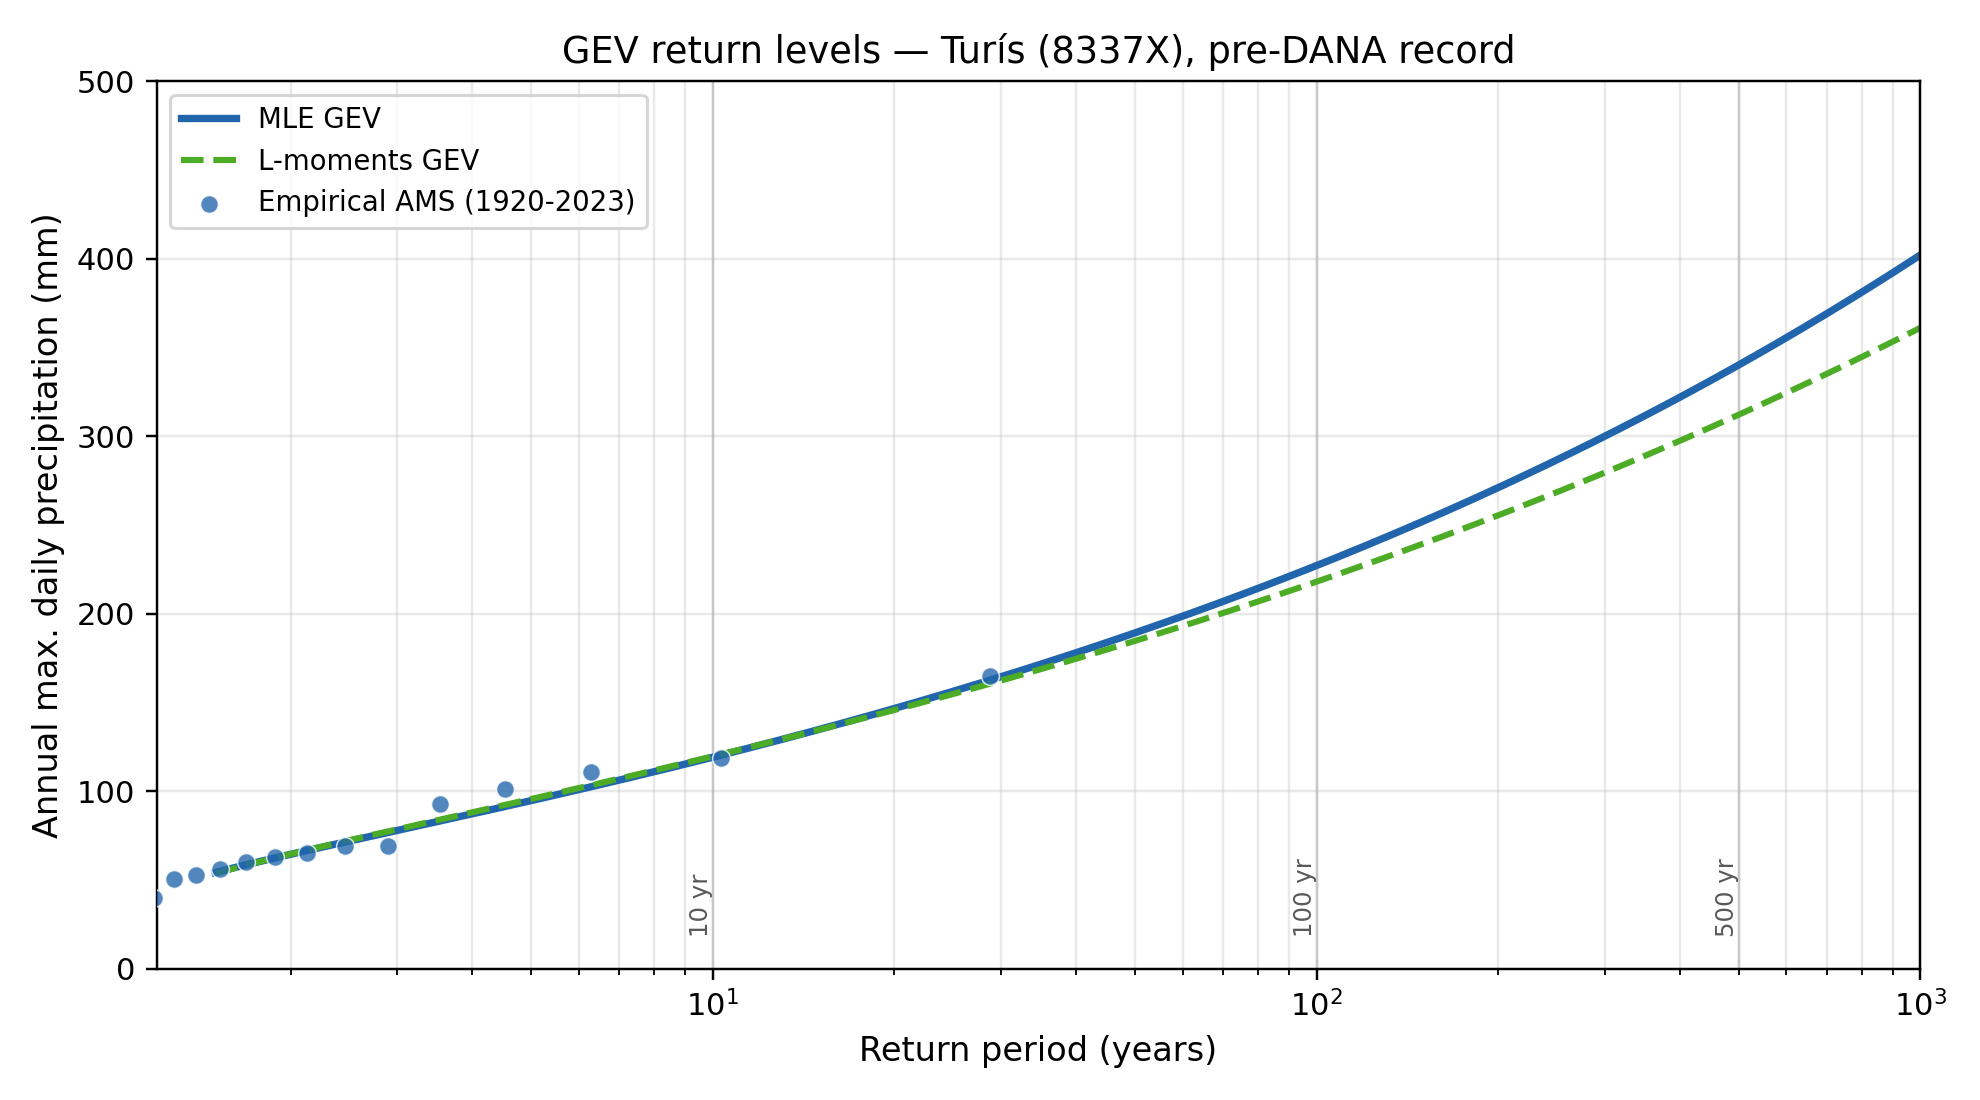
\includegraphics[width=\linewidth]{figures/fig_valencia_curvas_retorno_pre_dana_notebook.png}
  \caption[Curvas de nivel de retorno GEV pre-DANA en Turís]{Curvas de nivel de retorno GEV para la estación 8337X (Turís), obtenidas con la serie de máximos anuales previa al episodio de 2024 en el notebook \texttt{pilot\_cases/valencia\_dana/02\_extreme\_value\_analysis.ipynb}. La curva azul corresponde al ajuste por máxima verosimilitud y la curva verde al ajuste por L-momentos; los puntos representan las posiciones empíricas de los máximos anuales disponibles hasta 2023. Salida computada del notebook del caso Valencia.}
  \label{fig:valencia_curvas_retorno}
\end{figure}

\begin{figure}[p]
  \centering
  \begin{subfigure}{0.94\textwidth}
    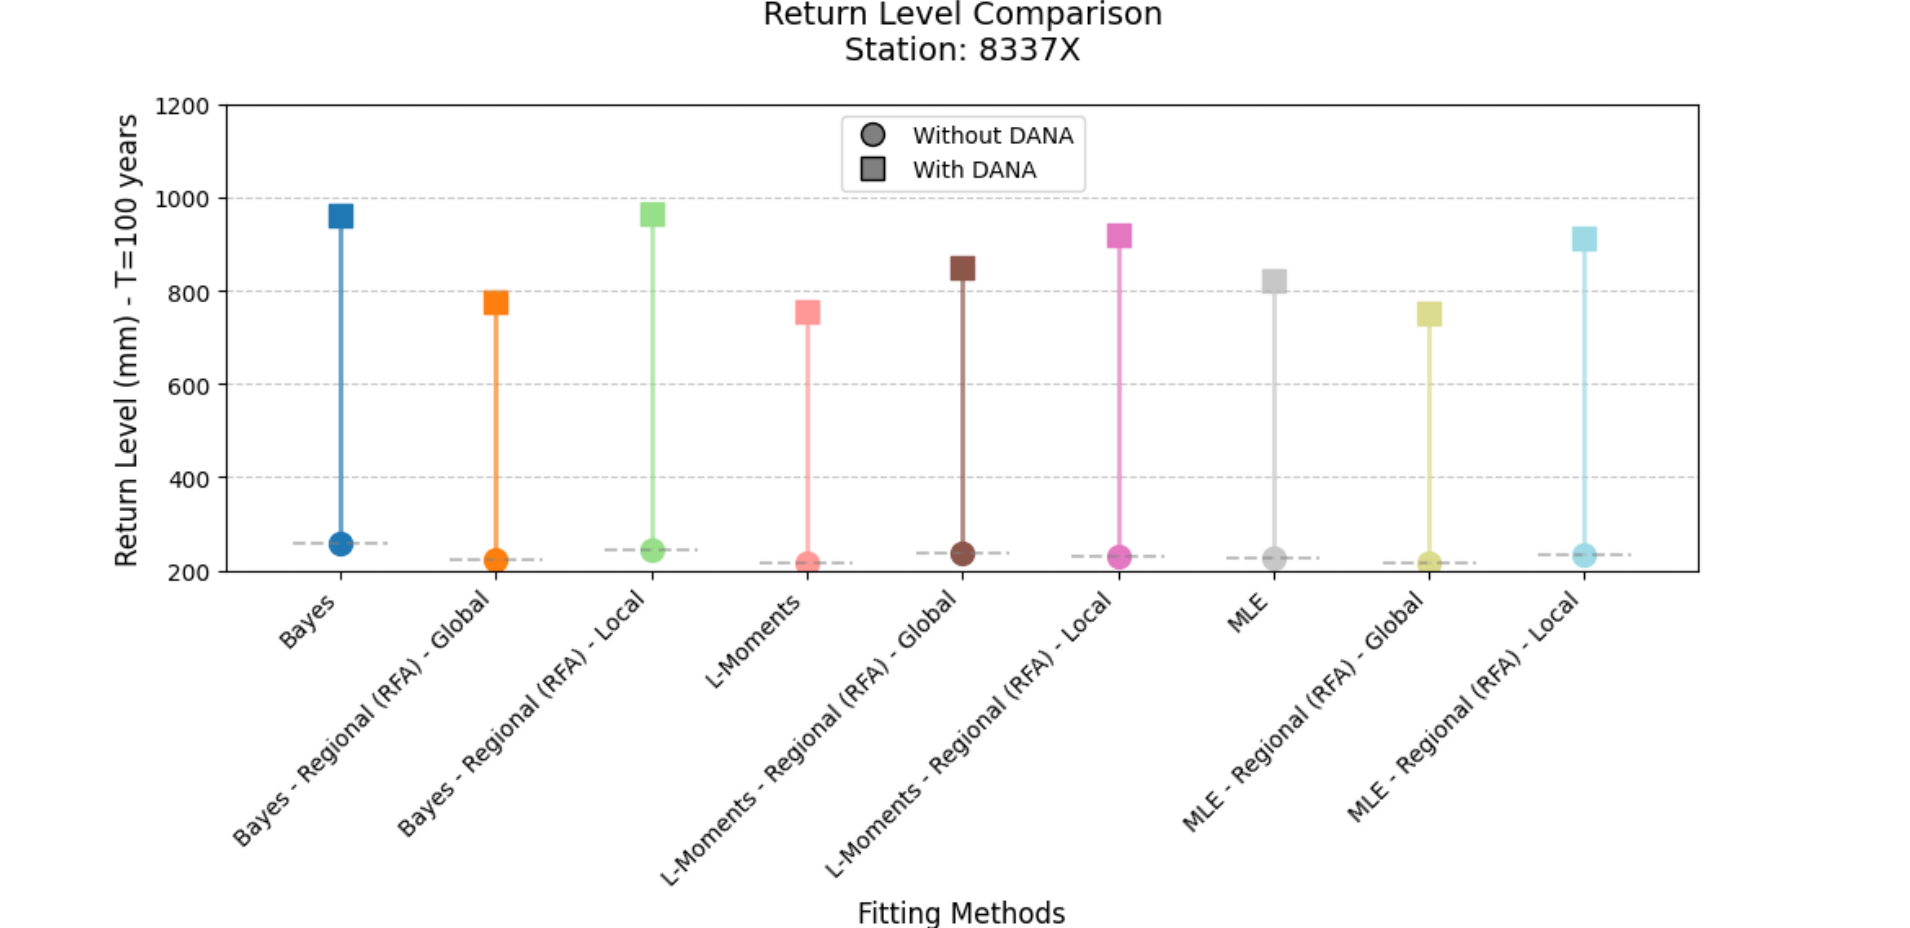
\includegraphics[width=\textwidth]{figures/fig_valencia_return_levels_8337X_clean.png}
    \caption{Turís (8337X).}
    \label{fig:valencia_rl_turis}
  \end{subfigure}
  \vspace{0.8em}
  \begin{subfigure}{0.94\textwidth}
    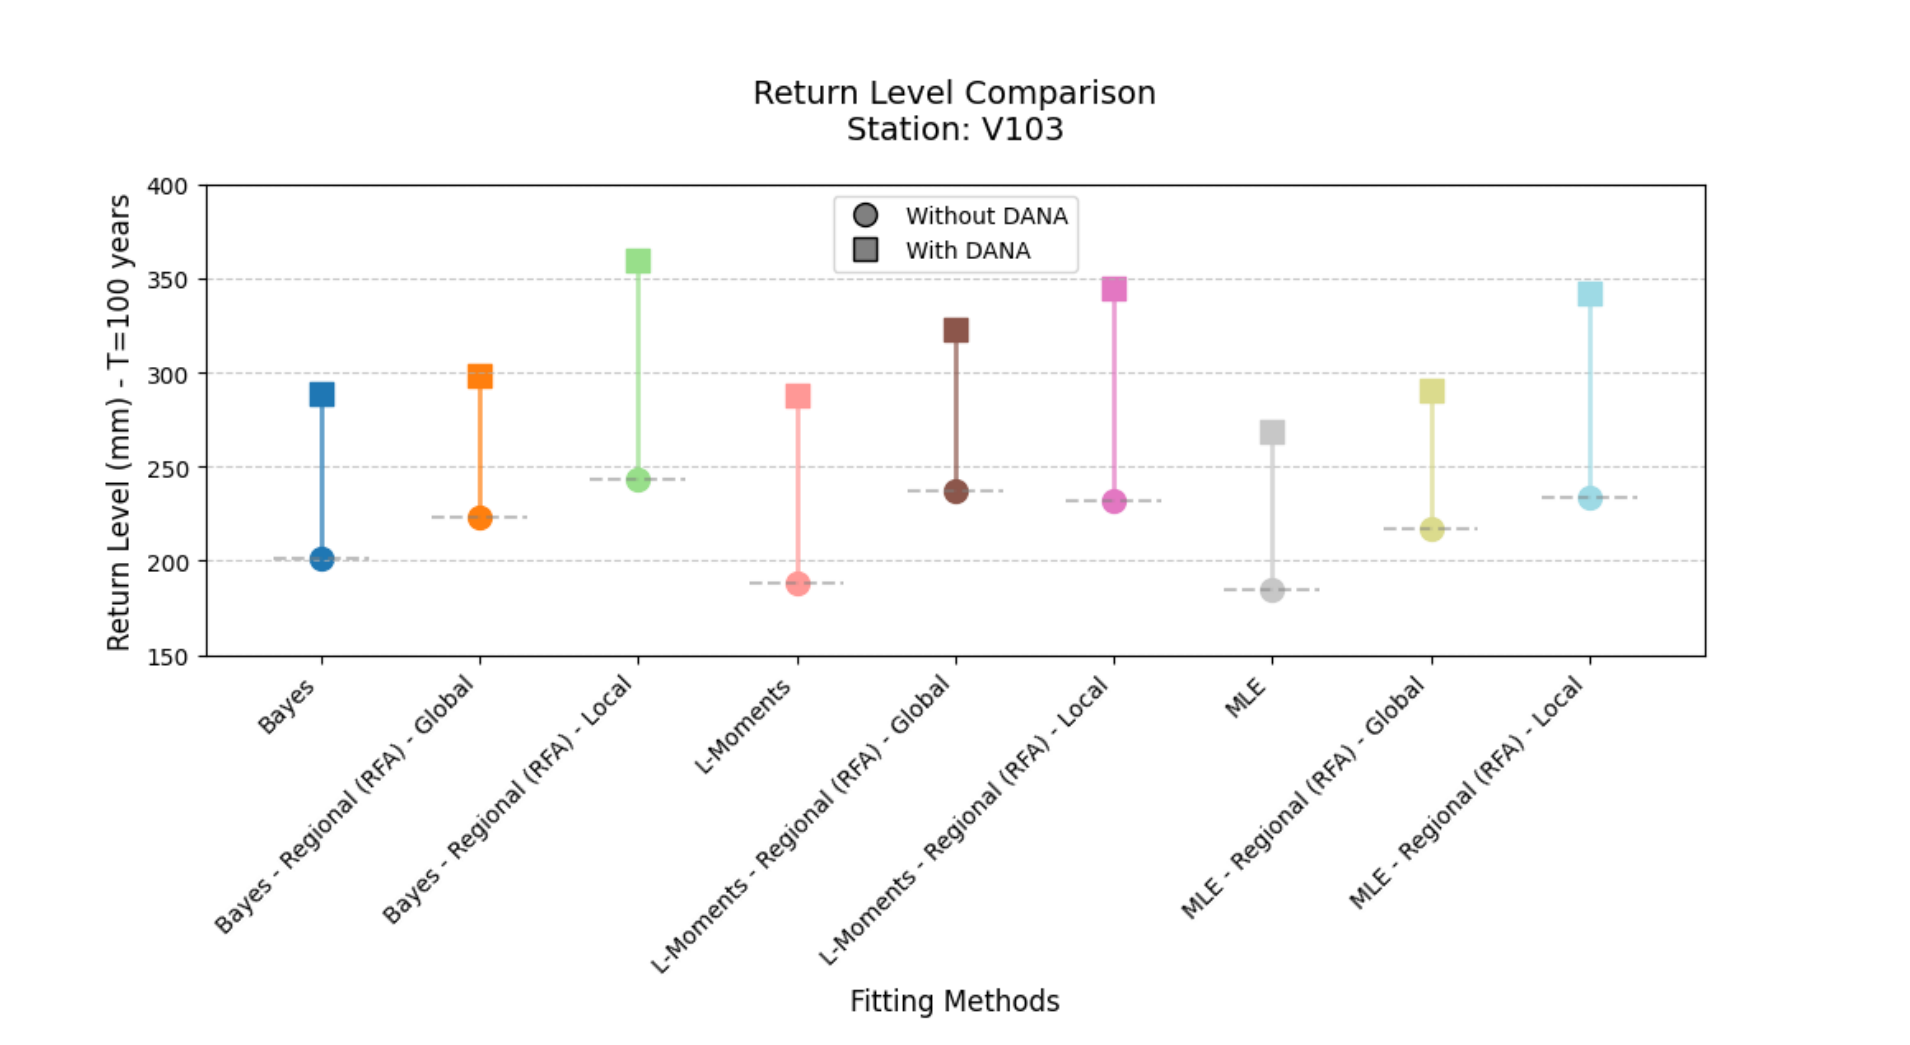
\includegraphics[width=\textwidth]{figures/fig_valencia_return_levels_V103_clean.png}
    \caption{Carlet (V103).}
    \label{fig:valencia_rl_carlet}
  \end{subfigure}
  \caption{Comparación de niveles de retorno para $T=100$ años en las estaciones de Turís y Carlet, con y sin inclusión del episodio DANA del 29 de octubre de 2024. La figura procede del análisis reproducible del caso Valencia \parencite{navas2025valenciaIA} y se incorpora como evidencia de contraste metodológico.}
  \label{fig:valencia_return_levels}
\end{figure}

\subsection{Conexión con HYDRA}

El caso Valencia valida los módulos de análisis de extremos de \path{pyhydra.climate.time_series} en un escenario de urgencia post-evento. La comparación entre MLE, L-momentos y estimación bayesiana sobre las mismas series, con y sin inclusión del evento, ilustra con datos reales por qué la disponibilidad de múltiples métodos de estimación es esencial para comunicar adecuadamente la incertidumbre. La implementación del RFA en \path{pyhydra.climate.spatial_analysis} permite reproducir el flujo completo, desde la descarga de datos de las redes AEMET, SIAR y AVAMET hasta la estimación de cuantiles regionales con intervalos credibles.

La conclusión principal del estudio \parencite{navas2025valenciaIA} es que el método bayesiano proporciona estimaciones más estables y coherentes entre escenarios que los métodos clásicos, al representar explícitamente la incertidumbre en los parámetros y en los cuantiles de retorno. Esta conclusión refuerza la decisión de incluir \texttt{fit\_gev\_mcmc} como alternativa preferente en \hydra para análisis en regiones con alta variabilidad o series cortas.

\clearpage
\section{Lago Tanganica: niveles de diseño bajo cambio climático}
\label{sec:caso_tanganika}

\subsection{Contexto y problema}

El Lago Tanganica, en la región de los Grandes Lagos de África, es una masa de agua compartida por Burundi, República Democrática del Congo, Tanzania y Zambia, con una cuenca de más de 230.000 km\textsuperscript{2}. La variabilidad creciente de sus niveles, atribuida al cambio climático, plantea riesgos directos sobre infraestructuras costeras como el puerto de Kalundu (Burundi). El diseño de la nueva infraestructura portuaria requiere definir cotas de nivel para distintos períodos de retorno bajo escenarios futuros de emisión, en un contexto donde los registros instrumentales continuos son muy limitados \parencite{navas2025tanganika}.

Este caso ilustra cómo la metodología de \hydra puede extenderse a sistemas lacustres en regiones con escasa instrumentación, combinando datos de teledetección, reanálisis climático y proyecciones CMIP6.

\subsection{Metodología aplicada}

La cadena metodológica se estructura en cinco etapas secuenciales. La primera estima los caudales mensuales de entrada al lago a partir de variables climáticas del reanálisis ERA5 \parencite{hersbach2020era5} mediante un modelo de regresión multivariante. Las variables predictoras (precipitación, temperatura máxima y mínima, radiación solar, velocidad del viento) se normalizan por celda y se someten a análisis de componentes principales para eliminar la multicolinealidad. Se comparan varios algoritmos de aprendizaje automático (regresión lineal, Elastic Net, SVR, árboles de decisión, Gradient Boosting, AdaBoost). El modelo seleccionado, AdaBoost Regressor, obtiene un coeficiente de determinación $R^2 > 0{,}85$ en validación cruzada y $R^2 = 0{,}96$ sobre el conjunto completo, con RMSE inferior al 10\% del rango observado.

La segunda etapa construye una función empírica continua caudal-nivel $N(Q)$ mediante K-means (3 clusters: caudales bajos, medios y altos) y ajuste de funciones polinómicas de segundo grado para los dos primeros grupos y una función potencial para el tercero. Esta función transforma las series de caudal simuladas en series de nivel del lago, incorporando la no linealidad de la respuesta hidrológica.

La tercera etapa incorpora la señal del cambio climático mediante downscaling estadístico de 19 modelos CMIP6 bajo los escenarios SSP2-4.5 y SSP5-8.5. Se emplea el método delta mes a mes disponible en \texttt{pyhydra.climate.bias\_correction}, que conserva la variabilidad espacial y temporal de las observaciones ERA5 mientras incorpora la anomalía climática proyectada. Los datos CMIP6 se descargan vía CDS con \texttt{pyhydra.data\_sources.climate\_change}.

La cuarta etapa genera series sintéticas de nivel mediante remuestreo bootstrap de los residuos del modelo caudal-nivel por tramo. Para cada mes de cada realización se añade a $\tilde{N}(Q_t)$ un residuo aleatorio extraído de la distribución empírica del tramo correspondiente. Este proceso se repite 1.000-2.000 veces por combinación de modelo y escenario, generando un total de aproximadamente 20.000 años simulados que cubren explícitamente la incertidumbre de la función empírica $N(Q)$.

La quinta etapa estima los niveles extremos de forma no paramétrica a partir de los percentiles empíricos de los máximos anuales del conjunto sintético. Las variaciones proyectadas $\Delta Nivel(T, t) = N_{fut}(T, t) - N_{hist}(T)$ se aplican sobre los niveles históricos obtenidos con GEV ajustada a la serie observada de altimetría satelital (Hydroweb, 1992-2023), generando proyecciones absolutas de nivel que combinan la robustez empírica del registro histórico con la señal climática proyectada.

\subsection{Resultados}

Los niveles históricos extremos estimados a partir de distribuciones teóricas (GEV, Weibull) arrojan valores de 771,55-771,76 m para un período de retorno de 100 años. El enfoque bootstrap produce niveles sistemáticamente menores para los mismos períodos de retorno (770,19 m para T100), diferencia atribuible al efecto suavizador del remuestreo sobre los valores extremos atípicos.

Las proyecciones bajo cambio climático muestran incrementos sistemáticos de los niveles máximos a lo largo del siglo XXI en ambos escenarios. El mayor incremento proyectado se alcanza en el período 2041-2060, donde los niveles máximos asociados a períodos de retorno cortos (T5-T10) aumentan más de 0,9 m respecto al histórico. Hacia el final del siglo (2081-2100), los incrementos se estabilizan por debajo de 0,6 m para los períodos de retorno largos (T100-T500), efecto atribuido a la expansión superficial del lago que amortigua los cambios de nivel a medida que el volumen adicional se distribuye sobre una mayor área. Las diferencias entre SSP2-4.5 y SSP5-8.5 son marcadas en las primeras décadas y convergen hacia el final del siglo.

\begin{figure}[htbp]
  \centering
  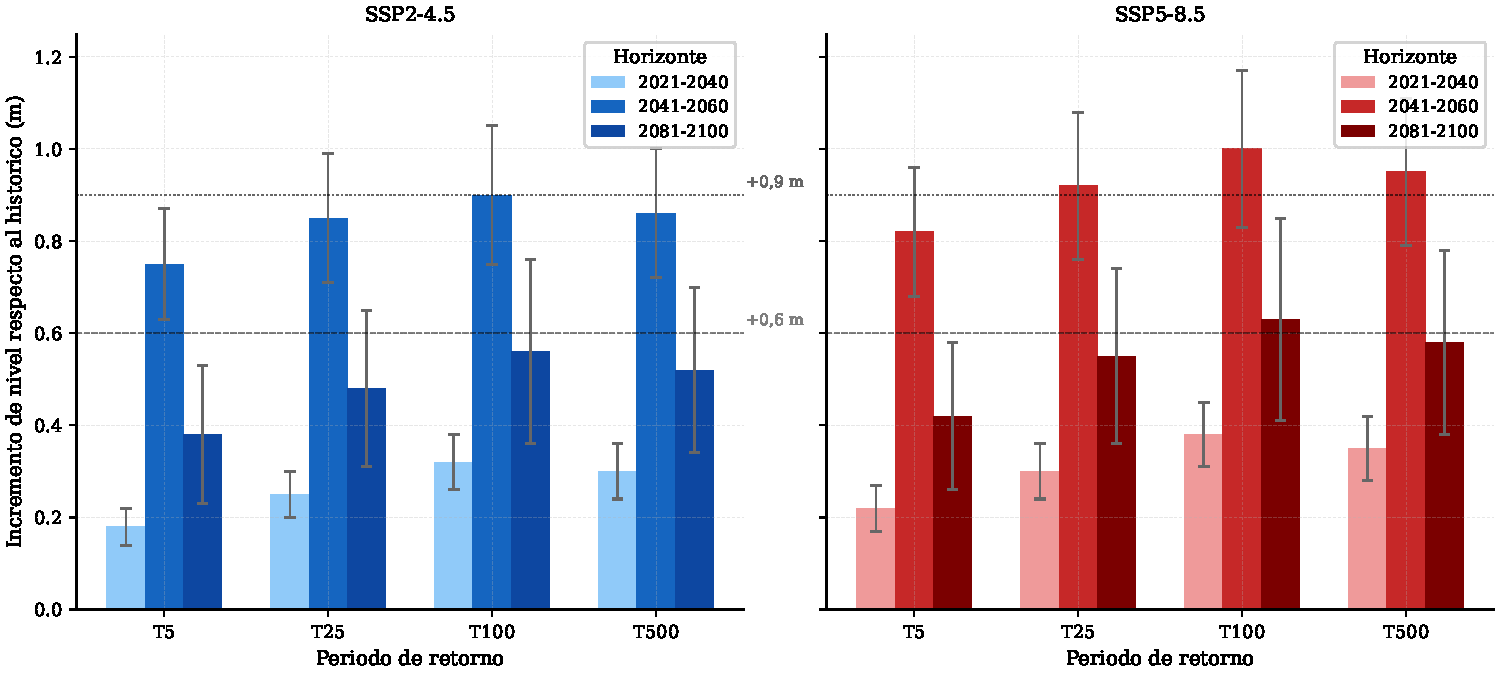
\includegraphics[width=\linewidth]{figures/fig_tanganika_proyecciones}
  \caption{Evolución del caudal mensual proyectado de entrada al Lago Tanganica (m$^3$/s), estimado con el modelo AdaBoost bajo condiciones históricas (gris) y bajo los escenarios de cambio climático SSP2-4.5 (azul) y SSP5-8.5 (rojo), con bandas de incertidumbre intermodelo. La línea vertical marca el inicio del período de proyección (2022). Ambos escenarios proyectan un incremento sostenido del caudal medio hacia finales del siglo XXI, con mayor variabilidad interanual. Figura reproducida de \parencite{navas2025tanganicaIA}.}
  \label{fig:tanganika_proyecciones}
\end{figure}

\begin{figure}[htbp]
  \centering
  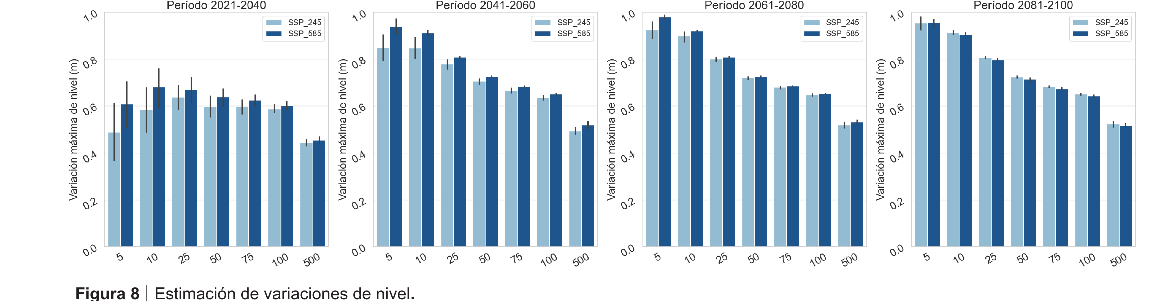
\includegraphics[width=\linewidth]{figures/fig_tanganika_variaciones_nivel}
  \caption{Variación máxima de nivel del Lago Tanganica respecto al histórico (m) para períodos de retorno de 5 a 500 años, en cuatro horizontes temporales (2021--2040, 2041--2060, 2061--2080, 2081--2100), bajo los escenarios SSP2-4.5 (azul claro) y SSP5-8.5 (azul oscuro). Las barras de error representan la incertidumbre del ensemble de 19 modelos CMIP6. El mayor incremento proyectado se alcanza en el período 2041--2060 para períodos de retorno cortos (T5--T10, $>$0,9 m); hacia finales del siglo los incrementos se estabilizan por debajo de 0,6 m para T $\geq$ 100 años. Figura reproducida de \parencite{navas2025tanganicaIA}.}
  \label{fig:tanganika_variaciones_nivel}
\end{figure}

\subsection{Conexión con HYDRA}

El caso Tanganica valida la cadena de cambio climático de \hydra en un contexto de escasa instrumentación y alta exposición: descarga de ERA5 y CMIP6, corrección de sesgo por método delta, generación sintética mediante bootstrap de residuos y análisis de extremos no paramétrico. Es la primera aplicación de la metodología a un sistema lacustre fuera de Europa, lo que demuestra la transferibilidad del enfoque a contextos con limitaciones de datos.

La combinación de regresión ML para estimar caudales a partir de variables climáticas, y de K-means para capturar la no linealidad de la respuesta del lago, es una extensión natural de los módulos de análisis estadístico de \hydra que no requiere modificar la arquitectura base del paquete.

\clearpage
\section{Vulnerabilidad de centrales hidroeléctricas andinas ante el cambio climático}
\label{sec:caso_andes}

\subsection{Contexto y problema}

La producción de energía hidroeléctrica en los países andinos ---Bolivia, Colombia, Ecuador y Perú--- depende de regímenes hidrológicos condicionados por la orografía de la cordillera, los patrones de precipitación estacional y los ciclos ENSO. La estimación de la vulnerabilidad de esta infraestructura frente al cambio climático requiere cubrir cuatro países, centenares de cuencas y varias décadas de proyecciones, con datos pluviométricos de calidad heterogénea y escasa cobertura en las zonas amazónicas \parencite{deljesus2019andean}. El caso pone a prueba la capacidad de los flujos de análisis de \hydra para gestionar datos de fuentes globales a escala regional.

\subsection{Metodología aplicada}

Los datos de precipitación proceden de las redes meteorológicas nacionales complementadas con la base de datos global NASA para cubrir las zonas de la Amazonia con escasa instrumentación. Los campos distribuidos se construyen mediante Kriging Universal con la elevación como variable de tendencia (MDT HydroSheds a 1~km de resolución). La validación cruzada produce una correlación media de Pearson $\rho = 0{,}42$, RMSE medio de 10,47 y sesgo medio del 8{,}0\% sobre el período 1981-2010. La temperatura y las variables de balance hídrico se extraen del reanálisis CFSR, con corrección del sesgo sistemático de $\approx -6\,^\circ$C respecto a las observaciones nacionales.

Las proyecciones climáticas proceden de 21 modelos GCM del proyecto CMIP5 bajo los escenarios RCP~4.5 y RCP~8.5 para los horizontes 2011-2040, 2041-2070 y 2071-2100. El modelo hidrológico VIC (Variable Infiltration Capacity), calibrado en estaciones de aforo seleccionadas por cobertura temporal, transforma los campos climáticos en series de caudal. La calibración en la estación de referencia CachEsperanz produce NSE $= 0{,}65$ y PBIAS $= 14{,}17\%$.

\subsection{Resultados}

Las proyecciones de precipitación muestran incrementos del $+15\%$ en el corto plazo hasta el $+20\%$ en el largo plazo bajo RCP~8.5 en la vertiente occidental, con decrementos del $5\%$--$15\%$ en el norte de Colombia y partes de Bolivia. Los cambios en temperatura son sistemáticamente positivos: entre $+1\,^\circ$C a corto plazo y $+3\,^\circ$C a largo plazo bajo RCP~8.5. Los cambios proyectados en caudal son no lineales respecto a los cambios de precipitación y presentan alta variabilidad estacional: en Perú y Ecuador bajo RCP~8.5 en el período 2071-2100, los caudales de los meses más húmedos aumentan más de un 40\% respecto al histórico, mientras que en Bolivia la respuesta puede ser moderada o incluso negativa en determinados meses. Las diferencias entre modelos GCM son el principal factor de incertidumbre en todos los países.

\begin{figure}[htbp]
  \centering
  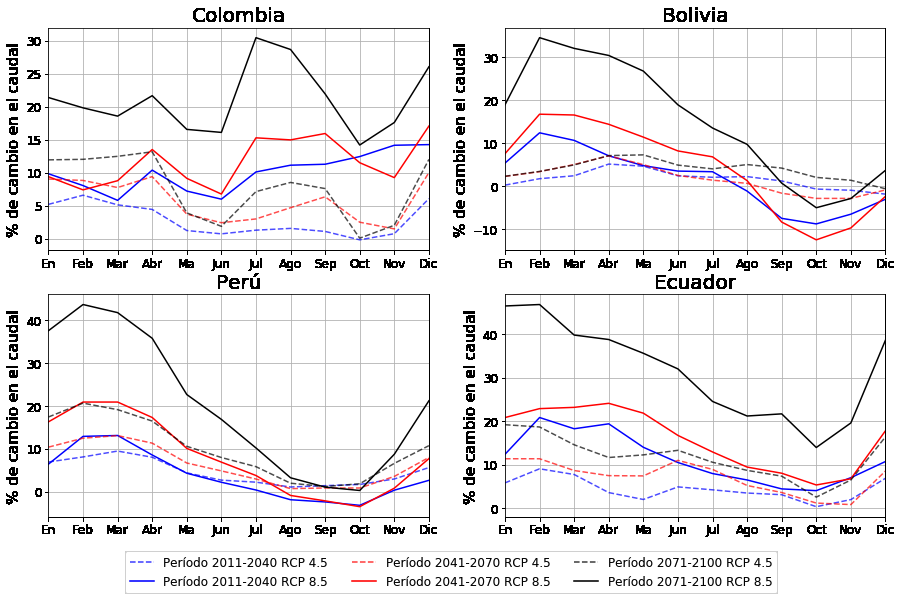
\includegraphics[width=\textwidth]{figures/fig_andes_caudales_cc.png}
  \caption{Influencia proyectada del cambio climático en el caudal mensual de Colombia, Bolivia, Perú y Ecuador para los escenarios RCP~4.5 y RCP~8.5 y tres horizontes temporales. Los cambios presentan una marcada variabilidad estacional y alcanzan valores superiores al $+40\%$ en Perú y Ecuador. Fuente: comunicación presentada en las VI Jornadas de Ingeniería del Agua \parencite{deljesus2019andean}.}
  \label{fig:andes_caudales_cc}
\end{figure}

\subsection{Conexión con HYDRA}

Este caso desarrolla tres capacidades que quedaron formalizadas en \hydra: la descarga automatizada de reanálisis y proyecciones globales (\path{pyhydra.data_sources.climate_change}), la interpolación de campos distribuidos con Kriging Universal y covariables topográficas (\path{pyhydra.climate.spatial_analysis}), y la corrección de sesgo mediante mapeo de cuantiles (\path{pyhydra.climate.bias_correction}). La escala regional ---cuatro países, más de 200 subcuencas, 21 modelos GCM--- anticipa la arquitectura de procesamiento masivo que \hydra formaliza con APIs uniformes por fuente de datos y módulo de análisis.

\clearpage
\section{Impacto de las decisiones metodológicas en el riesgo de inundación bajo cambio climático}
\label{sec:caso_iahr2022}

\subsection{Contexto y problema}

La práctica convencional asigna directamente el período de retorno de la precipitación al caudal pico obtenido a partir del hietograma de diseño correspondiente. Esta transferencia es conceptualmente incorrecta en cuencas no lineales, donde la distribución de probabilidad del impacto hidráulico no coincide con la del forzamiento meteorológico. El trabajo de \textcite{deljesus2022iahr}, presentado en el 39th IAHR World Congress (Granada, 2022), cuantifica sistemáticamente la diferencia entre esta aproximación estándar y la metodología estocástica de \hydra en una cuenca del norte de España con régimen hidrológico atlántico, bajo distintos escenarios y horizontes de cambio climático.

\subsection{Metodología aplicada}

El estudio emplea 15 modelos del conjunto EURO-CORDEX bajo los escenarios RCP~4.5 y RCP~8.5, con corrección de sesgo mediante mapeo de cuantiles empírico sobre el período histórico de referencia \parencite{teutschbein2012biascorrection}. Los eventos de crecida se caracterizan por caudal pico, duración y forma del hidrograma (clasificada mediante k-means), y la dependencia multivariante se modela con cópulas gaussianas. A partir de la distribución ajustada se generan 10.000 años de eventos sintéticos, de los que se seleccionan 200 casos representativos mediante el algoritmo de máxima disimilitud para su simulación hidráulica completa con Iber en régimen no permanente. Los calados del resto de eventos se reconstruyen con el emulador k-NN. El análisis de extremos se aplica directamente sobre la variable hidráulica (calado) y no sobre la precipitación forzante.

\subsection{Resultados}

La diferencia entre la metodología estocástica y la estándar es sistemática y significativa en todos los períodos de retorno, escenarios y horizontes. La \cref{tab:iahr2022_caudales} recoge los caudales de diseño para los cuatro períodos de retorno y los seis escenarios-horizonte. Los caudales de la metodología estocástica son entre un 30\% y un 37\% superiores en todos los casos.

\begin{table}[htbp]
  \centering
  \caption{Caudales de diseño (m\textsuperscript{3}/s) estimados con la metodología estocástica de \hydra y la metodología estándar basada en curvas IDF, para cuatro períodos de retorno, dos escenarios de cambio climático y tres horizontes temporales. La diferencia entre enfoques es del 30--37\% en todos los casos. Fuente: \parencite{deljesus2022iahr}.}
  \label{tab:iahr2022_caudales}
  \resizebox{\textwidth}{!}{%
  \begin{tabular}{llrrrr}
    \toprule
    Escenario & Metodología & $T$ (años) & 2011--2040 & 2041--2070 & 2071--2100 \\
    \midrule
    \multirow{8}{*}{RCP~4.5}
      & \multirow{4}{*}{Estocástica}
        & 50  & 249,9 & 257,1 & 265,7 \\
      & & 100 & 278,5 & 286,6 & 296,8 \\
      & & 200 & 317,3 & 326,8 & 339,2 \\
      & & 500 & 362,3 & 373,5 & 388,4 \\
    \cmidrule{2-6}
      & \multirow{4}{*}{Estándar (IDF)}
        & 50  & 187,4 & 192,8 & 199,3 \\
      & & 100 & 208,8 & 214,9 & 222,6 \\
      & & 200 & 238,0 & 245,1 & 254,4 \\
      & & 500 & 271,7 & 280,1 & 291,3 \\
    \midrule
    \multirow{8}{*}{RCP~8.5}
      & \multirow{4}{*}{Estocástica}
        & 50  & 258,8 & 262,5 & 271,2 \\
      & & 100 & 288,7 & 293,0 & 303,1 \\
      & & 200 & 329,4 & 334,7 & 346,7 \\
      & & 500 & 376,7 & 383,0 & 397,4 \\
    \cmidrule{2-6}
      & \multirow{4}{*}{Estándar (IDF)}
        & 50  & 194,1 & 196,9 & 203,4 \\
      & & 100 & 216,5 & 219,8 & 227,3 \\
      & & 200 & 247,1 & 251,0 & 260,0 \\
      & & 500 & 282,5 & 287,3 & 298,1 \\
    \bottomrule
  \end{tabular}}
\end{table}

Los mapas de inundación resultantes no son proporcionales a la diferencia en caudales, lo que evidencia la no linealidad del sistema y descarta cualquier factor de corrección simple aplicable a los resultados de la metodología estándar. La diferencia entre enfoques es mayor que la incertidumbre intermodelo de los escenarios climáticos para todos los períodos de retorno considerados.

\begin{figure}[htbp]
  \centering
  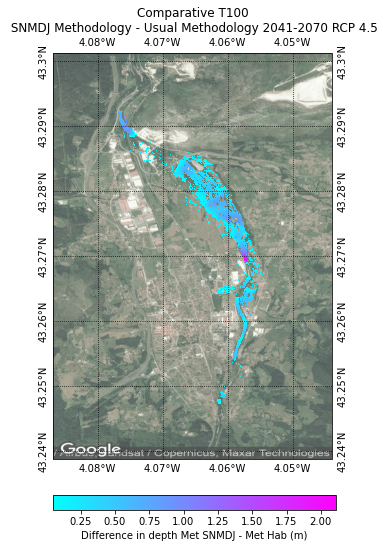
\includegraphics[height=0.58\textheight]{figures/fig_iahr2022_comparativa.png}
  \caption{Diferencia espacial de calado para $T = 100$ años entre la metodología estocástica y la metodología habitual bajo RCP~4.5 en el horizonte 2041--2070. La distribución espacial confirma que la discrepancia entre enfoques no puede representarse mediante un factor uniforme sobre el caudal. Fuente: presentación del 39th IAHR World Congress \parencite{deljesus2022iahr}.}
  \label{fig:iahr2022_mapas}
\end{figure}

\subsection{Conexión con HYDRA}

Este trabajo proporciona la primera validación cuantitativa del error sistemático introducido por la metodología estándar en estudios de inundación bajo cambio climático. Los módulos validados son los mismos que los del Besaya y Calle 30: corrección de sesgo (\texttt{pyhydra.climate.bias\_correction}), generación estocástica con cópulas (\texttt{pyhydra.climate.spatial\_analysis}), selección por máxima disimilitud (\texttt{pyhydra.climate.hybrid\_downscaling}) y reconstrucción k-NN del dominio hidráulico. La conclusión de que la elección de metodología es una fuente de incertidumbre de primer orden sustenta la hipótesis central de la tesis: la metodología estocástica basada en impactos no es un refinamiento opcional, sino una condición para obtener estimaciones de riesgo no sesgadas.

\clearpage
\section{SIMPCCe: aportaciones a embalses bajo cambio climático}
\label{sec:caso_simpce}

\subsection{Contexto y problema}

El cambio climático puede reducir sistemáticamente las aportaciones disponibles en épocas de estiaje en las cuencas españolas, comprometiendo el suministro en sistemas regulados. Cuantificar este impacto requiere combinar reanálisis histórico, proyecciones de modelos climáticos, corrección de sesgo y modelización hidrológica sobre cualquier punto de la red hídrica nacional. SIMPCCe responde a esa necesidad mediante una cadena Python para evaluar aportaciones a embalses bajo escenarios climáticos, desarrollada en el marco de la guía metodológica de Fundación Canal para la estimación de aportaciones mínimas a embalses en el contexto de cambio climático \parencite{fundacioncanal2022guiaembalses}. La herramienta fue presentada en JIA 2023 \parencite{navas2023simpce} y en el congreso europeo de IAHR de 2024 \parencite{navas2024iahrsimpcce}, y publicada posteriormente como artículo en \textit{Ingeniería del Agua} \parencite{navas2025simpce}, una de las publicaciones que integran el compendio de resultados de esta tesis. La aplicación integra módulos climáticos de \pyhydra en un flujo orientado a gestores del recurso hídrico; además, el Observatorio del Agua de la Fundación Botín reconoció el trabajo con el Premio al Talento Joven ``M.R. Llamas''.

\subsection{Metodología aplicada}

SIMPCCe consta de cinco módulos que se corresponden directamente con capacidades de \hydra. El primero descarga automáticamente datos de precipitación y temperatura del conjunto SPAIN02~v5 \parencite{herrera2016spain02} y aportaciones del modelo SIMPA-CEDEX para el período 1950-2015, junto con 10 modelos del proyecto CORDEX-AEMET bajo los escenarios RCP~4.5 y RCP~8.5 para tres horizontes temporales. El segundo delimita la cuenca aportante al punto de interés a partir de un MDT de 200~m y extrae la malla de puntos climáticos distribuidos. El tercero entrena una red neuronal artificial (ANN) sobre las componentes principales de la precipitación y temperatura distribuidas (PCA al 95\% de la varianza, división 80/20 entrenamiento/validación) para predecir las aportaciones mensuales. El cuarto aplica la corrección de sesgo SDM \parencite{switanek2017sdm} a cada combinación modelo-escenario-horizonte, generando 60 series corregidas por variable (10 modelos $\times$ 2 escenarios $\times$ 3 períodos). El quinto simula 20 series futuras de aportaciones con la ANN entrenada y sintetiza los resultados en informes automáticos con estadísticas anuales, SPI e índices de fiabilidad para la toma de decisiones.

\subsection{Resultados}

Las conclusiones del análisis a escala nacional con 10 modelos CORDEX confirman que el cambio climático reduce sistemáticamente las aportaciones medias anuales en la mayoría de las cuencas españolas, que las aportaciones mínimas en épocas de estiaje disminuyen incluso en cuencas donde la precipitación media no registra cambios estadísticamente significativos, y que la sequía hidrológica tiende a aumentar en severidad y duración bajo ambos escenarios. La envolvente intermodelo permite cuantificar la incertidumbre y orientar decisiones de planificación con distintos niveles de cautela.

\begin{figure}[htbp]
  \centering
  \begin{subfigure}[t]{0.47\textwidth}
    \centering
    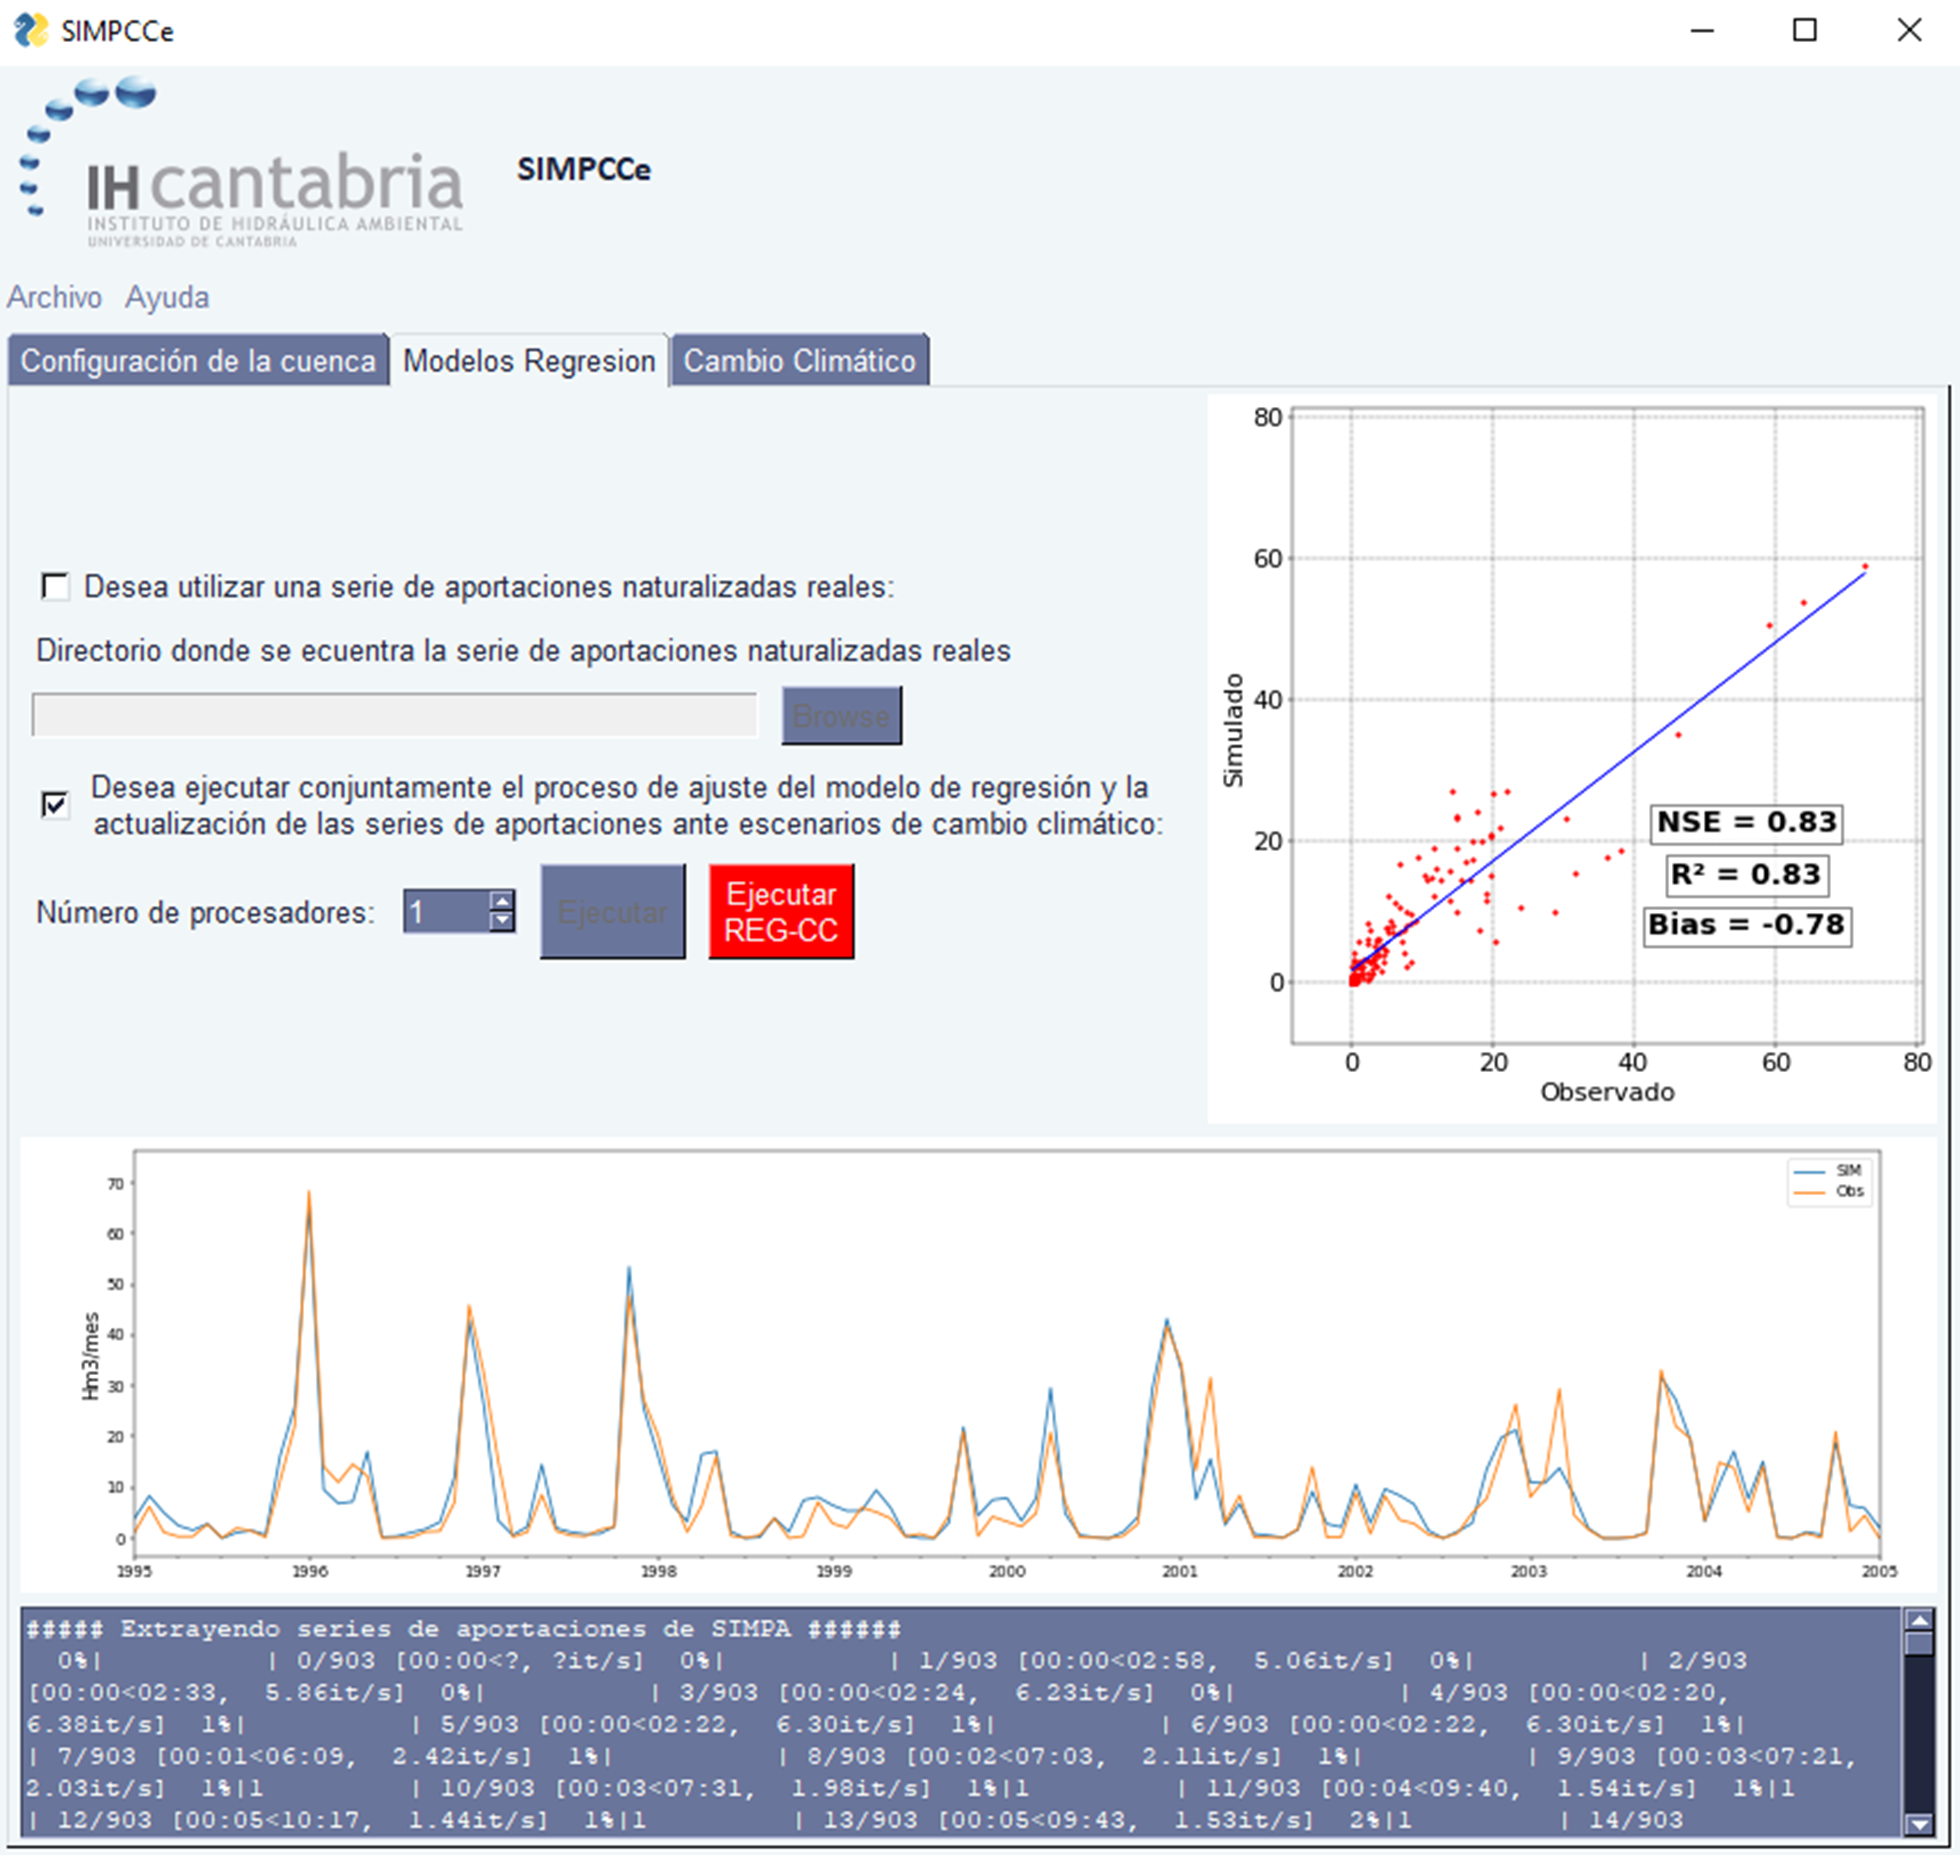
\includegraphics[width=\textwidth]{figures/fig_simpcce_interfaz.png}
    \caption{Interfaz de entrenamiento y validación.}
  \end{subfigure}
  \hfill
  \begin{subfigure}[t]{0.50\textwidth}
    \centering
    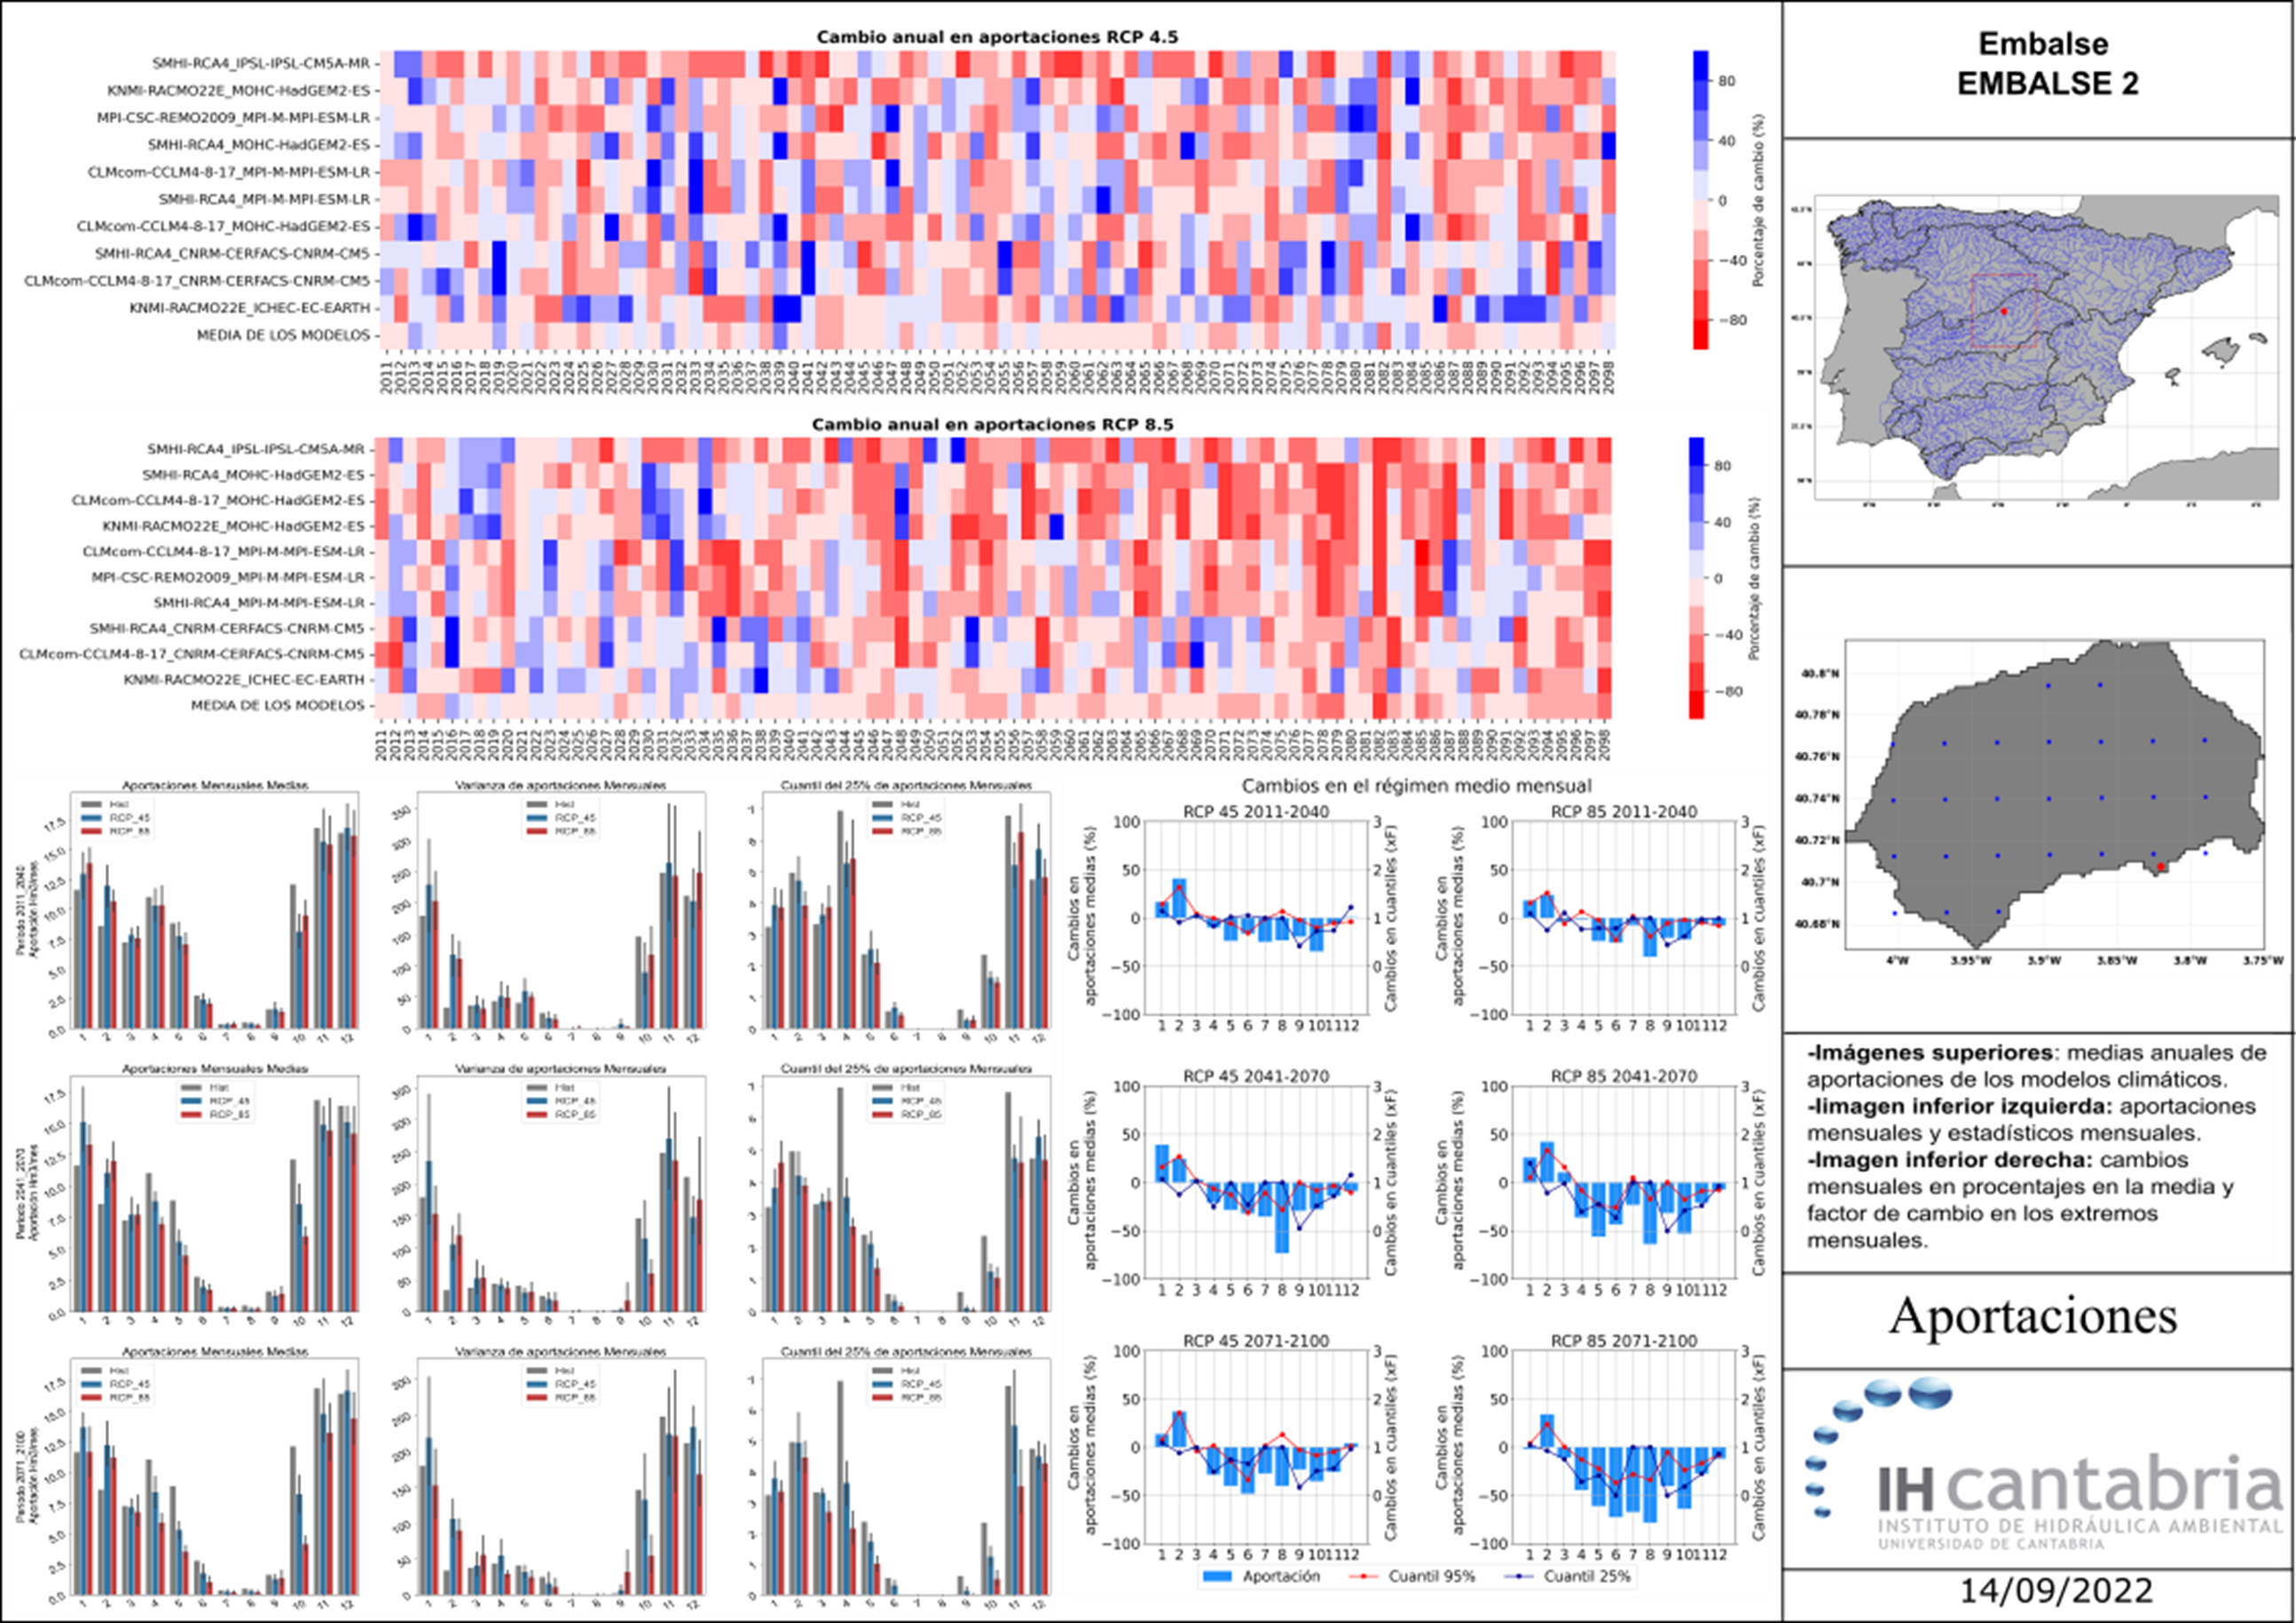
\includegraphics[width=\textwidth]{figures/fig_simpcce_resultados.png}
    \caption{Ficha automática de cambio en aportaciones.}
  \end{subfigure}
  \caption{Productos operativos de SIMPCCe. La interfaz permite ejecutar la cadena de cálculo y validar la red neuronal; las fichas sintetizan los cambios anuales y mensuales bajo RCP~4.5 y RCP~8.5, junto con la incertidumbre intermodelo. Fuentes: presentaciones JIA 2023 e IAHR Europe 2024 \parencite{navas2023simpce,navas2024iahrsimpcce}.}
  \label{fig:simpce_output}
\end{figure}

\subsection{Conexión con HYDRA}

SIMPCCe es el caso de uso más completo del bloque de cambio climático de \hydra: los módulos \texttt{pyhydra.data\_sources.climate\_change}, \texttt{pyhydra.climate.bias\_correction} y \texttt{pyhydra.climate.time\_series} operan integrados como una cadena de cálculo. La conexión de la herramienta con la guía metodológica para la estimación de aportaciones mínimas a embalses promovida por Fundación Canal \parencite{fundacioncanal2022guiaembalses} ilustra la dimensión industrial de la investigación y su transferencia a problemas reales de planificación de recursos hídricos.

\clearpage
\section{Atlas de Riesgo Climático de la República de Panamá}
\label{sec:caso_panama}

\subsection{Contexto y problema}

El Atlas Interactivo de Riesgo Climático de Panamá \parencite{ihcantabria2023panama} es la aplicación de mayor escala geográfica realizada con las herramientas de \hydra. El proyecto, encargado por la Dirección de Cambio Climático del Ministerio de Ambiente y financiado por el Banco Interamericano de Desarrollo, abarca las 52 cuencas hidrológicas del país ---18 en la vertiente caribe y 34 en la del Pacífico--- con superficies individuales de hasta 13.400~km\textsuperscript{2}. El proyecto cuantifica de forma integrada los riesgos climáticos para los horizontes 2030, 2050 y 2070 bajo los escenarios SSP2-4.5 y SSP5-8.5, incluyendo inundación fluvial en las 52 cuencas, inundación costera en 1.464 puntos de ambas costas, y viento extremo sobre el área metropolitana de Ciudad de Panamá.

\subsection{Metodología aplicada}

La cadena metodológica moviliza los tres bloques funcionales de \hydra en una ejecución a escala nacional. El bloque de datos descarga ERA-5 \parencite{hersbach2020era5}, precipitación TRMM/TMPA \parencite{huffman2007trmm} y proyecciones de 23 modelos CMIP6 \parencite{eyring2016cmip6} bajo SSP2-4.5 y SSP5-8.5 para el período 1950-2100. NEOPRENE \parencite{diezsierra2023neoprene}, mediante sus generadores NSRP/STNSRP, rellena los huecos en 73 estaciones meteorológicas nacionales para el período 1950-2022. Los campos de precipitación se interpolan a malla de 1~km mediante Kriging Universal con elevación y precipitación media TRMM como covariables.

La corrección de sesgo se ejecuta en 414 combinaciones (23 modelos $\times$ 2 escenarios $\times$ 6 variables $\times$ 3 períodos) mediante QDM para precipitación \parencite{cannon2015sdm} y SDM para temperatura \parencite{switanek2017sdm}. El modelo hidrológico LEM ---calibrado con Nash-Sutcliffe NS $= 0{,}87$ en las estaciones de referencia--- simula los caudales en 200-300 subcuencas; los caudales máximos para períodos de retorno de 10, 50 y 100 años se calculan con ajuste GEV mediante \texttt{pyhydra.climate.time\_series.extremes}. Las manchas de inundación fluvial se generan con el modelo SFINCS para el conjunto nacional y con modelos hidráulicos 2D de alta resolución para el área metropolitana.

\subsection{Resultados}

El atlas publica seis familias de capas de riesgo en un visor web interactivo del Ministerio de Ambiente. Las capas de inundación fluvial cubren las 52 cuencas para tres períodos de retorno ($T = 10, 50, 100$ años) y tres horizontes temporales bajo dos escenarios SSP. Las capas de inundación costera comprenden 52 escenarios de nivel de agua total en los 1.464 puntos costeros analizados a lo largo de ambas costas. Las proyecciones de índices climáticos extremos (SPI, SPEI, RX1, RX5 y otros) se calculan para los tres horizontes temporales. La dimensión operativa del proyecto ---23 modelos GCM, 414 correcciones de sesgo, 200-300 subcuencas, miles de simulaciones SFINCS--- ilustra la capacidad de \hydra para ejecutar flujos de análisis masivos sin modificar la arquitectura base del sistema.

\begin{figure}[htbp]
  \centering
  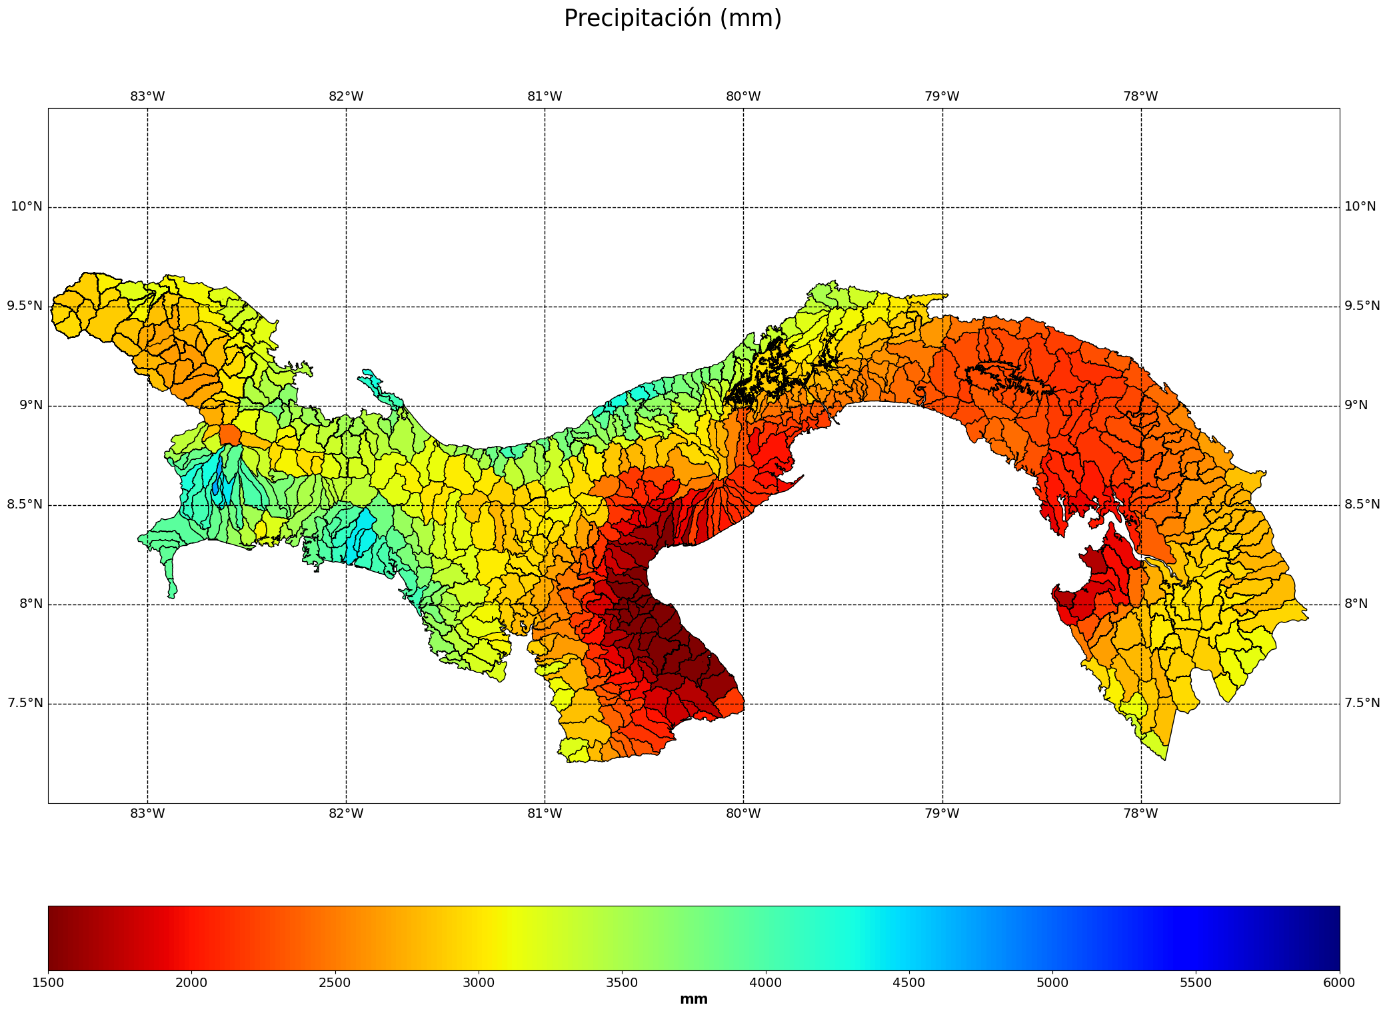
\includegraphics[width=\textwidth]{figures/fig_panama_precipitacion.png}
  \caption{Precipitación media distribuida por subcuencas para la República de Panamá, obtenida mediante el flujo nacional de descarga, control de calidad e interpolación espacial que alimenta los modelos hidrológicos y las ejecuciones masivas de SFINCS. Fuente: memoria técnica del Atlas de Riesgo Climático de Panamá \parencite{ihcantabria2023panama}.}
  \label{fig:panama_atlas}
\end{figure}

\subsection{Conexión con HYDRA}

El Atlas de Panamá es la aplicación más amplia de \hydra en un contexto de encargo industrial a escala nacional. El proyecto fue el primer banco de pruebas a gran escala del bloque de datos (\texttt{pyhydra.data\_sources}) para la descarga y procesamiento de ERA-5, CMIP6 y datos TRMM; del módulo de corrección de sesgo (\texttt{pyhydra.climate.bias\_correction}) para el procesamiento masivo de 23 modelos y 6 variables; y de la interfaz SFINCS (\texttt{pyhydra.modeling.hydraulic.sfincs}) para la generación sistemática de manchas de inundación a escala de país. Los patrones de automatización y reutilización de configuración validados en este proyecto se trasladaron directamente a la arquitectura final de \hydra.

\clearpage
\section{Síntesis de la validación}
\label{sec:sintesis_validacion}

\subsection{Cobertura de módulos}

Los nueve casos de estudio cubren conjuntamente todos los módulos de \hydra a distintas escalas, regímenes hidrológicos y contextos institucionales. La \cref{tab:validacion_modulos} resume la correspondencia entre casos y módulos validados.

\begin{table}[htbp]
  \centering
  \caption{Cobertura de módulos de \pyhydra por caso de estudio.}
  \label{tab:validacion_modulos}
  \small
  \begin{tabular}{>{\raggedright\arraybackslash}p{0.24\textwidth}>{\raggedright\arraybackslash}p{0.64\textwidth}}
    \toprule
    Caso & Módulos validados \\
    \midrule
    Mallorca & SIAR, PERSIANN/TRMM como diagnóstico, kriging espacial, cópulas gaussianas, MaxDiss, k-NN, downscaling híbrido desde lluvia; simulación hidráulica con Iber (herramienta externa, sin adaptador en \pyhydra) \\
    Besaya & Extremos de caudal, cópulas gaussianas, HEC-RAS/SFINCS en desarrollos posteriores \parencite{navas2018besaya}; Iber como motor hidráulico externo en la aplicación inicial de 2018 \\
    Calle 30 & ERA5, extremos precipitación, cópulas multivariantes, HEC-HMS, HEC-RAS 1D, downscaling híbrido, períodos de retorno por pixel \\
    Valencia 2024 & AEMET/SIAR/AVAMET, GEV (MLE, L-momentos, MCMC con PyMC), RFA, cuantificación de incertidumbre \\
    Tanganica & ERA5, CMIP6, corrección de sesgo delta, regresión ML (AdaBoost), K-means, bootstrap sintético, extremos no paramétricos \\
    Andes (Bolivia, Colombia, Ecuador, Perú) & Kriging Universal con MDT global, CMIP5, corrección de sesgo, modelo VIC \\
    Cuenca atlántica -- CC (IAHR 2022) & EURO-CORDEX, corrección de sesgo, cópulas gaussianas, MaxDiss, k-NN, comparación metodologías; simulación hidráulica con Iber (herramienta externa) \\
    SIMPCCe & SPAIN02, CORDEX-AEMET, corrección de sesgo SDM, ANN, análisis de sequía, informes automáticos \\
    Atlas Panamá & ERA5, TRMM, CMIP6, NEOPRENE (NSRP/STNSRP), kriging 1~km, 414 correcciones SDM/QDM, GEV, SFINCS, inundación costera \\
    \bottomrule
  \end{tabular}
\end{table}

\subsection{Escala computacional gestionada}

Un indicador directo del beneficio industrial de la automatización es la escala de cálculo que cada caso gestionó sin intervención manual entre etapas. La \cref{tab:escala_computacional} recoge las magnitudes documentadas en los casos; ninguna de estas campañas habría sido operativamente viable con flujos manuales de configuración, ejecución y postprocesado caso a caso. A ellas se añade la reducción del 94\% del coste de cálculo de períodos de retorno conjuntos lograda por el emulador GPR en la línea de extensión multivariante \parencite{urrea2026vine}.

\begin{table}[htbp]
  \centering
  \caption{Indicadores de escala computacional gestionada automáticamente en los casos de estudio.}
  \label{tab:escala_computacional}
  \small
  \begin{tabular}{>{\raggedright\arraybackslash}p{0.24\textwidth}>{\raggedright\arraybackslash}p{0.64\textwidth}}
    \toprule
    Caso & Escala gestionada por la cadena automatizada \\
    \midrule
    Besaya (rugosidad) & Ensemble emparejado de 995 realizaciones de Manning ejecutado en dos motores hidráulicos 2D (1\,990 simulaciones), con carga, georreferenciación y análisis conjunto de todas las salidas \\
    Calle 30 & Miles de eventos sintéticos multisitio; subconjunto representativo simulado en HEC-HMS y HEC-RAS 1D y reconstrucción k-NN del resto sobre la red de túneles \\
    Mallorca & Miles de eventos sintéticos de precipitación; reconstrucción k-NN (6 vecinos) de calados y velocidades del conjunto no simulado \\
    Atlas de Panamá & 414 correcciones de sesgo SDM/QDM, interpolación climática nacional a 1~km, 200--300 subcuencas y ejecución sistemática de SFINCS a escala de país \\
    SIMPCCe & 60 series corregidas por variable (10 modelos $\times$ 2 escenarios $\times$ 3 horizontes) y 20 realizaciones futuras por punto de la red hídrica nacional \\
    Tanganica & 19 modelos CMIP6 bajo dos escenarios SSP con downscaling estadístico y remuestreo bootstrap \\
    \bottomrule
  \end{tabular}
\end{table}

\subsection{Transferencia y reproducibilidad}

La existencia de publicaciones para cada caso proporciona referencias externas independientes. Los 26 notebooks generales de ejemplo permiten repetir funcionalidades de \hydra con datos abiertos, sintéticos controlados o modelos oficiales de referencia, mientras que las 23 entradas de casos piloto del catálogo web documentan flujos territoriales completos. El material interno utilizado para preparar artículos, incluido el análisis de sensibilidad de Manning, se mantiene separado del catálogo general y se utiliza en este capítulo únicamente como fuente de resultados científicos del caso correspondiente.

\subsection{Limitaciones observadas}

A lo largo de los casos se han identificado tres categorías de limitaciones. Las limitaciones de datos afectan a la longitud y homogeneidad de las series disponibles. Las limitaciones computacionales derivan de la dependencia de modelos externos que requieren instalaciones específicas o tiempos de cálculo prolongados. Las limitaciones metodológicas están asociadas a la hipótesis de estacionariedad de los generadores estocásticos. Ninguna invalida la arquitectura de \hydra, pero todas se documentan en los notebooks correspondientes para que el usuario pueda evaluar su alcance antes de aplicar la herramienta a un nuevo caso.

La validación realizada no debe entenderse como una validación universal de todos los módulos en todos los contextos posibles, sino como una validación operativa de la arquitectura mediante casos que ejercitan combinaciones representativas de módulos, datos y motores externos. Los nueve casos no son experimentos homogéneos comparables entre sí, sino instancias complementarias cuya diversidad geográfica, de escala y de fenómeno es precisamente la que garantiza la generalidad funcional de \hydra.

\chapter{Conclusiones y trabajo futuro}
\label{ch:conclusiones}

La contribución doctoral original de esta tesis no es la formulación matemática de nuevos modelos hidrológicos, hidráulicos o estadísticos, sino la concepción, implementación, validación y documentación de \pyhydra como núcleo metodológico reutilizable, y de \hydra como plataforma de integración industrial. Esta arquitectura reproducible permite operacionalizar de forma integrada metodologías probabilísticas avanzadas en problemas reales de ingeniería del riesgo de inundación. La novedad reside en la integración funcional y en la transferibilidad demostrada, no en reatribuir como propios métodos estadísticos o modelos físicos preexistentes.

\section{Sobre la metodología estocástica de inundación}

La tesis ha demostrado que la generación estocástica de eventos y el análisis probabilístico de impactos hidráulicos constituyen una alternativa viable al uso exclusivo de eventos de diseño deterministas. La aplicación fundacional al Besaya \parencite{navas2018besaya} estableció el principio de estimar la frecuencia sobre calados y extensiones simuladas con Iber. Mallorca \parencite{navas2019mallorca} introdujo la primera formulación de downscaling híbrido desde lluvia, apoyada en diagnóstico PERSIANN/TRMM, reconstrucción pluviométrica por kriging, selección MaxDiss y reconstrucción k-NN. Calle 30 \parencite{navas2024calle30} consolidó posteriormente la cadena urbana con precipitación multisitio, HEC-HMS, HEC-RAS 1D y reconstrucción masiva de impactos, permitiendo obtener distribuciones de calado sin simular exhaustivamente todos los escenarios posibles.

La distinción entre el período de retorno del forzamiento meteorológico y el período de retorno del impacto hidráulico es una de las conclusiones metodológicas más relevantes. En sistemas fluviales con regulación, atenuación o efectos de confluencia, estos dos valores pueden diferir de forma significativa, lo que invalida el enfoque convencional que traslada directamente el período de retorno de la precipitación al calado de inundación. \hydra permite cuantificar esta discrepancia de forma sistemática.

El bloque de generación estocástica integra dos familias complementarias: NEOPRENE como librería que contiene los generadores NSRP puntual y STNSRP multisitio para precipitación basada en modelos de Neyman-Scott \parencite{rodriguezituribe1987,rodriguezituribe1988,diezsierra2023neoprene}, y CoSMoS como librería para generación general de series hidrológicas con dependencia temporal y marginales controladas \parencite{papalexiou2018storm}. Estas herramientas amplían el alcance de \pyhydra respecto a los primeros trabajos de inundación, en los que la generación estocástica se basaba en eventos y cópulas, no en NEOPRENE.

\section{Sobre el cambio climático y la corrección de sesgo}

La integración de proyecciones CMIP6 \parencite{eyring2016cmip6} bajo escenarios SSP \parencite{oneill2016ssp} en flujos estocásticos de inundación requiere una etapa de corrección de sesgo que preserve la señal de cambio sin introducir artefactos estadísticos. Los métodos implementados en \hydra, delta y quantile mapping \parencite{teutschbein2012biascorrection}, satisfacen este requisito para las variables de precipitación y temperatura con las que operan los modelos hidrológicos continuos.

La herramienta SIMPCCe \parencite{navas2025simpce}, desarrollada en paralelo a \hydra en el marco de la guía metodológica para la estimación de aportaciones mínimas a embalses de Fundación Canal \parencite{fundacioncanal2022guiaembalses}, ilustra cómo la arquitectura del bloque de cambio climático puede aplicarse a la planificación de recursos hídricos a largo plazo. Su validación en cuencas españolas confirma que el flujo proyecciones climáticas--corrección de sesgo--modelización hidrológica produce proyecciones de aportación coherentes con las tendencias esperadas y con incertidumbre cuantificable entre modelos y escenarios.

El análisis del episodio de Valencia de 2024 \parencite{navas2025valenciaIA} ha evidenciado que los métodos de análisis de extremos implementados en \hydra son aplicables en contextos de urgencia post-evento, donde la rapidez del cálculo y la transparencia en la cuantificación de incertidumbre tienen valor operacional directo. La disponibilidad de estimadores bayesianos junto con los frecuentistas en \texttt{pyhydra.climate.time\_series} es una ventaja práctica que facilita la comparación entre enfoques en cuencas con registros cortos.

\section{Sobre la arquitectura y el entregable industrial de HYDRA}

La tesis entrega un sistema funcional completo, no un prototipo de investigación. El entregable comprende dos repositorios conceptualmente separados pero integrados en uso:

\begin{description}
  \item[\pyhydra (núcleo Python).] Librería Python modular con cobertura completa de los tres bloques funcionales ---datos, clima y modelización--- mantenida como repositorio propio e integrada con formatos estándar del ecosistema científico Python. Es el núcleo central de la tesis: concentra las APIs, los módulos científicos y los adaptadores que permiten reutilizar la metodología fuera de un despliegue concreto.

  \item[\hydra (plataforma de integración).] Repositorio de producto que agrupa la interfaz web, los notebooks generales y de casos piloto, el entorno Docker, la API y la documentación operativa. El contenedor Docker incluye \pyhydra con todas sus dependencias instaladas y arranca JupyterLab con los notebooks de ejemplo directamente accesibles. Esta capa elimina las dependencias de entorno que han sido históricamente la mayor barrera para la transferencia de herramientas de investigación a equipos profesionales.
\end{description}

La decisión de estructurar \pyhydra como núcleo de librería modular e interfaces de datos estandarizadas, y \hydra como capa de ejecución y documentación, ha demostrado ser correcta. Los casos de estudio cubren conjuntamente todos los módulos principales y en ningún caso ha sido necesario modificar la arquitectura central para adaptar la herramienta a un nuevo contexto. La extensibilidad ha funcionado en la práctica: modelos externos tan distintos como SWAT (largo plazo, parámetros edáficos y meteorológicos globales), SFINCS (bidimensional costero) y HEC-RAS 1D/2D se han integrado siguiendo el mismo patrón de adaptador sin modificar los módulos estadísticos. El análisis de sensibilidad Monte Carlo con SFINCS y HEC-RAS 2D en el Besaya \parencite{navas2025roughness} ha puesto además de manifiesto que la incertidumbre estructural del modelo hidráulico supera a la variabilidad paramétrica de Manning, una conclusión que solo es accesible mediante ejecución masiva automatizada.

La reproducibilidad favorecida por los notebooks de ejemplo y el entorno Docker permite reutilizar configuraciones entre casos sin reconstruir toda la cadena desde cero. Esta transferibilidad operativa es la contribución industrial principal de la tesis.

\section{Limitaciones}

Las limitaciones de \hydra son de tres tipos: de datos, computacionales y metodológicas. Ninguna invalida la arquitectura, pero todas deben documentarse en cada aplicación para que el usuario pueda evaluar la robustez de los resultados. La tabla~\ref{tab:limitaciones} las sistematiza indicando su impacto en los resultados, las mitigaciones que \hydra incorpora y lo que queda fuera del alcance del marco.

\begin{table}[htbp]
  \centering
  \caption{Limitaciones del marco \hydra, impacto en los resultados y mitigaciones disponibles.}
  \label{tab:limitaciones}
  \small
  \begin{tabular}{p{0.20\textwidth}p{0.21\textwidth}p{0.24\textwidth}p{0.22\textwidth}}
    \toprule
    Limitación & Impacto & Mitigación en \hydra & Qué queda fuera \\
    \midrule
    Series cortas o extremos raros & Incertidumbre elevada en la cola distribucional & Bootstrap, inferencia bayesiana, análisis de frecuencia regional (AFR) & No elimina la falta de información; el AFR requiere homogeneidad regional comprobada \\[4pt]
    Dependencia de motores externos (HEC-RAS, SFINCS, SWAT, Iber) & Reproducibilidad condicionada a disponibilidad de licencias e instalación & Adaptadores normalizados y entorno Docker con motores libres o compilables & Licencias comerciales y versiones específicas fuera del control de \hydra \\[4pt]
    Hipótesis de estacionariedad en generadores estocásticos & Posible sesgo en escenarios futuros con tendencia hidrológica & Corrección de sesgo de proyecciones CMIP6 y generación condicionada a escenario & No resuelve la no estacionariedad completa; requiere modelos no estacionarios específicos \\[4pt]
    Coste computacional de la simulación hidráulica & Limita el número de simulaciones físicas posibles en una campaña & Selección MaxDiss, reconstrucción k-NN, emulación GPR & No sustituye la validación física; los mapas reconstruidos dependen de la representatividad de los casos simulados \\[4pt]
    Calidad de datos de fuentes globales (ERA5, CMIP6, GRDC, GloFAS) & Errores sistemáticos heredados afectan a todos los productos derivados & Corrección de sesgo, diagnóstico de calidad integrado, trazabilidad de fuente & No corrige errores de representación en cuencas con topografía compleja o escasez severa de datos \\
    \bottomrule
  \end{tabular}
\end{table}

La reproducibilidad completa de las simulaciones hidráulicas queda condicionada por la disponibilidad, versión y configuración de los motores externos. \hydra conserva la trazabilidad de entradas, salidas y adaptadores, y proporciona un entorno Docker para el entorno Python y los componentes abiertos, pero no elimina las dependencias propias de software como HEC-RAS, cuya ejecución requiere instalación específica. Esta limitación es inherente a cualquier marco de integración y no afecta a los módulos estadísticos ni a la cadena de análisis de extremos, que pueden reproducirse con \pyhydra y los notebooks de ejemplo siempre que se conserven los datos, credenciales y semillas de ejecución.

La automatización no sustituye el juicio experto; lo hace más eficiente y trazable.

\section{Trabajo futuro}

Las líneas de trabajo futuro se organizan en tres ámbitos, distinguiendo las extensiones metodológicas de corto plazo de las mejoras técnicas e infraestructurales a medio plazo.

\paragraph{Extensiones metodológicas.}
La incorporación de vine cópulas flexibles en \texttt{spatial\_analysis.copulas}, siguiendo la metodología de \textcite{urrea2026vine}, es la extensión más inmediata y directamente apoyada en evidencia empírica: el módulo actual implementa la cópula gaussiana como estructura de referencia y la arquitectura admite sustituirla por una vine con cambios localizados. El emulador GPR para el cálculo de períodos de retorno conjuntos, validado con un coste computacional un 94\% inferior al cálculo directo y errores del orden de $10^{-3}$, es el complemento computacional natural de esa extensión.

La incorporación de no estacionariedad en los generadores estocásticos mediante covariables climáticas (tendencias de temperatura, humedad o patrones de circulación atmosférica) es la segunda prioridad metodológica. La extensión del análisis multivariante a eventos compuestos \parencite{zscheischler2020compound} ---precipitación simultánea, mareas altas y nivel freático elevado--- es especialmente relevante para aplicaciones costeras, como ilustran los trabajos del grupo sobre inundación compuesta en estuarios \parencite{gomezrave2025compound}.

\paragraph{Extensiones técnicas e infraestructurales.}
La ejecución distribuida de flujos estocásticos en entornos HPC o cloud es el siguiente paso para estudios con miles de simulaciones hidráulicas. La incorporación de un sistema de configuración declarativa que permita describir un estudio completo en un fichero YAML sin modificar código Python reduciría aún más la barrera de adopción para equipos no especializados.

\paragraph{Documentación y transferencia.}
La producción de materiales de formación con casos guiados paso a paso, la extensión de la suite de tests automáticos con cobertura de integración entre bloques, y la publicación de versiones estables con DOI en Zenodo y PyPI son las tareas pendientes que consolidarán la sostenibilidad del proyecto más allá del equipo de desarrollo actual.

\section{Verificación de las hipótesis de partida}
\label{sec:verificacion_hipotesis}

Las tres hipótesis formuladas en el \cref{ch:introduccion} pueden cerrarse a partir de la evidencia acumulada en los capítulos anteriores.

La \textbf{Hipótesis~1} ---que la automatización del flujo completo mejora la eficiencia, reproducibilidad y aplicabilidad práctica del análisis del riesgo--- queda respaldada por el conjunto de los nueve casos de estudio. En todos ellos, la configuración, ejecución y postprocesado de cientos o miles de simulaciones se realizó sin intervención manual entre etapas, algo que habría sido operativamente inviable con los flujos disponibles antes de \hydra. El caso del Atlas de Panamá (414 correcciones de sesgo, 200--300 subcuencas, miles de simulaciones SFINCS) y el de Calle 30 (generación, selección, simulación y reconstrucción k-NN de impactos sobre toda la red de túneles M-30) ilustran el alcance de esa automatización en entornos industriales reales.

La \textbf{Hipótesis~2} ---que la integración en una librería modular reduce barreras técnicas y facilita la incorporación sistemática del cambio climático y la incertidumbre--- queda respaldada por la reutilización efectiva de los módulos entre casos. SIMPCCe, el Atlas de Panamá, el caso andino y el IAHR~2022 emplean el mismo módulo de corrección de sesgo y los mismos adaptadores de descarga de CMIP6 sin modificaciones, lo que demuestra que la arquitectura modular es suficientemente general para operar en regímenes hidrológicos, escalas espaciales y contextos institucionales muy distintos.

La \textbf{Hipótesis~3} ---que la integración coordinada permite representar la incertidumbre de forma más consistente que los enfoques convencionales--- queda respaldada de forma cuantitativa. El caso IAHR~2022 demuestra que la metodología estándar basada en curvas IDF subestima los caudales de diseño entre un 30\% y un 37\% respecto a la estocástica en todos los escenarios y horizontes analizados, con una diferencia mayor que la propia incertidumbre intermodelo de los escenarios climáticos. El caso de Valencia~2024 cuantifica la ventaja de la inferencia bayesiana sobre MLE y L-momentos en términos de estabilidad de las estimaciones ante un evento sin precedente histórico.

\section{Contribuciones originales de la tesis}
\label{sec:contribuciones_originales}

Esta sección delimita de forma explícita las contribuciones de la tesis, distinguiendo las metodologías incorporadas de los desarrollos implementados y de la contribución original. Esta distinción es necesaria en una tesis doctoral industrial donde la novedad reside en la integración y no en la creación aislada de métodos.

\subsection*{Metodologías incorporadas}

\hydra integra las siguientes metodologías con base científica consolidada, previamente publicadas y validadas en la literatura:

\begin{itemize}
  \item Generación estocástica de precipitación y caudal: NEOPRENE como librería que contiene NSRP/STNSRP \parencite{diezsierra2023neoprene} y generación general de series con CoSMoS \parencite{papalexiou2018storm}.
  \item Análisis de extremos: distribuciones GEV y GPD, estimación por L-momentos \parencite{hosking1997rfa} e inferencia bayesiana con Stan \parencite{carpenter2017stan} y PyMC \parencite{salvatier2016pymc}.
  \item Análisis multivariante: cópulas gaussianas \parencite{genest2007copulas,salvadori2007extremes} y vine cópulas \parencite{aas2009vines}.
  \item Escenarios de cambio climático: proyecciones CMIP6 bajo escenarios SSP \parencite{eyring2016cmip6,oneill2016ssp}.
  \item Corrección de sesgo: delta method y quantile mapping \parencite{teutschbein2012biascorrection}.
  \item Downscaling híbrido: MaxDiss para selección de escenarios y k-NN para reconstrucción de impactos.
  \item Motores de simulación externos: HEC-HMS, SWAT, SFINCS y HEC-RAS (e Iber en las aplicaciones fundacionales anteriores a los adaptadores de automatización batch).
\end{itemize}

\subsection*{Desarrollos implementados}

En el marco de la tesis se han realizado los siguientes desarrollos que no existían previamente de forma integrada:

\begin{itemize}
  \item Implementación Python modular de los bloques de acceso a datos, análisis estadístico, generación estocástica y automatización de modelos, integrados en la librería \pyhydra.
  \item Adaptadores de automatización para HEC-HMS, SWAT, SFINCS y HEC-RAS que traducen datos internos de la librería a los formatos esperados por cada motor físico y recuperan salidas mediante los lectores implementados en cada flujo.
  \item Flujos automatizados de descarga, corrección de sesgo, generación de escenarios y postprocesado, documentados en notebooks de ejemplo reproducibles con datos reales y sintéticos.
\end{itemize}

\subsection*{Contribución original}

La contribución original de la tesis es \hydra: una arquitectura reproducible para la operacionalización integrada de metodologías avanzadas de análisis probabilístico del riesgo de inundación bajo incertidumbre hidrológica y climática. La originalidad se sustenta en tres aspectos:

\begin{enumerate}
  \item \textbf{Integración extremo a extremo.} Las metodologías de generación estocástica, análisis de extremos con incertidumbre, corrección de sesgo climático, downscaling híbrido y automatización de modelos físicos se integran por primera vez en una única arquitectura con interfaces de datos estandarizadas, sin que ninguna de ellas deba modificar su comportamiento individual.
  \item \textbf{Reproducibilidad sistemática.} Cada resultado puede trazarse hasta su fuente de datos, su método estadístico y su configuración de simulación. Los módulos estadísticos y los notebooks de ejemplo pueden reproducirse con los mismos datos e infraestructura por un tercero sin acceso al equipo que los realizó; en las simulaciones hidráulicas, la reproducibilidad queda condicionada por la disponibilidad de datos, licencias y versiones de los motores externos, tal como se recoge en las limitaciones.
  \item \textbf{Transferibilidad operativa demostrada.} \hydra ha sido aplicada en nueve casos de estudio con escalas, contextos y objetivos complementarios, demostrando que la arquitectura soporta problemas reales de ingeniería sin modificaciones en los módulos centrales.
\end{enumerate}

\subsection*{Contribución del doctorando en los trabajos compartidos}

Dado que parte de la evidencia de esta tesis procede de trabajos en coautoría, la \cref{tab:rol_autoria} delimita la posición y la contribución del doctorando en cada publicación de la línea, distinguiendo los trabajos liderados de aquellos en los que la aportación fue de desarrollo de software o de cálculo, y de los trabajos del grupo que se citan como línea de extensión sin autoría propia.

\begin{table}[htbp]
  \centering
  \caption{Rol del doctorando en las publicaciones de la línea de investigación.}
  \label{tab:rol_autoria}
  \small
  \begin{tabular}{>{\raggedright\arraybackslash}p{0.34\textwidth}>{\raggedright\arraybackslash}p{0.13\textwidth}>{\raggedright\arraybackslash}p{0.42\textwidth}}
    \toprule
    Publicación & Posición & Contribución del doctorando \\
    \midrule
    V JIA (2017) \parencite{navas2017jia} & Primer autor & Conceptualización de la cadena estocástica, análisis y redacción \\[2pt]
    Besaya, ROP (2018) \parencite{navas2018besaya} & Primer autor & Metodología, modelización hidrológico-hidráulica, análisis de impactos y redacción \\[2pt]
    Mallorca (2019) \parencite{navas2019mallorca} & Primer autor & Downscaling híbrido desde lluvia, geoestadística, simulación y redacción \\[2pt]
    Andes, BID e IA (2019--2020) \parencite{paz2019idb,deljesus2020andinos} & Coautor & Calibración automática de los modelos hidrológicos y procesamiento climático \\[2pt]
    NEOPRENE, GMD (2023) \parencite{diezsierra2023neoprene} & Segundo autor & Desarrollo de software, validación y documentación de la librería \\[2pt]
    Calle 30, IA (2024) \parencite{navas2024calle30} & Primer autor & Metodología completa, automatización de HEC-HMS y HEC-RAS, análisis y redacción \\[2pt]
    Downscaling, EGU (2024) \parencite{deljesus2024downscaling} & Coautor & Desarrollos de generación estocástica y reconstrucción integrados en \pyhydra \\[2pt]
    SIMPCCe, IA (2025) \parencite{navas2025simpce} & Primer autor & Diseño y desarrollo íntegro de la herramienta, validación nacional y redacción \\[2pt]
    Valencia (2025) \parencite{deljesus2025jia,navas2025valenciaIA} & Segundo autor & Implementación de los módulos de extremos y AFR empleados y ejecución de los cálculos \\[2pt]
    Tanganica (2025) \parencite{navas2025tanganika,navas2025tanganicaIA} & Primer autor & Metodología, integración de datos globales y aprendizaje automático, redacción \\[2pt]
    Rugosidad Besaya, EMS (2025) \parencite{navas2025roughness} & Primer autor & Diseño del ensemble Monte Carlo, automatización de ambos motores hidráulicos, análisis y redacción \\[2pt]
    Vine cópulas y GPR (2026) \parencite{urrea2026vine} & Sin autoría & Trabajo del grupo citado como línea de extensión; no forma parte de las contribuciones de esta tesis \\[2pt]
    \pyhydra y \hydra, Zenodo (2026) \parencite{navas2026pyhydra,navas2026hydrarepo} & Autor único & Diseño, desarrollo, documentación y publicación del software \\
    \bottomrule
  \end{tabular}
\end{table}

\section{Cierre}

\hydra materializa una década de experiencia en metodologías estocásticas de inundación en un sistema funcional completo: \pyhydra, la librería Python modular, y un entorno de ejecución reproducible basado en Docker. El conjunto es instalable, ejecutable y transferible, sin dependencias de entornos de desarrollo o configuraciones manuales específicas.

La memoria demuestra que es posible construir un flujo completo, desde la descarga automática de datos hasta la generación de mapas de período de retorno basados en impacto hidráulico, que sea reproducible, auditable y extensible. Cada resultado puede ser trazado hasta su fuente de datos, su método estadístico y su configuración de simulación. Cada módulo puede ser adoptado de forma independiente por un equipo que solo necesite una parte de la cadena.

El carácter industrial de la tesis no reside únicamente en los resultados de los casos de estudio, sino en que esos mismos resultados son reproducibles por terceros con los mismos datos y la misma infraestructura. El reto que queda abierto es que \hydra deje de ser la herramienta de su equipo de desarrollo y se convierta en la herramienta de su comunidad. Eso requiere documentación sostenida, estabilidad de la API, apertura del código y casos de uso suficientemente diversos para que otros profesionales e investigadores encuentren en ella una base fiable para sus propios proyectos de riesgo de inundación.


\appendix
\chapter{Referencia rápida de la API de \pyhydra}
\label{app:api}

Este anexo es una referencia rápida de las funciones y clases principales de \pyhydra organizadas por módulo. Para cada componente se indica el propósito, los parámetros principales con sus tipos y valores por defecto, y el tipo de retorno. La relación se ha revisado contra el árbol de código de \pyhydra incluido con la tesis; por tanto, describe funciones y clases presentes en el paquete, no una interfaz idealizada ni funcionalidades planificadas. La documentación completa se encuentra en el capítulo de manual de uso (\cref{ch:manual}) y en los notebooks correspondientes (\cref{app:notebooks}).

\newcommand{\apisig}[1]{%
  \begingroup
  \setlength{\fboxsep}{3pt}%
  \colorbox{codebg}{\parbox{0.96\linewidth}{\raggedright\ttfamily\footnotesize #1}}%
  \endgroup
}

% ============================================================
\section{\texttt{pyhydra.data\_sources}}
% ============================================================

\subsection{Precipitación (\texttt{rainfall})}

\begin{description}[style=nextline,font=\ttfamily]
  \item[\apisig{download\_era5(folder\_out, api\_key, url, area, variables\_list, years,\\ months=range(1,13), max\_workers=5,\\ file\_format=\textquotesingle{}netcdf\textquotesingle{}, frequency=\textquotesingle{}hourly\textquotesingle{})}]
  Descarga ERA5 mediante la API CDS en paralelo por año y mes. \texttt{area} sigue el formato \texttt{[N, W, S, E]}. \texttt{frequency} acepta \texttt{\textquotesingle{}hourly\textquotesingle{}} o \texttt{\textquotesingle{}monthly\textquotesingle{}}. Sin valor de retorno (guarda ficheros NetCDF en \texttt{folder\_out}).

  \item[\apisig{GPMDownloader()}]
  Clase para descarga y apertura de productos GPM-IMERG vía \texttt{earthaccess} (autentica contra NASA Earthdata en el constructor). Métodos: \path{.set_region(points=None, lat_bounds=None, lon_bounds=None)}, \path{.search(start_date, end_date, resolution='hourly')} y \path{.open_dataset(results, output_folder=...)}. Devuelve \texttt{xarray.Dataset}.

  \item[\apisig{PERSSIANDownloader(lon=None, lat=None, lon\_min=None, lon\_max=None,\\ lat\_min=None, lat\_max=None, path\_output=\textquotesingle{}output\textquotesingle{}, max\_workers=2)}]
  Clase para descarga de PERSIANN-CCS diario desde el servidor FTP de UCI, en modo punto (\texttt{lon}/\texttt{lat}) o bounding-box (\texttt{lon\_min}/\texttt{lon\_max}/\texttt{lat\_min}/\texttt{lat\_max}). Método principal: \texttt{.download\_daily(start\_date, end\_date)}. Sin valor de retorno.

  \item[\apisig{download\_aemet\_daily\_data(path\_output, api\_key, start\_date\_str,\\ end\_date\_str, interval\_days=15)}]
  Descarga observaciones diarias de todas las estaciones AEMET OpenData. \texttt{interval\_days} controla el tamaño del bloque de descarga (límite de la API). Sin valor de retorno.

  \item[\apisig{AEMETDownloader(netcdf\_folder, api\_key=None, stations\_shapefile=None)}]
  Función (no clase) que construye un widget Jupyter interactivo para selección y descarga de estaciones AEMET; en modo directo requiere \texttt{api\_key}. Devuelve el widget \texttt{ipywidgets}.

  \item[\apisig{AemetCSVLoader(folder\_path)}]
  Carga y filtra de calidad series descargadas por \texttt{AEMETDownloader}. Métodos: \texttt{.load\_station\_data()} (lee \texttt{selected\_stations.csv}, devuelve \texttt{pd.DataFrame}), \texttt{.load\_series\_data(variable)} (concatena las series de la variable indicada) y \texttt{.analyze\_series\_quality()}.

  \item[\apisig{download\_synop(station\_id, start\_date, end\_date, progress=None,\\ cancel\_flag=None)}]
  Descarga datos SYNOP de OGIMET para una estación y un período. Devuelve \texttt{pd.DataFrame} con variables meteorológicas.

  \item[\apisig{OGIMETDownloader(stations\_csv=None, zoom=5, center=(40.0,-3.5),\\ max\_markers=None, output\_folder=None)}]
  Función (no clase) que construye un widget interactivo con mapa Leaflet para descarga por lotes desde OGIMET.

  \item[\apisig{OgimetCSVLoader(folder\_path=None, create=True)}]
  Carga y consolida series descargadas por \texttt{OGIMETDownloader}. Métodos principales:
  \texttt{.load\_station\_data()}, \texttt{.load\_series\_data(variable)}
  y \texttt{.analyze\_series\_quality()}. Sigue el mismo patrón que \texttt{AemetCSVLoader}.

  \item[\apisig{download\_meteostat\_series(station\_id, start\_date, end\_date,\\ frequency=\textquotesingle{}daily\textquotesingle{}, normalize=True, station\_name=None)}]
  Descarga series de una estación Meteostat por su código identificador. \texttt{frequency} acepta \texttt{\textquotesingle{}daily\textquotesingle{}} u \texttt{\textquotesingle{}hourly\textquotesingle{}}. Devuelve \texttt{pd.DataFrame} con columnas de temperatura, precipitación, humedad, viento y presión.

  \item[\apisig{download\_best\_meteostat\_series(lat, lon, start\_date, end\_date,\\ radius=150\_000, frequency=\textquotesingle{}daily\textquotesingle{})}]
  Combina búsqueda, puntuación y descarga en una sola llamada. \texttt{radius} está en metros. Selecciona la estación con mejor cobertura de datos dentro del radio. Devuelve tupla \texttt{(series, station\_id, ranking\_df)}.

  \item[\apisig{get\_meteostat\_stations\_nearby(lat, lon, radius=150\_000, limit=100)}]
  Lista estaciones Meteostat próximas a un punto. \texttt{radius} en metros. Devuelve \texttt{pd.DataFrame} con metadatos de estaciones.

  \item[\apisig{score\_meteostat\_stations(stations\_df, start\_date, end\_date,\\ frequency=\textquotesingle{}daily\textquotesingle{}, variables=None, distance\_weight=0.10)}]
  Puntúa estaciones según fracción de datos disponibles en el período (ponderada con la distancia). Devuelve \texttt{pd.DataFrame} con columna \texttt{score}.

  \item[\apisig{find\_station\_by\_wmo(wmo\_code)}]
  Busca una estación Meteostat por su código WMO. Devuelve \texttt{pd.DataFrame}.

  \item[\apisig{MeteostatDownloader(zoom=5, center=(40.0,-3.5), radius=250\_000,\\ max\_markers=300, output\_folder=None)}]
  Función (no clase) que construye un widget JupyterLab con mapa Leaflet para exploración y descarga interactiva de series Meteostat; \texttt{radius} en metros.
\end{description}

\subsection{Caudal (\texttt{river\_discharge})}

\begin{description}[style=nextline,font=\ttfamily]
  \item[\apisig{download\_glofas(area, years, output\_dir,\\ dataset=\textquotesingle{}cems-glofas-historical\textquotesingle{}, system\_version=\textquotesingle{}version\_4\_0\textquotesingle{},\\ hydrological\_model=\textquotesingle{}lisflood\textquotesingle{}, product\_type=\textquotesingle{}consolidated\textquotesingle{},\\ months=None, variable=\textquotesingle{}river\_discharge\_in\_the\_last\_24\_hours\textquotesingle{},\\ file\_format=\textquotesingle{}netcdf4\textquotesingle{}, api\_key=None)}]
  Descarga reanálisis de caudal GloFAS desde el CDS de Copernicus. \texttt{area} en formato \texttt{[N, W, S, E]}. \texttt{dataset} puede ser \texttt{\textquotesingle{}cems-glofas-historical\textquotesingle{}}, \texttt{\textquotesingle{}cems-glofas-reforecast\textquotesingle{}} o \texttt{\textquotesingle{}cems-glofas-forecast\textquotesingle{}}. Devuelve lista de rutas a ficheros descargados.

  \item[\apisig{read\_glofas\_nc(filepath, lat, lon, lat\_col=\textquotesingle{}latitude\textquotesingle{},\\ lon\_col=\textquotesingle{}longitude\textquotesingle{})}]
  Lee un fichero NetCDF de GloFAS y extrae la serie temporal en el punto más próximo a \texttt{(lat, lon)}. Devuelve \texttt{pd.Series}.

  \item[\apisig{read\_grdc(filepath)}]
  Lee un fichero de texto GRDC en formato estándar. Devuelve \texttt{pd.DataFrame} con índice de fechas.

  \item[\apisig{read\_grdc\_metadata(filepath)}]
  Extrae los metadatos del encabezado de un fichero GRDC. Devuelve \texttt{dict}.

  \item[\apisig{read\_grdc\_folder(folder, pattern=\textquotesingle{}*.day\textquotesingle{})}]
  Lee todos los ficheros GRDC de un directorio. Devuelve \texttt{dict} mapeando nombre de estación a \texttt{pd.DataFrame}.

  \item[\apisig{analyze\_grdc\_quality(df)}]
  Calcula estadísticos de calidad de una serie GRDC: fracción de datos válidos, saltos, valores fuera de rango. Devuelve \texttt{dict}.

  \item[\apisig{download\_usgs(site\_no, start\_date, end\_date,\\ parameter\_cd=\textquotesingle{}00060\textquotesingle{}, units=\textquotesingle{}metric\textquotesingle{}, max\_retries=3)}]
  Descarga datos de aforos USGS mediante la API NWIS. \texttt{site\_no} puede ser cadena o lista. \texttt{parameter\_cd=\textquotesingle{}00060\textquotesingle{}} corresponde a caudal. \texttt{units=\textquotesingle{}metric\textquotesingle{}} devuelve m$^3$/s (por defecto); \texttt{\textquotesingle{}imperial\textquotesingle{}} devuelve ft$^3$/s. Devuelve \texttt{pd.DataFrame}.

  \item[\apisig{get\_usgs\_site\_info(site\_no)}]
  Obtiene metadatos de una o varias estaciones USGS. Devuelve \texttt{pd.DataFrame}.

  \item[\apisig{search\_usgs\_sites(bbox, parameter\_cd=\textquotesingle{}00060\textquotesingle{})}]
  Busca estaciones USGS dentro de un bounding box \texttt{(west, south, east, north)} en grados decimales. Devuelve \texttt{pd.DataFrame}.
\end{description}

\subsection{Cambio climático y suelos}

\begin{description}[style=nextline,font=\ttfamily]
  \item[\apisig{download\_CDS\_CMIP6(url, api\_key, start\_date, end\_date,\\ temporal\_resolution, model, experiments, variables,\\ download\_base\_dir, area, combinations\_csv=None,\\ max\_workers=5, max\_retries=3)}]
  Descarga proyecciones CMIP6 del CDS para una combinación de modelo, experimento, variable, período y dominio. \texttt{experiments} puede incluir \texttt{\textquotesingle{}historical\textquotesingle{}}, \texttt{\textquotesingle{}ssp245\textquotesingle{}}, \texttt{\textquotesingle{}ssp585\textquotesingle{}}, etc. Sin valor de retorno (guarda ficheros en \texttt{download\_base\_dir}).

  \item[\apisig{get\_dataset\_metadata(filters, limit=5000)}]
  Busca datasets CMIP6 disponibles en ESGF mediante filtros. Devuelve \texttt{pd.DataFrame} con metadatos.

  \item[\apisig{get\_all\_urls(dataset\_id)}]
  Obtiene la lista de URLs de descarga para un dataset ESGF. Devuelve lista de cadenas.

  \item[\apisig{get\_combination\_if\_complete(model, experiment, variant, variables)}]
  Verifica que todos los ficheros de una combinación están disponibles en ESGF. Devuelve \texttt{pd.DataFrame} o \texttt{None}.

  \item[\apisig{download\_file(url, local\_path, chunk\_size=1024*1024, max\_retries=3)}]
  Descarga un fichero desde una URL HTTP/OPeNDAP con reintentos. Devuelve \texttt{bool} indicando éxito.

  \item[\apisig{download\_soilgrids(output\_dir, max\_retries=10, include\_metadata=False)}]
  Descarga las capas SoilGrids utilizadas por \hydra (arcilla, arena, limo, materia orgánica). Sin valor de retorno.

  \item[\apisig{open\_soilgrids\_geotif(file)}]
  Lee un GeoTIFF de SoilGrids. Devuelve tupla \texttt{(array, transform, crs)}.

  \item[\apisig{find\_usda\_soilclass(sand, silt, clay, no\_data\_value=255)}]
  Clasifica textura USDA a partir de fracciónes de arena, limo y arcilla. Devuelve \texttt{ndarray} de clases USDA.

  \item[\apisig{create\_new\_tif(template\_file, data, output\_file)}]
  Crea un nuevo GeoTIFF copiando la georreferencia de un fichero plantilla. Sin valor de retorno.

  \item[\apisig{extract\_mode\_soilclass(input\_dir, output\_path)}]
  Calcula la clase de suelo modal entre varias capas de profundidad. Sin valor de retorno.
\end{description}

% ============================================================
\section{\texttt{pyhydra.climate.time\_series}}
% ============================================================

\subsection{Extracción de eventos (\texttt{events})}

\begin{description}[style=nextline,font=\ttfamily]
  \item[\apisig{extract\_events(series, threshold, variable=\textquotesingle{}discharge\textquotesingle{},\\ method=\textquotesingle{}spell\textquotesingle{}, threshold2=None, min\_duration=1, min\_gap=1,\\ min\_sep=7, n\_days=3, plot=False)}]
  Punto de entrada unificado para extracción de eventos. \texttt{variable} acepta \texttt{\textquotesingle{}discharge\textquotesingle{}} o \texttt{\textquotesingle{}precipitation\textquotesingle{}}. \texttt{method} para precipitación: \texttt{\textquotesingle{}spell\textquotesingle{}} (rachas húmedas), \texttt{\textquotesingle{}pot\textquotesingle{}} (picos sobre umbral) o \texttt{\textquotesingle{}nday\textquotesingle{}} (acumulación en $N$ días). Devuelve tupla \texttt{(stats\_df, bounds\_df)}.

  \item[\apisig{extract\_discharge\_events(series, threshold,\\ threshold2=None, plot=False)}]
  Identifica eventos de crecida por cruce de umbral con refinamiento en puntos de inflexión. \texttt{threshold2} es el umbral mínimo de pico para retener un evento. Devuelve tupla \texttt{(stats\_df, bounds\_df)} donde \texttt{stats\_df} tiene columnas \texttt{peak}, \texttt{mean}, \texttt{duration}, \texttt{volume}, \texttt{date\_peak}.

  \item[\apisig{extract\_precipitation\_events(series, threshold=0.0, min\_duration=1,\\ min\_gap=1)}]
  Extrae rachas húmedas continuas. Pasos secos menores que \texttt{min\_gap} se fusionan con los eventos adyacentes. Devuelve tupla \texttt{(stats\_df, bounds\_df)} con columnas \texttt{peak}, \texttt{total}, \texttt{duration}, \texttt{mean\_intensity}, \texttt{date\_start}.

  \item[\apisig{extract\_precipitation\_events\_pot(series, threshold, min\_sep=7)}]
  Extrae eventos extremos por picos sobre umbral con declustering. Expande cada pico a su racha húmeda completa. Devuelve tupla \texttt{(stats\_df, bounds\_df)}.

  \item[\apisig{extract\_precipitation\_events\_nday(series, n\_days=3, threshold=None,\\ min\_sep=None)}]
  Extrae eventos de acumulación en ventana de $N$ días. Útil para cuencas donde la inundación responde a acumulaciones multidia. Devuelve tupla \texttt{(stats\_df, bounds\_df)}.

  \item[\apisig{extract\_concurrent\_events(event\_bounds, series\_dict, buffer\_days=0,\\ stats=(\textquotesingle{}max\textquotesingle{}, \textquotesingle{}mean\textquotesingle{}, \textquotesingle{}total\textquotesingle{}))}]
  Extrae estadísticos en múltiples estaciones durante las ventanas de eventos detectados en una estación objetivo. Útil para análisis de extremos compuestos y coherencia espacial. Devuelve \texttt{pd.DataFrame} con una fila por evento.
\end{description}

\subsection{Análisis de extremos (\texttt{extremes})}

\begin{description}[style=nextline,font=\ttfamily]
  \item[\apisig{extract\_block\_maxima(series, freq=\textquotesingle{}YE\textquotesingle{})}]
  Extrae máximos por bloque temporal. \texttt{freq=\textquotesingle{}YE\textquotesingle{}} para máximos anuales, \texttt{\textquotesingle{}QE\textquotesingle{}} estacionales, \texttt{\textquotesingle{}ME\textquotesingle{}} mensuales. Devuelve \texttt{pd.Series}.

  \item[\apisig{extract\_pot(series, threshold, min\_gap=7)}]
  Extrae picos independientes sobre umbral. \texttt{min\_gap} es el número mínimo de pasos entre picos independientes. Devuelve \texttt{pd.Series} de picos indexada por fecha.

  \item[\apisig{threshold\_stability\_plot(series, thresholds=None, min\_peaks=10)}]
  Diagrama de estabilidad de umbral GPD: exceso medio y parámetro de forma frente al umbral. Devuelve \texttt{pd.DataFrame} con columnas \texttt{threshold}, \texttt{n\_exceed}, \texttt{mean\_excess}, \texttt{gpd\_shape}, \texttt{gpd\_scale}.

  \item[\apisig{fit\_gev(data, method=\textquotesingle{}mle\textquotesingle{}, xi\_bounds=(-0.5, 0.8))}]
  Ajusta una distribución GEV. \texttt{method} acepta \texttt{\textquotesingle{}mle\textquotesingle{}} (robusto con arranque por L-momentos), \texttt{\textquotesingle{}lmom\textquotesingle{}} o \texttt{\textquotesingle{}both\textquotesingle{}}. Devuelve \texttt{dict} con claves \texttt{mu}, \texttt{sigma}, \texttt{xi} (convenio: $\xi > 0$ = cola pesada Fréchet).

  \item[\apisig{fit\_gpd(series, threshold, method=\textquotesingle{}mle\textquotesingle{}, min\_gap=7,\\ xi\_bounds=(-0.5, 1.0))}]
  Ajusta una GPD a los excesos sobre \texttt{threshold}. Devuelve \texttt{dict} con claves \texttt{scale}, \texttt{shape}, \texttt{threshold}, \texttt{n\_exceed}, \texttt{lambda\_rate}.

  \item[\apisig{fit\_gev\_map(data, mu\_prior\_mean=None, sigma\_prior\_scale=0.5,\\ xi\_prior\_std=0.3)}]
  Estimación bayesiana MAP de una GEV. No requiere MCMC; rápido y estable con priores poco informativos. Devuelve \texttt{dict} con claves \texttt{mu}, \texttt{sigma}, \texttt{xi}, \texttt{map\_logpost}.

  \item[\apisig{fit\_gev\_fisher(data, n\_samples=1000)}]
  Incertidumbre paramétrica por aproximación de la información de Fisher (covarianza asintótica). Válido cuando $n \geq 20$ máximos anuales. Devuelve \texttt{pd.DataFrame} con columnas \texttt{mu}, \texttt{sigma}, \texttt{xi}.

  \item[\apisig{fit\_gev\_mcmc(data, n\_samples=2000, n\_chains=4, adapt\_delta=0.95)}]
  Inferencia bayesiana completa GEV mediante MCMC con PyMC y el muestreador NUTS. Parameterización no centrada. Requiere \texttt{pip install pymc}. Devuelve \texttt{pd.DataFrame} con muestras posteriores de \texttt{mu}, \texttt{sigma}, \texttt{xi}.

  \item[\apisig{return\_level\_gev(params, T)}]
  Cuantil GEV para período de retorno $T$ (años). Devuelve \texttt{float}.

  \item[\apisig{return\_level\_gpd(params, T)}]
  Cuantil GPD bajo modelo de proceso de Poisson para período de retorno $T$. Devuelve \texttt{float}.

  \item[\apisig{return\_levels(params, T\_values, dist=\textquotesingle{}gev\textquotesingle{})}]
  Calcula cuantiles para múltiples períodos de retorno. \texttt{dist} acepta \texttt{\textquotesingle{}gev\textquotesingle{}} o \texttt{\textquotesingle{}gpd\textquotesingle{}}. Devuelve \texttt{pd.Series} indexada por período de retorno.

  \item[\apisig{return\_level\_ci(data, T, dist=\textquotesingle{}gev\textquotesingle{}, method=\textquotesingle{}mle\textquotesingle{},\\ n\_bootstrap=500, ci=0.95, threshold=None)}]
  Intervalo de confianza bootstrap para un cuantil de período de retorno. Devuelve tupla \texttt{(estimación, límite\_inferior, límite\_superior)}.

  \item[\apisig{plot\_return\_levels(data, params, dist=\textquotesingle{}gev\textquotesingle{}, T\_range=(1.5, 1000),\\ n\_bootstrap=200, ci=0.95, ax=None)}]
  Gráfico de niveles de retorno con banda de confianza bootstrap. Devuelve \texttt{matplotlib.Axes}.

  \item[\apisig{plot\_diagnostic(data, params, dist=\textquotesingle{}gev\textquotesingle{}, title=None, axes=None)}]
  Panel diagnóstico $2 \times 2$: niveles de retorno, ajuste de densidad, Q-Q y P-P. Devuelve \texttt{matplotlib.Figure}.
\end{description}

\subsection{Métricas de calibración e indicadores de calidad (\texttt{stats})}

\begin{description}[style=nextline,font=\ttfamily]
  \item[\apisig{compute\_nse(obs, sim)}]
  Nash--Sutcliffe Efficiency (NSE) entre series observada y simulada. $\text{NSE} = 1$ indica ajuste perfecto; $\text{NSE} < 0$ indica que la media de la observación es mejor predictor que el modelo. Acepta \texttt{numpy.ndarray} o \texttt{pd.Series} alineadas en tiempo. Devuelve \texttt{float}.

  \item[\apisig{compute\_kge(obs, sim)}]
  Kling--Gupta Efficiency (KGE), métrica compuesta que descompone el error en correlación, sesgo y variabilidad relativa. $\text{KGE} = 1$ indica ajuste perfecto; valores $>0$ son generalmente aceptables. Devuelve \texttt{float}.

  \item[\apisig{compute\_pbias(obs, sim)}]
  Sesgo porcentual (PBIAS) entre observado y simulado. Valores positivos indican subestimación del modelo; negativos, sobreestimación. Devuelve \texttt{float} en porcentaje.
\end{description}

% ============================================================
\section{\texttt{pyhydra.climate.spatial\_analysis}}
% ============================================================

\subsection{Análisis regional de frecuencias (\texttt{rfa})}

\begin{description}[style=nextline,font=\ttfamily]
  \item[\apisig{fit\_gev\_mle(data, xi\_bounds=(-0.5, 0.8))}]
  Ajuste GEV por MML con arranque por L-momentos y parámetro de forma acotado. Devuelve \texttt{dict} con \texttt{mu}, \texttt{sigma}, \texttt{xi}.

  \item[\apisig{fit\_gev\_lmom(data)}]
  Ajuste GEV por el método de L-momentos (requiere \texttt{lmoments3}). Devuelve \texttt{dict} con \texttt{mu}, \texttt{sigma}, \texttt{xi}.

  \item[\apisig{fit\_gev\_bayes(data, n\_chains=4, n\_samples=1000)}]
  Inferencia bayesiana GEV mediante MCMC. Envoltorio de \texttt{fit\_gev\_mcmc} de \texttt{time\_series.extremes}. Devuelve \texttt{pd.DataFrame} con columnas \texttt{mu}, \texttt{sigma}, \texttt{xi}.

  \item[\apisig{return\_level(params, T)}]
  Cuantil GEV para período de retorno $T$ (escalar o array). Devuelve valor(es) de retorno.

  \item[\apisig{return\_level\_bayes(posterior, T, credible=0.95)}]
  Distribución posterior del cuantil de período $T$ a partir de muestras MCMC. Devuelve \texttt{dict} con \texttt{median}, \texttt{lower}, \texttt{upper}.

  \item[\apisig{regional\_index\_flood(data\_dict)}]
  Normaliza cada serie por su índice de avenida (media de máximos anuales). Devuelve tupla \texttt{(normalised\_dict, index\_floods\_series)}.

  \item[\apisig{fit\_regional\_gev(data\_dict, method=\textquotesingle{}lmom\textquotesingle{})}]
  Ajusta una GEV regional sobre datos agrupados normalizados (formulación index-flood). Devuelve tupla \texttt{(regional\_params\_dict, index\_floods\_series)}.

  \item[\apisig{regional\_return\_levels(data\_dict, T\_values=(2,5,10,20,50,100),\\ method=\textquotesingle{}lmom\textquotesingle{})}]
  Calcula cuantiles de período de retorno por estación aplicando escalado por índice de avenida. Devuelve \texttt{pd.DataFrame} (estaciones × períodos de retorno).

  \item[\apisig{HierarchicalGEV(T\_values=(2,10,50,100), n\_chains=4, n\_samples=1000,\\ warmup=1000, adapt\_delta=0.99)}]
  Modelo GEV jerárquico bayesiano para análisis regional. Combina datos de varias estaciones compartiendo parámetros a través de hiperpriors poblacionales. Requiere \texttt{pymc} (o \texttt{pystan} como alternativa). Métodos:

  \begin{itemize}
    \item \texttt{.fit(data\_dict)} — Calibra el modelo (PyMC por defecto, PyStan como fallback). \texttt{data\_dict}: dict de nombre de estación a array de máximos anuales. Devuelve \texttt{self}.
    \item \texttt{.posterior\_summary()} — Resumen de la posterior de parámetros poblacionales y por estación. Devuelve \texttt{pd.DataFrame} con media, desviación típica e IC~95\%.
    \item \texttt{.return\_levels(credible=0.95)} — Cuantiles de período de retorno para cada estación. Devuelve \texttt{pd.DataFrame} con columnas \texttt{T\{T\}\_median}, \texttt{T\{T\}\_lower}, \texttt{T\{T\}\_upper}.
  \end{itemize}
\end{description}

\subsection{Cópulas (\texttt{copulas})}

\begin{description}[style=nextline,font=\ttfamily]
  \item[\apisig{fit\_marginal(data, variable\_name=\textquotesingle{}\textquotesingle{})}]
  Seleccióna la mejor distribución univaríante por BIC (requiere \texttt{openturns}). Devuelve tupla \texttt{(distribución\_ot, muestra\_ot)}.

  \item[\apisig{fit\_discrete\_marginal(data)}]
  Ajusta una distribución empírica discreta a datos de tipo entero. Devuelve tupla \texttt{(distribución\_ot, muestra\_ot)}.

  \item[\apisig{FloodEventCopula(continuous\_vars, discrete\_vars)}]
  Modelización multivariante de eventos de crecida mediante cópula Normal (requiere \texttt{openturns}). Métodos:
  \begin{itemize}
    \item \texttt{.fit(data)} — Ajusta marginales por BIC y cópula Normal. Devuelve \texttt{self}.
    \item \texttt{.sample(n\_samples)} — Genera eventos sintéticos. Devuelve \texttt{pd.DataFrame}.
    \item \texttt{.plot\_marginals()} — Gráficos ECDF vs distribución ajustada.
    \item \texttt{.plot\_dependence(observed, synthetic)} — Scatter plots de pares de variables.
  \end{itemize}

  \item[\apisig{BivariateCopula(family=\textquotesingle{}gumbel\textquotesingle{}, marginal\_families=(\textquotesingle{}gev\textquotesingle{},\textquotesingle{}lognorm\textquotesingle{},\textquotesingle{}gamma\textquotesingle{}))}]
  Análisis de eventos compuestos bivariantes. \texttt{family} acepta \texttt{\textquotesingle{}gumbel\textquotesingle{}}, \texttt{\textquotesingle{}clayton\textquotesingle{}} o \texttt{\textquotesingle{}frank\textquotesingle{}} (no hay selección automática de familia por AIC; sí la hay para cada marginal). Métodos principales:
  \begin{itemize}
    \item \texttt{.fit(x, y, labels=(\textquotesingle{}X\textquotesingle{},\textquotesingle{}Y\textquotesingle{}))} — Ajusta marginales paramétricas (AIC) y el parámetro de la cópula por $\tau$ de Kendall. Devuelve \texttt{self}.
    \item \texttt{.joint\_return\_period(t, kind=\textquotesingle{}or\textquotesingle{})} — Isolínea AND u OR para período $t$ (alias de \texttt{.return\_period\_contour}). Devuelve \texttt{(x\_vals, y\_vals)}.
    \item \texttt{.mpde(t, scenario=\textquotesingle{}OR\textquotesingle{})} — Evento de Diseño de Máxima Probabilidad sobre la isolínea de período $t$ (alias de \texttt{.most\_probable\_event}). Devuelve \texttt{(x\_mpde, y\_mpde)}.
  \end{itemize}

  \item[\apisig{TrivariateCopula(family=\textquotesingle{}gumbel\textquotesingle{}, marginal\_families=(\textquotesingle{}gev\textquotesingle{},\textquotesingle{}lognorm\textquotesingle{},\textquotesingle{}gamma\textquotesingle{}))}]
  Extensión a tres variables del análisis de cópulas Archimedanas exchangeable. \texttt{.fit(x, y, z, labels=(...))} ajusta las tres marginales y un único parámetro de cópula (media de las $\tau$ de Kendall por pares). Misma familia de métodos de período de retorno que \texttt{BivariateCopula}, más \texttt{.conditional\_contours(z\_quantile, T\_list)} y \texttt{.plot(T\_list, z\_quantiles)}.

  \item[\apisig{VineCopula(family\_set=None, marginal\_families=(\textquotesingle{}gev\textquotesingle{},\textquotesingle{}lognorm\textquotesingle{},\textquotesingle{}gamma\textquotesingle{}))}]
  Vine cópulas $d$-dimensionales (R-vine con selección automática de estructura y familia por pareja) para dependencia multivariante flexible (requiere \texttt{pyvinecopulib}). \texttt{.fit(data, labels=None)} ajusta marginales y estructura; \texttt{.sample()}, \texttt{.jcdf()}, \texttt{.kendall\_return\_period()} y \texttt{.most\_probable\_event()} completan la interfaz, siguiendo la formulación de Urrea Méndez et al. (en prensa) \parencite{urrea2026vine}.

  \item[\apisig{GaussianCopulaSampler(data)}]
  Muestreo desde una cópula Gaussiana ajustada a los datos de entrada. Método \texttt{.sample(n)} devuelve \texttt{pd.DataFrame}.
\end{description}

\subsection{Interpolación espacial (\texttt{interpolation})}

\begin{description}[style=nextline,font=\ttfamily]
  \item[\apisig{IDWInterpolator(power=2.0)}]
  Interpolación por distancia inversa ponderada. Sin dependencias externas. Métodos:
  \begin{itemize}
    \item \texttt{.fit(data, x\_col=\textquotesingle{}lon\textquotesingle{}, y\_col=\textquotesingle{}lat\textquotesingle{}, value\_col=\textquotesingle{}value\textquotesingle{})} — Almacena coordenadas y valores. Devuelve \texttt{self}.
    \item \texttt{.predict(grid\_data, x\_col, y\_col)} — Interpola en nuevas localizaciones. Devuelve \texttt{ndarray}.
    \item \texttt{.predict\_timeseries(grid\_data, timeseries\_df, x\_col, y\_col)} — Reconstruye el campo diario para todos los pasos temporales. Devuelve \texttt{pd.DataFrame}.
  \end{itemize}

  \item[\apisig{KrigingInterpolator(variogram\_model=\textquotesingle{}spherical\textquotesingle{}, drift\_terms=None,\\ nlags=6, weight=False)}]
  Kriging universal (requiere \texttt{pykrige}). Métodos:
  \begin{itemize}
    \item \texttt{.fit(data, x\_col, y\_col, value\_col, external\_drift=None)} — Ajusta variograma. Devuelve \texttt{self}.
    \item \texttt{.predict(grid\_data, x\_col, y\_col)} — Devuelve tupla \texttt{(media, varianza)}.
  \end{itemize}

  \item[\apisig{GaussianProcessInterpolator(covariates=None, kernel=None,\\ n\_restarts\_optimizer=5, test\_size=0.2, random\_state=42)}]
  Regresión GP con covariables (requiere \texttt{scikit-learn}). Covariables por defecto: \texttt{['lon', 'lat']}. Métodos:
  \begin{itemize}
    \item \texttt{.fit(data, target\_col)} — Ajusta el GP con validación cruzada. Devuelve \texttt{dict} con \texttt{r2} y \texttt{rmse}.
    \item \texttt{.predict(grid\_data)} — Devuelve tupla \texttt{(media, desviación\_típica)}.
    \item \texttt{.predict\_timeseries(grid\_data, timeseries\_df)} — Ajusta un GP por paso temporal. Devuelve \texttt{pd.DataFrame}.
  \end{itemize}

  \item[\apisig{NeopreneGPReconstructor(gp\_covariates=None,\\ temporal\_resolution=\textquotesingle{}d\textquotesingle{}, seasonality=\textquotesingle{}monthly\textquotesingle{},\\ n\_restarts\_optimizer=3)}]
  Reconstrucción de campo de precipitación diario combinando NEOPRENE y GP. Calibra un modelo NSRP monopuntual por estación y luego interpola los campos sintéticos con GP. Métodos:
  \begin{itemize}
    \item \texttt{.fit(station\_obs, verbose=False)} — Calibra un NSRP por estación.
    \item \texttt{.simulate\_stations(year\_ini, year\_fin)} — Simula series en cada estación.
    \item \texttt{.simulate\_spatial(station\_meta, grid\_meta, year\_ini, year\_fin)} — Genera campo diario espacialmente coherente. Devuelve \texttt{pd.DataFrame} (fechas × celdas de malla).
  \end{itemize}

  \item[\apisig{CopulaCDFEmulator(n\_mc\_samples=1\_000\_000, batch\_size=50\_000)}]
  Emulador GP para la CDF de una cópula multivariante compleja. Permite evaluar la CDF a coste reducido tras un entrenamiento inicial. Métodos:
  \begin{itemize}
    \item \texttt{.fit(copula\_model, n\_dims)} — Entrena el emulador sobre muestras Monte Carlo. Requiere \texttt{openturns}.
    \item \texttt{.predict(query\_points)} — Evalúa la CDF emulada. Devuelve \texttt{ndarray}.
  \end{itemize}
\end{description}

% ============================================================
\section{\texttt{pyhydra.climate.stochastic\_generation}}
% ============================================================

\subsection{Modelos monopuntuales (\texttt{point})}

\begin{description}[style=nextline,font=\ttfamily]
  \item[\apisig{analyze\_ts(series, season=\textquotesingle{}month\textquotesingle{}, dist=\textquotesingle{}gengamma\textquotesingle{},\\ acs\_id=\textquotesingle{}weibull\textquotesingle{}, norm\_type=\textquotesingle{}N1\textquotesingle{}, n\_points=30, lag\_max=30)}]
  Ajusta un modelo estocástico estacional (CoSMoS\_py) a una serie diaria. Para precipitación se recomienda \texttt{NSRPModel}. Devuelve \texttt{dict} del modelo ajustado.

  \item[\apisig{report\_ts(analyzed, method=\textquotesingle{}stat\textquotesingle{})}]
  Resume el modelo ajustado. \texttt{method=\textquotesingle{}stat\textquotesingle{}} devuelve \texttt{pd.DataFrame} con estadísticos estacionales; \texttt{\textquotesingle{}dist\textquotesingle{}} y \texttt{\textquotesingle{}acs\textquotesingle{}} generan gráficos.

  \item[\apisig{simulate\_ts(analyzed, from\_date=None, to\_date=None)}]
  Genera una serie sintética diaria a partir del modelo ajustado. Devuelve \texttt{pd.DataFrame} con columnas \texttt{date} y \texttt{value}.

  \item[\apisig{generate\_ts(n, dist, dist\_params, acs\_values, p0=0.0, n\_series=1)}]
  Generación de bajo nivel a partir de parámetros conocidos. Devuelve lista de \texttt{ndarray}.

  \item[\apisig{fit\_distribution(values, dist=\textquotesingle{}gengamma\textquotesingle{}, norm\_type=\textquotesingle{}N1\textquotesingle{},\\ n\_points=30, opts=None)}]
  Ajusta una distribución marginal a valores positivos. Devuelve \texttt{dict} con \texttt{dist}, \texttt{params\_dict}, \texttt{edf}, \texttt{objective}.

  \item[\apisig{fit\_acs(series, acs\_id=\textquotesingle{}weibull\textquotesingle{}, season=\textquotesingle{}month\textquotesingle{}, lag\_max=30)}]
  Ajusta la estructura de autocorrelación estacional. Devuelve lista de \texttt{dict} de ajuste ACS, uno por temporada.

  \item[\apisig{NSRPModel(temporal\_resolution=\textquotesingle{}d\textquotesingle{}, seasonality=\textquotesingle{}monthly\textquotesingle{},\\ process=\textquotesingle{}normal\textquotesingle{}, statistics=None, weights=None,\\ n\_iterations=100, n\_bees=100, n\_initializations=1,\\ model\_bounds=None, seasonality\_user=None,\\ calibration\_yaml=None)}]
  Generador estocástico monopuntual NSRP (Neyman-Scott de pulsos rectangulares) mediante NEOPRENE. Métodos:
  \begin{itemize}
    \item \texttt{.compute\_statistics(series)} — Calcula estadísticos observados de una \texttt{pd.Series}.
    \item \texttt{.calibrate(series\_or\_stats=None, verbose=False)} — Calibra mediante PSO. Devuelve resultado de calibración NEOPRENE.
    \item \texttt{.fit(series, verbose=False)} — Atajo: calcula estadísticos y calibra en un solo paso.
    \item \texttt{.simulate(year\_ini, year\_fin, simulation\_yaml=None)} — Genera serie sintética. Devuelve resultado de simulación NEOPRENE con atributo \texttt{Daily\_Simulation}.
    \item \texttt{.summary()} — Compara estadísticos observados y ajustados. Devuelve \texttt{pd.DataFrame} o \texttt{None}.
  \end{itemize}
\end{description}

\subsection{Modelos espaciales (\texttt{spatial})}

\begin{description}[style=nextline,font=\ttfamily]
  \item[\apisig{STNSRPModel(temporal\_resolution=\textquotesingle{}d\textquotesingle{}, seasonality=\textquotesingle{}monthly\textquotesingle{},\\ process=\textquotesingle{}normal\textquotesingle{}, statistics=None, weights=None,\\ n\_iterations=100, n\_bees=100, n\_initializations=1,\\ model\_bounds=None, seasonality\_user=None,\\ coordinates=\textquotesingle{}geographical\textquotesingle{}, cell\_radius=None,\\ calibration\_yaml=None)}]
  Generador estocástico multisitio STNSRP. Preserva estadísticos puntuales y correlaciones cruzadas espaciales. El argumento \texttt{statistics} debe incluir \texttt{\textquotesingle{}crosscorr\_1\textquotesingle{}} para el ajuste espacial. \texttt{cell\_radius} son los límites de búsqueda PSO del radio de celda en km (por defecto \texttt{[1.0, 50.0]}). Métodos:
  \begin{itemize}
    \item \texttt{.compute\_statistics(series, attributes)} — Calcula estadísticos y correlaciones.
    \item \path{.calibrate(series_or_stats=None, attributes=None, verbose=False)} — Calibra STNSRP.
    \item \texttt{.fit(series, attributes, verbose=False)} — Calcula estadísticos y calibra en un paso.
    \item \path{.simulate(year_ini, year_fin, attributes, simulation_yaml=None)} — Genera lluvia multisitio espacialmente coherente.
    \item \texttt{.summary()} — Compara estadísticos observados y ajustados.
  \end{itemize}
\end{description}

\subsection{Campos aleatorios (\texttt{fields})}

\begin{description}[style=nextline,font=\ttfamily]
  \item[\apisig{fit\_spatial\_model(spacepoints, p, dist, dist\_params, p0=0.0)}]
  Ajusta un modelo de campo aleatorio espacial (CoSMoS\_py). Devuelve objeto modelo.

  \item[\apisig{generate\_random\_field(n\_steps, model)}]
  Genera $n$ pasos temporales de un campo aleatorio espacial. Devuelve \texttt{ndarray}.

  \item[\apisig{generate\_random\_field\_fast(n\_steps, model)}]
  Versión vectorizada de \texttt{generate\_random\_field} para conjuntos de datos de gran tamaño.

  \item[\apisig{check\_random\_field(field, model)}]
  Verifica que el campo generado reproduce los estadísticos objetivo. Devuelve \texttt{dict} de métricas de validación.

  \item[\apisig{SpatialFieldModel}]
  Clase que encapsula el flujo completo: ajuste, simulación y validación del campo aleatorio espacial.
\end{description}

% ============================================================
\section{\texttt{pyhydra.climate.bias\_correction}}
% ============================================================

\begin{description}[style=nextline,font=\ttfamily]
  \item[\apisig{delta\_method(serie\_raw, serie\_hist, serie\_mod, var, stat)}]
  Corrección de sesgo por método delta. \texttt{var=\textquotesingle{}pr\textquotesingle{}} aplica delta multiplicativo mensual (precipitación); cualquier otro valor aplica delta aditivo (temperatura y otras variables). \texttt{stat} controla la agregación multimodelo: \texttt{\textquotesingle{}mean\textquotesingle{}} o \texttt{\textquotesingle{}median\textquotesingle{}}. Devuelve \texttt{pd.Series} con índice desplazado al período futuro.

  \item[\apisig{BiasCorrection(obs, mod, sce)}]
  Clase con tres métodos de corrección de sesgo:
  \begin{itemize}
    \item \texttt{.quantile\_mapping()} — Mapeado cuantil empírico aditivo.
    \item \texttt{.quantile\_deltamapping()} — Mapeado cuantil empírico multiplicativo (adecuado para precipitación).
    \item \texttt{.scaled\_distribution\_mapping(variable, **kwargs)} — SDM paramétrico: \texttt{variable=\textquotesingle{}precipitation\textquotesingle{}} usa distribución gamma; \texttt{variable=\textquotesingle{}temperature\textquotesingle{}} usa normal.
  \end{itemize}
  Todos los métodos devuelven \texttt{ndarray} con los valores corregidos.
\end{description}

% ============================================================
\section{\texttt{pyhydra.climate.hybrid\_downscaling}}
% ============================================================

\begin{description}[style=nextline,font=\ttfamily]
  \item[\apisig{HydrographClassifier(discharge, events\_bounds, n\_types,\\ n\_points=100)}]
  Clasifica formas de hidrograma mediante remuestreo a longitud fija, PCA y \textit{k}-means. \texttt{n\_types} debe ser un cuadrado perfecto (e.g.\ 9, 16, 25) para disposición en rejilla. Método \texttt{.fit()} (sin argumentos; \texttt{discharge} y \texttt{events\_bounds} ya se pasan en el constructor) devuelve \texttt{pd.DataFrame} con columnas \texttt{Qmax}, \texttt{Qmed}, \texttt{Duracion} y \texttt{shape\_type}.

  \item[\apisig{find\_spatial\_arrangement(n\_rows, n\_cols, centers, iters=200000,\\ method=\textquotesingle{}D8\textquotesingle{})}]
  Organiza los centroides de hidrograma en una rejilla minimizando la distancia entre vecinos. Devuelve rejilla de índices de tipo.

  \item[\apisig{FloodEventSelector(discharge, threshold, threshold2=None,\\ n\_types=25, n\_synthetic=5000, plot=False, output\_dir=None)}]
  Pipeline completo de selección de eventos para downscaling híbrido. Integra extracción de eventos, clasificación de hidrogramas, ajuste de cópula gaussiana y generación de eventos sintéticos. Métodos:
  \begin{itemize}
    \item \texttt{.extract\_events()} — Extrae eventos por cruce de umbral con refinamiento en inflexiones.
    \item \texttt{.classify\_events()} — Clasifica formas de hidrograma.
    \item \texttt{.fit\_copula()} — Ajusta marginales y cópula Gaussiana multivariante.
    \item \texttt{.generate\_synthetic()} — Genera el ensemble sintético.
    \item \texttt{.run(seed=None)} — Ejecuta el pipeline completo en secuencia.
  \end{itemize}

  \item[\apisig{maxdiss(data, n\_select, scalar\_cols, seed\_positions)}]
  Selección de escenarios representativos por máxima disimilitud (MaxDiss). Devuelve tupla \texttt{(submatriz\_seleccionada, posiciones\_elegidas)}.

  \item[\apisig{HydrographReconstructor(centroids, events\_synthetic, discharge\_series,\\ output\_dir=None)}]
  Asigna cada evento sintético a su centroide más próximo y escribe los hidrogramas de entrada para el modelo hidráulico. Método \texttt{.run()} genera ficheros \texttt{Hidrograma\_*.csv}.

  \item[\apisig{FloodMapInterpolator(simulated\_maps, centroids\_sim, k=5,\\ method=\textquotesingle{}knn\textquotesingle{})}]
  Reconstruye mapas de inundación para todos los eventos sintéticos por interpolación k-NN o RBF a partir de las simulaciones de los centroides. Métodos:
  \begin{itemize}
    \item \texttt{.interpolate()} — Reconstruye el ensemble completo de mapas.
    \item \texttt{.compute\_return\_period\_maps(landa, return\_periods)} — Calcula mapas de período de retorno. Devuelve \texttt{dict} de \texttt{T → ndarray}.
  \end{itemize}

  \item[\apisig{FloodMapInterpolatorCC(simulated\_maps, centroids\_sim, k=5,\\ method=\textquotesingle{}knn\textquotesingle{})}]
  Extensión de \texttt{FloodMapInterpolator} para conjuntos con múltiples escenarios climáticos.

  \item[\apisig{pixel\_return\_period(events\_block, landa,\\ return\_periods=(5,10,25,50,100,200,500,1000))}]
  Calcula mapas de período de retorno pixel a pixel. \texttt{events\_block} es un \texttt{ndarray} de forma \texttt{(nrows, ncols, n\_events)} con el ensemble ordenado en el eje 2. \texttt{landa} es la tasa anual de eventos. Devuelve \texttt{dict} mapeando $T$ a \texttt{ndarray(nrows, ncols)}.

  \item[\apisig{save\_return\_period\_geotiffs(calados, template\_tif, output\_dir)}]
  Guarda un GeoTIFF por período de retorno copiando la referencia espacial de la plantilla. Devuelve lista de rutas escritas.
\end{description}

% ============================================================
\section{\texttt{pyhydra.modeling.hydrology}}
% ============================================================

\begin{description}[style=nextline,font=\ttfamily]
  \item[\apisig{generate\_gage(path\_model, name\_gage, file\_gage, names\_gage, ...) }]
  Genera o actualiza el fichero de pluviómetros de HEC-HMS a partir de series temporales. Es una función de escritura de entrada: no ejecuta el modelo y no devuelve datos.

  \item[\apisig{fill\_gage\_series(path\_model, name\_gage, df, variable, ...) }]
  Escribe series de precipitación o caudal en DSS para su uso por HEC-HMS. Se usa como paso previo a \texttt{generate\_met}, \texttt{generate\_run} y la ejecución batch.

  \item[\apisig{generate\_met(path\_model, name\_met, file\_met, names\_gage, ...) }]
  Construye el modelo meteorológico de HEC-HMS enlazando pluviómetros DSS con subcuencas. Sin valor de retorno; modifica ficheros de proyecto.

  \item[\apisig{generate\_hms(path\_model, name\_model, name\_basin, name\_met, ...) }]
  Actualiza la estructura principal del proyecto HEC-HMS y sus referencias a cuenca, meteorología, control y ejecución.

  \item[\apisig{run\_hms\_script(path\_model, name\_model, names\_run, hms\_dir=None)}]
  Ejecuta HEC-HMS por lotes mediante script generado automáticamente. La función encapsula la llamada externa al motor, por lo que la reproducibilidad depende de la versión instalada de HEC-HMS.

  \item[\apisig{read\_hms\_dss\_timeseries(dss\_path, pathname, ...) }]
  Lee series de salida desde ficheros DSS de HEC-HMS y las devuelve como \texttt{pd.Series} o \texttt{pd.DataFrame} según la consulta.

  \item[\apisig{HMSModel(path\_model, name\_model, name\_run, name\_basin,\\ name\_control, time\_interval, pathname, name\_precip,\\ start\_date, end\_date, path\_output, observed=None,\\ parameter\_names=None, hms\_dir=None)}]
  Clase base para ejecutar un proyecto HEC-HMS y devolver el caudal simulado. No calibra por sí sola: actúa como envoltorio de ejecución y lectura de DSS. Métodos principales:
  \begin{itemize}
    \item \texttt{.run\_hms(*params)} — Ejecuta el modelo y devuelve un array de caudal simulado.
    \item \texttt{.\_write\_params(params)} — Punto de extensión para escribir parámetros de calibración.
  \end{itemize}

  \item[\apisig{TextBasinHMSCalibrationModel(..., subbasin, parameters,\\ output\_pathname\_prefix, flow\_unit\_factor=0.028316846592)}]
  Subclase real de \texttt{HMSModel} que calibra parámetros editando texto en el fichero \texttt{.basin}. Se emplea cuando los parámetros HMS pueden modificarse como factores multiplicativos sobre valores base.

  \item[\apisig{calibrate\_hms\_sceua(model, observed, dbname, n\_evals=120,\\ objective=\textquotesingle{}nse\textquotesingle{}, ngs=None)}]
  Calibra un \texttt{TextBasinHMSCalibrationModel} mediante SCE-UA de \texttt{spotpy}. Devuelve el sampler tras la ejecución.

  \item[\apisig{write\_precipitation\_file(df\_coords, df\_series, output\_path,\\ missing\_value=-99.0)}]
  Escribe un fichero de precipitación SWAT clásico \texttt{.pcp} a partir de coordenadas de estación y series diarias.

  \item[\apisig{write\_temperature\_file(df\_coords, df\_tmax, df\_tmin, output\_path,\\ missing\_value=-99.0)}]
  Escribe un fichero de temperatura SWAT clásico \texttt{.tmp} con máximas y mínimas diarias.

  \item[\apisig{edit\_file\_cio(file\_cio\_path, start\_year, end\_year)}]
  Modifica el período de simulación en \texttt{file.cio}. Sin valor de retorno.

  \item[\apisig{write\_swatplus\_precipitation\_files(df\_stations, df\_series,\\ txtinout\_dir, missing\_value=-99.0)}]
  Genera ficheros \texttt{.pcp} individuales y el índice \texttt{pcp.cli} para SWAT+.

  \item[\apisig{write\_swatplus\_temperature\_files(df\_stations, df\_tmax, df\_tmin,\\ txtinout\_dir, missing\_value=-99.0)}]
  Genera ficheros \texttt{.tmp} individuales y el índice \texttt{tmp.cli} para SWAT+.

  \item[\apisig{run\_swat(model\_dir, swat\_exe, timeout=3600)}]
  Ejecuta el binario de SWAT+ en el directorio \texttt{TxtInOut}. Devuelve el código de salida del proceso.
\end{description}

% ============================================================
\section{\texttt{pyhydra.modeling.hydraulic}}
% ============================================================

\begin{description}[style=nextline,font=\ttfamily]
  \item[\apisig{setup\_sfincs\_model(basin\_geom, dem\_path, output\_dir,\\ discharge\_series, src\_points, crs=32630, resolution=100.0,\\ manning=0.04, tref=\textquotesingle{}20200101 000000\textquotesingle{}, ...)}]
  Configura un modelo SFINCS a partir de una geometría de cuenca, un MDE y puntos de entrada de caudal. Devuelve un objeto \texttt{SfincsModel} configurado; el usuario debe llamar a \texttt{mod.write()} para persistir los ficheros.

  \item[\apisig{write\_manning\_wl\_boundary(model\_dir, discharge\_series, ch\_w,\\ ch\_zb, mann\_n=0.035, slope=2e-4, tref=\textquotesingle{}20240101 000000\textquotesingle{})}]
  Añade condición de contorno de nivel de agua y rugosidad al proyecto SFINCS. Escribe ficheros \texttt{sfincs.bnd}, \texttt{sfincs.bzs} y actualiza \texttt{sfincs.inp}.

  \item[\apisig{run\_sfincs(model\_dir, sfincs\_exe, timeout=7200)}]
  Ejecuta el binario SFINCS para el proyecto configurado. Devuelve el código de salida del proceso.

  \item[\apisig{modify\_unsteady\_file(path\_project, name\_project, file\_number,\\ rainfall\_plan\_name, flow\_series, bc\_pathnames)}]
  Crea un nuevo fichero de flujo no permanente HEC-RAS \texttt{.u\#\#} sustituyendo las series de contorno por los datos de \texttt{flow\_series}.

  \item[\apisig{modify\_plan\_file(path\_project, name\_project, plan\_number,\\ rainfall\_plan\_name)}]
  Actualiza un plan HEC-RAS \texttt{.p\#\#} para que apunte al nuevo fichero de flujo no permanente.

  \item[\apisig{modify\_project\_file(path\_project, name\_project, plan\_number,\\ rainfall\_plan\_name)}]
  Cambia el plan activo en el fichero de proyecto \texttt{.prj}.

  \item[\apisig{create\_flow\_series(df, col, window=5)}]
  Suaviza una columna de caudal mediante máximo móvil centrado. Devuelve \texttt{pd.Series}.

  \item[\apisig{run\_hec\_ras(path\_project, name\_project, ras\_version=641)}]
  Ejecuta el plan activo de HEC-RAS mediante \texttt{rascontrol}. Requiere instalación local de HEC-RAS en Windows.

  \item[\apisig{generate\_manning\_combinations(manning\_dist\_csv, n\_samples=1000,\\ mc\_size=10\_000, seed=None)}]
  Genera combinaciones Monte Carlo de coeficientes de Manning para análisis de sensibilidad hidráulica a partir de un CSV de distribuciones bibliográficas por clase de uso del suelo. Devuelve \texttt{pd.DataFrame}.

  \item[\apisig{load\_flood\_ensemble(results\_dir, pattern=\textquotesingle{}hamax\_sim\_*.tif\textquotesingle{},\\ threshold=0.05, chunks=None)}]
  Carga un ensemble de mapas de inundación (GeoTIFF de calado máximo) como \texttt{xarray.DataArray} para análisis estadístico espacial.

  \item[\apisig{load\_sfincs\_ensemble(results\_dir, subdir\_pattern=\textquotesingle{}tmp\_sfincs\_compound\_\{n\}\textquotesingle{},\\ nc\_filename=\textquotesingle{}sfincs\_map.nc\textquotesingle{}, hmax\_var=\textquotesingle{}hmax\textquotesingle{},\\ hmax\_tidx=0, threshold=0.05, crs=32630)}]
  Lee resultados brutos de SFINCS desde subdirectorios de simulación, extrae la variable \texttt{hmax} de cada \texttt{sfincs\_map.nc}, georreferencia las coordenadas \texttt{x}/\texttt{y} y devuelve un \texttt{xarray.DataArray} con dimensión \texttt{simulation}. Esta es la función de lectura de resultados SFINCS disponible actualmente en \pyhydra.

  \item[\apisig{spatial\_stats(ensemble)}]
  Calcula estadísticos espaciales de un ensemble hidráulico, incluyendo área inundada, máximos y métricas resumidas.

  \item[\apisig{manning\_flood\_regression(flood\_ensemble, manning\_ensemble,\\ cell\_area\_m2=25.0, threshold=0.05)}]
  Ajusta modelos de regresión para relacionar parámetros de Manning y métricas de inundación derivadas de los ensembles hidráulicos cargados con \texttt{load\_flood\_ensemble} o \texttt{load\_sfincs\_ensemble}. Devuelve \texttt{pd.DataFrame}.

  \item[\apisig{filter\_anomalous\_simulations(*results, metrics=None,\\ z\_threshold=3.0)}]
  Identifica y filtra simulaciones anómalas comparando una o más tablas de resultados por z-score. Devuelve tupla \texttt{(máscara, resumen)}.
\end{description}

% ============================================================
\section{\texttt{pyhydra.utils}}
% ============================================================

\begin{description}[style=nextline,font=\ttfamily]
  \item[\apisig{interactive\_map(zoom=2, center=(0, 0))}]
  Crea un mapa interactivo Leaflet dentro de JupyterLab mediante \texttt{ipyleaflet}. Útil para visualización exploratoria de geometrías de cuenca, puntos de descarga y mallas de simulación antes de configurar un caso de estudio. Devuelve objeto \texttt{ipyleaflet.Map}.
\end{description}

\chapter{Notebooks y ejemplos reproducibles}
\label{app:notebooks}

Los 26 notebooks generales de ejemplo del catálogo de \hydra constituyen guías ejecutables de las funcionalidades de \pyhydra. Son ejemplos funcionales autocontenidos, basados en datos reales, datos sintéticos controlados o proyectos oficiales de referencia. Este recuento corresponde a las entradas no clasificadas como \emph{Caso piloto} en \path{web/src/data/notebooks.json} y excluye expresamente los notebooks de casos piloto y el material interno de \path{modeling/hydraulic/manning\_sensitivity/}, creados para preparar un artículo en desarrollo y no como ejemplos generales de uso de \hydra.

\section{Alcance de los ejemplos}

Los notebooks demostrativos permiten verificar aisladamente contratos de entrada y salida, comportamiento estadístico e integración con modelos externos. Por ejemplo, \path{extreme_value_analysis.ipynb} compara GEV y GPD; \path{compound_flooding.ipynb} calcula períodos de retorno conjuntos bivariantes y trivariantes; y los notebooks generales de HEC-HMS, HEC-RAS, SWAT y SFINCS emplean proyectos de referencia para comprobar los adaptadores sin depender de datos confidenciales de un proyecto.

Estos notebooks permiten explicar y comprobar funcionalidades aisladas, pero no sustituyen la validación territorial aportada por los casos de estudio y sus publicaciones. La web de \hydra añade además 23 entradas de casos piloto que encadenan flujos completos de Besaya, M-30, Manning y Valencia; esas entradas documentan transferencia y trazabilidad de caso, pero se contabilizan separadamente del catálogo general. En particular, el material interno empleado para preparar artículos puede aportar figuras o resultados científicos al capítulo de casos, pero no se contabiliza como documentación general reproducible de uso de \hydra.

\section{Inventario de notebooks}

La \cref{tab:notebooks_inv} lista los 26 notebooks generales de ejemplo con su localización dentro del repositorio, el módulo al que corresponden y los productos principales que generan.

\small
\begin{longtable}{@{}>{\raggedright\arraybackslash}p{0.43\textwidth}>{\raggedright\arraybackslash}p{0.28\textwidth}>{\raggedright\arraybackslash}p{0.19\textwidth}@{}}
  \caption{Inventario de notebooks de ejemplo de \pyhydra.}
  \label{tab:notebooks_inv} \\
  \toprule
  Ruta en repositorio & Módulo & Productos principales \\
  \midrule
  \endfirsthead
  \toprule
  Ruta en repositorio & Módulo & Productos principales \\
  \midrule
  \endhead
  \midrule
  \multicolumn{3}{r}{\textit{Continúa en la página siguiente}} \\
  \endfoot
  \bottomrule
  \endlastfoot
  \path{data_sources/rainfall/ERA5_download.ipynb} & \path{data_sources.rainfall} & NetCDF ERA5 \\
  \path{data_sources/rainfall/GPM_download.ipynb} & \path{data_sources.rainfall} & NetCDF GPM \\
  \path{data_sources/rainfall/PERSSIAN_download.ipynb} & \path{data_sources.rainfall} & NetCDF PERSIANN-CCS \\
  \path{data_sources/rainfall/AEMET_download.ipynb} & \path{data_sources.rainfall} & CSV estaciones AEMET \\
  \path{data_sources/rainfall/OGIMET_download.ipynb} & \path{data_sources.rainfall} & CSV estaciones OGIMET \\
  \path{data_sources/rainfall/Meteostat_download.ipynb} & \path{data_sources.rainfall} & DataFrame diario/horario Meteostat, ranking de estaciones \\
  \path{data_sources/river_discharge/GloFAS_download.ipynb} & \path{data_sources.river_discharge} & NetCDF GloFAS \\
  \path{data_sources/river_discharge/GRDC_download.ipynb} & \path{data_sources.river_discharge} & DataFrame GRDC \\
  \path{data_sources/river_discharge/USGS_download.ipynb} & \path{data_sources.river_discharge} & DataFrame USGS \\
  \path{data_sources/climate_change/CDS_download.ipynb} & \path{data_sources.climate_change} & NetCDF CMIP6 vía CDS \\
  \path{data_sources/climate_change/ESGF_download.ipynb} & \path{data_sources.climate_change} & NetCDF CMIP6 vía ESGF \\
  \path{data_sources/soils/SoilGrids_download.ipynb} & \path{data_sources.soils} & GeoTIFF SoilGrids \\
  \path{climate/event_extraction.ipynb} & \path{climate.time_series} & DataFrame eventos \\
  \path{climate/extreme_value_analysis.ipynb} & \path{climate.time_series} & Parámetros GEV/GPD, niveles de retorno \\
  \path{climate/stochastic_generation.ipynb} & \path{climate.stochastic_generation} & Series sintéticas NSRP \\
  \path{climate/spatial_field_generation.ipynb} & \path{climate.stochastic_generation} & Campos espaciales sintéticos \\
  \path{climate/bias_correction.ipynb} & \path{climate.bias_correction} & NetCDF corregido \\
  \path{climate/spatial_analysis/interpolation.ipynb} & \path{climate.spatial_analysis} & GeoTIFF interpolado \\
  \path{climate/spatial_analysis/regional_frequency_analysis.ipynb} & \path{climate.spatial_analysis} & Cuantiles regionales, curvas L-momento \\
  \path{climate/spatial_analysis/copulas.ipynb} & \path{climate.spatial_analysis} & Muestras sintéticas cópula \\
  \path{climate/spatial_analysis/compound_flooding.ipynb} & \path{climate.spatial_analysis} & Períodos conjuntos OR/AND, MPDE y contornos condicionales \\
  \path{climate/spatial_analysis/bayes_hierarchical.ipynb} & \path{climate.spatial_analysis} & Posterior bayesiano espacial \\
  \path{modeling/hydrology/HEC_HMS.ipynb} & \path{modeling.hydrology} & Hidrogramas DSS \\
  \path{modeling/hydrology/SWAT.ipynb} & \path{modeling.hydrology} & Caudales SWAT \\
  \path{modeling/hydraulic/SFINCS.ipynb} & \path{modeling.hydraulic} & Mapas calado SFINCS \\
  \path{modeling/hydraulic/HEC_RAS.ipynb} & \path{modeling.hydraulic} & Calados y extensiones HEC-RAS \\
\end{longtable}
\normalsize

\section{Requisitos de ejecución}

Cada notebook indica en su primera celda los requisitos específicos de datos, credenciales y software. La siguiente tabla resume los requisitos no triviales que afectan a varios notebooks:

\begin{table}[htbp]
  \centering
  \caption{Requisitos de ejecución no triviales por grupo de notebooks.}
  \label{tab:requisitos_notebooks}
  \begin{tabular}{p{0.32\textwidth}p{0.55\textwidth}}
    \toprule
    Grupo & Requisito \\
    \midrule
    ERA5, CMIP6 vía CDS & Cuenta CDS y credenciales \texttt{\~{}/.cdsapirc} \\
    CMIP6 vía ESGF & Cuenta ESGF y nodo activo disponible \\
    GPM & Credenciales NASA Earthdata \\
    PERSIANN-CCS & Acceso FTP público; requiere conectividad externa para descargas completas \\
    AEMET & API key AEMET OpenData \\
    HEC-HMS & HEC-HMS 4.x instalado y en \texttt{PATH} \\
    SWAT & Ejecutable SWAT compilado o binario disponible \\
    SFINCS & Ejecutable SFINCS compilado o imagen Docker \\
    HEC-RAS & HEC-RAS 6.x con RAS Controller o API JSON \\
    \bottomrule
  \end{tabular}
\end{table}

Los notebooks de análisis estadístico (\path{climate/}), descarga de GRDC, USGS, GloFAS y SoilGrids pueden ejecutarse sin dependencias externas de modelos ni credenciales especiales, y son los más adecuados para una primera exploración de \pyhydra.

\section{Tiempos de ejecución orientativos}

Los tiempos de ejecución dependen del hardware, la resolución de los datos y el número de simulaciones. Como referencia orientativa:

\begin{itemize}
  \item Notebooks de descarga de datos: 1-20 minutos según el volumen solicitado.
  \item Análisis de extremos y generación estocástica NSRP: 5-30 minutos con datos de una cuenca.
  \item Simulación con HEC-HMS para 200 eventos: 10-60 minutos según el tamaño de la cuenca.
  \item Simulación con SFINCS para 200 eventos: 1-12 horas según la resolución de malla y el número de escenarios.
  \item Simulación con HEC-RAS para 50 escenarios: 2-8 horas en un PC de escritorio.
  \item Reconstrucción k-NN de 10.000 escenarios: menos de 5 minutos una vez disponibles las simulaciones de referencia.
\end{itemize}

El paso computacionalmente crítico es siempre la simulación hidráulica. La selección de escenarios representativos mediante máxima disimilitud reduce el número de simulaciones completas necesarias y es la técnica clave para mantener los tiempos de cálculo dentro de límites operativos.

\section{Esquema de flujo completo en \texttt{pyhydra}}
\label{app:flujo_completo}

El siguiente esquema muestra los imports y llamadas principales de un estudio de inundación estocástica con \pyhydra, desde la descarga de datos hasta la generación de mapas de período de retorno. El código es ilustrativo y debe adaptarse a la configuración del caso de estudio concreto.

\begin{codeblock}[fontsize=\scriptsize,baselinestretch=0.92]
# Esquema mínimo de un flujo completo
from pyhydra.data_sources.rainfall import download_era5
from pyhydra.climate.time_series import extract_events, fit_gev
from pyhydra.climate.hybrid_downscaling import (
    FloodEventSelector, HydrographReconstructor,
    FloodMapInterpolator,
)
from pyhydra.modeling.hydraulic.sfincs import setup_sfincs_model, run_sfincs
from pyhydra.modeling.hydraulic.sensitivity import load_sfincs_ensemble

# 1. Datos
download_era5(
    folder_out="data/era5/",
    api_key="UID:API_KEY",
    url="https://cds.climate.copernicus.eu/api",
    área=[44, -10, 35, 5],
    variables_list=["total_precipitation"],
    years=range(1979, 2024),
)

# 2. Eventos históricos y extremos
stats, bounds = extract_events(Q_daily, threshold=200, variable="discharge")
params = fit_gev(stats["peak"].values, method="mle")

# 3. Clasificación de hidrogramas y generación sintetica
selector = FloodEventSelector(
    discharge=Q_daily,
    threshold=200.0,
    threshold2=350.0,
    n_types=25,
    n_synthetic=5000,
)
synthetic = selector.run(seed=42)
classified_events = selector.classified

# 4. MaxDiss y reconstrucción de hidrogramas
reconstructor = HydrographReconstructor(
    discharge=Q_daily,
    synthetic_matrix=synthetic,
    classified_events=classified_events,
    n_types=25,
    n_representatives=200,
    output_dir="results/hydrographs/",
)
centroids, synthetic_clusters = reconstructor.run()

# 5. Simulación hidráulica de los casos seleccionados
for i in range(200):
    hydrograph_csv = f"results/hydrographs/Hidrograma_{i}.csv"
    setup_sfincs_model(..., output_dir=f"sfincs/event_{i}/")
    run_sfincs(model_dir=f"sfincs/event_{i}/",
               sfincs_exe="/opt/sfincs/sfincs")

# 6. Reconstrucción y períodos de retorno
sfincs_ensemble = load_sfincs_ensemble(
    results_dir="sfincs/",
    subdir_pattern="event_{n}",
    nc_filename="sfincs_map.nc",
)

fmi = FloodMapInterpolator(
    synthetic_matrix=synthetic_clusters,
    centroids=centroids,
    simulations_dir="results/simulated_maps/",
    n_simulations=200,
    k_neighbors=6,
    landa=4.943,
    output_dir="results/return_periods/",
)
calados, paths = fmi.compute_return_period_maps()
\end{codeblock}

\chapter{Convenciones de datos y reproducibilidad}
\label{app:convenciones}

Este apéndice define las convenciones de nombres, formatos, metadatos y estructura de ficheros que \pyhydra aplica de forma consistente en todos los módulos. Su propósito es doble: documentar las decisiones de diseño del paquete y proporcionar una referencia práctica para que un usuario externo pueda reproducir o auditar cualquier caso de estudio sin acceso al equipo que lo realizó.

\section{Formatos de datos y tipos internos}

Todos los módulos de \pyhydra siguen un contrato de tipos que garantiza la interoperabilidad entre bloques sin conversiones manuales:

\begin{table}[htbp]
  \centering
  \caption{Tipos de datos internos de \pyhydra y su correspondencia con formatos de archivo.}
  \label{tab:tipos_internos}
  \small
  \begin{tabular}{>{\raggedright\arraybackslash}p{0.28\textwidth}>{\raggedright\arraybackslash}p{0.24\textwidth}>{\raggedright\arraybackslash}p{0.36\textwidth}}
    \toprule
    Tipo Python & Formato de archivo & Uso \\
    \midrule
    \texttt{pandas.Series} con \texttt{DatetimeIndex} & CSV con columna de fecha & Series temporales de estación (precipitación, caudal) \\[3pt]
    \texttt{pandas.DataFrame} con \texttt{DatetimeIndex} & CSV o Parquet & Tablas multivariable de eventos, parámetros, resultados \\[3pt]
    \texttt{xarray.Dataset} & NetCDF (CF-1.8) & Datos multidimensionales climáticos, reanálisis, CMIP6 \\[3pt]
    \texttt{numpy.ndarray} 2D & GeoTIFF (EPSG:4326) & Rasters de precipitación, DEM, suelos, mapas de calado \\[3pt]
    \path{geopandas.GeoDataFrame} & GeoJSON o GeoPackage & Geometrías de cuenca, red fluvial, zonas de inundación \\[3pt]
    \texttt{dict} & JSON & Parámetros de distribución, configuración de escenarios \\
    \bottomrule
  \end{tabular}
\end{table}

Las coordenadas se expresan siempre en WGS84 (EPSG:4326) salvo indicación explícita del caso de estudio. Los índices temporales se almacenan en UTC en todos los \texttt{DataFrame} y \texttt{Dataset}. Los rasters GeoTIFF con resultados de períodos de retorno se guardan con \texttt{float32} para reducir el tamaño de archivo, con valor NoData igual a \texttt{-9999.0}.

\section{Estructura recomendada de proyecto}

Para cada caso de estudio se recomienda la siguiente estructura de carpetas, que separa datos originales de productos derivados y permite reproducir el flujo de forma parcial o completa:

{\footnotesize
\begin{codeblock}
caso_estudio/
+-- config/
|   +-- study_params.yaml      # dominio, período, umbrales, semillas
|   +-- model_params.json      # parámetros de los adaptadores de modelo
|   `-- download_log.txt       # registro de descargas con fecha y versión
+-- data/
|   +-- raw/                   # datos originales sin modificar
|   |   +-- era5/              # NetCDF ERA5 descargados
|   |   +-- aemet/             # CSV de estaciones AEMET
|   |   `-- grdc/              # ficheros GRDC en formato nativo
|   `-- processed/             # datos transformados o corregidos
|       +-- events.csv         # tabla de eventos extraídos
|       +-- params_gev.json    # parámetros GEV ajustados
|       `-- precip_bc_ssp585.nc # precipitación CMIP6 corregida
+-- models/
|   +-- hms/                   # proyecto HEC-HMS (.hms, .basin, .met)
|   +-- sfincs/                # mallas y configuración SFINCS
|   `-- hecras/                # proyecto HEC-RAS (.prj, .g01, .u01)
+-- results/
|   +-- hydrographs/           # hidrogramas sintéticos representativos
|   +-- flood_maps/            # mapas de calado simulados por evento
|   `-- return_periods/        # GeoTIFF de períodos de retorno por pixel
+-- figures/                   # figuras exportadas para informes
+-- notebooks/                 # notebooks de análisis y visualización
`-- logs/                      # registros de ejecución
\end{codeblock}
}

La carpeta \texttt{data/raw/} nunca debe modificarse una vez descargados los datos originales. Todos los productos derivados van a \texttt{data/processed/} o a \texttt{results/}, lo que permite identificar de forma inmediata qué puede regenerarse automáticamente y qué constituye información original costosa de recuperar.

\section{Metadatos mínimos de trazabilidad}

Cada producto relevante debe conservar los siguientes metadatos para que sea auditable o reproducible por un tercero:

\begin{table}[htbp]
  \centering
  \caption{Metadatos mínimos requeridos por tipo de producto en \hydra.}
  \label{tab:metadatos}
  \begin{tabular}{p{0.22\textwidth}p{0.60\textwidth}}
    \toprule
    Producto & Metadatos mínimos \\
    \midrule
    Descarga de datos & Fuente, fecha de descarga, versión del producto (p.ej.\ ERA5 v5.1), bounding-box, rango temporal, credenciales usadas (tipo, no valor). \\[3pt]
    Evento extraído & Umbral, método de separación, duración mínima, índice de inicio y fin en la serie original. \\[3pt]
    Ajuste estadístico & Distribución, método de estimación, parámetros ajustados, tamaño muestral, semilla de bootstrap. \\[3pt]
    Corrección de sesgo & Método (delta, EQM, DQM), variable, escenario, modelos usados, período histórico de referencia. \\[3pt]
    Selección de eventos & Algoritmo (MaxDiss), número de representativos, columnas de caracterización, índices seleccionados en la matriz sintética. \\[3pt]
    Simulación hidráulica & Motor (SFINCS, HEC-RAS), versión del ejecutable, proyecto, evento de entrada, estado (válida / descartada). \\[3pt]
    Mapa de período de retorno & Período de retorno (años), método de reconstrucción (k-NN), $k$, tasa de ocurrencia $\lambda$, plantilla GeoTIFF usada. \\
    \bottomrule
  \end{tabular}
\end{table}

En la práctica, \pyhydra propaga estos metadatos como atributos del \texttt{xarray.Dataset} devuelto por cada descargador, y como campos del \texttt{dict} devuelto por \texttt{fit\_gev} y \texttt{fit\_gpd}. El usuario es responsable de conservar los ficheros de proyecto de los modelos externos y los ficheros de configuración (\texttt{.yaml}/\texttt{.json}) que reconstruyen las decisiones metodológicas.

\section{Nomenclatura de ficheros y escenarios}

Los ficheros de resultados se nombran de forma que codifiquen de forma legible el contenido, el escenario y el período. La convención aplicada en los nueve casos de estudio es:

\begin{codeblock}
<variable>_<fuente>_<escenario>_<periodo>_<metodo>.<ext>

Ejemplos:
  precip_era5_hist_1979-2023_raw.nc
  precip_cmip6_ssp585_2041-2060_deltabc.nc
  flood_map_T100_knn_k6.tif
  events_q_grdc_threshold200_min3d.csv
\end{codeblock}

Para los escenarios de cambio climático, la convención distingue fuente (\texttt{era5}, \texttt{cmip6}), experimento (\texttt{hist}, \texttt{ssp245}, \texttt{ssp585}), período (\texttt{2021-2040}, \texttt{2041-2060}, etc.) y método de corrección (\texttt{deltabc}, \texttt{eqmbc}). Esta nomenclatura ha sido aplicada consistentemente en los casos de estudio del lago Tanganica, el caso andino, SIMPCCe y el Atlas de Panamá, donde se manejan simultáneamente múltiples modelos CMIP6 y horizontes temporales.

\section{Reproducibilidad de resultados estadísticos}

Los resultados estocásticos (generación de series sintéticas, bootstrap de incertidumbre, selección MaxDiss) dependen de semillas aleatorias que deben registrarse para garantizar la reproducibilidad exacta. \pyhydra sigue las siguientes convenciones:

\begin{itemize}
  \item Todas las funciones que generan números aleatorios aceptan un parámetro \texttt{seed} con valor por defecto \texttt{None} (aleatorio) y valor documentado en los notebooks de ejemplo.
  \item Las funciones de bootstrap (\texttt{return\_level\_ci}) registran la semilla usada en el \texttt{dict} de resultados para que pueda replicarse la banda de incertidumbre exacta.
  \item Las matrices sintéticas generadas por \texttt{FloodEventSelector} se pueden guardar como \texttt{.npy} o \texttt{.parquet} para evitar regenerarlas en cada ejecución, ya que su generación puede tardar varios minutos para 5000 eventos.
\end{itemize}

La reproducibilidad bit-a-bit no siempre es posible cuando se usan modelos MCMC (PyMC) con múltiples cadenas paralelas en hardware distinto, o cuando los modelos hidráulicos externos producen pequeñas variaciones numéricas entre versiones. En estos casos, la reproducibilidad se entiende como equivalencia estadística del resultado, documentada mediante las métricas de convergencia (R-hat, ESS para MCMC) o los controles de calidad de la simulación hidráulica (balance de masa, estabilidad numérica).


\backmatter
\printbibliography

\end{document}
